% ============================================================
%  Documentazione Tecnica --- Rientr@ Semantic Microservice
%  Moduli coperti: main.py, models.py, reasoner.py, importer.py
%                  Electron: main.js, preload.js
%  Versione documento: 2.4
% ============================================================

\documentclass[a4paper,12pt]{article}

% -- Encoding & lingua ---------------------------------------
\usepackage[utf8]{inputenc}
\usepackage[T1]{fontenc}
% lingua italiana --- pacchetto non disponibile nell'ambiente di compilazione

% -- Layout --------------------------------------------------
\usepackage[top=2.5cm, bottom=2.5cm, left=3cm, right=3cm]{geometry}
\usepackage{setspace}
\onehalfspacing

% -- Tipografia ----------------------------------------------
% microtype rimosso per compatibilit\`{a} ambiente

% -- Colori e grafica ----------------------------------------
\usepackage[dvipsnames]{xcolor}
\definecolor{rientraBlue}{RGB}{0, 82, 155}
\definecolor{rientraGray}{RGB}{90, 90, 90}
\definecolor{codebg}{RGB}{245, 245, 245}
\definecolor{linkcolor}{RGB}{0, 70, 140}

% -- Hyperlink -----------------------------------------------
\usepackage[
  colorlinks=true,
  linkcolor=linkcolor,
  urlcolor=linkcolor,
  citecolor=linkcolor,
  bookmarks=true,
  pdftitle={Documentazione Tecnica - Rientr@ v2.3},
  pdfauthor={Progetto Rientr@},
]{hyperref}

% -- Listings (codice sorgente) -------------------------------
\usepackage{listings}
\lstset{
  backgroundcolor=\color{codebg},
  basicstyle=\ttfamily\footnotesize,
  breaklines=true,
  breakatwhitespace=false,
  breakindent=0pt,
  postbreak=\mbox{\textcolor{rientraGray}{$\hookrightarrow$}\space},
  captionpos=b,
  frame=single,
  rulecolor=\color{rientraGray},
  numbers=left,
  numberstyle=\tiny\color{rientraGray},
  numbersep=8pt,
  keywordstyle=\color{rientraBlue}\bfseries,
  commentstyle=\color{OliveGreen}\itshape,
  stringstyle=\color{BrickRed},
  showstringspaces=false,
  tabsize=4,
  language=Python,
  aboveskip=6pt,
  belowskip=4pt,
}

% -- Fix 1: TOC overflow (subsubsection titles too long) -----
% Increase space for section numbers in TOC
\usepackage{tocloft}
% TOC spacing for deep numbering (e.g. 15.10.5)
\setlength{\cftsecnumwidth}{2.4em}
\setlength{\cftsubsecindent}{2.4em}
\setlength{\cftsubsecnumwidth}{3.2em}
\setlength{\cftsubsubsecindent}{5.6em}
\setlength{\cftsubsubsecnumwidth}{4.2em}   % handles "15.10.5 " width
% Slightly smaller font for subsubsec entries to fit long titles
\renewcommand{\cftsubsubsecfont}{\small}
\renewcommand{\cftsubsubsecpagefont}{\small}
% Dotted leaders for all TOC levels
\renewcommand{\cftsubsubsecdotsep}{\cftdotsep}
\renewcommand{\cftsubsecdotsep}{\cftdotsep}

% -- Fix 2: widow sections (section title alone on page) -----
% needspace ensures at least N lines follow a section title
\usepackage{needspace}
% Redefine \section, \subsection, \subsubsection to use needspace
% Prevent widow headings using needspace
\usepackage{needspace}
\makeatletter
% Sections always start on a new page
% \afterpage ensures pending floats are placed, then starts new page
\pretocmd{\section}{\FloatBarrier\clearpage}{}{}
\pretocmd{\subsection}{\needspace{4\baselineskip}}{}{}
\pretocmd{\subsubsection}{\needspace{3\baselineskip}}{}{}
\makeatother

% Redefine \paragraph so the title appears on its own line (not inline)
% This prevents listing boxes from attaching to the paragraph title
\makeatletter
\renewcommand{\paragraph}[1]{%
  \par\vspace{4pt}%
  \noindent{\bfseries #1}\par\vspace{2pt}%
  \noindent\ignorespaces
}
\makeatother

% -- Fix 3: overfull hbox (words overflowing right margin) ---
% sloppy allows more inter-word space to prevent overflow
\sloppy
% Increase hyphenation aggressiveness
\hyphenpenalty=50
\exhyphenpenalty=50
% Allow URL/code breaks at any char
\usepackage{url}
\PassOptionsToPackage{hyphens}{url}
% Emergency stretch for paragraphs that cannot be broken otherwise
\setlength{\emergencystretch}{3em}

% -- Tabelle -------------------------------------------------
\usepackage{booktabs}
\usepackage{longtable}
\usepackage{array}
\usepackage{multirow}
\newcolumntype{L}[1]{>{\raggedright\arraybackslash}p{#1}}
\newcolumntype{C}[1]{>{\centering\arraybackslash}p{#1}}

% -- Diagrammi e figure --------------------------------------
\usepackage{graphicx}
\usepackage{float}
\usepackage{tikz}
\usetikzlibrary{shapes.geometric, arrows.meta, positioning, fit, backgrounds}

% -- Intestazioni --------------------------------------------
\usepackage{fancyhdr}
\pagestyle{fancy}
\fancyhf{}
\fancyhead[L]{\small\textcolor{rientraGray}{Rientr@ Semantic Microservice}}
\fancyhead[R]{\small\textcolor{rientraGray}{Doc.\ Tecnica v2.4}}
\fancyfoot[C]{\small\thepage}
\renewcommand{\headrulewidth}{0.4pt}

% -- Note a margine / callout --------------------------------
\usepackage{tcolorbox}
\tcbuselibrary{skins, breakable}
\newtcolorbox{infobox}[1][]{
  enhanced, breakable,
  colback=blue!5!white, colframe=rientraBlue,
  title=#1, fonttitle=\bfseries,
  left=4pt, right=4pt
}
\newtcolorbox{warningbox}[1][]{
  enhanced, breakable,
  colback=yellow!10!white, colframe=orange!80!black,
  title=#1, fonttitle=\bfseries,
  left=4pt, right=4pt
}

% -- Utilit\`{a} -------------------------------------------------
\usepackage{enumitem}
\usepackage{amsmath}
\usepackage{amssymb}
\usepackage{caption}
\usepackage{placeins}
\captionsetup{font=small, labelfont=bf}

% ============================================================
%  DOCUMENTO
% ============================================================

\begin{document}

% -- Copertina -----------------------------------------------
\begin{titlepage}
  \centering
  \vspace*{2cm}
  {\Huge\bfseries\textcolor{rientraBlue}{Rientr@}\par}
  \vspace{0.4cm}
  {\Large Semantic Microservice\par}
  \vspace{1cm}
  \rule{\linewidth}{1pt}\par
  \vspace{0.5cm}
  {\LARGE\bfseries Documentazione Tecnica\par}
  \vspace{0.3cm}
  {\large Moduli: \texttt{main.py}, \texttt{models.py}, \texttt{reasoner.py}, \texttt{importer.py},
  \texttt{electron/\allowbreak main.js}, \texttt{electron/\allowbreak preload.js} + Ontologia \& Configurazione\par}
  \vspace{0.5cm}
  \rule{\linewidth}{1pt}\par
  \vspace{2cm}
  \renewcommand{\arraystretch}{1.5}
  \begin{tabular}{>{\bfseries}p{3.8cm} p{8cm}}
    Versione documento: & 2.3 \\
    File Python:        & \texttt{main.py}, \texttt{models.py},
                          \texttt{reasoner.py}, \texttt{importer.py} \\
    File Electron:      & \texttt{electron/main.js},
                          \texttt{electron/preload.js} \\
    Frontend React:     & \texttt{App.tsx}, \texttt{WorkersPage},
                          \texttt{JobAnalysisView},
                          \texttt{HealthConditionWizard} \\
    API layer:          & \texttt{semanticService.ts} \\
    Config:             & \texttt{package.json}, \texttt{vite.config.ts},
                          \texttt{tsconfig.json} \\
    Framework:          & FastAPI + Uvicorn + Pydantic v2 \\
    Reasoner:           & Pellet via owlready2 \\
    Standard:           & OWL~2 DL + SWRL + R2RML \\
  \end{tabular}
  \renewcommand{\arraystretch}{1}
  \vfill
  {\small\textcolor{rientraGray}{Documento prodotto per uso interno di progetto.
  Da integrare con la documentazione degli altri moduli.}\par}
\end{titlepage}

\tableofcontents
\newpage

\listoffigures
\addcontentsline{toc}{section}{Elenco delle figure}
\newpage

\listoftables
\addcontentsline{toc}{section}{Elenco delle tabelle}
\newpage

\lstlistoflistings
\addcontentsline{toc}{section}{Elenco dei listing}
\newpage

% ============================================================
\section{Introduzione e contesto di progetto}
% ============================================================

\subsection{Il sistema Rientr@}

\textbf{Rientr@} \`{e} un sistema di supporto decisionale per la valutazione
dell'\textit{idoneit\`{a} lavorativa} di persone con condizioni di salute
documentate secondo la classificazione ICF (\textit{International
Classification of Functioning, Disability and Health}).

Il sistema opera su un'ontologia OWL~2 DL arricchita con regole SWRL.
L'inferenza viene eseguita dal reasoner \textbf{Pellet}, che calcola
relazioni implicite tra individui di classe \texttt{Person} (i lavoratori)
e individui di classe \texttt{Job} (i profili lavorativi), attraverso
punteggi derivati da dati O*NET e qualificatori ICF.

Il file \texttt{main.py} \`{e} il \textbf{punto di ingresso} dell'intero
sottosistema semantico: istanzia l'applicazione FastAPI, configura il
middleware, avvia il reasoner e dichiara tutti gli endpoint REST che
espongono i risultati del ragionamento ontologico.

\subsection{Posizione nell'architettura generale}

Il microservizio semantico si colloca all'interno di un'architettura
a pi\`{u} livelli:

\begin{figure}[htbp]
\centering
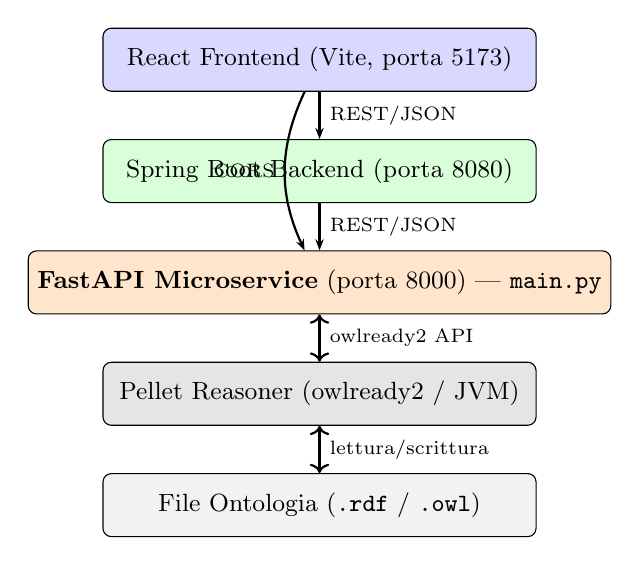
\begin{tikzpicture}[
  node distance=0.6cm,
  box/.style={rectangle, rounded corners=3pt, draw,
              minimum width=5.5cm, minimum height=0.8cm,
              align=center, font=\small},
  arrow/.style={-{Stealth[length=4pt]}, thick},
]
  \node[box, fill=blue!15] (react)   {React Frontend (Vite, porta 5173)};
  \node[box, fill=green!15,  below=of react]   (spring)  {Spring Boot Backend (porta 8080)};
  \node[box, fill=orange!20, below=of spring]  (fastapi) {\textbf{FastAPI Microservice} (porta 8000) --- \texttt{main.py}};
  \node[box, fill=gray!20,   below=of fastapi] (pellet)  {Pellet Reasoner (owlready2 / JVM)};
  \node[box, fill=gray!10,   below=of pellet]  (rdf)     {File Ontologia (\texttt{.rdf} / \texttt{.owl})};

  \draw[arrow] (react)   -- node[right, font=\scriptsize] {REST/JSON}      (spring);
  \draw[arrow] (spring)  -- node[right, font=\scriptsize] {REST/JSON}      (fastapi);
  \draw[arrow, <->] (fastapi) -- node[right, font=\scriptsize] {owlready2 API}  (pellet);
  \draw[arrow, <->] (pellet)  -- node[right, font=\scriptsize] {lettura/scrittura} (rdf);
  \draw[arrow, bend right=25] (react) to node[left, font=\scriptsize] {CORS} (fastapi);
\end{tikzpicture}
\caption{Posizione del microservizio nell'architettura di sistema.}
\end{figure}

Il frontend React comunica \textit{direttamente} con il microservizio
per alcune operazioni (scatter plot, aggiornamenti in tempo reale),
mentre lo Spring Boot Backend funge da orchestratore per i flussi
applicativi complessi.

% ============================================================
\section{Dipendenze e import}
% ============================================================

\subsection{Librerie standard Python}

\begin{longtable}{L{3.5cm} L{9cm}}
  \toprule
  \textbf{Modulo} & \textbf{Motivazione d'uso} \\
  \midrule
  \endhead
  \texttt{os} & Lettura della variabile d'ambiente \texttt{ONTOLOGY\_PATH};
                enumerazione dei file nella directory di servizio. \\[4pt]
  \texttt{threading} & Avvio del reasoner Pellet in un \textit{daemon thread}
                       separato, in modo da non bloccare il ciclo di eventi
                       ASGI di FastAPI durante il caricamento dell'ontologia. \\[4pt]
  \texttt{tempfile} & Creazione di file temporanei \texttt{.sql} per il
                      pipeline di import RDB2RDF, evitando di mantenere
                      dati in memoria per l'intera durata dell'operazione. \\[4pt]
  {\footnotesize\texttt{contextlib.\allowbreak{}asynccontextmanager}} & Necessario per implementare il
                      \textit{lifespan handler} asincrono richiesto dall'API
                      di FastAPI 0.95+. \\[4pt]
  \texttt{pathlib.Path} & Gestione robusta e cross-platform dei percorsi
                          di file, in alternativa alla concatenazione con
                          \texttt{os.path.join}. \\[4pt]
  \texttt{typing.Optional} & Annotazione di tipi per i parametri di query
                             opzionali negli endpoint. \\
  \bottomrule
\end{longtable}

\noindent \subsection{Dipendenze esterne}

\begin{longtable}{L{3.5cm} L{9cm}}
  \toprule
  \textbf{Libreria} & \textbf{Motivazione d'uso} \\
  \midrule
  \endhead
  \texttt{fastapi} & Framework ASGI ad alte prestazioni per la definizione
                    degli endpoint REST, la validazione automatica degli input
                    (via Pydantic) e la generazione della documentazione
                    OpenAPI. Scelto rispetto a Flask o Django per il
                    supporto nativo all'async, la tipizzazione forte e le
                    prestazioni. \\[4pt]
  \texttt{fastapi.\newline CORSMiddleware} & Middleware per la gestione delle
                    \textit{Cross-Origin Resource Sharing} policy.
                    Necessario perch\'{e} frontend React (porta 5173) e backend
                    Spring Boot (porta 8080) risiedono su origini diverse
                    rispetto al microservizio (porta 8000). \\[4pt]
  \texttt{fastapi.\newline responses.\newline JSONResponse} & Risposta JSON personalizzata
                    usata nell'endpoint \texttt{/import/workers}, dove il
                    body di ritorno non segue un \texttt{response\_model}
                    Pydantic fisso. \\[4pt]
  \texttt{uvicorn} & Server ASGI di produzione (e sviluppo) che esegue
                    l'applicazione FastAPI. Configurato per ascoltare su
                    tutte le interfacce (\texttt{0.0.0.0}) alla porta
                    \texttt{8000}. \\
  \bottomrule
\end{longtable}

\noindent \subsection{Moduli interni}

\texttt{main.py} importa da due moduli interni al progetto:

\paragraph{\texttt{reasoner}} Contiene l'intera logica di accesso
all'ontologia: caricamento, ragionamento con Pellet, esecuzione delle
query SPARQL e mutazione in-memory degli individui. Le funzioni importate
sono elencate nella Tabella~\ref{tab:reasoner-imports}.

\paragraph{\texttt{models}} Definisce tutti i modelli Pydantic
(\texttt{BaseModel}) usati come \texttt{response\_model} degli endpoint.
Garantisce validazione automatica dell'output e la generazione dello
schema OpenAPI. Le classi importate sono elencate nella
Tabella~\ref{tab:models-imports}.

\begin{table}[H]
\centering
\caption{Funzioni importate da \texttt{reasoner}.}
\label{tab:reasoner-imports}
\begin{tabular}{L{5cm} L{8cm}}
\toprule
\textbf{Funzione} & \textbf{Responsabilit\`{a}} \\
\midrule
\texttt{state} & Oggetto singleton che espone lo stato corrente del
                 reasoner (\texttt{loading}, \texttt{ready}, \texttt{error}). \\
\texttt{load\_and\_reason} & Carica l'ontologia e avvia Pellet; eseguita
                             nel thread in background. \\
\texttt{load\_snapshot\_cache} & Pre-carica la cache degli snapshot
                                 per ridurre la latenza delle prime query. \\
\texttt{get\_workers} & SPARQL query Q0: restituisce tutti i \texttt{Person}
                        con almeno un \texttt{isEvaluatedForJob}. \\
\texttt{get\_jobs} & Restituisce tutti i \texttt{Job} con almeno una
                     relazione \texttt{requires}. \\
\texttt{get\_health\_conditions} & Recupera i codici ICF e i qualificatori
                                   di un lavoratore. \\
\texttt{get\_importance\_summary} & Q4: importanza skill/abilit\`{a} per job. \\
\texttt{get\_match\_results} & Q1+Q2: calcola GCS\% e AISA\%. \\
\texttt{get\_skill\_detail} & Q3: dettaglio per coppia (worker, job). \\
\texttt{get\_job\_skill\_profile} & Profilo skill di un job (senza worker). \\
\texttt{set\_selected\_worker} & Muta \texttt{isSelected} in-memory. \\
\texttt{get\_all\_icf\_codes} & Tutti i codici ICF presenti nell'ontologia. \\
\texttt{get\_all\_core\_sets} & Nomi distinti degli ICF core set. \\
\texttt{update\_health\_\allowbreak{}conditions} & Applica batch di modifiche ICF. \\
\texttt{update\_worker\_jobs} & Sostituisce i link \texttt{isEvaluatedForJob}. \\
\texttt{inject\_imported\_workers} & Integra in-memory i nuovi individui
                                     importati via SQL. \\
\bottomrule
\end{tabular}
\end{table}

\begin{table}[H]
\centering
\caption{Classi Pydantic importate da \texttt{models}.}
\label{tab:models-imports}
\begin{tabular}{L{5.5cm} L{7.5cm}}
\toprule
\textbf{Classe} & \textbf{Utilizzo} \\
\midrule
\texttt{StatusResponse} & Risposta \texttt{GET /status}. \\
\texttt{OntologyStats} & Statistiche dell'ontologia incluse nello status. \\
\texttt{WorkerSummary} & Elemento di lista in \texttt{GET /workers}. \\
\texttt{WorkerDetail} & Risposta \texttt{GET /workers/\{id\}}. \\
\texttt{JobSummary} & Elemento di lista in \texttt{GET /jobs}. \\
\texttt{JobSkillProfileEntry} & Risposta \texttt{GET /jobs/\{id\}/profile}. \\
\texttt{HealthConditionsResponse} & Risposta \texttt{GET /health-conditions}. \\
\texttt{ImportanceEntry} & Elemento di lista in \texttt{GET /jobs/\{id\}/importance}. \\
\texttt{MatchResult} & Risposta \texttt{GET /match} e varianti. \\
\texttt{MatchDetailRequest} & Request body \texttt{POST /match/detail}. \\
\texttt{SkillDetailResponse} & Risposta \texttt{POST /match/detail}. \\
\texttt{SelectWorkerRequest} & Request body \texttt{POST /workers/select}. \\
\texttt{SelectWorkerResponse} & Risposta \texttt{POST /workers/select}. \\
\texttt{IcfCodeEntry} & Elemento di lista in \texttt{GET /icf-codes}. \\
\texttt{HcChangeItem} & Singola modifica ICF nel batch update. \\
\texttt{UpdateHCRequest} & Request body \texttt{POST /health-conditions/.../update}. \\
\texttt{UpdateHCResponse} & Risposta \texttt{POST /health-conditions/.../update}. \\
\texttt{UpdateWorkerJobsRequest} & Request body \texttt{POST /workers/.../jobs/update}. \\
\texttt{UpdateWorkerJobsResponse} & Risposta \texttt{POST /workers/.../jobs/update}. \\
\bottomrule
\end{tabular}
\end{table}

% ============================================================
\section{Ciclo di vita dell'applicazione (Lifespan)}
% ============================================================

\subsection{Motivazione del pattern lifespan}

FastAPI, a partire dalla versione 0.95, ha deprecato gli event handler
\texttt{on\_event("startup")} in favore del pattern basato su
\texttt{@asynccontextmanager} e il parametro \texttt{lifespan=} del
costruttore \texttt{FastAPI()}. Questo approccio \`{e} preferibile per due
ragioni:
\begin{enumerate}
  \item \`{E} compatibile con la gestione di risorse asincrone (connection pool,
        client HTTP, ecc.) tramite la sintassi \texttt{async with}.
  \item Garantisce che il cleanup venga sempre eseguito, anche in caso di
        eccezioni durante lo startup.
\end{enumerate}

\begin{infobox}[Scelta progettuale --- Thread vs. Task asincrono]
Il reasoner Pellet viene avviato in un \textbf{\texttt{threading.Thread}},
non in una \texttt{asyncio.Task}. La motivazione \`{e} che owlready2 e la JVM
sottostante eseguono operazioni bloccanti di I/O e CPU che non sono
compatibili con il loop asincrono di asyncio. Usare un thread nativo
permette al loop ASGI di restare reattivo durante il caricamento
dell'ontologia (che pu\`{o} durare 30--120 secondi), consentendo al server di
rispondere gi\`{a} al polling di \texttt{GET /status}.
\end{infobox}

\subsection{Sequenza di inizializzazione}

\begin{lstlisting}[caption={Lifespan handler --- startup sequence (\texttt{main.py}, righe 76--104).}]
@asynccontextmanager
async def lifespan(app: FastAPI):
    rdf_path = os.environ.get("ONTOLOGY_PATH", "")

    # 1) Verifica/genera il file di mapping R2RML
    try:
        from import_workers.importer import ensure_mapping
        ...
        ensure_mapping(ontology_file, mapping_file)
    except Exception as _map_err:
        logging.warning("[startup] Could not ensure mapping: %s", _map_err)

    # 2) Pre-carica la snapshot cache (prima che Pellet finisca)
    load_snapshot_cache(rdf_path)

    # 3) Avvia Pellet in un daemon thread
    thread = threading.Thread(
        target=load_and_reason,
        args=(rdf_path,),
        daemon=True,
        name="pellet-reasoner",
    )
    thread.start()
    yield   # <-- l'applicazione gira qui
    # cleanup: nulla da fare; owlready2 gestisce la JVM
\end{lstlisting}

\noindent I tre passi dello startup hanno il seguente significato:

\begin{enumerate}
  \item \textbf{Generazione del mapping R2RML} --- Prima che qualsiasi import
        SQL possa avvenire, deve esistere un file di mapping
        (\texttt{rientra\_mapping.ttl}) che descrive come trasformare le
        tabelle relazionali in triple RDF. La funzione \texttt{ensure\_mapping}
        lo genera a partire dall'ontologia se non \`{e} gi\`{a} presente. Eventuali
        errori in questa fase non bloccano l'avvio (solo un \texttt{warning}),
        perch\'{e} la funzionalit\`{a} di import \`{e} opzionale rispetto al ragionamento.

  \item \textbf{Snapshot cache} --- La funzione \texttt{load\_snapshot\_cache}
        carica una versione pre-computata dei risultati SPARQL
        (se disponibile), in modo che le prime richieste degli endpoint
        non debbano aspettare il completamento di Pellet.

  \item \textbf{Avvio di Pellet} --- Il thread \texttt{pellet-reasoner} \`{e}
        marcato come \textit{daemon}: viene terminato automaticamente quando
        il processo principale termina, evitando zombie JVM.
\end{enumerate}

\begin{figure}[htbp]
\centering
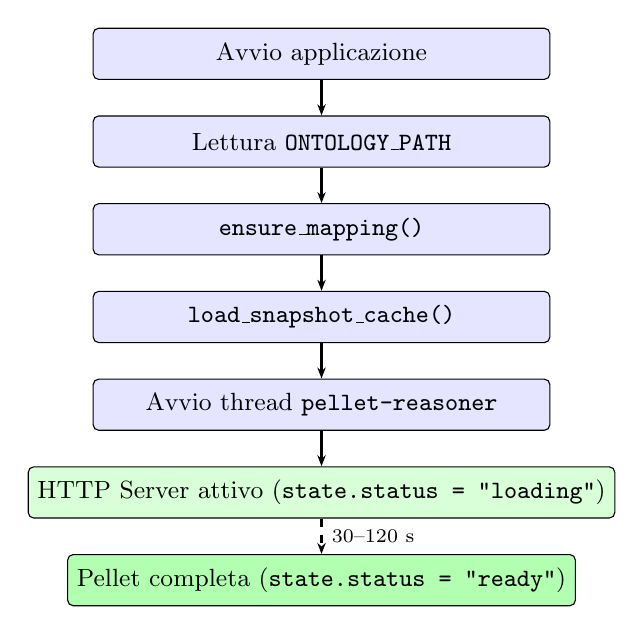
\begin{tikzpicture}[
  node distance=0.45cm,
  block/.style={rectangle, rounded corners=2pt, draw, fill=blue!10,
                minimum width=5.8cm, minimum height=0.65cm, align=center,
                font=\small},
  arrow/.style={-{Stealth[length=4pt]}, thick},
]
  \node[block] (start)  {Avvio applicazione};
  \node[block, below=of start]  (env)    {Lettura \texttt{ONTOLOGY\_PATH}};
  \node[block, below=of env]    (map)    {\texttt{ensure\_mapping()}};
  \node[block, below=of map]    (snap)   {\texttt{load\_snapshot\_cache()}};
  \node[block, below=of snap]   (thread) {Avvio thread \texttt{pellet-reasoner}};
  \node[block, below=of thread, fill=green!15] (ready)
    {HTTP Server attivo (\texttt{state.status = "loading"})};
  \node[block, below=of ready,  fill=green!30] (done)
    {Pellet completa (\texttt{state.status = "ready"})};

  \draw[arrow] (start)  -- (env);
  \draw[arrow] (env)    -- (map);
  \draw[arrow] (map)    -- (snap);
  \draw[arrow] (snap)   -- (thread);
  \draw[arrow] (thread) -- (ready);
  \draw[arrow, dashed]  (ready) -- (done)
    node[midway, right, font=\scriptsize] {30--120 s};
\end{tikzpicture}
\caption{Sequenza temporale di avvio del microservizio.}
\end{figure}

% ============================================================
\section{Configurazione dell'applicazione FastAPI}
% ============================================================

\subsection{Istanza dell'applicazione}

\begin{lstlisting}[caption={Creazione dell'istanza FastAPI.}]
app = FastAPI(
    title="Rientr@ Semantic Microservice",
    description=("REST API exposing the Rientr@ ontology reasoning results. "
                 "Loads an RDF ontology, runs Pellet (DL reasoner) with SWRL rules, "
                 "and serves SPARQL query outputs as structured JSON."),
    version="1.0.0",
    lifespan=lifespan,
)
\end{lstlisting}

\noindent I metadati \texttt{title}, \texttt{description} e \texttt{version}
popolano automaticamente la documentazione OpenAPI disponibile a
\texttt{http://localhost:8000/docs} (Swagger UI) e
\texttt{http://localhost:8000/redoc} (ReDoc). Dichiararli esplicitamente
invece di usare i default (\textit{``FastAPI''}, \textit{``''}, \textit{``0.1.0''})
serve a tre scopi concreti: (1) i client generati automaticamente dalla
specifica OpenAPI includono il titolo nel nome del package; (2) Spring Boot
e il frontend possono rilevare la versione tramite \texttt{/openapi.json}
senza parsing di header HTTP; (3) la descrizione appare nel campo
\texttt{info.description} della specifica, che strumenti come Postman e
Insomnia mostrano agli sviluppatori che integrano il servizio.

\subsection{Middleware CORS}

\begin{lstlisting}[caption={Configurazione del CORS middleware.}]
app.add_middleware(
    CORSMiddleware,
    allow_origins=[
        "http://localhost:5173",   # Vite / React dev server
        "http://localhost:3000",   # alternative React port
        "http://localhost:8080",   # Spring Boot backend
        "http://127.0.0.1:5173",
        "http://127.0.0.1:8080",
    ],
    allow_credentials=True,
    allow_methods=["*"],
    allow_headers=["*"],
)
\end{lstlisting}

\noindent \begin{warningbox}[Nota di sicurezza --- CORS in produzione]
La configurazione attuale consente credenziali (\texttt{allow\_credentials=True})
e tutti i metodi/header per le origini elencate. Per un deploy in produzione
\`{e} necessario:
\begin{enumerate}
  \item Sostituire le origini hardcoded con variabili d'ambiente.
  \item Limitare \texttt{allow\_methods} e \texttt{allow\_headers} ai soli
        valori necessari.
  \item Valutare l'uso di HTTPS.
\end{enumerate}
\end{warningbox}

La scelta di listare esplicitamente le origini anzich\'{e} usare
\texttt{allow\_origins=["*"]} \`{e} intenzionale: con
\texttt{allow\_credentials=True} i browser rifiutano il wildcard, quindi
le origini devono essere elencate esplicitamente.

% ============================================================
\section{Guard di disponibilit\`{a} del reasoner}
% ============================================================

\subsection{La funzione \texttt{\_require\_ready()}}

\begin{lstlisting}[caption={Guard per lo stato del reasoner.}]
def _require_ready() -> None:
    if state.status == "loading":
        raise HTTPException(
            status_code=503,
            detail={
                "status" : "loading",
                "message": "Ontology is still being loaded...",
            },
        )
    if state.status == "error":
        raise HTTPException(
            status_code=500,
            detail={"status": "error", "message": state.message},
        )
\end{lstlisting}

\noindent Ogni endpoint (tranne \texttt{GET /status}) chiama \texttt{\_require\_ready()}
come prima operazione. Questa scelta garantisce:

\begin{itemize}
  \item \textbf{Fail-fast}: il client riceve immediatamente un errore
        significativo invece di attendere una timeout o ricevere dati parziali.
  \item \textbf{Coerenza semantica}: un \texttt{503 Service Unavailable}
        segnala al client che la risorsa \textit{esiste} ma non \`{e} ancora
        disponibile (a differenza di un \texttt{404}), permettendo una
        strategia di retry con backoff esponenziale.
  \item \textbf{Separazione stato/logica}: tutta la gestione dello stato
        \`{e} centralizzata in una sola funzione, rendendo gli endpoint
        focalizzati sulla logica di business.
\end{itemize}

Il mapping eccezione $\rightarrow$ codice HTTP segue criteri semantici precisi:
\texttt{KeyError} produce 404 (la risorsa non esiste nell'ontologia, non
\`{e} un errore del client), \texttt{RuntimeError} produce 503 (la risorsa
esiste ma non \`{e} temporaneamente disponibile, ad esempio per un re-reasoning
in corso). Un 422 Unprocessable Entity sarebbe semanticamente scorretto per
questi casi: 422 indica che la sintassi della richiesta \`{e} valida ma il
contenuto non pu\`{o} essere elaborato, mentre qui il problema \`{e} sempre
nella disponibilit\`{a} della risorsa, non nel formato della richiesta.

\begin{table}[H]
\centering
\caption{Codici HTTP restituiti dalla guard in base allo stato.}
\begin{tabular}{C{3cm} C{2.5cm} L{6cm}}
\toprule
\textbf{stato} & \textbf{HTTP} & \textbf{Significato} \\
\midrule
\texttt{loading} & 503 & Pellet non ha ancora completato; riprova pi\`{u} tardi. \\
\texttt{error}   & 500 & Errore irrecuperabile durante il caricamento. \\
\texttt{ready}   & (nessun errore) & Elaborazione continua normalmente. \\
\bottomrule
\end{tabular}
\end{table}

% ============================================================
\section{Endpoint REST}
% ============================================================

\subsection{Panoramica}

Il microservizio espone \textbf{17 endpoint} raggruppati in 5 tag
tematici. La tabella seguente fornisce una visione sinottica.

I cinque tag (\textit{Service}, \textit{Workers}, \textit{Jobs},
\textit{Matching}, \textit{Health Conditions}, \textit{Import}) rispecchiano
la struttura delle risorse ontologiche, non la struttura interna del codice.
Questa scelta garantisce che la documentazione OpenAPI sia leggibile da un
clinico o un ontology engineer, non solo da un programmatore. Il tag
\textit{Import} \`{e} separato dagli altri perch\'{e} l'operazione di import
\`{e} distruttiva (modifica il file RDF) e lenta (avvia la pipeline RDB2RDF):
isolarla in un tag distinto segnala visivamente la sua natura eccezionale
rispetto alle operazioni di lettura.

\begin{longtable}{L{1.0cm} L{4.5cm} L{1.6cm} L{5.4cm}}
  \toprule
  \textbf{Tag} & \textbf{Path} & \textbf{Metodo} & \textbf{Descrizione} \\
  \midrule
  \endhead
  {\small Svc} & \texttt{/status} & GET & Stato e metriche del servizio. \\[3pt]
  \multirow{4}{*}{\small Wk.}
    & \texttt{/workers} & GET & Lista tutti i lavoratori. \\
    & \texttt{/workers/\allowbreak\{id\}} & GET & Dettaglio singolo lavoratore. \\
    & \texttt{/workers/select} & POST & Seleziona il lavoratore attivo. \\
    & \texttt{/workers/\allowbreak\{id\}/\allowbreak jobs/update} & POST & Aggiorna i job assegnati. \\[3pt]
  \multirow{3}{*}{\small Jobs}
    & \texttt{/jobs} & GET & Lista tutti i job. \\
    & \texttt{/jobs/\allowbreak\{id\}/\allowbreak importance} & GET & Importanza skill (Q4). \\
    & \texttt{/jobs/\allowbreak\{id\}/profile} & GET & Profilo skill del job. \\[3pt]
  \multirow{3}{*}{\small M.}
    & \texttt{/match} & GET & GCS\%/AISA\% per tutti i selezionati. \\
    & \texttt{/match?\allowbreak worker\_id=} & GET & Filtro su worker specifico. \\
    & \texttt{/match/\allowbreak\{id\}} & GET & Matching per worker (path param). \\
    & \texttt{/match/detail} & POST & Dettaglio skill per coppia (Q3). \\[3pt]
  {\small HC}
    & \texttt{/health-cond./\allowbreak\{id\}} & GET & Codici ICF del lavoratore. \\
    & \texttt{/health-conditions/\allowbreak\{id\}/update} & POST & Aggiorna le condizioni ICF. \\
    & \texttt{/icf-codes} & GET & Tutti i codici ICF disponibili. \\
    & \texttt{/core-sets} & GET & Nomi dei core set ICF. \\[3pt]
  {\small Imp.}
    & \texttt{/import/workers} & POST & Import da file SQL (RDB2RDF). \\
  \bottomrule
\end{longtable}

\noindent \subsection{Tag: Service}

\subsubsection{\texttt{GET /status}}

\textbf{Scopo:} Unico endpoint che non richiede lo stato \texttt{ready}.
Restituisce le metriche correnti del reasoner ed \`{e} progettato per il
polling periodico da parte del frontend durante il warm-up.

\textbf{Response model:} \texttt{StatusResponse}

\textbf{Campi notevoli della risposta:}
\begin{itemize}[noitemsep]
  \item \texttt{status}: \texttt{"loading"} | \texttt{"ready"} | \texttt{"error"}
  \item \texttt{elapsed\_pellet}: tempo in secondi impiegato da Pellet.
  \item \texttt{stats}: oggetto \texttt{OntologyStats} (numero classi,
        individui, propriet\`{a}, ecc.).
\end{itemize}

\subsection{Tag: Workers}

\subsubsection{\texttt{GET /workers}}

Restituisce tutti gli individui di classe \texttt{Person} che hanno
almeno una tripla \texttt{isEvaluatedForJob}. Questo filtro esclude le
persone che esistono nell'ontologia ma non sono state ancora associate
a nessun profilo lavorativo, garantendo che la lista sia sempre
actionable dal punto di vista applicativo.

\subsubsection{\texttt{GET /workers/\{worker\_id\}}}

Navigazione per ID. Se il lavoratore non esiste nell'ontologia viene
restituito un \texttt{404 Not Found} con un messaggio esplicito.
Il pattern usato (\texttt{next(..., None)} seguito da controllo esplicito)
\`{e} preferito a una ricerca con eccezione perch\'{e} rende il codice pi\`{u}
leggibile e l'intento pi\`{u} chiaro.

\subsubsection{\texttt{POST /workers/select}}

\begin{lstlisting}[caption={Selezione del lavoratore attivo.}]
# Request body
{ "worker_id": "Patient1" }
\end{lstlisting}

\noindent Muta in-memory il flag \texttt{isSelected} dell'ontologia owlready2:
deseleziona il lavoratore precedentemente attivo e seleziona il nuovo.
Deve essere chiamato \textit{prima} di \texttt{GET /match/\{worker\_id\}},
perch\'{e} la query SPARQL di matching filtra su \texttt{FILTER(?selected = true)}.

\begin{infobox}[Scelta progettuale --- mutazione in-memory]
La modifica di \texttt{isSelected} non viene persistita su file RDF.
Questo \`{e} intenzionale: la selezione \`{e} uno stato di sessione effimero,
non una propriet\`{a} dati permanente. Persistere ogni selezione comporterebbe
riscrittura frequente del file RDF e potenziali race condition nel caso
di accessi concorrenti.
\end{infobox}

\subsubsection{\texttt{POST /workers/\{worker\_id\}/jobs/update}}

Sostituisce atomicamente tutti i link \texttt{isEvaluatedForJob} del
lavoratore. Dopo la mutazione, l'ontologia viene salvata su disco,
Pellet viene rieseguito e la snapshot cache viene aggiornata, in modo
che le chiamate successive a \texttt{/match} riflettano immediatamente
i nuovi assegnamenti. Questo garantisce la coerenza dei dati tra
operazioni successive senza richiedere un riavvio del servizio.

\subsection{Tag: Jobs}

Gli endpoint del tag Jobs usano esclusivamente il metodo \textbf{GET}
perch\'{e} sono operazioni di \textit{sola lettura} sul grafo ontologico:
non modificano l'ontologia, sono idempotenti e cacheabili. Questa
conformit\`{a} alla semantica HTTP permette a proxy, CDN e browser di
mettere in cache le risposte (anche se nel contesto desktop corrente
non ci sono proxy intermedi, la conformit\`{a} facilita future
integrazioni web).

\subsubsection{\texttt{GET /jobs/\{job\_id\}/importance}}

Implementa la \textbf{query semantica Q4}: restituisce la ripartizione
dell'importanza delle skill/abilit\`{a} per un dato job, organizzata per
livello di importanza (\texttt{isVeryImportantFor},
\texttt{isImportantFor}, ecc.), inferita da Pellet attraverso le
regole SWRL 9--12.

\subsubsection{\texttt{GET /jobs/\{job\_id\}/profile}}

Restituisce il profilo completo delle skill richieste da un job con i
relativi punteggi O*NET grezzi (0--100). Non coinvolge alcun lavoratore:
\`{e} pensato per costruire grafici radar o di "inclinazione" indipendentemente
da qualsiasi condizione di salute.

\subsection{Tag: Matching}

Il matching \`{e} il cuore funzionale del sistema. Il microservizio espone
tre livelli di dettaglio invece di un solo endpoint generico, per due ragioni.
Prima ragione: \textbf{granularit\`{a} delle query SPARQL}. Le tre query (Q0,
Q1+Q2, Q3) hanno costo computazionale molto diverso: Q3 (\texttt{hasSpecificCriticality}
per ogni skill di una coppia) \`{e} dieci volte pi\`{u} lenta di Q1+Q2
(aggregato per worker). Esporre granularit\`{a} separate permette al frontend
di caricare prima la visione d'insieme (scatter plot) e poi il dettaglio on-demand.
Seconda ragione: \textbf{separazione degli use case}. \texttt{GET /match}
alimenta la KPI strip e lo scatter plot; \texttt{GET /match/\{id\}} permette
il deep link a un worker specifico da Spring Boot; \texttt{POST /match/detail}
\`{e} chiamato solo quando l'utente apre la tabella skill.

\begin{enumerate}
  \item \texttt{GET /match} --- risultati aggregati per tutti i lavoratori
        selezionati (o filtrati per \texttt{worker\_id}).
  \item \texttt{GET /match/\{worker\_id\}} --- risultati per un singolo
        lavoratore (path parameter, restituisce 404 se assente).
  \item \texttt{POST /match/detail} --- breakdown per-skill per una specifica
        coppia (worker, job). Usa POST anzich\'{e} GET perch\'{e} il body
        della richiesta contiene due ID che semanticamente formano un
        ``oggetto di ricerca'', non filtri di una collezione.
\end{enumerate}

\subsubsection{Query Q1+Q2 --- GCS\% e AISA\%}

I due indicatori principali del sistema Rientr@ sono:

\begin{itemize}
  \item \textbf{GCS\% (General Criticality Score)}: misura la criticit\`{a}
        complessiva del profilo di salute del lavoratore rispetto al job.
  \item \textbf{AISA\% (Amount of Impaired Skill/Abilities)}: percentuale
        di skill/abilit\`{a} richieste dal job che risultano compromesse dalla
        condizione di salute del lavoratore.
\end{itemize}

Il campo \texttt{suitability} viene derivato dalle soglie definite in
Fig.~4 del paper Rientr@:

\begin{align}
  \text{SUITABLE} &: \text{GCS} < -0.5 \cdot \text{AISA} + 15.5 \\
  \text{NOT SUITABLE} &: \text{GCS} > -0.5 \cdot \text{AISA} + 21 \\
  \text{SUITABLE WITH PRECAUTIONS} &: \text{altrimenti}
\end{align}

\subsubsection{Query Q3 --- Dettaglio per coppia (worker, job)}
\vspace{2pt}
\begin{lstlisting}[caption={Request body per \texttt{POST /match/detail}.}]
{ "worker_id": "Patient1", "job_id": "Job_AssemblyWorker" }
\end{lstlisting}

\noindent Restituisce per ogni skill/abilit\`{a}:
\begin{itemize}[noitemsep]
  \item Punteggio O*NET di importanza (0--100).
  \item Anchor di importanza [0--3].
  \item Qualificatore ICF del lavoratore.
  \item Criticality Score: $CS = \text{qualifier} \times \text{anchor}$.
  \item CS normalizzato: $\widehat{CS} = CS / 12$.
  \item Label di criticit\`{a} (da \textit{not critical} a
        \textit{extremely critical}).
\end{itemize}

\subsection{Tag: Health Conditions}

\subsubsection{\texttt{GET /health-conditions/\{worker\_\allowbreak{}id\}}}

Alimenta la tabella "Current Health Conditions" nel frontend React.
Restituisce i codici ICF con i rispettivi qualificatori (0--4) associati
al profilo di salute del lavoratore.

\subsubsection{\texttt{POST /health-conditions/\{worker\_\allowbreak{}id\}/update}}

Applica un batch di modifiche (\texttt{add}, \texttt{remove},
\texttt{modify}) al profilo ICF del lavoratore \textit{in-memory}.
Nessun file RDF viene riscritto in questa operazione, che \`{e} quindi
reversibile tra sessioni.

\begin{lstlisting}[caption={Request body per l'update delle condizioni ICF.}]
{
  "worker_id": "Patient1",
  "changes": [
    { "icf_code": "b1408", "action": "add",    "qualifier": 2 },
    { "icf_code": "d410",  "action": "modify", "qualifier": 3 },
    { "icf_code": "b280",  "action": "remove", "qualifier": null }
  ]
}
\end{lstlisting}

\noindent \subsubsection{\texttt{GET /icf-codes} e \texttt{GET /core-sets}}

\texttt{/icf-codes} \`{e} un endpoint separato da
\texttt{/health-cond./\allowbreak\{id\}} per una ragione di frequenza di accesso:
le condizioni di salute di un worker vengono ricaricate ad ogni selezione
del worker (potenzialmente decine di volte per sessione); il catalogo ICF
completo viene caricato solo quando l'utente apre la wizard di modifica
(una volta per sessione al massimo). Accoppiarli in un singolo endpoint
significherebbe trasferire centinaia di entry ICF ad ogni cambio worker,
aumentando la latenza percepita. La separazione rispetta il principio di
\textit{caricamento lazy}: il catalogo pesante viene caricato solo quando
serve.

Questi due endpoint forniscono i dati necessari al frontend per
popolare le interfacce di selezione nella procedura guidata "Modify
Health Condition":
\begin{itemize}[noitemsep]
  \item \texttt{/icf-codes}: restituisce tutti i codici ICF presenti
        nell'ontologia via triple \texttt{involvesICFCode}.
  \item \texttt{/core-sets}: lista ordinata dei core set ICF distinti
        (es. \textit{Stroke}, \textit{Hearing Loss}, \textit{Low Back Pain}).
\end{itemize}

\subsection{Tag: Import}

\subsubsection{\texttt{POST /import/workers}}

\begin{infobox}[Pipeline RDB2RDF via R2RML]
Questo \`{e} l'endpoint pi\`{u} complesso del microservizio. Implementa una
pipeline completa di importazione dati strutturati in formato SQL
nell'ontologia RDF.
\end{infobox}

\textbf{Flusso operativo:}

\begin{enumerate}
  \item Il client invia il file \texttt{.sql} come body raw
        (\texttt{Content-Type: application/octet-stream}).
        Il nome del file pu\`{o} essere trasmesso nell'header
        \texttt{X-Filename}.
  \item Il body viene letto con \texttt{await request.body()},
        senza richiedere \texttt{python-multipart} (scelta che riduce
        le dipendenze).
  \item Il file viene scritto in un file temporaneo con
        \texttt{tempfile.NamedTemporaryFile}.
  \item Viene verificata la presenza del file di mapping R2RML
        (\texttt{rientra\_mapping.ttl}); se assente, viene generato
        da \texttt{ensure\_mapping()}.
  \item La funzione \texttt{import\_sql\_dataset()} esegue la
        trasformazione RDB2RDF e aggiorna il file ontologico.
  \item Il file temporaneo viene eliminato nel blocco \texttt{finally},
        garantendo la pulizia anche in caso di errore.
  \item Se l'import ha aggiunto nuovi individui, viene chiamata
        \texttt{inject\_imported\_workers()} per aggiornare
        l'ontologia in-memory senza riavviare Pellet.
\end{enumerate}

\begin{lstlisting}[caption={Struttura della risposta di \texttt{POST /import/workers}.}]
{
  "persons_added"  : 3,
  "persons_skipped": 0,
  "icf_valid"      : 42,
  "icf_skipped"    : 2,
  "jobs_valid"     : 7,
  "jobs_skipped"   : 1,
  "new_person_ids" : ["LucaMartini", "ElenaConti", "GiuseppeFerrari"],
  "skipped_ids"    : [],
  "backup_path"    : "/abs/path/Rientra.rdf.bak",
  "error"          : null
}
\end{lstlisting}

\noindent Il campo \texttt{backup\_path} indica dove \`{e} stato salvato il backup
dell'ontologia prima della modifica, permettendo un eventuale rollback
manuale.

% ============================================================
\section{Gestione degli errori}
% ============================================================

\subsection{Strategia generale}

Tutti gli endpoint seguono il pattern:

\begin{lstlisting}[caption={Pattern di gestione degli errori degli endpoint.}]
def endpoint(...):
    _require_ready()
    try:
        data = get_something(...)
        return ResponseModel(**data)
    except HTTPException:
        raise                  # propaga errori gia' tipizzati
    except KeyError as exc:
        raise HTTPException(status_code=404, detail=str(exc)) from exc
    except RuntimeError as exc:
        raise HTTPException(status_code=503, detail=str(exc)) from exc
    except Exception as exc:
        raise HTTPException(status_code=500, detail=str(exc)) from exc
\end{lstlisting}

\noindent \subsection{Gerarchia dei codici di errore}

\begin{table}[H]
\centering
\caption{Mapping eccezioni $\rightarrow$ codici HTTP.}
\begin{tabular}{L{3.5cm} C{2cm} L{6.5cm}}
\toprule
\textbf{Eccezione Python} & \textbf{HTTP} & \textbf{Significato applicativo} \\
\midrule
\texttt{state == "loading"} & 503 & Reasoner ancora in esecuzione. \\
\texttt{state == "error"}   & 500 & Errore irrecuperabile del reasoner. \\
\texttt{KeyError}           & 404 & Risorsa (worker/job) non trovata. \\
\texttt{RuntimeError}       & 503 & Risorsa temporaneamente non disponibile. \\
\texttt{Exception} (generico) & 500 & Errore interno non previsto. \\
\bottomrule
\end{tabular}
\end{table}

% ============================================================
\section{Entrypoint di sviluppo}
% ============================================================

\begin{lstlisting}[caption={Avvio diretto con Uvicorn per lo sviluppo.}]
if __name__ == "__main__":
    import uvicorn
    uvicorn.run(
        "main:app",
        host="0.0.0.0",
        port=8000,
        reload=False,   # True solo in sviluppo
        log_level="info",
    )
\end{lstlisting}

\noindent Il flag \texttt{reload=False} \`{e} impostato di default anche nell'entrypoint
di sviluppo, perch\'{e} il reload automatico di Uvicorn riavvierebbe
il thread Pellet ad ogni modifica del codice, con tempi inaccettabili
(30--120 s). In fase di sviluppo attivo, si raccomanda di:
\begin{enumerate}
  \item Modificare solo i file che non toccano il reasoner
        (\texttt{main.py}, \texttt{models.py}).
  \item Usare \texttt{--reload} solo quando si lavora su parti
        che non richiedono il warm-up di Pellet.
\end{enumerate}

Il comando raccomandato per il deploy \`{e} invece:
\begin{lstlisting}[language=bash, caption={Comando di avvio in produzione.}]
uvicorn main:app --host 0.0.0.0 --port 8000 --reload
\end{lstlisting}

% ============================================================
\section{Modulo \texttt{models.py} --- Schemi Pydantic v2}
% ============================================================

\subsection{Ruolo e motivazione del modulo}

\texttt{models.py} centralizza la definizione di \textbf{tutti i modelli
di dati} del microservizio, sia per le risposte (\textit{response models})
che per i corpi delle richieste (\textit{request bodies}). La scelta di
isolare questi schemi in un modulo dedicato, anzich\'{e} dichiararli inline
negli endpoint, risponde a tre obiettivi:

\begin{enumerate}
  \item \textbf{Riusabilit\`{a}}: lo stesso modello pu\`{o} essere importato
        da \texttt{main.py} e, in futuro, da test automatici o da client
        generati.
  \item \textbf{Documentazione automatica}: FastAPI legge le annotazioni
        Pydantic e genera automaticamente lo schema JSON (OpenAPI 3.1)
        esposto a \texttt{/docs} e \texttt{/openapi.json}, comprese le
        descrizioni dei campi via \texttt{Field(description=...)}.
  \item \textbf{Validazione in ingresso}: i \textit{request bodies}
        definiti come \texttt{BaseModel} vengono validati da Pydantic
        prima che la funzione endpoint venga eseguita; un payload non
        valido produce automaticamente un \texttt{422 Unprocessable Entity}
        con un messaggio di errore strutturato.
\end{enumerate}

\begin{infobox}[Pydantic v2 vs. v1]
Il modulo usa esplicitamente \textbf{Pydantic v2} (importazione da
\texttt{pydantic} con \texttt{BaseModel} e \texttt{Field}). Le differenze
principali rispetto alla v1 che impattano questo codice sono:
\begin{itemize}[noitemsep]
  \item \texttt{model\_dump()} sostituisce \texttt{dict()} --- usato in
        \texttt{main.py} per serializzare i \texttt{HcChangeItem} prima
        di passarli al reasoner.
  \item La validazione di default \`{e} pi\`{u} rigida sui tipi (es.\
        \texttt{int} non accetta stringhe numeriche senza coercizione).
  \item \texttt{default\_factory=list} sostituisce il vecchio pattern
        \texttt{default=[]}, che in v1 causava il classico bug di
        mutabilit\`{a} degli argomenti di default.
\end{itemize}
\end{infobox}

\subsection{Dipendenze del modulo}

\begin{table}[H]
\centering
\caption{Import di \texttt{models.py}.}
\begin{tabular}{L{4cm} L{8.5cm}}
\toprule
\textbf{Import} & \textbf{Motivazione} \\
\midrule
\texttt{from \_\allowbreak{}\_\allowbreak{}future\_\allowbreak{}\_\allowbreak{} import annotations} &
  Abilita la valutazione lazy delle annotazioni di tipo (PEP 563),
  necessaria per riferimenti forward e compatibilit\`{a} con Python 3.10+
  prima che diventasse default. \\[4pt]
\texttt{typing.Optional} &
  Usato per i campi che possono essere \texttt{None} (es.\
  \texttt{elapsed\_pellet}, \texttt{qualifier}). In Python 3.10+ si
  potrebbe usare \texttt{X | None}, ma \texttt{Optional} mantiene la
  compatibilit\`{a} con toolchain pi\`{u} datate. \\[4pt]
\texttt{pydantic.BaseModel} &
  Classe base di tutti i modelli; fornisce parsing, validazione e
  serializzazione automatica. \\[4pt]
\texttt{pydantic.Field} &
  Permette di arricchire i campi con metadati (descrizione,
  esempi, vincoli numerici) che vengono inclusi nello schema OpenAPI. \\
\bottomrule
\end{tabular}
\end{table}

\subsection{Panoramica dei gruppi di modelli}

I modelli sono organizzati in sette gruppi logici, corrispondenti
ai tag degli endpoint di \texttt{main.py}:

\begin{figure}[htbp]
\centering
\resizebox{\linewidth}{!}{%
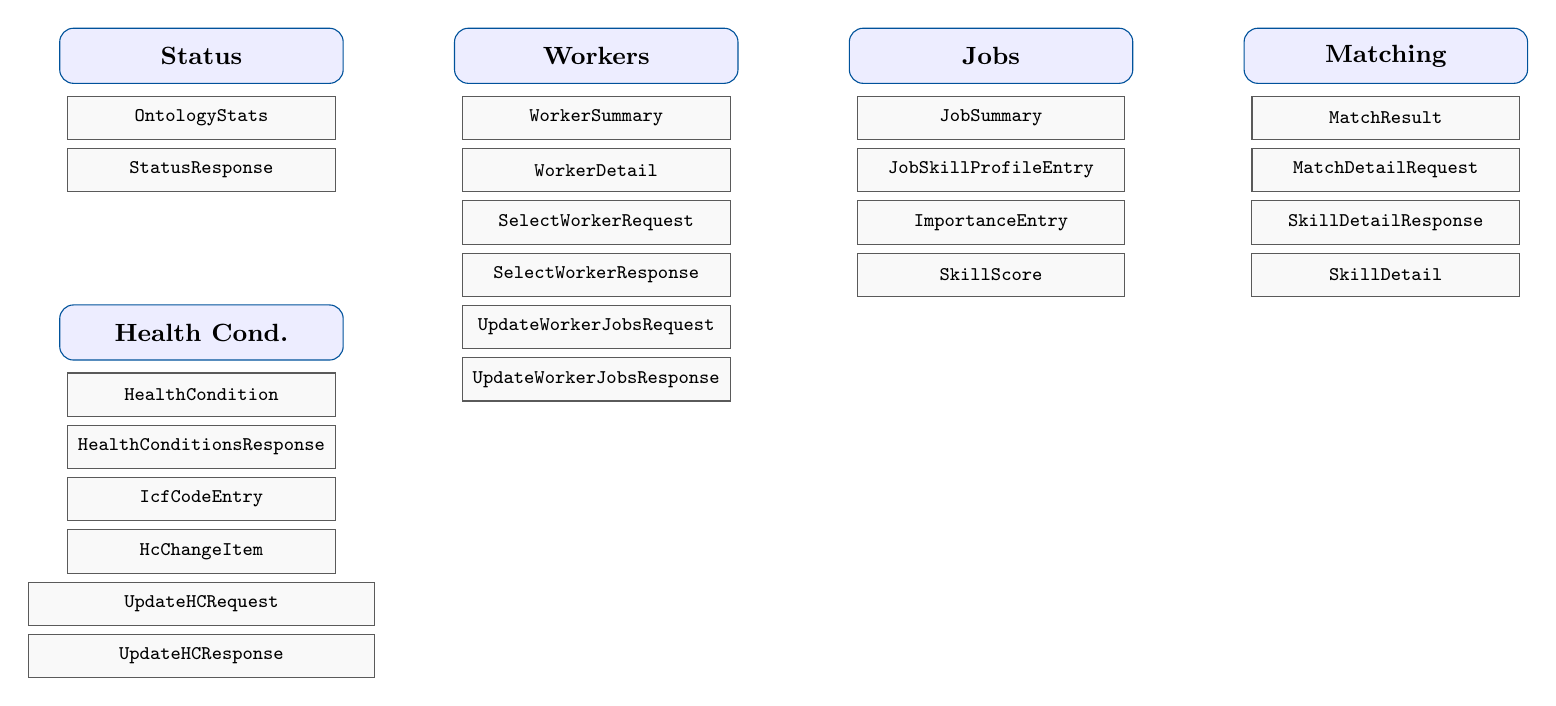
\begin{tikzpicture}[scale=0.85,
  node distance=0.6cm and 1.2cm,
  grp/.style={rectangle, rounded corners=5pt, draw=rientraBlue,
              fill=blue!7, minimum width=3.6cm, minimum height=0.7cm,
              align=center, font=\small\bfseries},
  mod/.style={rectangle, draw=rientraGray, fill=gray!5,
              minimum width=3.4cm, minimum height=0.55cm,
              align=center, font=\ttfamily\scriptsize},
  arr/.style={-{Stealth[length=4pt]}, gray},
]
  % Column 1
  \node[grp] (g1) {Status};
  \node[mod, below=0.15cm of g1] (m1a) {OntologyStats};
  \node[mod, below=0.1cm of m1a] (m1b) {StatusResponse};

  % Column 2
  \node[grp, right=1.4cm of g1] (g2) {Workers};
  \node[mod, below=0.15cm of g2] (m2a) {WorkerSummary};
  \node[mod, below=0.1cm of m2a] (m2b) {WorkerDetail};
  \node[mod, below=0.1cm of m2b] (m2c) {SelectWorkerRequest};
  \node[mod, below=0.1cm of m2c] (m2d) {SelectWorkerResponse};
  \node[mod, below=0.1cm of m2d] (m2e) {UpdateWorkerJobsRequest};
  \node[mod, below=0.1cm of m2e] (m2f) {UpdateWorkerJobsResponse};

  % Column 3
  \node[grp, right=1.4cm of g2] (g3) {Jobs};
  \node[mod, below=0.15cm of g3] (m3a) {JobSummary};
  \node[mod, below=0.1cm of m3a] (m3b) {JobSkillProfileEntry};
  \node[mod, below=0.1cm of m3b] (m3c) {ImportanceEntry};
  \node[mod, below=0.1cm of m3c] (m3d) {SkillScore};

  % Column 4
  \node[grp, right=1.4cm of g3] (g4) {Matching};
  \node[mod, below=0.15cm of g4] (m4a) {MatchResult};
  \node[mod, below=0.1cm of m4a] (m4b) {MatchDetailRequest};
  \node[mod, below=0.1cm of m4b] (m4c) {SkillDetailResponse};
  \node[mod, below=0.1cm of m4c] (m4d) {SkillDetail};

  % Column 5 (below col 1-2, health)
  \node[grp, below=2.8cm of g1] (g5) {Health Cond.};
  \node[mod, below=0.15cm of g5] (m5a) {HealthCondition};
  \node[mod, below=0.1cm of m5a] (m5b) {HealthConditionsResponse};
  \node[mod, below=0.1cm of m5b] (m5c) {IcfCodeEntry};
  \node[mod, below=0.1cm of m5c] (m5d) {HcChangeItem};
  \node[mod, below=0.1cm of m5d, minimum width=4.4cm] (m5e) {\scriptsize UpdateHCRequest};
  \node[mod, below=0.1cm of m5e, minimum width=4.4cm] (m5f) {\scriptsize UpdateHCResponse};
\end{tikzpicture}%
}% end resizebox
\caption{Raggruppamento dei modelli Pydantic per dominio funzionale.}
\end{figure}

\subsection{Gruppo: Status}

\subsubsection{\texttt{OntologyStats}}

\begin{lstlisting}[caption={\texttt{OntologyStats} --- statistiche dell'ontologia.}]
class OntologyStats(BaseModel):
    classes:     int
    individuals: int
    properties:  int
\end{lstlisting}

\noindent Modello ausiliario annidato in \texttt{StatusResponse}. Espone i tre
contatori fondamentali dell'ontologia caricata, utili per diagnostica
e monitoraggio. La scelta di usare un oggetto annidato anzich\'{e} tre
campi flat in \texttt{StatusResponse} migliora la leggibilit\`{a} del
JSON e permette di estendere le statistiche senza modificare la struttura
radice.

\subsubsection{\texttt{StatusResponse}}

\begin{lstlisting}[caption={\texttt{StatusResponse} --- risposta di \texttt{GET /status}.}]
class StatusResponse(BaseModel):
    status:         str   = Field(..., examples=["ready","loading","error"])
    message:        str
    ontology_path:  str   = ""
    elapsed_pellet: Optional[float] = Field(
        None, description="Pellet runtime in seconds")
    stats:          Optional[OntologyStats] = None
\end{lstlisting}

\noindent Il campo \texttt{status} \`{e} una stringa libera (non un \texttt{Literal}
o un \texttt{Enum}) per mantenere la flessibilit\`{a} in caso di stati
futuri. Il valore \texttt{elapsed\_pellet} \`{e} \texttt{Optional[float]}
perch\'{e} non \`{e} disponibile finch\'{e} Pellet non ha completato;
\texttt{stats} \`{e} anch'esso opzionale per lo stesso motivo.

\texttt{ontology\_path} ha come default una stringa vuota anzich\'{e}
\texttt{None} per evitare \texttt{null} nel JSON, che richiederebbe
gestione esplicita nel frontend.

\subsection{Gruppo: Workers}

\subsubsection{\texttt{WorkerSummary} e \texttt{WorkerDetail}}

\begin{lstlisting}[caption={\texttt{WorkerSummary} e \texttt{WorkerDetail}.}]
class WorkerSummary(BaseModel):
    id:                 str
    first_name:         str
    surname:            str
    is_selected:        bool
    evaluated_for_jobs: list[str]

class WorkerDetail(BaseModel):
    id:                 str
    first_name:         str
    surname:            str
    is_selected:        bool
    evaluated_for_jobs: list[str]
\end{lstlisting}

\noindent \begin{infobox}[Nota di design --- WorkerSummary vs WorkerDetail]
I due modelli hanno attualmente la stessa struttura. Questa duplicazione
\`{e} \textbf{intenzionale}: separa concettualmente i due contesti d'uso
(lista vs.\ dettaglio singolo) e permette di aggiungere campi specifici
al dettaglio (es.\ storico delle valutazioni, metadati clinici) senza
modificare la struttura della lista, che potrebbe essere cacheable o
paginata in futuro.
\end{infobox}

I campi \texttt{first\_name} e \texttt{surname} sono distinti (non
concatenati) per permettere ordinamenti e filtri lato client senza
parsing. Il campo \texttt{evaluated\_for\_jobs} \`{e} una lista di
stringhe (IRI locali dei job) anzich\'{e} oggetti \texttt{JobSummary}
annidati, per evitare risposte troppo verbose nella lista workers.

\subsubsection{\texttt{SelectWorkerRequest} e \texttt{SelectWorkerResponse}}

\begin{lstlisting}[caption={Selezione del lavoratore attivo.}]
class SelectWorkerRequest(BaseModel):
    worker_id: str = Field(..., examples=["Patient1"])

class SelectWorkerResponse(BaseModel):
    previous: Optional[str] = Field(
        None, description="ID del worker precedentemente selezionato.")
    selected: str = Field(..., description="ID del worker ora selezionato.")
\end{lstlisting}

\noindent La risposta include \texttt{previous} per permettere al frontend di
aggiornare lo stato UI (es.\ deselezionare il marker precedente nello
scatter plot) senza dover mantenere lo stato localmente o fare una
chiamata aggiuntiva a \texttt{GET /workers}.

\subsubsection{\texttt{UpdateWorkerJobsRequest} e \texttt{UpdateWorkerJobsResponse}}

\begin{lstlisting}[caption={Aggiornamento dei job assegnati a un lavoratore.}]
class UpdateWorkerJobsRequest(BaseModel):
    """Replace the complete set of isEvaluatedForJob links."""
    job_ids: list[str] = Field(
        ...,
        description="Lista ordinata di job ID da assegnare.",
        examples=[["Job_AssemblyWorker", "Job_Carpenter"]],
    )

class UpdateWorkerJobsResponse(BaseModel):
    worker_id:  str
    previous:   list[str] = Field(..., description="Job assegnati prima.")
    assigned:   list[str] = Field(..., description="Job assegnati dopo.")
    unresolved: list[str] = Field(
        default_factory=list,
        description="ID richiesti non trovati nell'ontologia (ignorati).",
    )
\end{lstlisting}

\noindent La semantica di \textbf{sostituzione atomica} (non append) semplifica
la logica client: il frontend invia sempre la lista completa desiderata,
senza dover calcolare diff. Il campo \texttt{unresolved} segnala
silenziosamente gli ID non validi senza far fallire l'intera operazione,
implementando una politica di \textit{partial success}.

\texttt{default\_factory=list} (anzich\'{e} \texttt{default=[]}) \`{e}
la pratica corretta in Pydantic v2 per i campi con default mutabile,
evitando la condivisione accidentale dello stesso oggetto lista tra
istanze diverse.

\subsection{Gruppo: Jobs}

\subsubsection{\texttt{JobSummary}}

\begin{lstlisting}[caption={\texttt{JobSummary} --- elemento di lista job.}]
class JobSummary(BaseModel):
    id:    str
    label: str
\end{lstlisting}

\noindent Modello minimo per la lista dei job. Il campo \texttt{label} contiene
la denominazione leggibile del profilo lavorativo (es.\
\textit{``Assembly Worker''}) distinta dall'IRI locale (\texttt{id}).

\subsubsection{\texttt{JobSkillProfileEntry}}

\begin{lstlisting}[caption={\texttt{JobSkillProfileEntry} --- skill con punteggio O*NET.}]
class JobSkillProfileEntry(BaseModel):
    """One skill/ability required by a job, with its raw O*NET score."""
    id:    str
    score: int = Field(..., description="O*NET importance score [0-100]")
\end{lstlisting}

\noindent Usato da \texttt{GET /jobs/\{id\}/profile}. Il punteggio O*NET grezzo
(0--100) viene qui esposto direttamente, a differenza dell'\texttt{anchor}
[0--3] usato nel matching, perch\'{e} questo endpoint \`{e} pensato per
visualizzazioni radar/inclinazione che richiedono la scala completa.

\subsubsection{\texttt{ImportanceEntry} e \texttt{SkillScore}}

\begin{lstlisting}[caption={Importanza skill per job (Q4).}]
class SkillScore(BaseModel):
    id:    str
    score: int

class ImportanceEntry(BaseModel):
    job_id:           str
    importance_level: str = Field(
        ...,
        examples=["isVeryImportantFor", "isImportantFor",
                  "isSomewhatImportantFor", "isLessImportantFor"],
    )
    skills: list[SkillScore]
\end{lstlisting}

\noindent \texttt{ImportanceEntry} aggrega le skill per \textbf{livello di importanza},
rispecchiando la struttura delle regole SWRL 9--12. Il valore di
\texttt{importance\_level} corrisponde direttamente al nome della
propriet\`{a} OWL inferita da Pellet, mantenendo trasparenza tra
ontologia e API.

\subsection{Gruppo: Matching}

\subsubsection{\texttt{MatchResult}}

\begin{lstlisting}[caption={\texttt{MatchResult} --- coppia (worker, job) con punteggi.}]
class MatchResult(BaseModel):
    worker_id:         str
    job_id:            str
    gcs_pct:           float = Field(..., description="General Criticality Score %")
    aisa_pct:          float = Field(..., description="Amount Impaired SkAb %")
    n_total:           int   = Field(..., description="Numero totale di SkAb valutate")
    n_critical:        int   = Field(..., description="SkAb con CS > 0")
    suitability:       str   = Field(...,
        examples=["SUITABLE","SUITABLE WITH PRECAUTIONS","NOT SUITABLE"])
    suitability_color: str   = Field(...,
        examples=["#22c55e","#f59e0b","#ef4444"])
\end{lstlisting}

\noindent Il campo \texttt{suitability\_color} merita attenzione: incorpora la
logica di colore direttamente nella risposta API. Questa scelta
accoppia leggermente il backend alla presentazione, ma semplifica il
frontend che non deve reimplementare le soglie di Fig.~4 del paper
Rientr@. I tre colori corrispondono al sistema di semaforo verde /
giallo / rosso:

\begin{table}[H]
\centering
\caption{Mapping suitability $\rightarrow$ colore hex.}
\begin{tabular}{L{5.5cm} C{3cm} C{3cm}}
\toprule
\textbf{Suitability} & \textbf{Colore} & \textbf{Hex} \\
\midrule
\texttt{SUITABLE} & Verde & \texttt{\#22c55e} \\
\texttt{SUITABLE WITH PRECAUTIONS} & Ambra & \texttt{\#f59e0b} \\
\texttt{NOT SUITABLE} & Rosso & \texttt{\#ef4444} \\
\bottomrule
\end{tabular}
\end{table}

I colori hex usati corrispondono ai valori \textit{Tailwind CSS} standard
(\texttt{green-500}, \texttt{amber-400}, \texttt{red-500}), coerenti
con la palette del frontend React.

\subsubsection{\texttt{MatchDetailRequest}}

\begin{lstlisting}[caption={Request body per \texttt{POST /match/detail}.}]
class MatchDetailRequest(BaseModel):
    worker_id: str = Field(..., examples=["Patient1"])
    job_id:    str = Field(..., examples=["Job_AssemblyWorker"])
\end{lstlisting}

\noindent La coppia (worker, job) viene trasmessa come \textbf{POST body} anzich\'{e}
come query string o path parameter per due ragioni: (1) semantica REST
pi\`{u} corretta per un'operazione di ricerca complessa; (2) facilitazione
di eventuali estensioni future (aggiunta di filtri, opzioni di calcolo).

\subsubsection{\texttt{SkillDetail} e \texttt{SkillDetailResponse}}

\begin{lstlisting}[caption={\texttt{SkillDetail} --- dettaglio per singola skill (Q3).}]
class SkillDetail(BaseModel):
    id:                str
    score:             int   = Field(..., description="O*NET score [0-100]")
    importance_label:  str   = Field(..., examples=["isVeryImportantFor"])
    anchor:            int   = Field(..., description="Importance anchor [0-3]")
    qualifier:         int   = Field(..., description="ICF qualifier value")
    cs:                int   = Field(..., description="CS = qualifier x anchor")
    cs_normalized:     float = Field(..., description="CS / 12 (normalized)")
    criticality_label: str   = Field(..., examples=["MODERATELY CRITICAL"])
    description:       str   = Field("", description="Descrizione ICF della skill")

class SkillDetailResponse(BaseModel):
    worker_id: str
    job_id:    str
    skills:    list[SkillDetail]
\end{lstlisting}

\noindent \texttt{SkillDetail} \`{e} il modello pi\`{u} ricco del sistema: espone
l'intera catena di calcolo del Criticality Score per ogni skill, dalla
fonte grezza (O*NET) alla classificazione finale. Questo permette al
frontend di costruire tabelle di dettaglio trasparenti e verificabili
dall'utente clinico.

Il campo \texttt{description} ha come default una stringa vuota (non
\texttt{None}) per coerenza con la serializzazione: il frontend
riceve sempre un campo stringa, senza dover gestire il caso
\texttt{null}.

\subsection{Gruppo: Health Conditions}

\subsubsection{\texttt{HealthCondition} e \texttt{HealthConditionsResponse}}

\begin{lstlisting}[caption={Condizione di salute ICF di un lavoratore.}]
class HealthCondition(BaseModel):
    icf_code:      str
    icf_name:      str  = ""
    description:   str  = ""
    core_sets:     list[str] = []
    bf_qualifier:  Optional[int] = None
    ap1_qualifier: Optional[int] = None

class HealthConditionsResponse(BaseModel):
    worker_id:  str
    conditions: list[HealthCondition]
\end{lstlisting}

\noindent \texttt{HealthCondition} modella un singolo codice ICF con i suoi
qualificatori. La distinzione tra \texttt{bf\_qualifier} e
\texttt{ap1\_qualifier} riflette la struttura ICF che prevede
qualificatori separati per \textit{Body Functions/Structures} (b/s) e
\textit{Activities \& Participation} (d). Entrambi sono \texttt{Optional[int]}
perch\'{e} un codice potrebbe non avere entrambi i qualificatori
valorizzati nell'ontologia.

Il campo \texttt{core\_sets} \`{e} una lista di stringhe che identifica
a quali core set ICF appartiene il codice (es.\ ``Stroke'',
``Low Back Pain''), utilizzato dal frontend per filtrare la visualizzazione.

\subsubsection{\texttt{IcfCodeEntry}}

\begin{lstlisting}[caption={\texttt{IcfCodeEntry} --- catalogo ICF per la procedura guidata.}]
class IcfCodeEntry(BaseModel):
    icf_code:    str
    icf_name:    str  = ""
    description: str  = ""
    category:    str  = ""
    core_sets:   list[str] = []
    iri:         str  = ""
\end{lstlisting}

\noindent Rispetto a \texttt{HealthCondition}, questo modello aggiunge:
\begin{itemize}[noitemsep]
  \item \texttt{category}: categoria ICF di primo livello (es.\
        \textit{``Body Functions''}, \textit{``Activities''}), utile
        per raggruppare i codici nella tabella di selezione della wizard.
  \item \texttt{iri}: IRI completo dell'individuo nell'ontologia, necessario
        per operazioni di lookup preciso nel reasoner.
\end{itemize}

I qualificatori sono assenti perch\'{e} \texttt{IcfCodeEntry} rappresenta
il \textit{catalogo} dei codici disponibili, non l'istanza specifica
di un lavoratore.

\subsubsection{\texttt{HcChangeItem}, \texttt{UpdateHealthConditionsRequest} e\\[2pt] \texttt{UpdateHealthConditionsResponse}}

\begin{lstlisting}[caption={Modelli per l'aggiornamento batch delle condizioni ICF.}]
class HcChangeItem(BaseModel):
    icf_code:  str
    action:    str = Field(..., examples=["add","remove","modify"])
    qualifier: Optional[int] = Field(None, ge=0, le=4)

class UpdateHealthConditionsRequest(BaseModel):
    worker_id: str
    changes:   list[HcChangeItem]

class UpdateHealthConditionsResponse(BaseModel):
    worker_id: str
    added:     int
    removed:   int
    modified:  int
\end{lstlisting}

\noindent Il vincolo \texttt{ge=0, le=4} su \texttt{qualifier} rispecchia la
scala ICF ufficiale (0 = nessun problema, 4 = problema completo).
Pydantic v2 applica questo vincolo in fase di parsing e restituisce
un \texttt{422} se violato, senza che il codice dell'endpoint debba
effettuare validazione manuale.

Il campo \texttt{qualifier} \`{e} \texttt{None} per l'azione
\texttt{remove} (dove non ha senso specificare un valore) ed
\`{e} obbligatorio per \texttt{add} e \texttt{modify} a livello
applicativo (il reasoner lo gestisce). Non \`{e} stato reso
obbligatorio a livello Pydantic per mantenere un unico modello
per tutte e tre le azioni.

La risposta riporta i contatori delle tre operazioni (added/removed/modified)
anzich\'{e} la lista completa delle condizioni aggiornata, per leggerezza.
Il frontend pu\`{o} ricaricare il profilo completo con
\texttt{GET /health-conditions/\{worker\_\allowbreak{}id\}} se necessario.

\subsection{Diagramma delle relazioni tra modelli}

\begin{figure}[htbp]
\centering
\resizebox{\linewidth}{!}{%
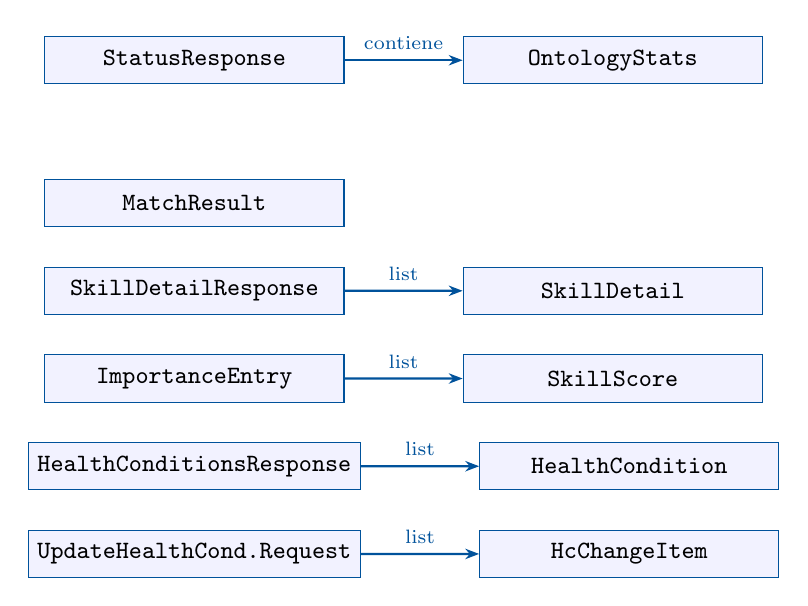
\begin{tikzpicture}[scale=0.85,
  node distance=0.5cm and 1.5cm,
  model/.style={rectangle, draw=rientraBlue, fill=blue!5,
                minimum width=3.8cm, minimum height=0.6cm,
                align=center, font=\ttfamily\small},
  compose/.style={-{Stealth[length=5pt]}, thick, rientraBlue},
  uses/.style={-{Stealth[length=5pt]}, dashed, rientraGray},
]
  % StatusResponse composes OntologyStats
  \node[model] (sr) {StatusResponse};
  \node[model, right=1.5cm of sr] (os) {OntologyStats};
  \draw[compose] (sr) -- (os) node[midway, above, font=\scriptsize] {contiene};

  % MatchResult standalone
  \node[model, below=1.2cm of sr] (mr) {MatchResult};

  % SkillDetailResponse composes SkillDetail
  \node[model, below=0.5cm of mr] (sdr) {SkillDetailResponse};
  \node[model, right=1.5cm of sdr] (sd) {SkillDetail};
  \draw[compose] (sdr) -- (sd) node[midway, above, font=\scriptsize] {list};

  % ImportanceEntry composes SkillScore
  \node[model, below=0.5cm of sdr] (ie) {ImportanceEntry};
  \node[model, right=1.5cm of ie] (ss) {SkillScore};
  \draw[compose] (ie) -- (ss) node[midway, above, font=\scriptsize] {list};

  % HealthConditionsResponse composes HealthCondition
  \node[model, below=0.5cm of ie] (hcr) {HealthConditionsResponse};
  \node[model, right=1.5cm of hcr] (hc) {HealthCondition};
  \draw[compose] (hcr) -- (hc) node[midway, above, font=\scriptsize] {list};

  % UpdateHCRequest composes HcChangeItem
  \node[model, below=0.5cm of hcr] (uhcr) {UpdateHealthCond.Request};
  \node[model, right=1.5cm of uhcr] (hci) {HcChangeItem};
  \draw[compose] (uhcr) -- (hci) node[midway, above, font=\scriptsize] {list};
\end{tikzpicture}%
}% end resizebox
\caption{Relazioni di composizione tra i modelli Pydantic principali.}
\end{figure}

\subsection{Convenzioni adottate nel modulo}

\begin{longtable}{L{4.5cm} L{8cm}}
  \toprule
  \textbf{Convenzione} & \textbf{Motivazione} \\
  \midrule
  \endhead
  Campi stringa con default \texttt{""} anzich\'{e} \texttt{None} &
    Evita \texttt{null} nel JSON per campi che il frontend tratta
    sempre come stringhe (nomi, descrizioni, IRI). \\[4pt]
  Liste con default \texttt{[]} &
    Coerenza: il frontend non deve gestire \texttt{null} vs.\
    lista vuota. In Pydantic v2 le liste di default sono sicure
    (non condivise tra istanze). \\[4pt]
  \texttt{Optional[int]} per i qualificatori &
    I qualificatori ICF possono essere assenti se il codice
    \`{e} presente nell'ontologia senza un valore esplicito. \\[4pt]
  \texttt{Field(\allowbreak description=...)} su tutti i campi non ovvi &
    Popola la documentazione OpenAPI con testo leggibile,
    riducendo la necessit\`{a} di documentazione separata. \\[4pt]
  \texttt{Field(examples=[...])} &
    Fornisce valori di esempio nello schema OpenAPI/Swagger UI,
    facilitando il testing manuale degli endpoint. \\[4pt]
  Nessun \texttt{model\_config} o \texttt{Config} class &
    I default di Pydantic v2 (strict mode off, from\_attributes off)
    sono adeguati; la serializzazione avviene tramite
    \texttt{model\_dump()} esplicito dove necessario. \\
  \bottomrule
\end{longtable}

% ============================================================
\section{Modulo \texttt{reasoner.py} --- Logica semantica e ragionamento}
% ============================================================

\subsection{Ruolo e responsabilit\`{a} del modulo}

\texttt{reasoner.py} \`{e} il \textbf{nucleo computazionale} dell'intero
microservizio. La separazione da \texttt{main.py} \`{e} una scelta architetturale
deliberata: owlready2, Pellet e le query SPARQL non dipendono in alcun modo da
FastAPI, Uvicorn o dal protocollo HTTP. Mantenerli in moduli distinti permette
di testare la logica semantica in isolamento (importando solo \texttt{reasoner.py}
senza avviare il server), di sostituire il framework HTTP in futuro senza
toccare il codice di reasoning, e di ragionare sulla complessit\`{a} dei due
domini (web vs. ontologico) separatamente. Implementa quattro macro-responsabilit\`{a} distinte:

\begin{enumerate}
  \item \textbf{Caricamento e ragionamento ontologico}: carica il file RDF
        in owlready2 ed esegue il reasoner Pellet (DL reasoner con supporto
        SWRL), ottenendo la chiusura inferenziale completa dell'ontologia.
  \item \textbf{Query SPARQL}: espone funzioni pubbliche che interrogano
        l'\texttt{owlready2 default\_world} per restituire dati strutturati
        (workers, jobs, condizioni ICF, risultati di matching).
  \item \textbf{Gestione dello stato del servizio}: mantiene il singleton
        \texttt{ReasonerState} che traccia lo stato del processo di
        caricamento (\texttt{loading} / \texttt{ready} / \texttt{error}).
  \item \textbf{Mutazioni in-memory e persistenza}: applica modifiche alle
        condizioni di salute ICF e agli assegnamenti job, riesegue Pellet,
        e aggiorna sia il file RDF su disco sia la cache locale JSON.
\end{enumerate}

\begin{infobox}[Separazione delle responsabilit\`{a}]
Il modulo \`{e} definito come \textit{pure logic layer}: non dipende da
FastAPI, non esegue output su console (nessun \texttt{print}/Rich/matplotlib)
e non importa \texttt{main.py}. Questo design a bassa dipendenza facilita
il test unitario delle funzioni di reasoning in isolamento rispetto
all'applicazione HTTP.
\end{infobox}

\subsection{Dipendenze e silenziamento dei log}

\begin{lstlisting}[caption={Silencing dei log rumorosi di owlready2 e Java.}]
warnings.filterwarnings("ignore")
logging.disable(logging.WARNING)
owlready2.set_log_level(0)
\end{lstlisting}

owlready2 e la JVM sottostante producono un volume elevato di messaggi
di log (deprecation warning, messaggi di stato di Pellet, eccezioni
catturate internamente). Queste tre righe li sopprimono a livello
globale prima che qualsiasi endpoint possa rispondere, evitando
inquinamento dei log dell'applicazione. Il logging applicativo rimane
disponibile tramite il modulo \texttt{logging} standard.

\subsection{Costanti IRI dell'ontologia Rientr@}

Le propriet\`{a} OWL dell'ontologia Rientr@ vengono referenziate tramite
i loro IRI completi. La scelta di definire queste costanti a livello di
modulo (anzich\'{e} recuperarle dinamicamente a ogni query) serve a:

\begin{itemize}[noitemsep]
  \item Evitare stringhe magiche sparse nel codice.
  \item Centralizzare la manutenzione in caso di cambio del namespace.
  \item Documentare esplicitamente quali propriet\`{a} usa il sistema.
\end{itemize}

\begin{table}[H]
\centering\small
\caption{Costanti IRI principali e loro significato ontologico.}
\begin{tabular}{L{4.5cm} L{8cm}}
\toprule
\textbf{Costante} & \textbf{Propriet\`{a} OWL / Significato} \\
\midrule
\texttt{IRI\_IS\_VERY\_IMP} & \texttt{isVeryImportantFor} --- skill critica per un job (SWRL r. 9) \\
\texttt{IRI\_IS\_IMP}       & \texttt{isImportantFor} --- skill importante (SWRL r. 10) \\
\texttt{IRI\_IS\_SOMEWHAT}  & \texttt{isSomewhat\-ImportantFor} --- skill moderatamente imp. (SWRL r. 11) \\
\texttt{IRI\_IS\_LESS}      & \texttt{isLessImportantFor} --- skill poco importante (SWRL r. 12) \\
\texttt{IRI\_HAS\_CRIT}     & \texttt{hasSpecificCriticality} --- CS inferito da Pellet per coppia (SkAb, Persona) \\
\texttt{IRI\_REQUIRES}      & \texttt{requires} --- relazione Job $\rightarrow$ JobDescEntry \\
\texttt{IRI\_CONCERNS}      & \texttt{concerns} --- relazione JobDescEntry $\rightarrow$ SkAb \\
\texttt{IRI\_HAS\_SCORE}    & \texttt{hasScore} --- punteggio O*NET di un JobDescEntry \\
\texttt{IRI\_IS\_EVAL\_JOB} & \texttt{isEvaluatedForJob} --- Persona valutata per un Job \\
\texttt{IRI\_IS\_IN\_HC}    & \texttt{isInHealthCondition} --- Persona $\rightarrow$ HC \\
\texttt{IRI\_IS\_SELECTED}  & \texttt{isSelected} --- flag di selezione attiva del worker \\
\texttt{IRI\_IS\_TRANSL}    & \texttt{isTranslatedWithICFCode} --- SkAb $\rightarrow$ codice ICF \\
\texttt{IRI\_BFQUAL}        & \texttt{BFqual} --- qualificatore ICF Body Functions/Structures \\
\texttt{IRI\_AP1QUAL}       & \texttt{AP1qual} --- qualificatore ICF Activities \& Participation \\
\texttt{IRI\_FIRST\_NAME}   & \texttt{first\_name} (FOAF) --- nome del lavoratore \\
\texttt{IRI\_SURNAME}       & \texttt{surname} (FOAF) --- cognome del lavoratore \\
\texttt{IRI\_IS\_DESCRIBED\_BY} & \texttt{isDescribedBy} --- HC $\rightarrow$ Descriptor \\
\texttt{IRI\_INVOLVES\_ICF} & \texttt{involvesICFCode} --- Descriptor $\rightarrow$ individuo ICF \\
\texttt{IRI\_ICF\_DESCRIPTION} & \texttt{description} --- testo descrittivo del codice ICF \\
\texttt{IRI\_ONET\_DEFINITION} & \texttt{ONet\_definition} --- definizione testuale O*NET di una SkAb \\
\bottomrule
\end{tabular}
\end{table}

\subsubsection{Soglie di idoneit\`{a} (Fig. 4 del paper)}

\begin{lstlisting}[caption={Costanti per la classificazione di idoneit\`{a}.}]
JS_RED_INTERCEPT    = 21.0   # intercetta soglia NOT SUITABLE
JS_YELLOW_INTERCEPT = 15.5   # intercetta soglia SUITABLE WITH PRECAUTIONS
JS_SLOPE            = -0.5   # pendenza comune delle due rette di soglia
\end{lstlisting}

\noindent Le due rette che delimitano le tre zone del piano GCS\%--AISA\% sono:
\begin{align}
  \text{Soglia rossa (NOT SUITABLE)}   &: \text{GCS} = -0.5 \cdot \text{AISA} + 21.0 \\
  \text{Soglia gialla (PRECAUTIONS)}   &: \text{GCS} = -0.5 \cdot \text{AISA} + 15.5
\end{align}
Un lavoratore con $\text{GCS} > \text{soglia rossa}$ non \`{e} idoneo;
tra le due soglie \`{e} idoneo con precauzioni; sotto la soglia gialla \`{e}
idoneo.

% -----------------------------------------------------------------------------
\subsection{Classe \texttt{ReasonerState} --- Stato globale del servizio}
% -----------------------------------------------------------------------------

\begin{lstlisting}[caption={Classe \texttt{ReasonerState} --- singleton thread-safe.}]
class ReasonerState:
    def __init__(self) -> None:
        self._lock          = threading.Lock()
        self.status         = "loading"
        self.message        = "Ontology not yet loaded."
        self.ontology_path  = ""
        self.elapsed_pellet: Optional[float] = None
        self.stats: dict    = {}
\end{lstlisting}

\noindent \texttt{ReasonerState} \`{e} un singleton a livello di modulo che espone
il ciclo di vita del reasoner agli endpoint FastAPI. Ogni transizione
di stato \`{e} protetta da un \texttt{threading.Lock} per garantire
visibilit\`{a} corretta tra il thread Pellet e i thread dei worker ASGI.

Il lock \`{e} necessario perch\'{e} Python non garantisce l'atomicit\`{a}
dell'assegnamento di attributi di oggetto in un contesto multi-thread:
anche \texttt{self.status = "ready"} non \`{e} atomico in CPython
(coinvolge pi\`{u} bytecode). Senza lock, un thread ASGI potrebbe
leggere \texttt{status = "ready"} mentre \texttt{message} \`{e} ancora
il vecchio valore (\textit{torn read}), producendo risposte JSON
internamente inconsistenti a \texttt{GET /status}.

\begin{table}[H]
\centering
\caption{Metodi di transizione di stato di \texttt{ReasonerState}.}
\begin{tabular}{L{5.8cm} L{6.7cm}}
\toprule
\textbf{Metodo} & \textbf{Transizione / Effetto} \\
\midrule
\texttt{set\_\allowbreak{}ready(path, elapsed, stats)} &
  $\texttt{loading} \rightarrow \texttt{ready}$; registra percorso, tempo
  Pellet e statistiche ontologia. \\[4pt]
\texttt{set\_\allowbreak{}ready\_\allowbreak{}from\_\allowbreak{}cache(path, stats)} &
  $\texttt{loading} \rightarrow \texttt{ready}$ da cache JSON; nessun
  elapsed (Pellet non ha girato). \\[4pt]
\texttt{set\_loading(message)} &
  Forza ritorno a \texttt{loading} durante un re-reasoning
  (es.\ dopo update HC o job). \\[4pt]
\texttt{set\_error(error)} &
  $\texttt{loading} \rightarrow \texttt{error}$; messaggio di errore
  visibile da \texttt{GET /status}. \\[4pt]
\texttt{is\_ready()} &
  Controllo booleano rapido usato dai lock di mutazione. \\
\bottomrule
\end{tabular}
\end{table}

\subsubsection{Variabili globali di modulo}
\vspace{2pt}
\begin{lstlisting}[caption={Variabili globali di stato e cache.}]
state                = ReasonerState()      # singleton esposto a main.py
_selection_lock      = threading.Lock()     # serializza mutazioni isSelected
_icf_core_set_map    : dict[str, list[str]] # ICF code -> [core set labels]
_snapshot_cache      : dict | None          # cache JSON in-memory
_live_reasoner_ready : bool                 # True dopo Pellet completo
_pending_selected_worker_id : Optional[str] # richiesta selezione durante warmup
_loaded_ontology             = None         # oggetto ontologia owlready2
\end{lstlisting}

\noindent Il flag \texttt{\_live\_reasoner\_ready} \`{e} distinto da
\texttt{state.status == "ready"} perch\'{e} lo stato pu\`{o} diventare
\texttt{ready} anche grazie alla snapshot cache, mentre le operazioni
di \textit{mutazione} (update HC, update jobs) richiedono la presenza
dell'ontologia viva in owlready2 --- condizione garantita solo da
\texttt{\_live\_reasoner\_ready = True}.

% -----------------------------------------------------------------------------
\subsection{Funzioni di utilit\`{a}}
% -----------------------------------------------------------------------------

\subsubsection{\texttt{local\_name(entity)}}

\begin{lstlisting}[caption={Estrazione del nome locale da un IRI.}]
def local_name(entity) -> str:
    if hasattr(entity, "name"):
        return entity.name
    s = str(entity)
    return s.split("#")[-1] if "#" in s else s.split("/")[-1]
\end{lstlisting}

\noindent Converte un oggetto owlready2 o una stringa IRI nel suo frammento locale
(es. \texttt{http://...JobList\#Job\_\allowbreak{}Carpenter} $\rightarrow$
\texttt{Job\_Carpenter}). La priorit\`{a} all'attributo \texttt{.name}
di owlready2 \`{e} pi\`{u} efficiente della manipolazione stringa.

\subsubsection{\texttt{criticality\_label(cs)}}

\begin{lstlisting}[caption={Mappatura CS $\rightarrow$ etichetta (Fig. 2 del paper).}]
def criticality_label(cs: int) -> str:
    if   cs >= 7: return "EXTREMELY CRITICAL"
    elif cs >= 5: return "RELEVANTLY CRITICAL"
    elif cs >= 3: return "MODERATELY CRITICAL"
    elif cs >= 1: return "SLIGHTLY CRITICAL"
    else:         return "not critical"
\end{lstlisting}

\noindent Il Criticality Score (CS = qualifier $\times$ anchor) ha range [0, 12].
Le soglie sono definite in Fig. 2 del paper Rientr@ e codificano la
gravit\`{a} dell'impatto di una condizione di salute su una specifica
skill. CS = 0 significa nessun impatto; CS = 12 (qualifier=4, anchor=3)
\`{e} il caso massimo di impatto estremo.

\subsubsection{\texttt{job\_suitability(gcs, aisa)}}

\begin{lstlisting}[caption={Classificazione di idoneit\`{a} per coppia (GCS\%, AISA\%).}]
def job_suitability(gcs: float, aisa: float) -> tuple[str, str]:
    thr_red    = JS_SLOPE * aisa + JS_RED_INTERCEPT    # 21 - 0.5*aisa
    thr_yellow = JS_SLOPE * aisa + JS_YELLOW_INTERCEPT # 15.5 - 0.5*aisa
    if gcs > thr_red:
        label = "NOT SUITABLE"
    elif gcs >= thr_yellow:
        label = "SUITABLE WITH PRECAUTIONS"
    else:
        label = "SUITABLE"
    return label, SUITABILITY_COLORS[label]
\end{lstlisting}

\noindent Restituisce una tupla \texttt{(label, hex\_color)}. La doppia soglia
lineare \`{e} dipendente da AISA\%: al crescere della percentuale di
skill compromesse, la soglia di idoneit\`{a} si abbassa (GCS critico pi\`{u}
basso). Questo modella il fatto che molte compromissioni moderate sono
complessivamente pi\`{u} limitanti di poche compromissioni gravi.

\subsubsection{\texttt{\_score\_to\_anchor(score)}}

\begin{lstlisting}[caption={Conversione punteggio O*NET in anchor [0-3] (Tabella 2 del paper).}]
def _score_to_anchor(score: int) -> int:
    if score >= 75: return 3
    if score >= 50: return 2
    if score >= 26: return 1
    return 0
\end{lstlisting}

\noindent L'anchor \`{e} il fattore moltiplicativo dell'importanza della skill per
un dato job. Il punteggio O*NET (0--100) viene discretizzato in quattro
livelli secondo la Tabella 2 del paper. Questo permette al sistema di
amplificare l'impatto delle skill ad alta importanza nel calcolo del CS.

% -----------------------------------------------------------------------------
\subsection{Sistema di cache snapshot}
% -----------------------------------------------------------------------------

Il sistema di cache \`{e} uno degli aspetti architetturali pi\`{u}
importanti del modulo. Risolve un problema fondamentale: Pellet impiega
30--120 secondi per completare il ragionamento, rendendo inutilizzabile
il servizio al primo avvio.

\subsubsection{Strategia generale}

\begin{figure}[htbp]
\centering
\resizebox{\linewidth}{!}{%
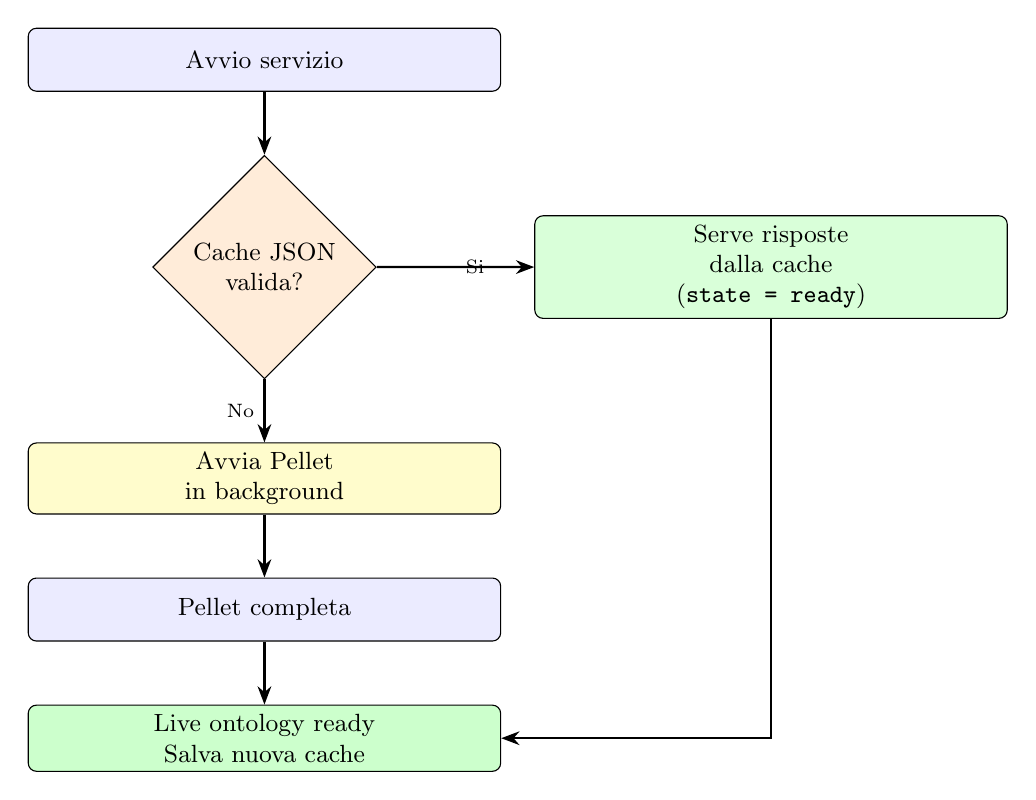
\begin{tikzpicture}[scale=0.85,
  node distance=0.9cm,
  block/.style={rectangle, rounded corners=3pt, draw, fill=blue!8,
                minimum width=6cm, minimum height=0.8cm, align=center, font=\small},
  decision/.style={diamond, draw, fill=orange!15, align=center,
                   font=\small, inner sep=3pt},
  arrow/.style={-{Stealth}, thick},
  yes/.style={font=\scriptsize, right},
  no/.style={font=\scriptsize, below},
]
  \node[block] (start) {Avvio servizio};
  \node[decision, below=0.8cm of start] (cache_exists) {Cache JSON\\valida?};
  \node[block, right=2cm of cache_exists, fill=green!15] (serve_cache)
    {Serve risposte\\dalla cache\\(\texttt{state = ready})};
  \node[block, below=0.8cm of cache_exists, fill=yellow!20] (pellet_start)
    {Avvia Pellet\\in background};
  \node[block, below=0.8cm of pellet_start] (pellet_done) {Pellet completa};
  \node[block, below=0.8cm of pellet_done, fill=green!20] (live_ready)
    {Live ontology ready\\Salva nuova cache};

  \draw[arrow] (start) -- (cache_exists);
  \draw[arrow] (cache_exists) -- node[yes] {Si} (serve_cache);
  \draw[arrow] (cache_exists) -- node[no, left] {No} (pellet_start);
  \draw[arrow] (pellet_start) -- (pellet_done);
  \draw[arrow] (pellet_done) -- (live_ready);
  \draw[arrow] (serve_cache) |- (live_ready);
\end{tikzpicture}%
}% end resizebox
\caption{Strategia di avvio rapido con snapshot cache.}
\end{figure}

\subsubsection{\texttt{\_ontology\_fingerprint(path)}}

\begin{lstlisting}[caption={Fingerprint del file ontologico per invalidazione della cache.}]
def _ontology_fingerprint(path: str) -> str:
    abs_path = os.path.abspath(path)
    stat = os.stat(abs_path)
    payload = f"{abs_path}|{stat.st_size}|{stat.st_mtime_ns}".encode()
    return hashlib.sha256(payload).hexdigest()[:16]
\end{lstlisting}

\noindent Il fingerprint combina percorso assoluto, dimensione e timestamp di
modifica in nanosecondi. L'hash SHA-256 troncato a 16 caratteri \`{e}
sufficientemente unico da evitare collisioni pratiche. Il fingerprint
viene usato come suffisso del nome del file cache:
\texttt{inference\_\{fingerprint\}.json}.

La scelta di non fare hash del contenuto del file (che sarebbe pi\`{u}
affidabile ma molto pi\`{u} lento su file RDF di decine di MB) \`{e}
un compromesso consapevole: il timestamp di modifica cattura il 99.9\%
dei casi reali di cambiamento.

\subsubsection{\texttt{load\_\allowbreak{}snapshot\_\allowbreak{}cache(rdf\_\allowbreak{}path, update\_\allowbreak{}state)}}

Tenta di caricare la cache JSON corrispondente all'ontologia corrente.
Valida che il JSON contenga tutte le chiavi obbligatorie prima di
accettarlo; un file di cache corrotto o incompleto viene semplicemente
ignorato (senza errore), facendo ricadere il sistema sul percorso normale
con Pellet.

\begin{lstlisting}[caption={Chiavi obbligatorie nella snapshot cache.}]
required_keys = {
    "source_hash", "source_path", "stats",
    "workers", "jobs", "core_sets", "icf_codes",
    "health_conditions", "importance_by_job",
    "job_profiles", "match_results_by_worker",
    "skill_details_by_worker_job",
}
\end{lstlisting}

\noindent Il parametro \texttt{update\_state=True} permette di caricare la cache
senza aggiornare il \texttt{ReasonerState} --- utile quando la funzione
viene chiamata internamente dopo un re-reasoning per aggiornare la cache
in-memory senza interferire con lo stato visibile agli endpoint.

\subsubsection{\texttt{\_\allowbreak{}save\_\allowbreak{}snapshot\_\allowbreak{}cache(source\_\allowbreak{}path, elapsed, stats)}}

Questa funzione \`{e} la pi\`{u} onerosa del modulo in termini di
computazione: itera su tutti i worker, seleziona ciascuno temporaneamente
con \texttt{set\_selected\_worker}, esegue tutte le query di matching e
skill detail, poi ripristina la selezione originale. Questo garantisce
che la cache contenga dati precalcolati per ogni combinazione (worker,
job).

La scrittura su disco avviene in modalit\`{a} atomica:
\begin{lstlisting}[caption={Scrittura atomica della cache su disco.}]
tmp_path = f"{cache_path}.tmp"
with open(tmp_path, "w", encoding="utf-8") as fh:
    json.dump(payload, fh, indent=2, ensure_ascii=True)
os.replace(tmp_path, cache_path)  # atomico su POSIX
\end{lstlisting}

\noindent \texttt{os.replace()} \`{e} atomico su filesystem POSIX: se il processo
termina durante la scrittura, il file originale rimane intatto.
\texttt{ensure\_ascii=True} garantisce compatibilit\`{a} con ogni
sistema di file indipendentemente dall'encoding locale.

\subsubsection{\texttt{\_use\_snapshot\_cache()}}

\begin{lstlisting}[caption={Condizione di utilizzo della cache.}]
def _use_snapshot_cache() -> bool:
    return _snapshot_cache is not None and not _live_reasoner_ready
\end{lstlisting}

\noindent La cache viene usata \textbf{solo} finch\'{e} il reasoner live non ha
terminato. Una volta che Pellet completa (\texttt{\_live\_reasoner\_ready
= True}), tutte le query tornano a interrogare direttamente l'ontologia
owlready2, che ha i dati aggiornati dall'inferenza pi\`{u} recente.
Questa transizione avviene automaticamente senza riavvio del servizio.

% -----------------------------------------------------------------------------
\subsection{Fase 1 --- Caricamento dell'ontologia}
% -----------------------------------------------------------------------------

\subsubsection{\texttt{\_find\_rdf\_file()} e \texttt{\_resolve\_rdf\_path()}}

Il percorso del file ontologico viene risolto secondo questa gerarchia
di priorit\`{a}:
\begin{enumerate}[noitemsep]
  \item Argomento esplicito alla funzione.
  \item Variabile d'ambiente \texttt{ONTOLOGY\_PATH}.
  \item Auto-detection: primo file \texttt{.rdf}/\texttt{.owl}/\texttt{.ttl}/\texttt{.n3}
        nella directory del servizio o nella directory padre.
\end{enumerate}
La ricerca si ferma alla prima directory che contiene un candidato
valido, evitando scan inutili.

\subsubsection{\texttt{\_load\_ontology(path)}}

\begin{lstlisting}[caption={Caricamento del file RDF in owlready2.}]
def _load_ontology(path: str):
    abs_path = os.path.abspath(path)
    iri = f"file://{abs_path}"
    buf = io.StringIO()
    with contextlib.redirect_stderr(buf):      # cattura stderr di owlready2
        onto = get_ontology(iri).load()
    return onto
\end{lstlisting}

\noindent Il caricamento usa l'IRI \texttt{file://} anzich\'{e} il percorso nudo
perch\'{e} owlready2 accetta IRI OWL standard come identificatore. Il
\texttt{redirect\_stderr} cattura i messaggi di avviso di owlready2
(es.\ triplo malformata, namespace sconosciuto) senza mostrarli a
console.

% -----------------------------------------------------------------------------
\subsection{Fase 2 --- Esecuzione di Pellet}
% -----------------------------------------------------------------------------

\subsubsection{\texttt{\_run\_pellet(onto)}}

\begin{lstlisting}[caption={Avvio del reasoner Pellet con monkey-patch anti-ciclo.}]
def _run_pellet(onto) -> Optional[float]:
    ThingMeta = type(Thing)
    orig_setattr = ThingMeta.__setattr__

    def patched_setattr(self, name, value):
        if name == "__bases__":
            try:
                orig_setattr(self, name, value)
            except TypeError as exc:
                if "inheritance cycle" not in str(exc):
                    raise     # propaga solo errori non legati a cicli
        else:
            orig_setattr(self, name, value)

    try:
        ThingMeta.__setattr__ = patched_setattr
        with contextlib.redirect_stderr(io.StringIO()) as stderr_buf:
            with onto:
                sync_reasoner_pellet(
                    infer_property_values=True,
                    infer_data_property_values=True,
                )
        ...
    finally:
        ThingMeta.__setattr__ = orig_setattr  # ripristino SEMPRE garantito
\end{lstlisting}

\noindent \begin{infobox}[Monkey-patch per cicli di ereditariet\`{a} ICF]
L'ontologia ICF contiene gerarchie di classi molto profonde (centinaia
di livelli) che Pellet pu\`{o} interpretare come cicli di ereditariet\`{a}
(\textit{inheritance cycle}) durante la materializzazione delle classi
in owlready2. Questo genera una \texttt{TypeError} che interrompe il
ragionamento prima del completamento.

Il monkey-patch sostituisce temporaneamente \texttt{\_\_setattr\_\_} del
metaclasse \texttt{ThingMeta} (la metaclasse di tutte le classi OWL in
owlready2) con una versione che cattura e ignora silenziosamente i
\texttt{TypeError} relativi a cicli, lasciando passare tutti gli altri.
Il blocco \texttt{finally} garantisce che il metaclasse venga sempre
ripristinato, anche in caso di errore, evitando effetti collaterali
su altre parti del codice.

Questa tecnica \`{e} necessaria perch\'{e} owlready2 non espone un
parametro configurabile per questo comportamento.
\end{infobox}

\textbf{Configurazione di Pellet:}
\begin{itemize}[noitemsep]
  \item \texttt{infer\_property\_values=True}: Pellet materializza le
        triple inferite da regole SWRL (es.\ \texttt{isVeryImportantFor},
        \texttt{hasSpecificCriticality}).
  \item \texttt{infer\_\allowbreak{}data\_\allowbreak{}property\_\allowbreak{}values=True}: materializza anche i
        valori di propriet\`{a} dati (es.\ qualificatori numerici inferiti).
\end{itemize}

\textbf{Estrazione del tempo di esecuzione:}
\begin{lstlisting}[caption={Parsing del tempo di esecuzione di Pellet dal log.}]
time_match = re.search(r"Pellet took ([\d.]+)", pellet_log)
return float(time_match.group(1)) if time_match else None
\end{lstlisting}

\noindent Il tempo viene estratto tramite regex dal log di stderr di Pellet
(se presente) e restituito per essere incluso nella risposta
\texttt{GET /status}.

% -----------------------------------------------------------------------------
\subsection{Entry point pubblico --- \texttt{load\_and\_reason()}}
% -----------------------------------------------------------------------------

\begin{lstlisting}[caption={Sequenza completa di \texttt{load\_and\_reason()}.}]
def load_and_reason(rdf_path: str = "") -> None:
    path = _resolve_rdf_path(rdf_path)
    # 1. Caricamento ontologia
    onto = _load_ontology(path)
    _loaded_ontology = onto
    # 2. Ragionamento Pellet
    elapsed = _run_pellet(onto)
    # 3. Statistiche
    stats = {classes, individuals, properties}
    _live_reasoner_ready = True
    # 4. Selezione pending (se arrivata durante il warmup)
    if _pending_selected_worker_id:
        set_selected_worker(_pending_selected_worker_id)
    # 5. Stato pronto
    state.set_ready(path, elapsed, stats)
    # 6. Build mappa ICF -> Core Set
    _build_icf_core_set_map()
    # 7. Salvataggio cache (best-effort)
    _save_snapshot_cache(path, elapsed, stats)
    load_snapshot_cache(path, update_state=False)
\end{lstlisting}

\noindent Il punto 4 gestisce la \textbf{selezione pending}: se durante il warmup
di Pellet il frontend ha chiamato \texttt{POST /workers/select} (quando
era in uso la snapshot cache), la richiesta viene buffered in
\texttt{\_\allowbreak{}pending\_\allowbreak{}selected\_\allowbreak{}worker\_\allowbreak{}id} e applicata all'ontologia live
appena Pellet completa. L'ordine \`{e} critico: la selezione deve avvenire
\textit{prima} di \texttt{state.set\_ready()} (punto 5) perch\'{e} appena
lo stato diventa \texttt{ready}, il frontend potrebbe chiamare immediatamente
\texttt{GET /match/\{workerId\}}, che usa \texttt{FILTER(?selected = true)}.
Se la selezione fosse applicata dopo \texttt{set\_ready}, ci sarebbe una
finestra temporale in cui la query SPARQL restituirebbe risultati del
worker precedente. Questo garantisce la consistenza dello stato.

Il punto 7 \`{e} \textit{best-effort}: se la scrittura della cache
fallisce (es.\ disco pieno, permessi), l'eccezione viene silenziata e
il servizio continua a funzionare normalmente in modalit\`{a} live.

% -----------------------------------------------------------------------------
\subsection{Query SPARQL --- Pattern generale}
% -----------------------------------------------------------------------------

Ogni funzione pubblica di query segue questo pattern strutturato:

\begin{lstlisting}[caption={Pattern comune delle funzioni di query.}]
def get_something(param: str) -> list[dict]:
    # 1) Cache check (se Pellet non ha ancora finito)
    if _use_snapshot_cache():
        return list(cast(dict, _snapshot_cache)["key"])

    # 2) Lookup individuo nell'ontologia (se necessario)
    ind = default_world.search_one(iri=f"*#{param}")
    if ind is None:
        raise KeyError(f"'{param}' not found.")

    # 3) Query SPARQL
    rows = _sparql("""SELECT ...""")

    # 4) Aggregazione e costruzione del risultato
    result = []
    for row in rows:
        result.append({...})

    return sorted(result, key=...)
\end{lstlisting}

\noindent Il lookup \texttt{default\_\allowbreak{}world.search\_\allowbreak{}one(iri="*\#" + id)} usa un
pattern wildcard che corrisponde a qualsiasi IRI il cui frammento locale
\`{e} uguale all'ID, indipendentemente dal namespace. Questo rende le
query robuste a piccole variazioni del namespace tra versioni diverse
dell'ontologia.

% -----------------------------------------------------------------------------
\subsection{Query Q0 --- Workers e Jobs}
% -----------------------------------------------------------------------------

\subsubsection{\texttt{get\_workers()}}

\begin{lstlisting}[caption={SPARQL per la lista dei workers.}]
SELECT DISTINCT ?person WHERE {
    ?person <isEvaluatedForJob> ?job .
}
\end{lstlisting}

\noindent Il filtro \texttt{isEvaluatedForJob} \`{e} intenzionale: l'ontologia pu\`{o}
contenere individui \texttt{FOAF:Person} che non sono ancora stati collegati
ad alcun job (es.\ importati ma non ancora configurati). Restituire queste
persone nella lista produrrebbe elementi non actionable: selezionarli
porterebbe a \texttt{/match} vuoto e a una \texttt{JobAnalysisView} con
errore. Il filtro garantisce che la lista contenga solo worker su cui il
sistema pu\`{o} effettivamente operare.

Per ogni individuo \texttt{Person} trovato, le propriet\`{a}
\texttt{first\_name}, \texttt{surname} e \texttt{isSelected} vengono
recuperate tramite accesso diretto all'oggetto owlready2 (pi\`{u} efficiente
di una seconda query SPARQL). La lista viene ordinata per ID per garantire
output deterministico.

\subsubsection{\texttt{get\_jobs()}}

\begin{lstlisting}[caption={SPARQL per la lista dei job.}]
SELECT DISTINCT ?job WHERE {
    ?job <requires> ?jde .
}
\end{lstlisting}

\noindent Il filtro \texttt{requires} esclude i job ``vuoti'' (senza profilo skill).
Il \texttt{label} viene generato dal local name sostituendo \texttt{\_}
con spazio, senza overhead di query aggiuntive.

% -----------------------------------------------------------------------------
\subsection{Query --- Condizioni di salute ICF}
% -----------------------------------------------------------------------------

\subsubsection{\texttt{get\_\allowbreak{}health\_\allowbreak{}conditions(worker\_\allowbreak{}id)}}

La query naviga la catena ontologica:
\[
\texttt{Person} \xrightarrow{\text{isInHealthCondition}} \texttt{HC}
\xrightarrow{\text{isDescribedBy}} \texttt{Descriptor}
\xrightarrow{\text{involvesICFCode}} \texttt{ICF\_Individual}
\]

\begin{lstlisting}[caption={SPARQL per le condizioni ICF di un worker.}]
SELECT ?icf ?desc ?bfq ?ap1q WHERE {
    <person_iri> <isInHealthCondition> ?hc .
    ?hc  <isDescribedBy>  ?des .
    ?des <involvesICFCode> ?icf .
    OPTIONAL { ?icf <description> ?desc }
    OPTIONAL { ?des <BFqual>  ?bfq  }
    OPTIONAL { ?des <AP1qual> ?ap1q }
}
\end{lstlisting}

\noindent Il local name degli individui ICF nell'ontologia pu\`{o} avere il formato
composto \texttt{b1408-AuditoryAttention}. Il codice gestisce questo
caso con una split sul carattere \texttt{-} e una regex di separazione
CamelCase:
\begin{lstlisting}[caption={Parsing dei compound IRI ICF.}]
icf_code, embedded_name = full_id.split('-', 1)
embedded_name = re.sub(r'(?<=[a-z0-9])(?=[A-Z])', ' ', embedded_name)
# "AuditoryAttention" -> "Auditory Attention"
\end{lstlisting}

\noindent \subsubsection{\texttt{get\_all\_icf\_codes()}}

Restituisce il catalogo completo dei codici ICF per la wizard di
modifica. Quando pi\`{u} individui ontologici si riducono allo stesso
codice puro (es.\ \texttt{b1408-Var1} e \texttt{b1408-Var2} entrambi
codice \texttt{b1408}), vengono \textbf{fusi} in un unico record,
preferendo il primo nome e la prima descrizione non-vuota. Questo
\`{e} necessario perch\'{e} la wizard opera sul codice ICF, non sulle
varianti ontologiche.

La categoria ICF (\textit{Body Functions}, \textit{Activities and
Participation}, \textit{Body Structures}, \textit{Environmental Factors})
viene derivata dal prefisso del codice (b, d, s, e).

% -----------------------------------------------------------------------------
\subsection{Query Q4 --- Importanza skill per job}
% -----------------------------------------------------------------------------

\subsubsection{\texttt{get\_\allowbreak{}importance\_\allowbreak{}summary(job\_\allowbreak{}id)}}

Esegue quattro query SPARQL distinte, una per ogni livello di importanza
SWRL (regole 9--12). Una singola query con \texttt{UNION} sarebbe semanticamente
equivalente ma renderebbe impossibile determinare a quale livello di importanza
appartiene ogni skill senza aggiungere una variabile \texttt{?level} e
un'ulteriore logica di decodifica. Le quattro query separate producono
direttamente strutture dati partizionate per livello, pronte per la
serializzazione in \texttt{ImportanceEntry} senza post-processing:

\begin{lstlisting}[caption={Pattern delle query Q4 per importanza.}]
for label, iri in IMPORTANCE_IRIS.items():
    rows = _sparql(f"""
        SELECT ?skab ?job ?score WHERE {{
            ?skab <{iri}> ?job .        # la skill e' importante per il job
            ?jde  <concerns> ?skab .    # il descriptor riguarda la skill
            ?job  <requires> ?jde .     # il job richiede il descriptor
            ?jde  <hasScore> ?score .   # punteggio O*NET
        }}
    """)
\end{lstlisting}

\noindent Le propriet\`{a} \texttt{isVeryImportantFor}, \texttt{isImportantFor},
ecc.\ sono inferite da Pellet tramite le regole SWRL 9--12. Non esistono
nel file RDF originale ma sono materializzate nell'\texttt{owlready2
default\_world} dopo \texttt{sync\_reasoner\_pellet}. Questa \`{e} la
dimostrazione concreta del valore del reasoning: senza Pellet, queste
propriet\`{a} non esisterebbero e non sarebbe possibile rispondere alla
domanda ``quali skill sono molto importanti per questo job?'' senza
ricalcolare le soglie O*NET a runtime in Python. Con Pellet, la risposta
\`{e} una semplice query SPARQL su triple esistenti.

L'output aggrega le skill per livello di importanza e le ordina per score
decrescente, cos\`{\i} il frontend pu\`{o} mostrarle in ordine di rilevanza.

% -----------------------------------------------------------------------------
\subsection{Query Q1+Q2 --- GCS\% e AISA\%}
% -----------------------------------------------------------------------------

\subsubsection{\texttt{get\_\allowbreak{}match\_\allowbreak{}results(worker\_\allowbreak{}id)}}

La query principale Q1+Q2 \`{e} la pi\`{u} complessa del sistema:

\begin{lstlisting}[caption={SPARQL principale per GCS\% e AISA\% (Q1+Q2).}]
SELECT ?person ?job ?skab ?score ?bfq ?ap1q WHERE {
    ?person <isEvaluatedForJob> ?job .
    ?person <isSelected>        ?selected .
    FILTER(?selected = true)
    ?job    <requires>    ?jde .
    ?jde    <concerns>    ?skab .
    ?jde    <hasScore>    ?score .
    ?skab   <isTranslatedWithICFCode> ?icf .
    ?person <isInHealthCondition>     ?hc .
    ?hc  <isDescribedBy>  ?des .
    ?des <involvesICFCode> ?icf .
    OPTIONAL { ?des <BFqual>  ?bfq  }
    OPTIONAL { ?des <AP1qual> ?ap1q }
}
\end{lstlisting}

\noindent Il \texttt{FILTER(?selected = true)} \`{e} il nodo centrale della query:
seleziona solo i lavoratori marcati come attivi nell'ontologia.
Il join tra \texttt{?skab isTranslatedWithICFCode ?icf} e
\texttt{?des involvesICFCode ?icf} realizza il \textbf{matching semantico}
tra la skill richiesta dal job e la condizione di salute del lavoratore:
due entit\`{a} diverse (una skill e una condizione) sono collegate dal
codice ICF che le descrive entrambe.

\subsubsection{Calcolo aggregato \texttt{\_compute\_metrics(agg)}}

\begin{lstlisting}[caption={Calcolo di GCS\% e AISA\% dall'aggregazione.}]
def _compute_metrics(agg: dict) -> list[dict]:
    for (p_id, j_id), data in sorted(agg.items()):
        cs_values = []
        for s_id, entry in data["skabs"].items():
            anchor = _score_to_anchor(entry["score"])
            cs     = entry["qual"] * anchor          # CS = qualifier x anchor
            cs_values.append(cs)
        n_total  = len(cs_values)
        n_crit   = sum(1 for cs in cs_values if cs > 0)
        sum_norm = sum(cs / 12.0 for cs in cs_values)
        gcs_pct  = (sum_norm / n_total) * 100.0      # GCS%
        aisa_pct = (n_crit  / n_total) * 100.0       # AISA%
        suit, color = job_suitability(gcs_pct, aisa_pct)
\end{lstlisting}

\noindent Le formule implementate sono:
\begin{align}
  CS_i &= \text{qualifier}_i \times \text{anchor}_i \quad \in [0, 12] \\
  \text{GCS\%} &= \frac{\sum_i \widehat{CS}_i}{N} \times 100
               = \frac{\sum_i CS_i / 12}{N} \times 100 \\
  \text{AISA\%} &= \frac{|\{i : CS_i > 0\}|}{N} \times 100
\end{align}
dove $N$ \`{e} il numero totale di skill/abilit\`{a} valutate per la
coppia (worker, job).

Le due metriche misurano aspetti \textit{complementari} della compatibilit\`{a}:
\textbf{GCS\%} misura la \textit{gravit\`{a} media} dell'impatto delle
condizioni di salute sulle skill richieste --- un valore alto significa
che molte skill sono molto compromesse. \textbf{AISA\%} misura la
\textit{diffusione} dell'impatto --- un valore alto significa che molte
skill (anche leggermente) sono interessate.

La normalizzazione $CS_i/12$ in GCS\% \`{e} necessaria per portare tutti
i CS sulla stessa scala [0, 1] prima della media: senza normalizzazione,
una skill con anchor 3 e qualifier 4 (CS=12) peserebbe tre volte una
skill con anchor 1 e qualifier 4 (CS=4), anche se entrambe rappresentano
una limitazione completa per i rispettivi livelli di importanza.

La soglia $CS_i > 0$ in AISA\% \`{e} intenzionalmente inclusiva: anche
un CS=1 (lieve) contribuisce al conteggio. Questo riflette la filosofia
del sistema: qualsiasi impatto, per quanto minore, \`{e} clinicamente
rilevante nel contesto della riabilitazione vocazionale.

\subsubsection{Fallback {\small\texttt{\_match\_results\-\_fallback()}}}

Se la query principale restituisce zero righe (es.\ l'ontologia usa
\texttt{hasSpecificCriticality} direttamente anzich\'{e} i qualificatori
ICF separati), il sistema ricade su una query alternativa che usa
\texttt{hasSpecificCriticality} come sorgente del CS. Questo rende il
codice resiliente a variazioni nella struttura dell'ontologia.

% -----------------------------------------------------------------------------
\subsection{Query Q3 --- Dettaglio skill per coppia (worker, job)}
% -----------------------------------------------------------------------------

\subsubsection{\texttt{get\_\allowbreak{}skill\_\allowbreak{}detail(worker\_\allowbreak{}id, job\_\allowbreak{}id)}}

\begin{lstlisting}[caption={SPARQL Q3 per il dettaglio skill.}]
SELECT ?skab ?cs ?score ?def WHERE {
    ?skab <hasSpecificCriticality> ?cs .
    ?jde  <concerns>   ?skab .
    <job_iri> <requires> ?jde .
    ?jde  <hasScore>  ?score .
    <person_iri> <isEvaluatedForJob> <job_iri> .
    OPTIONAL { ?skab <ONet_definition> ?def . }
}
\end{lstlisting}

\noindent Usa \texttt{hasSpecificCriticality} (propriet\`{a} inferita da Pellet
per coppia SkAb--Persona) come sorgente del CS, ricostruendo
\texttt{anchor} e \texttt{qualifier} dalla formula inversa:
\[
\text{qualifier} = \frac{CS}{\text{anchor}} \quad
(\text{anchor} = \texttt{\_score\_to\_anchor(score)})
\]

Il risultato include anche la definizione testuale O*NET della skill
(\texttt{ONet\_definition}), che nel frontend \`{e} mostrata come tooltip
o testo descrittivo nella tabella di dettaglio.

La deduplicazione usa la strategia \textit{keep highest CS}: se la stessa
skill appare pi\`{u} volte con CS diversi (possibile per individui ICF
multipli), viene mantenuta solo la riga con CS massimo.

% -----------------------------------------------------------------------------
\subsection{Mutazione --- Selezione del worker (\texttt{set\_selected\_worker})}
% -----------------------------------------------------------------------------

\begin{lstlisting}[caption={Mutazione atomica di \texttt{isSelected}.}]
def set_selected_worker(worker_id: str) -> dict:
    # Path: cache mode (Pellet non ancora pronto)
    if _use_snapshot_cache():
        ...  # aggiorna _snapshot_cache["workers"][*]["is_selected"]
        _pending_selected_worker_id = worker_id
        return {"previous": old_id, "selected": worker_id}

    # Path: live mode
    sel_prop = default_world.search_one(iri=IRI_IS_SELECTED)
    with _selection_lock:
        # 1. Deseleziona tutti
        for ind in default_world.individuals():
            if sel_prop[ind] and bool(sel_prop[ind][0]):
                old_id = local_name(ind)
                sel_prop[ind] = [False]
        # 2. Seleziona il target
        sel_prop[target] = [True]
    return {"previous": old_id, "selected": worker_id}
\end{lstlisting}

\noindent Il lock \texttt{\_selection\_lock} garantisce che due richieste concorrenti
non possano lasciare l'ontologia con due worker selezionati
contemporaneamente. Il pattern deseleziona-tutti-poi-seleziona-uno
\`{e} O(N\_individui) ma necessario perch\'{e} owlready2 non espone
un indice inverso per la propriet\`{a} \texttt{isSelected}.

In \textbf{cache mode} (durante il warmup), la selezione viene applicata
alla cache in-memory \textit{e} memorizzata in
\texttt{\_\allowbreak{}pending\_\allowbreak{}selected\_\allowbreak{}worker\_\allowbreak{}id} per essere applicata
all'ontologia live quando Pellet completa.

% -----------------------------------------------------------------------------
\subsection{Mutazione --- Aggiornamento condizioni ICF}
% -----------------------------------------------------------------------------

\subsubsection{Struttura del grafo HC nell'ontologia}

\begin{figure}[htbp]
\centering
\resizebox{\linewidth}{!}{%
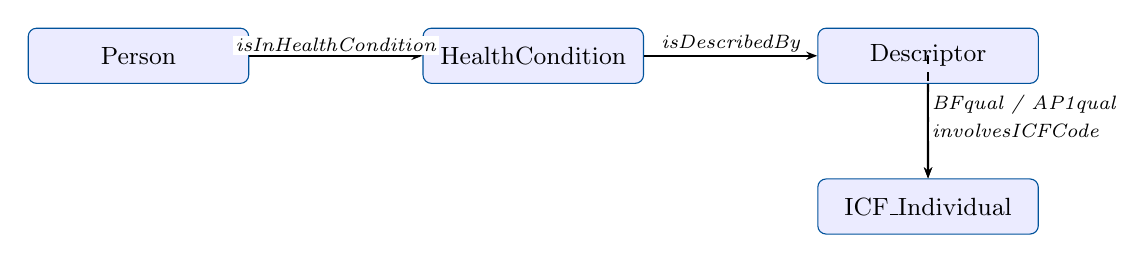
\begin{tikzpicture}[scale=0.85,
  node distance=1cm and 1.5cm,
  ent/.style={rectangle, draw=rientraBlue, fill=blue!8, rounded corners=3pt,
              minimum width=2.8cm, minimum height=0.7cm, align=center, font=\small},
  prop/.style={font=\scriptsize\itshape, above, rientraGray},
  arrow/.style={-{Stealth[length=4pt]}, thick},
]
  \node[ent] (person) {Person};
  \node[ent, right=2.2cm of person] (hc) {HealthCondition};
  \node[ent, right=2.2cm of hc] (des) {Descriptor};
  \node[ent, below=1.2cm of des] (icf) {ICF\_Individual};

  \draw[arrow] (person) -- node[above, font=\scriptsize\itshape, fill=white, inner sep=1pt]
    {isInHealthCondition} (hc);
  \draw[arrow] (hc) -- node[above, font=\scriptsize\itshape, fill=white, inner sep=1pt]
    {isDescribedBy} (des);
  \draw[arrow] (des) -- node[right, font=\scriptsize\itshape, fill=white, inner sep=1pt]
    {involvesICFCode} (icf);
  \draw[arrow, dashed] (des) -|
    node[pos=0.7, right, font=\scriptsize\itshape, fill=white, inner sep=1pt]
    {BFqual / AP1qual} (icf);
\end{tikzpicture}%
}% end resizebox
\caption{Struttura del sottografo HC nell'ontologia Rientr@.}
\end{figure}

\subsubsection{\texttt{\_\allowbreak{}safe\_\allowbreak{}set\_\allowbreak{}prop(prop, ind, value)}}

\begin{lstlisting}[caption={Assegnazione sicura di propriet\`{a} funzionali in owlready2.}]
def _safe_set_prop(prop, ind, value: int | None) -> None:
    prop[ind] = []           # 1. flush tutti i triple esistenti
    if value is not None:
        prop[ind] = [value]  # 2. assegna il nuovo valore
\end{lstlisting}

\noindent \begin{warningbox}[Bug owlready2 --- Propriet\`{a} funzionali]
owlready2 non svuota automaticamente i triple esistenti quando si
assegna \texttt{prop[ind] = [new\_value]} su un individuo che ha gi\`{a}
un valore per quella propriet\`{a}. Il risultato \`{e} la coesistenza di
due triple per la stessa propriet\`{a} funzionale (\texttt{BFqual} o
\texttt{AP1qual}), che causa una \texttt{InconsistentOntologyException}
in Pellet alla successiva esecuzione.

La soluzione adottata \`{e} il flush esplicito \texttt{prop[ind] = []}
prima di ogni assegnazione, che rimuove tutti i triple esistenti.
\end{warningbox}

\subsubsection{Logica delle tre azioni (ADD / REMOVE / MODIFY)}

\paragraph{ADD}
\begin{enumerate}[noitemsep]
  \item Risolve l'individuo ICF dalla cache o dall'ontologia.
  \item Se il codice \`{e} gi\`{a} presente nel profilo HC del worker,
        lo tratta come \textbf{MODIFY} (idempotenza).
  \item Crea un nuovo individuo \texttt{Descriptor}.
  \item Imposta \texttt{involvesICFCode}, \texttt{BFqual} o \texttt{AP1qual}.
  \item Se il worker non ha ancora una \texttt{HealthCondition}, ne crea una nuova.
\end{enumerate}

\paragraph{REMOVE}
\begin{enumerate}[noitemsep]
  \item Localizza il \texttt{Descriptor} corrispondente.
  \item Lo rimuove dalla lista \texttt{isDescribedBy} dell'HC.
  \item Chiama \texttt{owlready2.destroy\_entity()} per rimuovere tutti i
        triple del descriptor dal grafo.
  \item Se l'HC rimane senza descriptor, viene anch'essa distrutta
        e scollegata dal worker (pulizia del ciclo di vita HC).
\end{enumerate}

\paragraph{MODIFY}
\begin{enumerate}[noitemsep]
  \item Localizza il \texttt{Descriptor} corrispondente.
  \item Aggiorna \texttt{BFqual} o \texttt{AP1qual} (in base al prefisso del codice)
        tramite \texttt{\_safe\_set\_prop}.
  \item Azzera l'altra propriet\`{a} per evitare stale data.
\end{enumerate}

\subsubsection{Routing BFqual / AP1qual}
\vspace{2pt}
\begin{lstlisting}[caption={Routing del qualificatore in base al prefisso ICF.}]
def _is_ap1_code(icf_code: str) -> bool:
    return icf_code.lower().startswith("d")

# Uso:
use_ap1    = _is_ap1_code(icf_code)
q_prop     = ap1qual_prop if use_ap1 else bfqual_prop
other_prop = bfqual_prop  if use_ap1 else ap1qual_prop
\end{lstlisting}

\noindent I codici \texttt{d*} (Activities \& Participation) usano \texttt{AP1qual};
tutti gli altri (\texttt{b*}, \texttt{s*}, \texttt{e*}) usano \texttt{BFqual}.
Questa distinzione rispecchia la struttura del sistema ICF, in cui
attivit\`{a}/partecipazione ha un qualificatore separato rispetto alle
funzioni corporee.

% -----------------------------------------------------------------------------
\subsection{Mutazione --- Aggiornamento job assegnati}
% -----------------------------------------------------------------------------

\subsubsection{\texttt{update\_\allowbreak{}worker\_\allowbreak{}jobs(worker\_\allowbreak{}id, job\_\allowbreak{}ids)}}

\begin{lstlisting}[caption={Sostituzione atomica dei link isEvaluatedForJob.}]
def update_worker_jobs(worker_id: str, job_ids: list[str]) -> dict:
    ...
    with _job_lock:
        previous = [local_name(j) for j in (eval_prop[person_ind] or [])]
        # Risolvi job IDs -> individui owlready2
        resolved, unresolved = [], []
        for jid in job_ids:
            ind = default_world.search_one(iri="*#" + jid)
            if ind: resolved.append(ind)
            else:   unresolved.append(jid)
        # Sostituisce atomicamente
        eval_prop[person_ind] = resolved
    _refresh_reasoning_artifacts()
\end{lstlisting}

\noindent \texttt{\_job\_lock} \`{e} un lock \textbf{separato} da
\texttt{\_selection\_lock} perch\'{e} le due mutazioni non hanno conflitti
di risorsa tra loro: \texttt{\_selection\_lock} protegge la propriet\`{a}
\texttt{isSelected} su tutti gli individui, mentre \texttt{\_job\_lock}
protegge \texttt{isEvaluatedForJob} su un singolo individuo. Usare un
unico lock globale serializzerebbe operazioni che potrebbero coesistere
in sicurezza (selezione di un worker mentre si aggiornano i job di un
altro), riducendo inutilmente il throughput in scenari multi-utente.
\texttt{\_job\_lock} serializza le mutazioni degli assegnamenti job.
Dopo la sostituzione atomica in-memory, \texttt{\_\allowbreak{}refresh\_\allowbreak{}reasoning\_\allowbreak{}artifacts()}
esegue la pipeline completa: salva il file RDF, riesegue Pellet,
ricalcola la mappa ICF core set, aggiorna le statistiche e sovrascrive
la cache JSON.

% -----------------------------------------------------------------------------
\subsection{\texttt{\_\allowbreak{}refresh\_\allowbreak{}reasoning\_\allowbreak{}artifacts()} --- Pipeline di re-reasoning}
% -----------------------------------------------------------------------------

\begin{lstlisting}[caption={Sequenza di re-reasoning dopo una mutazione.}]
def _refresh_reasoning_artifacts() -> None:
    state.set_loading("Applying changes and recomputing inference...")
    _live_reasoner_ready = False
    _snapshot_cache = None
    try:
        _save_live_ontology(ontology_path)     # 1. Salva RDF su disco
        elapsed = _run_pellet(_loaded_ontology) # 2. Riesegue Pellet
        _build_icf_core_set_map()               # 3. Ricostruisce mappa ICF
        _build_icf_ind_cache()                  # 4. Ricostruisce cache ICF ind.
        stats = {classes, individuals, properties}
        _live_reasoner_ready = True
        state.set_ready(...)                    # 5. Stato pronto
        _save_snapshot_cache(...)               # 6. Salva nuova cache
        load_snapshot_cache(..., update_state=False)  # 7. Ricarica cache
    except Exception as exc:
        state.set_error(str(exc))
        raise
\end{lstlisting}

\noindent Durante il re-reasoning (passi 1--5), il servizio torna temporaneamente
a stato \texttt{loading}: gli endpoint restituiranno 503 fino al
completamento. Questo garantisce che nessun client riceva dati stale
durante il re-reasoning.

% -----------------------------------------------------------------------------
\subsection{\texttt{inject\_imported\_workers()} --- Integrazione post-import}
% -----------------------------------------------------------------------------

\begin{lstlisting}[caption={Flusso di \texttt{inject\_imported\_workers()}.}]
def inject_imported_workers(new_person_ids, ontology_path) -> dict:
    # 1. Usa rdflib (non owlready2) per leggere l'RDF aggiornato
    g = Graph()
    g.parse(ontology_path, format="xml")

    for person_id in new_person_ids:
        # 2. Cerca l'individuo nel live owlready2
        person_ind = default_world.search_one(iri=str(person_iri))

        # 3. Inietta isEvaluatedForJob dal file aggiornato
        new_jobs = [owlready2_ind for iri in g.objects(person_iri, EVAL_PROP)]
        eval_prop[person_ind] = existing + new_jobs

        # 4. Imposta isSelected = false
        sel_prop[person_ind] = [False]

    # 5. Aggiorna snapshot cache
    _save_snapshot_cache(...)
    load_snapshot_cache(..., update_state=False)
\end{lstlisting}

\noindent \begin{infobox}[Uso di rdflib per la lettura post-import]
L'import SQL scrive nuovi individui nel file RDF su disco, ma il grafo
owlready2 in memoria non viene aggiornato automaticamente. Rieseguire
Pellet (operazione da 30--120 s) solo per leggere i nuovi link
\texttt{isEvaluatedForJob} sarebbe eccessivo.

La soluzione adottata usa \texttt{rdflib} --- una libreria Python per
la lettura di grafi RDF --- per estrarre solo i triple rilevanti dal
file aggiornato, e li inietta direttamente nell'oggetto owlready2 in
memoria. Questo approccio ibrido (rdflib per la lettura, owlready2 per
la scrittura live) permette di aggiornare il grafo in pochi millisecondi
senza un re-reasoning completo.
\end{infobox}

% -----------------------------------------------------------------------------
\subsection{Mappa ICF $\rightarrow$ Core Set}
% -----------------------------------------------------------------------------

\subsubsection{{\small\texttt{\_build\_icf\_\allowbreak{}core\_set\_map()}}}

\begin{lstlisting}[caption={SPARQL per la mappa ICF code $\rightarrow$ Core Set.}]
SELECT DISTINCT ?icf ?coreset WHERE {
    ?icf <rdfs:subClassOf>+ ?coreset .
    ?coreset <rdfs:subClassOf> <ICF_Core_set> .
}
\end{lstlisting}

\noindent Il \texttt{+} nella propriet\`{a} \texttt{rdfs:subClassOf+} indica la
chiusura transitiva: recupera l'appartenenza indiretta anche attraverso
gerarchie di classi profonde. La mappa risultante associa il codice ICF
locale (es.\ \texttt{b1408}) alla lista ordinata dei core set di
appartenenza (es.\ \texttt{["Hearing Loss", "Stroke"]}).

Questa mappa viene costruita \textbf{una sola volta} dopo Pellet, invece
di eseguire la query \texttt{rdfs:subClassOf+} ad ogni chiamata di endpoint.
La motivazione \`{e} prestazionale: la chiusura transitiva di
\texttt{rdfs:subClassOf} su ontologie ICF di grandi dimensioni richiede
una traversata ricorsiva del grafo che pu\`{o} costare centinaia di
millisecondi. Eseguirla a runtime per ogni chiamata di
\texttt{GET /health-conditions/\{id\}} (che pu\`{o} essere chiamata
decine di volte durante una sessione) sarebbe inaccettabile. Il costo
del calcolo una-tantum \`{e} ammortizzato su tutte le richieste successive,
riutilizzata da tutte le query successive (\texttt{get\_health\_conditions},
\texttt{get\_all\_icf\_codes}), eliminando migliaia di query SPARQL
ripetute a runtime.

% -----------------------------------------------------------------------------
\subsection{Concorrenza e thread safety}
% -----------------------------------------------------------------------------

\begin{table}[H]
\centering
\caption{Lock di concorrenza e risorse protette.}
\begin{tabular}{L{4cm} L{4cm} L{4.5cm}}
\toprule
\textbf{Lock} & \textbf{Risorsa protetta} & \textbf{Motivazione} \\
\midrule
\texttt{State.\_lock} &
  Campi \texttt{status}, \texttt{message}, \texttt{stats} &
  Visibilit\`{a} corretta tra thread Pellet e thread ASGI. \\[4pt]
\texttt{\_selection\_lock} &
  Propriet\`{a} \texttt{isSelected} in owlready2 &
  Evita doppia selezione con richieste concorrenti. \\[4pt]
\texttt{\_hc\_lock} &
  Mutazioni di Descriptor/HC &
  Atomicit\`{a} del batch di modifiche ICF. \\[4pt]
\texttt{\_job\_lock} &
  Propriet\`{a} \texttt{isEvaluatedForJob} &
  Sostituzione atomica dei job assegnati. \\
\bottomrule
\end{tabular}
\end{table}

Le query di lettura SPARQL (\texttt{get\_workers}, \texttt{get\_match\_results},
ecc.) non usano lock perch\'{e} operano su strutture dati immutabili
dopo che Pellet ha completato (il grafo owlready2 non viene modificato
durante le letture normali).

% -----------------------------------------------------------------------------
\subsection{Flusso dati completo --- Dalla query al JSON}
% -----------------------------------------------------------------------------

\begin{figure}[htbp]
\centering
\resizebox{\linewidth}{!}{%
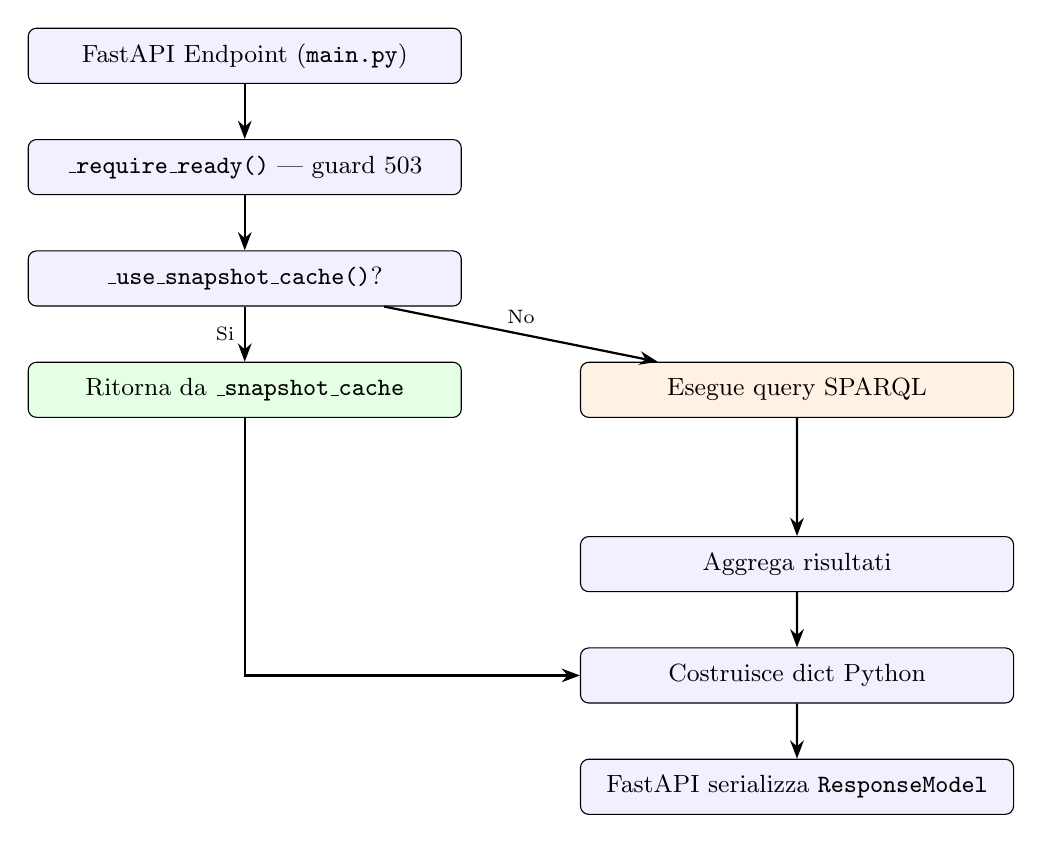
\begin{tikzpicture}[scale=0.85,
  node distance=0.7cm,
  box/.style={rectangle, rounded corners=3pt, draw, fill=blue!6,
              minimum width=5.5cm, minimum height=0.7cm, align=center, font=\small},
  arrow/.style={-{Stealth}, thick},
]
  \node[box] (ep) {FastAPI Endpoint (\texttt{main.py})};
  \node[box, below=of ep] (guard) {\texttt{\_require\_ready()} --- guard 503};
  \node[box, below=of guard] (cache) {\texttt{\_use\_snapshot\_cache()}?};
  \node[box, below=of cache, fill=green!10] (snap) {Ritorna da \texttt{\_snapshot\_cache}};
  \node[box, right=1.5cm of snap, fill=orange!10] (sparql) {Esegue query SPARQL};
  \node[box, below=1.5cm of sparql] (agg) {Aggrega risultati};
  \node[box, below=of agg] (json) {Costruisce dict Python};
  \node[box, below=of json] (resp) {FastAPI serializza \texttt{ResponseModel}};

  \draw[arrow] (ep) -- (guard);
  \draw[arrow] (guard) -- (cache);
  \draw[arrow] (cache) -- node[left, font=\scriptsize] {Si} (snap);
  \draw[arrow] (cache) -- node[above, font=\scriptsize] {No} (sparql);
  \draw[arrow] (sparql) -- (agg);
  \draw[arrow] (agg) -- (json);
  \draw[arrow] (snap) |- (json);
  \draw[arrow] (json) -- (resp);
\end{tikzpicture}%
}% end resizebox
\caption{Flusso dati da endpoint a risposta JSON, con cache bypass.}
\end{figure}

% ============================================================
\section{Ontologia Rientr@ --- Struttura e contenuto}
% ============================================================

\subsection{Panoramica dell'ontologia}

L'ontologia Rientr@ \`{e} un'ontologia OWL~2 DL sviluppata da
\textbf{STIIMA-CNR} (Istituto di Sistemi e Tecnologie Industriali
Intelligenti per il Manifatturiero Avanzato del CNR). Il file RDF
analizzato (\texttt{Rientra.rdf}) corrisponde alla versione
\textbf{3.1}, con ultima revisione al \textbf{30 aprile 2024}.

L'ontologia \`{e} una \textit{box} composita che importa e integra
sette sotto-ontologie distinte, ciascuna con un namespace dedicato:

\begin{table}[H]
\centering
\caption{Sotto-ontologie e namespace dell'ontologia Rientr@ v3.1.}
\begin{tabular}{L{3.5cm} L{5cm} L{4cm}}
\toprule
\textbf{Prefisso XML} & \textbf{IRI base} & \textbf{Contenuto} \\
\midrule
\texttt{Rien3} (\texttt{RientraHC}) &
  \texttt{stiima.cnr.it/\allowbreak RientraHC} &
  Modello condizioni di salute (HC, Descriptor) \\[3pt]
\texttt{FOAF} &
  \texttt{stiima.cnr.it/\allowbreak FOAF-excerpt} &
  Estratto FOAF per la descrizione delle persone \\[3pt]
\texttt{ICF-} &
  \texttt{stiima.cnr.it/\allowbreak ICF-exc-coreset} &
  Estratto ICF con core set (4 originali + 4 aggiuntivi) \\[3pt]
\texttt{JobL} &
  \texttt{stiima.cnr.it/\allowbreak JobList} &
  Lista dei profili lavorativi \\[3pt]
\texttt{SkAb} &
  \texttt{stiima.cnr.it/\allowbreak SkAb} &
  Skills e Abilities da O*NET \\[3pt]
\texttt{JobD} &
  \texttt{stiima.cnr.it/\allowbreak JobDescription} &
  Descrizione job (Job Descriptor con score O*NET) \\[3pt]
\texttt{Rien2} &
  \texttt{stiima.cnr.it/\allowbreak RientraOnt3Merged} &
  Core set aggiuntivi (Hearing Loss, Low Back Pain, ecc.) \\
\bottomrule
\end{tabular}
\end{table}

\subsection{Statistiche degli individui}

Il file RDF contiene \textbf{1.458 individui nominati} distribuiti come segue:

\begin{table}[H]
\centering
\caption{Distribuzione degli individui OWL per namespace.}
\begin{tabular}{L{5cm} C{2.5cm} L{5cm}}
\toprule
\textbf{Namespace} & \textbf{Individui} & \textbf{Tipo di entit\`{a}} \\
\midrule
\texttt{JobList} & 971 & Job e Job\_Descriptor (profili O*NET) \\
\texttt{RientraHC} & 445 & HC, Descriptor, Person istanze \\
\texttt{ICF-exc-coreset} & 26 & Codici ICF nominati nel core set \\
\texttt{Person-CommonBox} & 10 & Individui Person (lavoratori campione) \\
\texttt{SkAb} & 5 & Radici Skills/Abilities \\
\texttt{RientraOnt3} & 1 & Individuo Match \\
\midrule
\textbf{Totale} & \textbf{1.458} & \\
\bottomrule
\end{tabular}
\end{table}

\subsection{Classi principali}

\begin{table}[H]
\centering
\caption{Classi OWL principali dell'ontologia.}
\begin{tabular}{L{5.5cm} L{7cm}}
\toprule
\textbf{Classe} & \textbf{Significato} \\
\midrule
\texttt{FOAF:Person} & Individuo lavoratore con nome, cognome e dati anagrafici \\
{\footnotesize\texttt{FOAF:Person\_with\_impairment}} & Sottoclasse di Person per lavoratori con disabilit\`{a} \\
\texttt{RientraHC:Health\_Condition} & Condizione di salute complessiva di un lavoratore \\
\texttt{RientraHC:Health\_\allowbreak{}Condition\_\allowbreak{}with\_\allowbreak{}impairment} & HC specifica per condizioni con menomazione \\
\texttt{RientraHC:HC\_Descriptor} & Singola voce ICF con qualificatori nella HC \\
\texttt{ICF:ICF} & Classe radice dei codici ICF nell'ontologia \\
\texttt{ICF:Activities\_\allowbreak{}and\_\allowbreak{}participation} & Codici ICF di tipo ``d'' \\
\texttt{ICF:Body\_functions} & Codici ICF di tipo ``b'' \\
\texttt{ICF:Body\_structures} & Codici ICF di tipo ``s'' \\
\texttt{ICF:ICF\_Core\_set} & Classe radice dei core set ICF \\
\texttt{JobList:Job} & Profilo lavorativo (es.\ Assembly Worker) \\
\texttt{JobList:Job\_Descriptor} & Coppia (SkAb, score O*NET) per un Job \\
\texttt{SkAb:Skills} & Competenze trasversali da O*NET \\
\texttt{SkAb:Abilities} & Capacit\`{a} individuali da O*NET \\
\texttt{RientraOnt3:Match} & Classe ausiliaria per il matching (legacy) \\
\bottomrule
\end{tabular}
\end{table}

\subsection{ICF Core Set inclusi}

L'ontologia include estratti ICF organizzati in \textbf{8 core set}
clinicamente rilevanti per la riabilitazione vocazionale:

\begin{table}[H]
\centering
\caption{ICF Core Set presenti nell'ontologia Rientr@ v3.1.}
\begin{tabular}{L{6cm} L{6.5cm}}
\toprule
\textbf{Core Set} & \textbf{Note} \\
\midrule
Spinal Cord Injury (Long Term) & Core set originale ICF \\
Stroke & Core set originale ICF \\
Traumatic Brain Injury & Core set originale ICF \\
Vocational Rehabilitation & Core set originale ICF \\
Hearing Loss & Aggiunto in Rientr@ (\texttt{RientraOnt3Merged}) \\
Low Back Pain & Aggiunto in Rientr@ (\texttt{RientraOnt3Merged}) \\
Musculoskeletal Conditions (Post-Acute Care) & Aggiunto in Rientr@ \\
Hand Conditions & Aggiunto in Rientr@ \\
\bottomrule
\end{tabular}
\end{table}

\subsection{Propriet\`{a} OWL}

\subsubsection{Propriet\`{a} oggetto (Object Properties)}

L'ontologia definisce 25 propriet\`{a} oggetto. Le pi\`{u} rilevanti
per il ragionamento sono:

\begin{table}[H]
\centering\small
\caption{Object Properties chiave dell'ontologia.}
\begin{tabular}{L{5cm} L{3.5cm} L{4cm}}
\toprule
\textbf{Propriet\`{a}} & \textbf{Dominio} & \textbf{Range} \\
\midrule
\texttt{isEvaluatedForJob} & Person & Job \\
\texttt{isInHealthCondition} & Person & Health\_Condition \\
\texttt{isDescribedBy} & Health\_Condition & HC\_Descriptor \\
\texttt{involvesICFCode} & HC\_Descriptor & ICF \\
\texttt{requires} & Job & Job\_Descriptor \\
\texttt{concerns} (funzionale) & Job\_Descriptor & Skills $\cup$ Abilities \\
\texttt{isTranslatedWithICFCode} & Skills $\cup$ Abilities & ICF \\
\texttt{isVeryImportantFor} & Skills $\cup$ Abilities & Job \\
\texttt{isImportantFor} & Skills $\cup$ Abilities & Job \\
\texttt{isSomewhat\-ImportantFor} & Skills $\cup$ Abilities & Job \\
\texttt{isLessImportantFor} & Skills $\cup$ Abilities & Job \\
\texttt{matchedJob} & Person & Job \\
\bottomrule
\end{tabular}
\end{table}

La propriet\`{a} \texttt{concerns} \`{e} dichiarata \textbf{funzionale}:
ogni Job\_Descriptor descrive esattamente una Skill o Ability, garantendo
che il grafo dei requisiti di un job sia una struttura senza ambiguit\`{a}.

\subsubsection{Propriet\`{a} dato (Datatype Properties)}

L'ontologia definisce 20 datatype properties. Quelle usate attivamente
dal microservizio sono:

\begin{table}[H]
\centering
\caption{Datatype Properties rilevanti per il microservizio.}
\begin{tabular}{L{5cm} L{2.5cm} L{5cm}}
\toprule
\textbf{Propriet\`{a}} & \textbf{Tipo XSD} & \textbf{Uso} \\
\midrule
\texttt{first\_name} & \texttt{string} & Nome del lavoratore (FOAF) \\
\texttt{surname} & \texttt{string} & Cognome del lavoratore (FOAF) \\
\texttt{hasScore} & \texttt{integer} & Punteggio O*NET [0--100] del Job\_Descriptor \\
\texttt{BFqual} & \texttt{integer} & Qualificatore ICF Body Functions/Structures [0--4] \\
\texttt{AP1qual} & \texttt{integer} & Qualificatore ICF Activities \& Participation [0--4] \\
\texttt{hasSpecificCriticality} & \texttt{integer} & CS inferito da Pellet per coppia (SkAb, Person) \\
\texttt{isSelected} & \texttt{boolean} & Flag di selezione attiva del worker \\
\texttt{selectedJob} & \texttt{boolean} & Flag job selezionato (legacy, non usato dal svc) \\
\bottomrule
\end{tabular}
\end{table}

Le propriet\`{a} \texttt{AP2qual}, \texttt{AP3qual}, \texttt{AP4qual},
\texttt{BS1qual}, \texttt{BS2qual}, \texttt{BS3qual} sono presenti nell'ontologia
ma non sono al momento utilizzate dal microservizio (previste per
estensioni future del modello ICF).

\subsection{Regole SWRL}

L'ontologia contiene \textbf{13 regole SWRL} che costituiscono il cuore
inferenziale del sistema. La scelta di usare SWRL invece di codice Python
per il calcolo del CS ha due motivazioni fondamentali: (1) le regole
vivono nell'\textit{ontologia}, non nel codice --- un ontology engineer
pu\`{o} modificarle in Prot\'{e}g\'{e} senza toccare Python; (2) Pellet
garantisce la consistenza logica delle regole tramite il ragionamento DL,
rilevando contraddizioni che codice imperativo non individuerebbe.

Le 13 regole sono \textbf{separate} (non una sola con condizioni complesse)
perch\'{e} SWRL non supporta costrutti condizionali
(\texttt{if/else}) nella testa delle regole: ogni regola ha esattamente
una conclusione. La ramificazione logica (prefisso ICF, livello di importanza)
viene espressa moltiplicando le regole. Si dividono in due famiglie:

\subsubsection{Famiglia A --- Calcolo del Criticality Score (regole 1--9)}

Queste 9 regole calcolano \texttt{hasSpecificCriticality} (CS) per ogni
coppia (SkAb, Person) rispetto al job selezionato. La struttura generale
\`{e}:

\begin{multline*}
\text{Persona}(p) \wedge \text{isSelected}(p, \text{true}) \wedge
\text{isEvaluatedForJob}(p, j) \wedge \ldots \wedge \text{multiply}(q, a, \text{cs}) \\
\Rightarrow \text{hasSpecificCriticality}(\text{skab}, \text{cs})
\end{multline*}

dove $q$ \`{e} il qualificatore ICF e $a$ \`{e} l'anchor di importanza
(valore fisso per ogni livello). Le regole si differenziano per:
\begin{itemize}[noitemsep]
  \item \textbf{Tipo di qualificatore}: \texttt{BFqual} (regole 3, 5, 7, 9) vs.\
        \texttt{AP1qual} (regole 2, 4, 6, 8) --- routing b/d ICF.
  \item \textbf{Livello di importanza}: \texttt{isImportantFor} (r.2--3),
        \texttt{isLessImportantFor} (r.4--5), \texttt{isSomewhat\-ImportantFor}
        (r.6--7), \texttt{isVeryImportantFor} (r.8--9).
  \item \textbf{Regola 1}: crea l'individuo \texttt{Match} associando
        \texttt{Person} a \texttt{Job} tramite \texttt{matchedJob} (struttura legacy).
\end{itemize}

Le regole della famiglia A sono \textbf{doppie per ogni livello di
importanza} (una per \texttt{BFqual}, una per \texttt{AP1qual}) perch\'{e}
SWRL non supporta la disgiunzione nella testa delle regole. Non si pu\`{o}
scrivere ``se il codice ICF inizia con b usa BFqual, altrimenti usa AP1qual''
in una singola regola SWRL: la condizione sul prefisso del codice ICF non
\`{e} esprimibile con i built-in SWRL standard (che operano su valori
numerici e stringhe, non su frammenti IRI). La separazione per tipo di
qualifier \`{e} quindi una necessit\`{a} architetturale del linguaggio,
non una scelta di stile.

\begin{infobox}[Importanza dell'ordine SWRL e isSelected]
Tutte le regole della famiglia A verificano la condizione
\texttt{isSelected(p, true)}. Questo significa che Pellet calcola
\texttt{hasSpecificCriticality} \textbf{solo per il worker correntemente
selezionato}. Cambiare il worker selezionato e rieseguire Pellet (tramite
\texttt{set\_selected\_worker} + \texttt{\_\allowbreak{}refresh\_\allowbreak{}reasoning\_\allowbreak{}artifacts})
aggiorna i CS per il nuovo worker.
\end{infobox}

\subsubsection{Famiglia B --- Classificazione dell'importanza per job (regole 10--13)}

Queste 4 regole classificano ogni SkAb rispetto a ciascun Job in base
al punteggio O*NET del corrispondente Job\_Descriptor, secondo la
Tabella~2 del paper. Le soglie estratte direttamente dall'ontologia sono:

\begin{table}[H]
\centering
\caption{Regole SWRL 10--13: soglie O*NET e propriet\`{a} inferita.}
\begin{tabular}{C{1.8cm} C{3cm} C{3cm} L{4cm}}
\toprule
\textbf{Regola} & \textbf{Soglia score} & \textbf{Anchor} & \textbf{Propriet\`{a} inferita} \\
\midrule
13 & $\leq 24$ & 0 & \texttt{isLessImportantFor} \\
10 & $25 \leq x \leq 49$ & 1 & \texttt{isSomewhat\-ImportantFor} \\
11 & $50 \leq x \leq 74$ & 2 & \texttt{isImportantFor} \\
12 & $\geq 75$ & 3 & \texttt{isVeryImportantFor} \\
\bottomrule
\end{tabular}
\end{table}

\begin{infobox}[Coerenza SWRL-codice]
I valori di anchor [0--3] derivati dalle regole SWRL 10--13 corrispondono
esattamente alla funzione \texttt{\_score\_to\_anchor()} in \texttt{reasoner.py}
(Sezione~8.5). Le soglie 25, 50, 75 sono hardcoded nell'ontologia RDF;
qualunque modifica alle soglie richiede la modifica del file ontologico,
non del codice Python.
\end{infobox}

\subsection{Struttura del grafo di matching}

\begin{figure}[htbp]
\centering
\resizebox{\linewidth}{!}{%
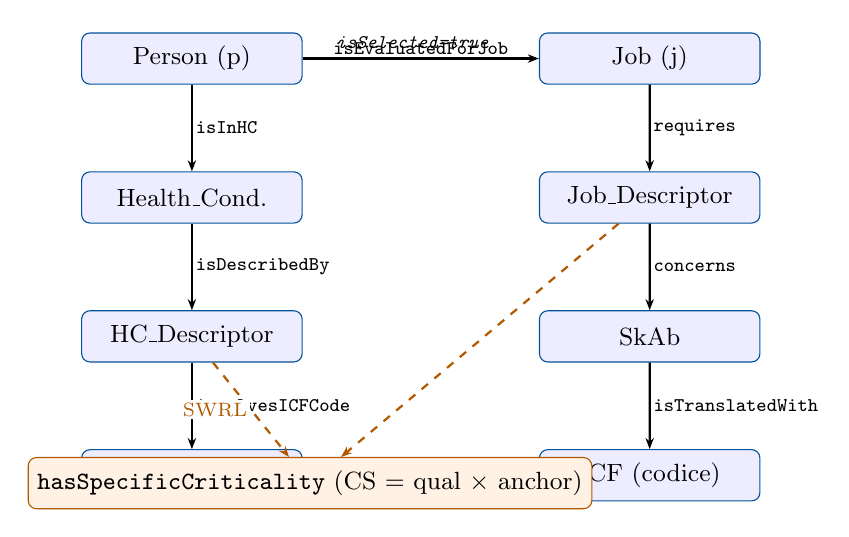
\begin{tikzpicture}[scale=0.85,
  lbl/.style={font=\scriptsize, fill=white, inner sep=1pt},
  node distance=1.1cm and 2cm,
  ent/.style={rectangle, draw=rientraBlue, fill=blue!7, rounded corners=3pt,
              minimum width=2.8cm, minimum height=0.65cm, align=center, font=\small},
  inf/.style={rectangle, draw=orange!70!black, fill=orange!10, rounded corners=3pt,
              minimum width=2.8cm, minimum height=0.65cm, align=center, font=\small},
  prop/.style={font=\scriptsize\itshape, above},
  propb/.style={font=\scriptsize\itshape, below},
  arrow/.style={-{Stealth[length=4pt]}, thick},
  darrow/.style={-{Stealth[length=4pt]}, thick, dashed, orange!70!black},
]
  % Left column: Person side
  \node[ent] (person) {Person (p)};
  \node[ent, below=of person] (hc) {Health\_Cond.};
  \node[ent, below=of hc] (des) {HC\_Descriptor};
  \node[ent, below=of des] (icf) {ICF (codice)};

  \draw[arrow] (person) -- node[lbl, right] {\texttt{isInHC}} (hc);
  \draw[arrow] (hc) -- node[lbl, right] {\texttt{isDescribedBy}} (des);
  \draw[arrow] (des) -- node[lbl, right] {\texttt{involvesICFCode}} (icf);

  % Right column: Job side
  \node[ent, right=3.0cm of person] (job) {Job (j)};
  \node[ent, below=of job] (jde) {Job\_Descriptor};
  \node[ent, below=of jde] (skab) {SkAb};
  \node[ent, below=of skab] (icf2) {ICF (codice)};

  \draw[arrow] (job) -- node[lbl, right] {\texttt{requires}} (jde);
  \draw[arrow] (jde) -- node[lbl, right] {\texttt{concerns}} (skab);
  \draw[arrow] (skab) -- node[lbl, right] {\texttt{isTranslatedWith}} (icf2);

  % Join arrow
  \draw[arrow, <->, thick, red!60!black] (icf) --
    node[midway, below, font=\scriptsize\bfseries, red!60!black, fill=white, inner sep=1pt]
    {join ICF} (icf2);

  % Pellet inference
  \node[inf, below=1.2cm of des, xshift=1.5cm] (cs)
    {\texttt{hasSpecificCriticality} (CS = qual $\times$ anchor)};
  \draw[darrow] (des) -- node[lbl, left] {SWRL} (cs);
  \draw[darrow] (jde) -- (cs);

  % Top connection
  \draw[arrow] (person) -- node[lbl, above] {\texttt{isEvaluatedForJob}} (job);
  \node[font=\scriptsize\itshape, right=0.3cm of person, yshift=0.2cm]
    {\texttt{isSelected=true}};
\end{tikzpicture}%
}% end resizebox
\caption{Struttura del grafo di matching: il join sul codice ICF collega
la condizione di salute del lavoratore alle skill richieste dal job.}
\end{figure}

% ============================================================
\section{Setup, deployment e configurazione}
% ============================================================

\subsection{Requisiti di sistema}

\begin{table}[H]
\centering
\caption{Requisiti software del microservizio.}
\begin{tabular}{L{4cm} L{3.5cm} L{5cm}}
\toprule
\textbf{Componente} & \textbf{Versione minima} & \textbf{Note} \\
\midrule
Python & 3.11+ & Necessario per \texttt{match-case}, type hints avanzati \\
Java & 11+ & Richiesto da Pellet via owlready2; deve essere nel \texttt{PATH} \\
Sistema operativo & Linux / macOS / Windows & Test primari su Linux \\
\bottomrule
\end{tabular}
\end{table}

\begin{warningbox}[Java obbligatorio nel PATH]
owlready2 avvia Pellet come sottoprocesso JVM. Se \texttt{java} non \`{e}
disponibile nel \texttt{PATH} del processo Python, il caricamento
dell'ontologia fallisce con un errore poco descrittivo. Verificare
sempre con \texttt{java -version} (deve restituire versione $\geq$ 11)
prima di avviare il servizio.
\end{warningbox}

\subsection{Dipendenze Python (\texttt{requirements.txt})}

\begin{table}[H]
\centering
\caption{Dipendenze Python con versioni minime e motivazioni.}
\begin{tabular}{L{4.5cm} L{2.5cm} L{5.5cm}}
\toprule
\textbf{Pacchetto} & \textbf{Versione} & \textbf{Motivazione} \\
\midrule
\texttt{fastapi} & $\geq$ 0.111.0 &
  Framework ASGI; 0.111 introduce il \texttt{lifespan} stabile e
  Pydantic v2 come default. \\[3pt]
\texttt{uvicorn[standard]} & $\geq$ 0.29.0 &
  Server ASGI; \texttt{[standard]} include \texttt{httptools} e
  \texttt{uvloop} per prestazioni ottimali su Linux. \\[3pt]
\texttt{pydantic} & $\geq$ 2.0.0 &
  Validazione e serializzazione; v2 richiesta dai modelli
  di \texttt{models.py}. \\[3pt]
\texttt{owlready2} & $\geq$ 0.46 &
  Interfaccia Python a OWL/Pellet; 0.46 risolve bug
  critici nella gestione di SWRL built-in. \\[3pt]
\texttt{morph-kgc} & $\geq$ 2.6.0 &
  Materializzatore R2RML W3C per la pipeline di import SQL. \\[3pt]
\texttt{rdflib} & $\geq$ 6.3.2 &
  Lettura/scrittura di grafi RDF; usato da \texttt{importer.py}
  e da \texttt{inject\_imported\_workers()}. \\[3pt]
\texttt{python-multipart} & $\geq$ 0.0.9 &
  Richiesto da FastAPI per \texttt{UploadFile} / \texttt{File(...)}. \\[3pt]
\texttt{sqlalchemy} & $\geq$ 2.0.0 &
  Richiesto da morph-kgc per le connessioni ai DB relazionali. \\
\bottomrule
\end{tabular}
\end{table}

\begin{infobox}[owlready2 e rdflib: coesistenza]
owlready2 usa internamente rdflib per il parsing RDF, ma la versione
interna pu\`{o} differire da quella installata esplicitamente.
L'installazione esplicita di \texttt{rdflib>=6.3.2} garantisce che il
codice di \texttt{inject\_imported\_workers()} usi la versione corretta
dell'API (\texttt{Graph.parse()}, \texttt{Graph.objects()}) senza
conflitti.
\end{infobox}

\subsection{Procedure di installazione}

Il virtual environment \`{e} \textbf{fortemente raccomandato} per due ragioni
specifiche al progetto: owlready2 installa binari nativi (JNI bridge) che
possono entrare in conflitto con altre versioni installate a livello di sistema;
morph-kgc ha dipendenze (SQLAlchemy, rdflib) con versioni minime precise che
potrebbero non coincidere con quelle del sistema. Il venv isola il progetto
e garantisce riproducibilit\`{a} tra ambienti diversi.

\begin{lstlisting}[language=bash, caption={Setup completo dell'ambiente di sviluppo.}]
# 1. Creare e attivare il virtual environment
python3 -m venv .venv
source .venv/bin/activate        # Linux/macOS
# .venv\Scripts\activate         # Windows

# 2. Installare le dipendenze
pip install -r requirements.txt

# 3. Verificare Java
java -version   # deve essere >= 11

# 4a. Avvio con auto-detection del file RDF
#     (posizionare il .rdf nella directory del servizio)
uvicorn main:app --host 0.0.0.0 --port 8000

# 4b. Avvio con percorso esplicito
ONTOLOGY_PATH=/path/to/ontology.rdf \
  uvicorn main:app --host 0.0.0.0 --port 8000

# 5. Polling della readiness (Pellet impiega 30-120 s)
curl http://localhost:8000/status
# Attendere {"status": "ready", ...}
\end{lstlisting}

\noindent \subsection{Modalit\`{a} di avvio e readiness}

Il servizio implementa un \textbf{warm-up asincrono}: risponde
immediatamente (HTTP 200) alla rotta \texttt{/status} con
\texttt{\{"status": "loading"\}} sin dal primo istante, mentre Pellet
lavora in background. Il codice 503 (\textit{Service Unavailable}) \`{e}
stato scelto rispetto ad alternative come 425 (\textit{Too Early}) o 202
(\textit{Accepted}) perch\'{e}: 503 \`{e} universalmente supportato dai
client HTTP e segnala inequivocabilmente che il servizio esiste ma non
\`{e} ancora operativo, incoraggiando il retry; 425 non \`{e} supportato
da tutte le versioni di Spring Boot e dai client HTTP generici; 202 implica
che la richiesta \`{e} stata accettata e sar\`{a} processata in asincrono,
semantica non corretta per un endpoint di lettura sincrono.

Il \textbf{polling HTTP} \`{e} preferito a WebSocket o Server-Sent Events
perch\'{e}: (1) il warm-up \`{e} un evento una-tantum, non un flusso
continuo; (2) il polling su \texttt{/status} non richiede gestione della
connessione persistente n\'{e} autenticazione aggiuntiva; (3) in contesto
Electron/localhost la latenza del polling \`{e} trascurabile ($<$1ms).
Tutte le altre rotte restituiscono \texttt{HTTP 503}
fino a completamento. Il frontend deve implementare un ciclo di polling
su \texttt{GET /status} e sbloccare la UI solo quando
\texttt{status == "ready"}.

\begin{table}[H]
\centering
\caption{Comportamento degli endpoint durante il warm-up.}
\begin{tabular}{L{4cm} C{3cm} L{5.5cm}}
\toprule
\textbf{Condizione} & \textbf{HTTP} & \textbf{Note} \\
\midrule
Pellet in esecuzione & 200 (solo \texttt{/status}) & Risponde \texttt{status: "loading"} \\
Pellet in esecuzione & 503 (tutti gli altri) & Cache snapshot disponibile se gi\`{a} esistente \\
Pellet completato & 200 & Tutti gli endpoint operativi \\
Errore Pellet & 500 & \texttt{GET /status} descrive l'errore \\
\bottomrule
\end{tabular}
\end{table}

\subsection{Integrazione con Spring Boot}

Il servizio \`{e} progettato per essere chiamato da uno Spring Boot
Backend sulla porta 8080. L'integrazione tipica usa \texttt{RestTemplate}
o \texttt{WebClient}:

\begin{lstlisting}[language=Java, caption={Esempio di chiamata da Spring Boot con RestTemplate.}]
@Service
public class SemanticService {

    private final RestTemplate restTemplate;
    private final String baseUrl = "http://localhost:8000";

    public String getWorkers() {
        return restTemplate.getForObject(
            baseUrl + "/workers", String.class);
    }

    public String getMatchResults(String workerId) {
        return restTemplate.getForObject(
            baseUrl + "/match/" + workerId, String.class);
    }
}
\end{lstlisting}

\noindent Il CORS \`{e} pre-configurato per accettare richieste da
\texttt{http://localhost:8080} (Spring Boot), \texttt{http://localhost:5173}
(React/Vite) e \texttt{http://localhost:3000} (React alternativo).
Non \`{e} implementata autenticazione a livello del microservizio:
la gestione auth \`{e} delegata interamente a Spring Boot.

\subsection{Configurazione Pyright (\texttt{pyrightconfig.json})}

\begin{lstlisting}[caption={\texttt{pyrightconfig.json} --- configurazione del type checker.}]
{
  "venvPath": ".",
  "venv": ".venv",
  "pythonVersion": "3.14",
  "typeCheckingMode": "off"
}
\end{lstlisting}

\noindent \begin{table}[H]
\centering
\caption{Motivazione di ogni campo \texttt{pyrightconfig.json}.}
\begin{tabular}{L{4cm} L{8.5cm}}
\toprule
\textbf{Campo} & \textbf{Motivazione} \\
\midrule
\texttt{venvPath: "."} &
  Pyright cerca il virtual environment nella directory corrente del progetto. \\[3pt]
\texttt{venv: ".venv"} &
  Nome standard del virtual environment generato da \texttt{python -m venv .venv}. \\[3pt]
\texttt{pythonVersion: "3.14"} &
  Impostato alla versione futura per evitare falsi positivi su sintassi
  moderna (type union \texttt{X | Y}, \texttt{match-case}) gi\`{a} usata
  nel codice ma non ancora pienamente supportata da Pyright per versioni
  precedenti. Il valore non influenza il runtime, solo l'analisi statica. \\[3pt]
\texttt{typeCheckingMode: "off"} &
  La type-checking \`{e} disabilitata perch\'{e} owlready2 non ha stub
  di tipo (\texttt{.pyi}) completi. Pyright genererebbe centinaia di
  errori su attributi dinamici degli oggetti owlready2, oscurando
  problemi reali. La configurazione attuale permette l'uso di Pyright
  per il completamento automatico e la navigazione del codice senza
  il rumore dei type errors. \\
\bottomrule
\end{tabular}
\end{table}

\begin{warningbox}[pythonVersion: "3.14" vs runtime]
Il valore \texttt{3.14} in \texttt{pyrightconfig.json} \`{e} la versione
\textit{di analisi} di Pyright, non la versione di runtime. Il codice
richiede Python \textbf{3.11+} in esecuzione (come specificato in
\texttt{requirements.txt} e \texttt{README.md}). Impostare
\texttt{3.11} o \texttt{3.12} in pyrightconfig non cambierebbe il
comportamento runtime ma potrebbe causare warning su sintassi che
Pyright considera ancora sperimentale.
\end{warningbox}

% ============================================================
\section{Modulo \texttt{import\_workers/importer.py} --- Pipeline RDB2RDF}
% ============================================================

\subsection{Ruolo, contesto e versione}

\texttt{importer.py} implementa la \textbf{pipeline RDB2RDF} del progetto
Rientr@: converte dataset di pazienti in formato SQL in individui OWL
compatibili con Pellet, iniettandoli nell'ontologia \texttt{Rientra.rdf}
senza alterarne la struttura originale.

Il modulo \`{e} la \textit{versione libreria} di \texttt{rientra\_import.py}
(strumento CLI della cartella Union), adattata per essere chiamata
programmaticamente dagli endpoint FastAPI (\texttt{POST /import/workers})
invece che da riga di comando. La versione documentata corrisponde al
\textbf{prototipo strategico v0.1-test} (aprile 2026), sviluppato per
validare la strategia implementativa RDB2RDF. Le funzionalit\`{a} legate
all'interfaccia grafica (selezione interattiva dei job, avvio matching,
validazione in tempo reale) non sono incluse in questa versione.

Il modulo appartiene al package \texttt{import\_workers/}, segnalato dal
file \texttt{\_\_init\_\_.py} (contenuto: sola riga di commento identificativa).
Questa struttura a package permette di importare il modulo con
\texttt{from import\_\allowbreak{}workers.importer import ...} da \texttt{main.py}.

\subsection{Perch\'{e} RDB2RDF: motivazione del paradigma}

\begin{infobox}[Scelta paradigmatica --- RDB2RDF vs manipolazione testuale]
RDB2RDF garantisce \textbf{interoperabilit\`{a}}, \textbf{riproducibilit\`{a}}
e \textbf{manutenibilit\`{a}} del processo di import, in linea con gli
standard del Web Semantico W3C. Un approccio ad-hoc basato su
manipolazione testuale del file RDF non sarebbe documentabile,
verificabile n\'{e} riusabile con altri strumenti ontologici.
\end{infobox}

Il W3C definisce due approcci RDB2RDF:

\begin{table}[H]
\centering\small
\caption{Confronto Direct Mapping vs R2RML per il caso Rientr@.}
\begin{tabular}{L{3.8cm} L{3.5cm} L{5cm}}
\toprule
\textbf{Aspetto} & \textbf{Direct Mapping} & \textbf{R2RML (adottato)} \\
\midrule
Struttura IRI & Generata dai nomi colonne & Template espliciti (Section~\ref{sec:iri}) \\
Costanti & Non supportate & \texttt{rr:constant} \\
Logica condizionale & Non supportata & VIEW SQL ausiliarie \\
Filtraggio & Non supportato & JOIN su tabelle di controllo \\
Datatype & Inferiti & Dichiarati esplicitamente \\
Auditabilit\`{a} & Nessuna & File \texttt{.ttl} versionabile in Git \\
\bottomrule
\end{tabular}
\end{table}

Il Direct Mapping \`{e} inapplicabile per quattro ragioni specifiche al
dominio Rientr@:
\begin{enumerate}
  \item Gli IRI devono rispettare la struttura
        \texttt{Person-CommonBox\#\{person\_\allowbreak{}id\}} / \texttt{RientraHC\#des\_\{id\}\_\{icf\}}
        non derivabile automaticamente dai nomi delle colonne SQL.
  \item La propriet\`{a} \texttt{isSelected} deve essere sempre \texttt{false}
        come costante applicativa (non da colonna).
  \item I qualifier ICF (\texttt{BFqual}/\texttt{AP1qual}/\texttt{BS1qual})
        dipendono dal prefisso del codice (b/d/s): logica condizionale non
        esprimibile in Direct Mapping.
  \item I codici \texttt{e*} e i job non presenti nell'ontologia devono
        essere esclusi automaticamente.
\end{enumerate}

\subsection{Perch\'{e} Morph-KGC come engine R2RML}

\begin{infobox}[Scelta engine --- Morph-KGC vs RMLMapper vs D2RQ]
Morph-KGC \`{e} stato scelto per la sua \textbf{integrazione nativa con
Python}, il supporto a SQLite via SQLAlchemy, e la restituzione diretta
di un grafo rdflib senza file intermedi su disco.
\end{infobox}

\begin{table}[H]
\centering\small
\caption{Confronto engine R2RML.}
\begin{tabular}{L{3.5cm} L{3cm} L{6cm}}
\toprule
\textbf{Engine} & \textbf{Linguaggio} & \textbf{Motivo esclusione / adozione} \\
\midrule
RMLMapper & Java & Richiede JVM + invocazione \texttt{subprocess}; integrazione
             complessa in pipeline Python. \\
D2RQ & Java & Non pi\`{u} mantenuto attivamente; supporto DB limitato. \\
\textbf{Morph-KGC} & \textbf{Python} & \textbf{Adottato}: API Python nativa;
             \texttt{materialize(config)} restituisce \texttt{rdflib.Graph}
             in memoria; supporto SQLite; conformit\`{a} R2RML W3C; sviluppo
             attivo (UPM Madrid). \\
\bottomrule
\end{tabular}
\end{table}

\begin{warningbox}[Limitazione nota su macOS]
Su macOS, Morph-KGC non supporta la parallelizzazione quando invocato
come libreria Python. Il messaggio \textit{``Parallelization is not
supported for darwin when running as a library''} \`{e} atteso e non
influisce sulla correttezza dei risultati.
\end{warningbox}

\subsection{Dipendenze e importazione condizionale}

\subsubsection{Pattern \texttt{\_DEPS\_OK} e stub \texttt{\_SAFE\_ANY}}

\begin{lstlisting}[caption={Importazione condizionale con fallback graceful.}]
_SAFE_ANY: Any = None

try:
    import morph_kgc
    from rdflib import Graph, URIRef, Namespace
    from rdflib.namespace import RDF, OWL, RDFS, XSD
    _DEPS_OK = True
except ImportError:
    _DEPS_OK = False
    morph_kgc: Any = _SAFE_ANY  # type: ignore[no-redef]
    Graph:     Any = _SAFE_ANY  # ...
    # ... altri stub
    logger.warning("morph_kgc or rdflib not installed...")
\end{lstlisting}

\noindent Le dipendenze heavy (\texttt{morph\_kgc}, \texttt{rdflib}) sono importate
in un blocco \texttt{try/except ImportError}. Se assenti, il modulo si
carica comunque con \texttt{\_DEPS\_OK = False}: ogni funzione che le
richiede fallisce con un \texttt{RuntimeError} descrittivo anzich\'{e}
con un \texttt{ImportError} al momento del caricamento del modulo.

Il tipo \texttt{\_SAFE\_ANY} (alias di \texttt{Any}) viene assegnato
agli stub per i nomi non importati. Pyrefly/Pyright tratta \texttt{Any}
come compatibile con ogni operazione (chiamata, accesso attributo,
subscript), evitando che gli errori di tipo dagli stub si propaghino
al resto del codice analizzato staticamente.

Questo pattern garantisce che il microservizio FastAPI si avvii
correttamente anche in ambienti dove morph-kgc non \`{e} installato,
degradando gracefully solo la funzionalit\`{a} di import.

\subsubsection{Namespace e costanti di modulo}
\vspace{2pt}
\begin{lstlisting}[caption={Namespace rdflib e costanti di modulo.}]
if _DEPS_OK:
    NS_FOAF    = Namespace("http://www.stiima.cnr.it/FOAF-excerpt#")
    NS_HC      = Namespace("http://www.stiima.cnr.it/RientraHC#")
    NS_ICF     = Namespace("http://www.stiima.cnr.it/ICF-exc-coreset#")
    NS_PERSON  = Namespace("http://www.stiima.cnr.it/Person-CommonBox#")
    NS_JOB     = Namespace("http://www.stiima.cnr.it/JobList#")
    NS_RIEONT3 = Namespace("http://www.stiima.cnr.it/RientraOnt3#")
else:
    NS_FOAF = NS_HC = ... = _SAFE_ANY

CLOSING_TAG   = "</rdf:RDF>"   # marcatore per l'iniezione testuale
QUALIFIER_MAP = {"b": "BFqual", "d": "AP1qual", "s": "BS1qual"}
\end{lstlisting}

\noindent I namespace rispecchiano esattamente quelli dichiarati nel file RDF
(Sezione~10). \texttt{QUALIFIER\_MAP} codifica il routing
b/d/s $\rightarrow$ propriet\`{a} ICF, coerente con
\texttt{\_is\_ap1\_code()} in \texttt{reasoner.py}.
\texttt{CLOSING\_TAG} \`{e} il punto di iniezione testuale nell'ontologia.

\subsubsection{\texttt{ImportResult} --- dataclass di risposta}

\begin{lstlisting}[caption={\texttt{ImportResult} --- struttura dati di ritorno.}]
@dataclass
class ImportResult:
    persons_added:   int = 0
    persons_skipped: int = 0
    icf_valid:       int = 0
    icf_skipped:     int = 0
    jobs_valid:      int = 0
    jobs_skipped:    int = 0
    backup_path:     str = ""
    new_person_ids:  list[str] = field(default_factory=list)
    skipped_ids:     list[str] = field(default_factory=list)
    error:           Optional[str] = None
\end{lstlisting}

\noindent L'uso di \texttt{@dataclass} anzich\'{e} un Pydantic \texttt{BaseModel}
\`{e} intenzionale: \texttt{ImportResult} \`{e} un oggetto di trasferimento
interno tra \texttt{importer.py} e \texttt{main.py}, non un modello di
validazione REST. \texttt{main.py} lo converte manualmente in un
\texttt{JSONResponse} prima di restituirlo al client. Il campo
\texttt{error = None} indica successo; se valorizzato contiene il
messaggio dell'eccezione catturata.

\subsection{Funzione pubblica \texttt{ensure\_mapping()}}

\begin{lstlisting}[caption={\texttt{ensure\_mapping()} --- generazione idempotente del mapping.}]
def ensure_mapping(ontology_path: str, mapping_path: str) -> None:
    if not _DEPS_OK:
        raise RuntimeError("morph-kgc / rdflib non installati.")
    mapping = Path(mapping_path)
    if mapping.exists():
        logger.info("[importer] Mapping file already exists: %s", mapping)
        return     # no-op: gia' presente
    logger.info("[importer] Generating mapping from ontology...")
    _generate_mapping(ontology_path, mapping_path)
\end{lstlisting}

\noindent Questa funzione \`{e} chiamata dal \textit{lifespan handler} di
\texttt{main.py} a ogni avvio. L'idempotenza (no-op se il file esiste gi\`{a}) \`{e} fondamentale
perch\'{e} il \textit{lifespan handler} viene eseguito ad ogni avvio
del servizio: senza il controllo di esistenza, il mapping verrebbe
rigenerato ad ogni riavvio, causando un parsing completo dell'ontologia
($\sim$12.000 triple, diversi secondi) anche quando non \`{e} cambiato
nulla. Il design idempotente rispetta anche il principio di \textit{least
surprise}: chiamare \texttt{ensure\_mapping} due volte ha lo stesso
effetto di chiamarla una sola volta.
Il mapping va rigenerato \textit{solo} in caso di modifiche strutturali
all'ontologia (nuove propriet\`{a} datatype, nuovi namespace, nuove classi),
non per ogni import di nuovi pazienti.

\subsection{Generazione del mapping R2RML --- \texttt{\_generate\_mapping()}}

Questa \`{e} la funzione architetturalmente pi\`{u} importante del modulo:
analizza l'ontologia OWL e produce un file \texttt{rientra\_mapping.ttl}
\textit{derivato automaticamente} dalla struttura delle propriet\`{a} OWL.

\subsubsection{Scoperta automatica delle propriet\`{a} FOAF:Person}

\begin{lstlisting}[caption={Classificazione automatica delle datatype properties.}]
for prop in g.subjects(RDF.type, OWL.DatatypeProperty):
    domain = next(g.objects(prop, RDFS.domain), None)
    range_ = next(g.objects(prop, RDFS.range),  None)
    if str(domain) != str(foaf_person):
        continue           # solo prop. di FOAF:Person
    prop_name = str(prop).split("#")[-1]
    range_str = str(range_) if range_ else str(XSD.string)
    if range_str == str(XSD.boolean):
        boolean_props[prop_name] = prop    # isSelected, selectedJob
    elif range_str in XSD_PLAIN or range_ is None:
        plain_props[prop_name]   = prop    # first_name, surname, TIN, ...
    else:
        typed_props[prop_name]   = (xsd_type, prop)  # birthday, ZIPcode
\end{lstlisting}

\noindent Le propriet\`{a} vengono partizionate in tre gruppi:
\begin{itemize}[noitemsep]
  \item \texttt{plain\_props}: stringhe senza datatype esplicito
        (serializzate come plain literal in R2RML).
  \item \texttt{typed\_props}: valori con datatype XSD non stringa
        (\texttt{xsd:dateTime}, \texttt{xsd:int}) --- serializzati con
        \texttt{rr:datatype}.
  \item \texttt{boolean\_props}: propriet\`{a} booleane --- gestite con
        \texttt{rr:constant} ma \textbf{escluse dalla serializzazione XML}
        per il problema Pellet (Section~\ref{sec:boolean}).
\end{itemize}

L'approccio di scoperta automatica garantisce che il mapping sia sempre
aggiornato alla struttura OWL corrente senza modifiche manuali al codice.

Analogamente, le propriet\`{a} di \texttt{HC\_Descriptor} (\texttt{BFqual},
\texttt{AP1qual}, \texttt{BS1qual}) vengono scoperte filtrando per dominio
\texttt{hc:HC\_Descriptor}.

\subsubsection{Correzione colonna \texttt{ZIPcode}}

\begin{lstlisting}[caption={Alias colonna ZIPcode $\rightarrow$ zip\_code.}]
col = "zip_code" if prop_name == "ZIPcode" else prop_name
\end{lstlisting}

\noindent La propriet\`{a} OWL si chiama \texttt{ZIPcode} (naming OWL), ma la
colonna SQL nella tabella \texttt{person} si chiama \texttt{zip\_code}
(snake\_case SQL). Questo mapping esplicito risolve la discrepanza di
naming senza modificare n\'{e} l'ontologia n\'{e} lo schema SQL.

\subsubsection{Le 5 TriplesMap del mapping R2RML}

Il mapping generato contiene esattamente \textbf{5 TriplesMap},
ciascuna con una responsabilit\`{a} precisa:

\begin{table}[H]
\centering\small
\caption{Le 5 TriplesMap di \texttt{rientra\_mapping.ttl}.}
\begin{tabular}{L{3.5cm} L{3.5cm} L{5.5cm}}
\toprule
\textbf{TriplesMap} & \textbf{Sorgente} & \textbf{Triple prodotte} \\
\midrule
\texttt{\#PersonMap} &
  \texttt{person} &
  Individuo \texttt{foaf:Person} con tutte le datatype prop. anagrafiche.
  IRI: \texttt{Person-CommonBox\#\{person\_\allowbreak{}id\}} \\[4pt]
\texttt{\#HealthCond.\-Map} &
  \texttt{person} &
  Individuo \texttt{hc:Health\_Condition}.
  IRI: \texttt{Person-CommonBox\#HC\{person\_\allowbreak{}id\}} \\[4pt]
\texttt{\#DescriptorMapB} &
  \texttt{v\_desc\_b} &
  Individui \texttt{HC\_Descriptor} per codici b*.
  Propriet\`{a} \texttt{BFqual}. \\[4pt]
\texttt{\#DescriptorMapD} &
  \texttt{v\_desc\_d} &
  Individui \texttt{HC\_Descriptor} per codici d*.
  Propriet\`{a} \texttt{AP1qual}. \\[4pt]
\texttt{\#DescriptorMapS} &
  \texttt{v\_desc\_s} &
  Individui \texttt{HC\_Descriptor} per codici s*.
  Propriet\`{a} \texttt{BS1qual}. \\[4pt]
\texttt{\#DescriptorLinkMap} &
  \texttt{v\_hc\_links} &
  Triple \texttt{HC isDescribedBy Descriptor} (una per codice ICF). \\[4pt]
\texttt{\#JobEvaluationMap} &
  \texttt{v\_job\_valid} &
  Triple \texttt{Person isEvaluatedForJob Job}
  (solo job presenti nell'ontologia). \\
\bottomrule
\end{tabular}
\end{table}

\subsubsection{Il mapping generato: \texttt{rientra\_mapping.ttl}}

Il file prodotto da \texttt{\_generate\_mapping()} \`{e} un artefatto
documentale autonomo: versionabile in Git, revisionabile da un ontology
engineer, e conforme allo standard W3C R2RML. Un estratto del file
effettivo generato per l'ontologia Rientr@ v3.1:

\begin{lstlisting}[caption={Estratto da \texttt{rientra\_mapping.ttl} --- MAP 1 e MAP 3B.}, numbers=none]
<#PersonMap>
    rr:logicalTable [ rr:tableName "person" ] ;
    rr:subjectMap [
        rr:template ".../Person-CommonBox#{person_id}" ;
        rr:class foaf:Person ; rr:class owl:NamedIndividual
    ] ;
    rr:predicateObjectMap [
        rr:predicate <.../FOAF-excerpt#first_name> ;
        rr:objectMap [ rr:column "first_name" ]
    ] ;
    ...
    rr:predicateObjectMap [
        rr:predicate <.../RientraOnt3Merged#isSelected> ;
        rr:objectMap [ rr:constant "false"^^xsd:boolean ]
    ] .

<#DescriptorMapB>
    rr:logicalTable [ rr:tableName "v_desc_b" ] ;
    rr:subjectMap [
        rr:template ".../RientraHC#des_{person_id}_{icf_code}" ;
        rr:class hc:HC_Descriptor ; rr:class owl:NamedIndividual
    ] ;
    rr:predicateObjectMap [
        rr:predicate hc:involvesICFCode ;
        rr:objectMap [
            rr:template ".../ICF-exc-coreset#{icf_code}" ;
            rr:termType rr:IRI
        ]
    ] ;
    rr:predicateObjectMap [
        rr:predicate hc:BFqual ;
        rr:objectMap [ rr:column "qualifier" ; rr:datatype xsd:integer ]
    ] .
\end{lstlisting}

\noindent \begin{warningbox}[Nota sul file reale: datatype hash in luogo di xsd:integer]
Nel file \texttt{rientra\_mapping.ttl} generato, le TriplesMap B, D, S
mostrano un datatype con hash (es.\
\texttt{xsd:N1333c4ff5bdc4100a43de2255a2eda34}) anzich\'{e}
\texttt{xsd:integer}. Questo \`{e} un artefatto di come rdflib serializza
i blank node del range della propriet\`{a} quando il tipo XSD non \`{e}
riconosciuto come tipo primitivo noto. Il comportamento runtime di
Morph-KGC \`{e} corretto perch\'{e} il valore viene passato comunque come
intero dalla colonna SQL. Questo \`{e} un punto di miglioramento futuro:
sostituire il lookup dinamico del range con un mapping fisso
\texttt{\{''BFqual'': ''integer'', ...\}}.
\end{warningbox}

\subsection{Perch\'{e} le VIEW SQL invece di query R2RML complesse}
\label{sec:views}

\begin{infobox}[Scelta architetturale --- VIEW SQL]
Le VIEW SQL esprimono logiche di filtraggio e routing che R2RML standard
non supporta nativamente (logica condizionale sui prefissi ICF, join su
liste di valori validi), mantenendo il mapping Turtle semplice e leggibile.
\end{infobox}

\subsubsection{\texttt{\_\allowbreak{}create\_\allowbreak{}views(conn, known\_\allowbreak{}icf, known\_\allowbreak{}jobs)}}

\begin{lstlisting}[caption={Creazione delle VIEW ausiliarie nel DB SQLite in-memory.}]
# Tabelle di controllo (popolate dinamicamente dall'ontologia)
conn.execute("CREATE TABLE _known_icf  (icf_code TEXT PRIMARY KEY)")
conn.execute("CREATE TABLE _known_jobs (job_id   TEXT PRIMARY KEY)")
conn.executemany("INSERT OR IGNORE INTO _known_icf  VALUES (?)", ...)
conn.executemany("INSERT OR IGNORE INTO _known_jobs VALUES (?)", ...)

# VIEW per routing prefisso ICF
for view, prefix in [("v_desc_b", "b"), ("v_desc_d", "d"), ("v_desc_s", "s")]:
    conn.execute(f"""
        CREATE VIEW {view} AS
        SELECT h.person_id, h.icf_code, h.qualifier
        FROM hc_descriptor h
        JOIN _known_icf k ON k.icf_code = h.icf_code
        WHERE lower(substr(h.icf_code,1,1)) = '{prefix}'
    """)

# VIEW unione per isDescribedBy
conn.execute("""
    CREATE VIEW v_hc_links AS
    SELECT person_id, icf_code FROM v_desc_b
    UNION ALL SELECT ... FROM v_desc_d
    UNION ALL ... FROM v_desc_s
""")

# VIEW per job validi (con try/except: tabella job_evaluation opzionale)
conn.execute("""
    CREATE VIEW v_job_valid AS
    SELECT j.person_id, j.job_id
    FROM job_evaluation j
    JOIN _known_jobs k ON k.job_id = j.job_id
""")
\end{lstlisting}

\noindent \begin{table}[H]
\centering\small
\caption{VIEW SQL ausiliarie e loro scopo.}
\begin{tabular}{L{3cm} L{3.5cm} L{6cm}}
\toprule
\textbf{VIEW} & \textbf{Filtro} & \textbf{Scopo} \\
\midrule
\texttt{v\_desc\_b} & codici ICF \texttt{b*} noti & Alimenta MAP 3B $\rightarrow$ \texttt{BFqual} \\
\texttt{v\_desc\_d} & codici ICF \texttt{d*} noti & Alimenta MAP 3D $\rightarrow$ \texttt{AP1qual} \\
\texttt{v\_desc\_s} & codici ICF \texttt{s*} noti & Alimenta MAP 3S $\rightarrow$ \texttt{BS1qual} \\
\texttt{v\_hc\_links} & unione b+d+s & Alimenta MAP 4 $\rightarrow$ \texttt{isDescribedBy} \\
\texttt{v\_job\_valid} & job presenti nell'ontologia & Alimenta MAP 5 $\rightarrow$ \texttt{isEvaluatedForJob} \\
\bottomrule
\end{tabular}
\end{table}

Le tabelle \texttt{\_known\_icf} e \texttt{\_known\_jobs} vengono
\textbf{popolate dinamicamente} dall'ontologia prima di ogni esecuzione
(tramite \texttt{\_extract\_known\_icf()} e \texttt{\_extract\_known\_jobs()}).
Questo garantisce che il filtraggio sia sempre aggiornato anche se
l'ontologia viene estesa con nuovi codici ICF o nuovi job, senza modificare
n\'{e} il codice n\'{e} il mapping.

I codici \texttt{e*} (Environmental Factors) vengono automaticamente
esclusi perch\'{e} nessuna VIEW li include: non esistono n\'{e}
\texttt{v\_desc\_e} n\'{e} un match in \texttt{\_known\_icf} per
codici con prefisso \texttt{e}.

La gestione della tabella \texttt{job\_evaluation} (opzionale nel dataset)
avviene tramite \texttt{try/except sqlite3.Error}: se la tabella non
esiste, viene creata una VIEW vuota, il che porta a zero link
\texttt{isEvaluatedForJob} senza errori.

\subsection{Perch\'{e} SQLite in-memory}

\begin{infobox}[Scelta database --- SQLite in-memory]
SQLite in-memory garantisce \textbf{zero configurazione}, \textbf{isolamento
completo} tra esecuzioni e \textbf{riproducibilit\`{a} totale}: ogni run
parte da uno stato pulito, senza residui di esecuzioni precedenti.
\end{infobox}

\subsubsection{\texttt{\_load\_sql(sql\_path)}}

\begin{lstlisting}[caption={Caricamento del dataset SQL in SQLite in-memory.}]
def _load_sql(sql_path: str) -> sqlite3.Connection:
    sql  = Path(sql_path).read_text(encoding="utf-8")
    conn = sqlite3.connect(":memory:")
    conn.row_factory = sqlite3.Row  # accesso per nome colonna
    conn.executescript(sql)
    return conn
\end{lstlisting}

\noindent \texttt{sqlite3.connect(":memory:")} crea un database completamente in RAM.
\texttt{conn.row\_\allowbreak{}factory = sqlite3.Row} abilita l'accesso ai risultati
per nome di colonna (\texttt{row["person\_id"]}) anzich\'{e} per indice,
migliorando la leggibilit\`{a} e la robustezza del codice.
\texttt{executescript()} esegue il file SQL completo in una singola
transazione.

Il vincolo che Morph-KGC richiede un file su disco per la connessione
SQLAlchemy viene risolto da \texttt{\_export\_db\_to\_file()}, che usa
\texttt{conn.iterdump()} per scrivere il DB in-memory su un file
temporaneo, che viene poi eliminato in un blocco \texttt{finally}.

\subsection{Struttura del dataset SQL di input}

Il file SQL importato deve definire le seguenti tabelle. La struttura
a tre tabelle separate (\texttt{person}, \texttt{hc\_descriptor},
\texttt{job\_evaluation}) anzich\'{e} una tabella piatta riflette la
struttura dell'ontologia: Person, HC e Descriptor sono entit\`{a}
distinte con IRI propri e relazioni molti-a-molti (una persona ha
molti codici ICF; un codice ICF pu\`{o} appartenere a molte persone).
Una tabella piatta con colonne \texttt{person\_\allowbreak{}id, icf\_\allowbreak{}code, qualifier, job\_\allowbreak{}id}
avrebbe righe duplicate per ogni persona con pi\`{u} codici e pi\`{u} job,
complicando il mapping R2RML e rendendo impossibile l'uso delle
PRIMARY KEY per la deduplicazione. La tabella \texttt{job\_evaluation}
\`{e} opzionale perch\'{e} l'assegnazione dei job \`{e} un'operazione
che nella versione grafica sar\`{a} gestita interattivamente: non tutti
i dataset di import includeranno job pre-assegnati.

\begin{lstlisting}[language=SQL, caption={Schema SQL del dataset di import.}]
-- Obbligatoria
CREATE TABLE person (
    person_id  TEXT PRIMARY KEY,  -- frammento IRI
    first_name TEXT NOT NULL,
    surname    TEXT NOT NULL,
    TIN        TEXT,              -- codice fiscale
    birthday   TEXT,             -- formato YYYY-MM-DDTHH:MM:SS
    city       TEXT,
    country    TEXT,
    zip_code   INTEGER            -- xsd:int
);

-- Obbligatoria (anche vuota)
CREATE TABLE hc_descriptor (
    person_id TEXT NOT NULL REFERENCES person(person_id),
    icf_code  TEXT NOT NULL,      -- es. b110, d175, s710 (non e*)
    qualifier INTEGER NOT NULL CHECK (qualifier BETWEEN 0 AND 4),
    PRIMARY KEY (person_id, icf_code)
);

-- Opzionale: se assente, nessun link isEvaluatedForJob viene creato
CREATE TABLE job_evaluation (
    person_id TEXT NOT NULL REFERENCES person(person_id),
    job_id    TEXT NOT NULL,      -- es. Carpenter, FileClerk
    PRIMARY KEY (person_id, job_id)
);
\end{lstlisting}

\noindent \subsection{Il problema del boolean con Pellet}
\label{sec:boolean}

Questa sezione documenta uno dei problemi tecnici pi\`{u} insidiosi
incontrati durante lo sviluppo, risolto con una soluzione a tre componenti.

\subsubsection{Analisi del problema}

L'eccezione rilevata a ogni avvio di Pellet dopo un import era:
\begin{lstlisting}[numbers=none, language={}]
InconsistentOntologyException: Literal value "false"
does not belong to datatype boolean
\end{lstlisting}

\noindent Il debug ha identificato \textbf{due cause indipendenti} che si sommavano:

\paragraph{Causa 1: Re-serializzazione rdflib.}
Il primo approccio (caricare l'ontologia in rdflib, aggiungere triple,
re-serializzare) \`{e} stato abbandonato perch\'{e} rdflib alterava la
struttura XML in modo incompatibile con Pellet. Specificamente:
\begin{itemize}[noitemsep]
  \item La propriet\`{a} \texttt{isSelected} nell'originale \`{e}
        scritta senza prefisso namespace, usando l'\texttt{xmlns} di default.
        rdflib la serializzava con prefisso esplicito (\texttt{ns0:isSelected}),
        che Pellet non riconosceva come equivalente.
  \item Gli individui esistenti (\texttt{FrancaNeri}, \texttt{SandraVerdi})
        venivano riscritti con \texttt{isSelected} come plain literal
        \texttt{Literal('false')} senza datatype.
\end{itemize}

\paragraph{Causa 2: Bug Morph-KGC su rr:constant boolean.}
Morph-KGC materializzava \texttt{rr:constant "false"\^{}\^{}xsd:boolean}
come plain literal senza datatype. Confermato con ispezione diretta:
\begin{lstlisting}[caption={Debug della costante booleana in Morph-KGC.}]
for s, p, o in g.triples((None, NS_RIE.isSelected, None)):
    print(repr(o))
# Output: rdflib.term.Literal('false')  <-- senza datatype!
\end{lstlisting}

\noindent \subsubsection{Soluzione definitiva}

\begin{infobox}[Soluzione al problema boolean --- 3 modifiche coordinate]
La soluzione adotta tre modifiche coordinate che si rinforzano
reciprocamente:
\begin{enumerate}
  \item \textbf{Niente re-serializzazione}: il file originale rimane intatto;
  \item \textbf{isSelected esclusa dal mapping R2RML}: il grafo materializzato
        da Morph-KGC non contiene triple \texttt{isSelected} (anche se il
        mapping le genera, non vengono usate per l'iniezione XML);
  \item \textbf{Scrittura XML manuale}, replicando esattamente la sintassi
        degli individui esistenti nell'ontologia originale.
\end{enumerate}
\end{infobox}

\begin{lstlisting}[caption={Scrittura manuale di isSelected compatibile con Pellet.}]
# In _triples_to_rdfxml_blocks():
prop_lines.append(
    f'        <Rien2:isSelected rdf:datatype="{XSD}boolean">'
    f'false</Rien2:isSelected>'
)
\end{lstlisting}

\noindent La scrittura \textbf{senza prefisso namespace esplicito} (\texttt{Rien2:isSelected}
anzich\'{e} un IRI completo) \`{e} essenziale: Pellet risolve il nome tramite
il namespace di default \texttt{xmlns="...RientraOnt3Merged\#"} dichiarato
nell'intestazione del documento RDF/XML. Usare l'IRI completo potrebbe
essere non riconosciuto a seconda di come Pellet gestisce l'espansione
del namespace in quel contesto.

\subsection{Perch\'{e} l'iniezione testuale invece della re-serializzazione}

\begin{infobox}[Scelta architetturale --- iniezione testuale vs re-serializzazione]
La re-serializzazione dell'intera ontologia con rdflib causa
incompatibilit\`{a} con Pellet. L'iniezione testuale mantiene il file
originale intatto, garantendo compatibilit\`{a} con il reasoner e
preservando la struttura XML attesa da Prot\'{e}g\'{e}.
\end{infobox}

\begin{lstlisting}[caption={Iniezione testuale dei blocchi RDF/XML prima del tag di chiusura.}]
injection = (
    "\n\n\n    <!-- ===== PERSONE IMPORTATE (RDB2RDF) ===== -->\n\n"
    + "\n\n".join(blocks) + "\n\n"
)
updated = rdf_text.replace(CLOSING_TAG, injection + CLOSING_TAG, 1)
Path(ontology_path).write_text(updated, encoding="utf-8")
\end{lstlisting}

\noindent I nuovi blocchi RDF/XML vengono inseriti immediatamente prima di
\texttt{</rdf:RDF>} tramite una semplice sostituzione stringa. Il flag
\texttt{count=1} in \texttt{str.replace} garantisce che venga sostituita
solo la prima occorrenza, evitando danni in caso di occorrenze multiple.

\subsection{Conversione triple $\rightarrow$ blocchi RDF/XML}

\subsubsection{\texttt{\_\allowbreak{}triples\_\allowbreak{}to\_\allowbreak{}rdfxml\_\allowbreak{}blocks(new\_\allowbreak{}graph, persons\_\allowbreak{}to\_\allowbreak{}add)}}

Per ogni \texttt{person\_id} da aggiungere, la funzione costruisce tre
blocchi XML ordinati in sequenza inversa rispetto alle dipendenze:

\begin{enumerate}
  \item \textbf{Blocchi HC\_Descriptor} (uno per codice ICF valido).
  \item \textbf{Blocco Health\_Condition} (con tutti gli \texttt{isDescribedBy}).
  \item \textbf{Blocco Person} (con dati anagrafici, \texttt{isInHealthCondition},
        \texttt{isEvaluatedForJob} e \texttt{isSelected=false}).
\end{enumerate}

L'ordine \`{e} determinato dai vincoli di parsing OWL: i descrittori
devono esistere prima che la HC li referenzi, e la HC prima che la Person
la referenzi. Proteg\'{e} e Pellet non richiedono questo ordine (risolvono
i riferimenti forward), ma rende il file pi\`{u} leggibile e coerente con
il pattern degli individui esistenti.

\subsubsection{Uso di \texttt{xml\_escape}}

\begin{lstlisting}[caption={Escaping XML dei valori anagrafici.}]
from xml.sax.saxutils import escape as xml_escape
...
prop_lines.append(
    f'        <{tag}>{xml_escape(str(val))}</{tag}>')
\end{lstlisting}

\noindent \texttt{xml\_escape} converte i caratteri speciali XML (\texttt{\&},
\texttt{<}, \texttt{>}, \texttt{''}, \texttt{'}) nelle rispettive entit\`{a}
XML. Necessario per valori anagrafici che possono contenere apostrofi
(es. cognomi come \textit{D'Angelo}) o altri caratteri speciali che
renderebbero il file RDF/XML malformato.

\subsection{Estrazione entit\`{a} dall'ontologia}

\subsubsection{\texttt{\_\allowbreak{}extract\_\allowbreak{}known\_\allowbreak{}icf(rdf\_\allowbreak{}text)}}

\begin{lstlisting}[caption={Estrazione codici ICF validi con regex sul testo RDF.}]
def _extract_known_icf(rdf_text: str) -> set[str]:
    prefix = "http://www.stiima.cnr.it/ICF-exc-coreset#"
    return set(re.findall(
        rf'{re.escape(prefix)}([A-Za-z0-9_\-]+)', rdf_text))
\end{lstlisting}

\noindent Usa una regex sul testo grezzo del file RDF anzich\'{e} parsing rdflib.
La motivazione \`{e} la velocit\`{a}: il file \texttt{Rientra.rdf} ha
circa 12.000 triple; parsarlo con rdflib impiega diversi secondi, mentre
la regex sul testo grezzo opera in millisecondi. La regex \`{e} sufficiente
perch\'{e} il formato degli IRI ICF \`{e} stabile e non contiene caratteri
ambigui.

\subsubsection{\texttt{\_\allowbreak{}extract\_\allowbreak{}known\_\allowbreak{}jobs(ontology\_\allowbreak{}path)}}

\begin{lstlisting}[caption={Estrazione job validi con tre strategie di fallback.}]
def _extract_known_jobs(ontology_path: str) -> set[str]:
    g = Graph()
    g.parse(ontology_path, format="xml")
    known: set[str] = set()

    # Pattern 1: rdf:type JobList#Job (metaclass/punning pattern)
    for entity in g.subjects(RDF.type, NS_JOB.Job):
        known.add(str(entity).split("#")[-1])

    # Pattern 2: subClassOf JobList#Job (gerarchia OWL standard)
    for subclass in g.subjects(RDFS.subClassOf, NS_JOB.Job):
        for ind in g.subjects(RDF.type, subclass):
            known.add(str(ind).split("#")[-1])

    # Pattern 3: qualsiasi soggetto di una tripla requires
    for job in g.subjects(NS_JOB.requires, None):
        known.add(str(job).split("#")[-1])
    return known
\end{lstlisting}

\noindent \begin{infobox}[Metaclass/Punning pattern nei Job Rientr@]
I job dell'ontologia Rientr@ usano un pattern OWL non standard detto
\textit{punning}: la stessa entit\`{a} \`{e} dichiarata sia come
\texttt{owl:Class} (sottoclasse di \texttt{JobList:Job}) sia come
individuo con \texttt{rdf:type JobList:Job}. Questo permette ai job di
essere contemporaneamente classi (per i Job\_Descriptor) e individui
(per \texttt{isEvaluatedForJob}).

Il primo approccio implementato (cercare individui istanza di sottoclassi
di \texttt{Job}) restituiva un insieme vuoto, causando la perdita di tutti
i link \texttt{isEvaluatedForJob}. I tre pattern in sequenza gestiscono
questo e altri eventuali stili di dichiarazione OWL, rendendo l'estrazione
robusta a variazioni nella struttura dell'ontologia.
\end{infobox}

\subsubsection{\texttt{\_\allowbreak{}person\_\allowbreak{}exists(rdf\_\allowbreak{}text, person\_\allowbreak{}id)}}

\begin{lstlisting}[caption={Controllo esistenza persona con ricerca stringa.}]
def _person_exists(rdf_text: str, person_id: str) -> bool:
    return f".../Person-CommonBox#{person_id}" in rdf_text
\end{lstlisting}

\noindent Controllo O(n) sul testo grezzo: verifica la presenza dell'IRI
dell'individuo nel file. Pi\`{u} veloce del parsing rdflib per questo
controllo puntuale. Garantisce idempotenza: i pazienti gi\`{a} presenti
nell'ontologia vengono saltati (conteggiati in \texttt{persons\_skipped}).

\subsubsection{\texttt{\_sanitize\_id(name)}}

\begin{lstlisting}[caption={Sanificazione dell'ID per IRI validi.}]
def _sanitize_id(name: str) -> str:
    return re.sub(r"[^A-Za-z0-9_\-]", "_", name)
\end{lstlisting}

\noindent Sostituisce qualsiasi carattere non ammesso negli IRI con \texttt{\_}.
Previene IRI malformati con spazi, apostrofi o caratteri accentati nel
\texttt{person\_id}.

\subsection{Separazione \texttt{--generate-mapping} dall'import}

\begin{infobox}[Scelta architetturale --- separazione generate-mapping / import]
La separazione riflette una distinzione fondamentale tra
\textbf{cambiamenti strutturali} dell'ontologia (rari, competenza
dell'ontology engineer) e \textbf{aggiornamenti dei dati} (frequenti,
operazione routinaria). Generare il mapping richiede il parsing completo
dell'ontologia ($\sim$12.000 triple); separare evita questo overhead
ad ogni import.
\end{infobox}

\begin{table}[H]
\centering
\caption{Quando rigenerare il mapping.}
\begin{tabular}{L{6cm} L{6cm}}
\toprule
\textbf{Rigenerare} & \textbf{NON rigenerare} \\
\midrule
Nuova \texttt{owl:DatatypeProperty} su \texttt{FOAF:Person} &
  Aggiunta di nuovi pazienti \\
Nuovo prefisso ICF oltre b/d/s &
  Aggiunta di nuovi codici ICF esistenti \\
Modifica dei namespace dell'ontologia &
  Aggiunta di nuovi job \\
Nuova classe da mappare &
  Modifica dei qualificatori ICF \\
\bottomrule
\end{tabular}
\end{table}

\subsection{Struttura degli IRI generati}
\label{sec:iri}

Gli IRI dei nuovi individui seguono esattamente le convenzioni degli
individui esistenti nell'ontologia:

\begin{table}[H]
\centering
\caption{Pattern IRI per un paziente con \texttt{person\_id = "MarioBianchi"}.}
\begin{tabular}{L{4cm} L{8.5cm}}
\toprule
\textbf{Individuo} & \textbf{IRI generato} \\
\midrule
Person &
  {\footnotesize\texttt{.../Person-CommonBox\#MarioBianchi}} \\
Health\_Condition &
  {\footnotesize\texttt{.../Person-CommonBox\#HCMarioBianchi}} \\
HC\_Descriptor (b110) &
  \texttt{http://www.stiima.cnr.it/RientraHC\#des\_\allowbreak{}MarioBianchi\_\allowbreak{}b110} \\
\bottomrule
\end{tabular}
\end{table}

\textbf{Motivazioni di naming:}
\begin{itemize}[noitemsep]
  \item \texttt{Person-CommonBox} per Person e HC: coerente con gli individui
        esistenti (\texttt{FrancaNeri}, \texttt{HCFrancaNeri}).
  \item Prefisso \texttt{HC} per Health\_Condition: evita collisioni con
        la Person stessa e rende riconoscibile il tipo dal solo IRI.
  \item \texttt{des\_\{person\_id\}\_\{icf\_code\}}: garantisce unicit\`{a}
        globale anche quando pi\`{u} pazienti condividono lo stesso codice ICF.
\end{itemize}

\subsection{Entry point pubblico --- \texttt{import\_sql\_dataset()}}

\begin{lstlisting}[caption={Sequenza completa dell'entry point pubblico.}]
def import_sql_dataset(sql_path, ontology_path, mapping_path) -> ImportResult:
    # 1. Caricamento SQL in SQLite in-memory
    conn = _load_sql(sql_path)
    # 2. Lettura ontologia + identificazione nuovi pazienti
    rdf_text   = Path(ontology_path).read_text(encoding="utf-8")
    known_icf  = _extract_known_icf(rdf_text)
    known_jobs = _extract_known_jobs(ontology_path)
    new_ids    = [id for id if not _person_exists(rdf_text, id)]
    # Early exit se nessun nuovo paziente
    if not new_ids: return result
    # 3. Creazione VIEW ausiliarie
    _create_views(conn, known_icf, known_jobs)
    # 4. Export in-memory -> file temporaneo + Morph-KGC
    db_file = _export_db_to_file(conn)
    try:
        new_graph = _run_r2rml(mapping_path, db_file)
    finally:
        Path(db_file).unlink(missing_ok=True)  # pulizia garantita
    # 5. Conversione triple -> blocchi RDF/XML
    blocks = _triples_to_rdfxml_blocks(new_graph, set(new_ids))
    # 6. Backup + iniezione testuale + salvataggio
    shutil.copy2(ontology_path, ontology_path + ".bak")
    updated = rdf_text.replace(CLOSING_TAG, injection + CLOSING_TAG, 1)
    Path(ontology_path).write_text(updated, encoding="utf-8")
\end{lstlisting}

\noindent \textbf{Punti notevoli:}
\begin{itemize}
  \item \textbf{Early exit}: se tutti i pazienti del dataset sono gi\`{a}
        presenti nell'ontologia, la funzione ritorna immediatamente senza
        avviare Morph-KGC, risparmiando il costo della materializzazione.
  \item \textbf{Backup atomico}: \texttt{shutil.copy2()} preserva i
        metadati del file originale. Il backup ha sempre il suffisso
        \texttt{.bak} ed \`{e} il file referenziato in
        \texttt{ImportResult.backup\_path}.
  \item \textbf{Pulizia file temporaneo}: il blocco \texttt{finally}
        garantisce che il file \texttt{.db} temporaneo venga eliminato
        anche in caso di errore durante la materializzazione.
  \item \textbf{Gestione eccezioni}: tutte le eccezioni vengono catturate
        dal \texttt{try/except} esterno e memorizzate in
        \texttt{result.error}, permettendo all'endpoint FastAPI di
        restituire una risposta strutturata anche in caso di errore.
\end{itemize}

\subsection{Architettura della pipeline --- diagramma completo}

\begin{figure}[htbp]
\centering
\resizebox{\linewidth}{!}{%
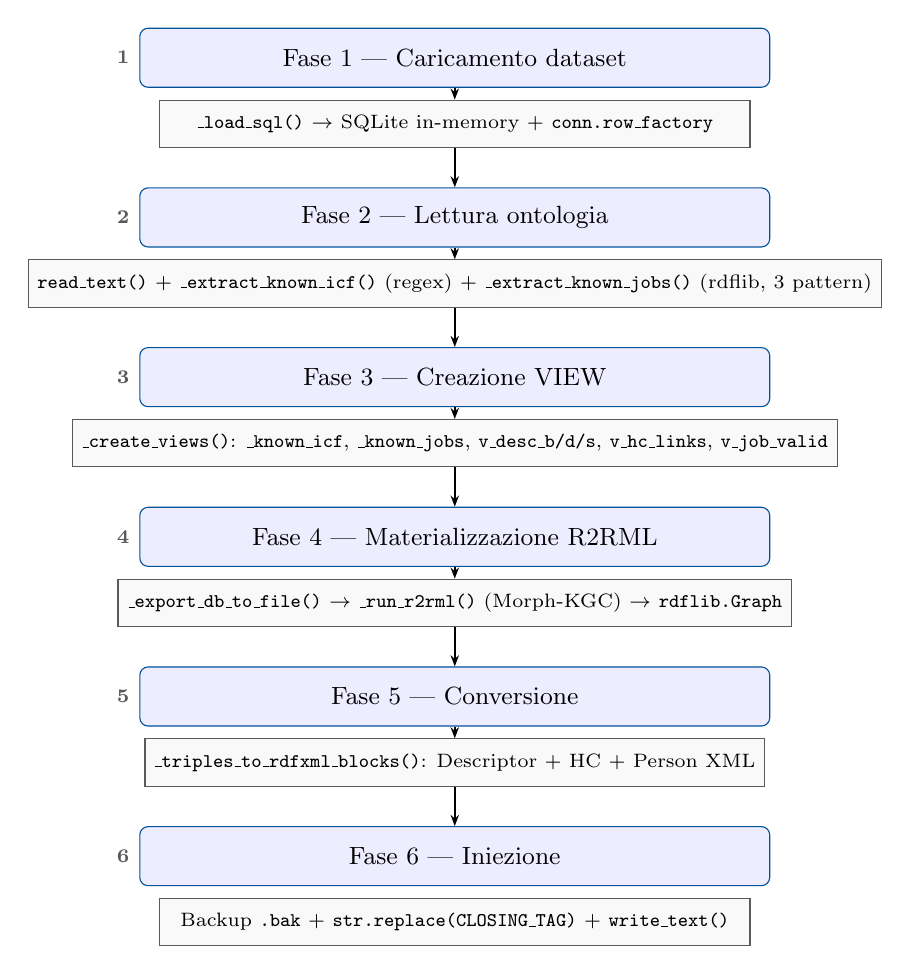
\begin{tikzpicture}[scale=0.85,
  node distance=0.7cm,
  phase/.style={rectangle, rounded corners=3pt, draw=rientraBlue,
                fill=blue!7, minimum width=8cm, minimum height=0.75cm,
                align=center, font=\small},
  detail/.style={rectangle, draw=rientraGray, fill=gray!5,
                 minimum width=7.5cm, minimum height=0.6cm,
                 align=center, font=\scriptsize},
  arrow/.style={-{Stealth[length=4pt]}, thick},
  label/.style={left, font=\scriptsize\bfseries, rientraGray},
]
  \node[phase] (p1) {Fase 1 --- Caricamento dataset};
  \node[detail, below=0.15cm of p1] (d1) {\texttt{\_load\_sql()} $\rightarrow$ SQLite in-memory + \texttt{conn.row\_factory}};

  \node[phase, below=0.5cm of d1] (p2) {Fase 2 --- Lettura ontologia};
  \node[detail, below=0.15cm of p2] (d2) {\texttt{read\_text()} + \texttt{\_extract\_known\_icf()} (regex) + \texttt{\_extract\_known\_jobs()} (rdflib, 3 pattern)};

  \node[phase, below=0.5cm of d2] (p3) {Fase 3 --- Creazione VIEW};
  \node[detail, below=0.15cm of p3] (d3) {\texttt{\_create\_views()}: \texttt{\_known\_icf}, \texttt{\_known\_jobs}, \texttt{v\_desc\_b/d/s}, \texttt{v\_hc\_links}, \texttt{v\_job\_valid}};

  \node[phase, below=0.5cm of d3] (p4) {Fase 4 --- Materializzazione R2RML};
  \node[detail, below=0.15cm of p4] (d4) {\texttt{\_export\_db\_to\_file()} $\rightarrow$ \texttt{\_run\_r2rml()} (Morph-KGC) $\rightarrow$ \texttt{rdflib.Graph}};

  \node[phase, below=0.5cm of d4] (p5) {Fase 5 --- Conversione};
  \node[detail, below=0.15cm of p5] (d5) {\texttt{\_\allowbreak{}triples\_\allowbreak{}to\_\allowbreak{}rdfxml\_\allowbreak{}blocks()}: Descriptor + HC + Person XML};

  \node[phase, below=0.5cm of d5] (p6) {Fase 6 --- Iniezione};
  \node[detail, below=0.15cm of p6] (d6) {Backup \texttt{.bak} + \texttt{str.replace(CLOSING\_TAG)} + \texttt{write\_text()}};

  \draw[arrow] (p1) -- (d1); \draw[arrow] (d1) -- (p2);
  \draw[arrow] (p2) -- (d2); \draw[arrow] (d2) -- (p3);
  \draw[arrow] (p3) -- (d3); \draw[arrow] (d3) -- (p4);
  \draw[arrow] (p4) -- (d4); \draw[arrow] (d4) -- (p5);
  \draw[arrow] (p5) -- (d5); \draw[arrow] (d5) -- (p6);

  \node[label] at (p1.west) {1};
  \node[label] at (p2.west) {2};
  \node[label] at (p3.west) {3};
  \node[label] at (p4.west) {4};
  \node[label] at (p5.west) {5};
  \node[label] at (p6.west) {6};
\end{tikzpicture}%
}% end resizebox
\caption{Pipeline completa di \texttt{import\_sql\_dataset()}.}
\end{figure}

% ============================================================
% ============================================================
\section{Layer applicativo Electron --- Struttura del progetto grafico}
% ============================================================

\subsection{Architettura generale dell'applicazione desktop}

Il frontend grafico di Rientr@ \`{e} un'applicazione desktop costruita
con \textbf{Electron} + \textbf{React} (Vite). La scelta di Electron
rispetto alle alternative \`{e} motivata da tre fattori concreti:
\begin{enumerate}
  \item \textbf{Gestione del sottoprocesso Python}: Electron espone
        \texttt{child\_process.spawn} con pieno controllo di stdin/stdout/stderr,
        pipe di logging e segnali di terminazione (\texttt{SIGTERM}).
        Framework come Tauri (Rust-based) richiedono plugin aggiuntivi
        o sidecar per gestire processi esterni con questo livello di controllo.
  \item \textbf{Ecosistema React/Node.js}: il team usa gi\`{a} React e npm.
        Electron permette di riutilizzare l'intera toolchain (Vite, TypeScript,
        ESLint) senza aggiungere un secondo linguaggio (Rust per Tauri).
  \item \textbf{API native immediate}: \texttt{dialog.showOpenDialog},
        \texttt{fs.readFileSync} e \texttt{ipcMain.handle} sono disponibili
        nativamente senza wrapper. NW.js offre funzionalit\`{a} simili ma
        con un'architettura IPC meno strutturata e un ecosistema di
        documentazione pi\`{u} limitato.
\end{enumerate}
Electron funge da \textit{host nativo} che avvolge il frontend web React
e gestisce il ciclo di vita del microservizio Python, avviandolo e terminandolo
insieme all'applicazione.

La struttura del progetto (directory \texttt{Graphic/rientra-app}),
visibile dalla struttura fornita, \`{e} organizzata come segue:

\begin{table}[H]
\centering
\caption{Struttura delle directory del progetto grafico.}
\begin{tabular}{L{4cm} L{8.5cm}}
\toprule
\textbf{Directory / File} & \textbf{Contenuto} \\
\midrule
\texttt{electron/} &
  Processo principale Electron (\texttt{main.js},
  \texttt{preload.js}). Qui risiede tutta la logica nativa:
  avvio Python, finestra, IPC, menu. \\[3pt]
\texttt{src/} &
  Sorgenti React/TypeScript del renderer (componenti, pagine,
  hook, stili). \\[3pt]
\texttt{public/} &
  Asset statici: loghi (\texttt{logo-rientra.png},
  \texttt{logo-stiima.png}, \texttt{logo-inail.png}),
  icone (\texttt{icons.svg}, \texttt{favicon.svg}),
  immagini UI (\texttt{Archive.png}, \texttt{User\_scan\_fill.png},
  \texttt{Vector.png}). \\[3pt]
\texttt{dist/} &
  Bundle di produzione generato da Vite (\texttt{vite build}),
  servito da Electron in modalit\`{a} production tramite
  \texttt{win.loadFile()}. \\[3pt]
\texttt{python-service/} &
  Directory del microservizio FastAPI (contenuto documentato
  nelle sezioni precedenti). Referenziata da \texttt{main.js}
  tramite \texttt{path.join(\_\allowbreak{}\_\allowbreak{}dirname, '..', 'python-service')}. \\[3pt]
\texttt{node\_modules/} &
  Dipendenze npm (non versionato). \\[3pt]
\texttt{package.json} &
  Manifest npm: dipendenze, script (\texttt{dev}, \texttt{build},
  \texttt{electron}), configurazione Electron Forge/Builder. \\[3pt]
\texttt{vite.config.ts} &
  Configurazione Vite per il bundle React. \\[3pt]
\texttt{tsconfig*.json} &
  Configurazioni TypeScript separate per app (\texttt{tsconfig.app.json}),
  Node (\texttt{tsconfig.node.json}) e root. \\[3pt]
\texttt{eslint.config.js} &
  Regole ESLint per il codice TypeScript/React. \\[3pt]
\texttt{index.html} &
  Entry point HTML di Vite. \\[3pt]
\texttt{start.sh} &
  Script shell di avvio rapido per lo sviluppo. \\[3pt]
\texttt{replace.js} &
  Script di utilit\`{a} per sostituzioni nel bundle (post-build). \\[3pt]
\texttt{fix\_box.py} / \texttt{restructure.py} &
  Script Python di utilit\`{a} per la gestione del layout di build. \\
\bottomrule
\end{tabular}
\end{table}

\subsection{Architettura a tre processi di Electron}

Electron separa l'applicazione in tre processi distinti con privilegi
differenti. Questa separazione non \`{e} una convenzione arbitraria ma
una scelta di sicurezza fondamentale: se il processo renderer (che carica
HTML/JS potenzialmente da sorgenti esterne) avesse accesso diretto a
Node.js, una XSS nel frontend potrebbe leggere il filesystem, avviare
processi arbitrari o accedere ai dati clinici dei pazienti. La separazione
dei privilegi garantisce che solo il Main Process (che non elabora HTML
esterno) abbia accesso alle API di sistema, e che il Preload Script agisca
come \textit{mediatore controllato} che espone \textbf{esattamente} le
operazioni necessarie e nient'altro:

\begin{figure}[htbp]
\centering
\resizebox{\linewidth}{!}{%
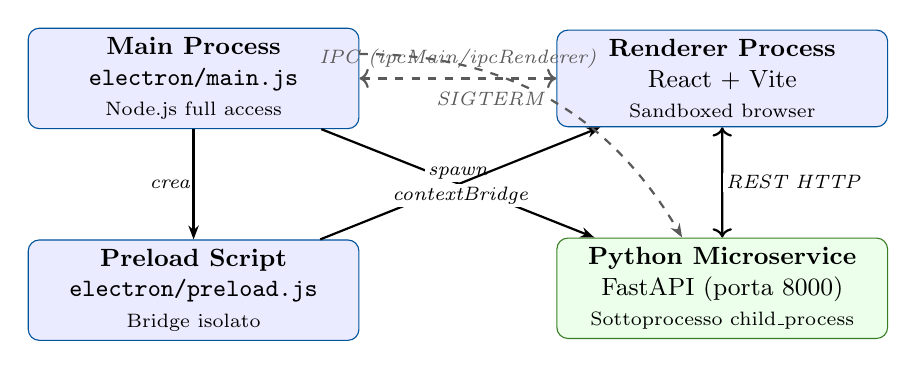
\begin{tikzpicture}[scale=0.85,
  node distance=1.2cm and 1.8cm,
  proc/.style={rectangle, rounded corners=4pt, draw=rientraBlue,
               fill=blue!8, minimum width=4.2cm, minimum height=1cm,
               align=center, font=\small},
  ext/.style={rectangle, rounded corners=4pt, draw=OliveGreen,
              fill=green!8, minimum width=4.2cm, minimum height=1cm,
              align=center, font=\small},
  arrow/.style={-{Stealth[length=5pt]}, thick},
  darrow/.style={-{Stealth[length=5pt]}, thick, dashed, rientraGray},
  lab/.style={font=\scriptsize\itshape},
]
  \node[proc] (main) {\textbf{Main Process}\\
    \texttt{electron/\allowbreak main.js}\\
    {\scriptsize Node.js full access}};

  \node[proc, right=2.5cm of main] (renderer) {\textbf{Renderer Process}\\
    React + Vite\\
    {\scriptsize Sandboxed browser}};

  \node[proc, below=1.4cm of main] (preload) {\textbf{Preload Script}\\
    \texttt{electron/\allowbreak preload.js}\\
    {\scriptsize Bridge isolato}};

  \node[ext, below=1.4cm of renderer] (python) {\textbf{Python Microservice}\\
    FastAPI (porta 8000)\\
    {\scriptsize Sottoprocesso child\_process}};

  \draw[arrow] (main) -- node[lab, above, fill=white, inner sep=1pt] {spawn} (python);
  \draw[arrow] (main) -- node[lab, left, fill=white, inner sep=1pt] {crea} (preload);
  \draw[arrow] (preload) -- node[lab, below, fill=white, inner sep=1pt] {contextBridge} (renderer);
  \draw[darrow, <->] (main) -- node[lab, above] {IPC (ipcMain/ipcRenderer)} (renderer);
  \draw[arrow, <->] (renderer) -- node[lab, right, fill=white, inner sep=1pt] {REST HTTP} (python);
  \draw[darrow, bend left=30] (main) to node[lab, left, fill=white, inner sep=1pt] {SIGTERM} (python);
\end{tikzpicture}%
}% end resizebox
\caption{Architettura a tre processi di Electron nel progetto Rientr@.}
\end{figure}

% ============================================================
\subsection{Modulo \texttt{electron/\allowbreak main.js} --- Processo principale}
% ============================================================

\subsubsection{Ruolo e responsabilit\`{a}}

\texttt{main.js} \`{e} il \textbf{processo principale} di Electron:
\`{e} l'unico processo con accesso completo a Node.js e alle API di
sistema. Ha quattro macro-responsabilit\`{a}:

\begin{enumerate}
  \item \textbf{Avvio e supervisione del microservizio Python} tramite
        \texttt{child\_process.spawn}.
  \item \textbf{Creazione e configurazione della finestra principale}
        (\texttt{BrowserWindow}).
  \item \textbf{Gestione del ciclo di vita dell'applicazione} (eventi
        \texttt{ready}, \texttt{window-all-closed}, \texttt{will-quit}).
  \item \textbf{Esposizione di API native al renderer} tramite handler
        IPC (\texttt{ipcMain.handle}).
\end{enumerate}

\subsubsection{Risoluzione dell'eseguibile Python}
\vspace{2pt}
\begin{lstlisting}[language=Java, caption={Risoluzione cross-platform dell'eseguibile Python.}]
const isWindows = process.platform === 'win32';

const VENV_PYTHON = isWindows
  ? path.join(SERVICE_DIR, '.venv', 'Scripts', 'python.exe')
  : path.join(SERVICE_DIR, '.venv', 'bin', 'python3');

const FALLBACK_PYTHON = isWindows ? 'python' : 'python3';
\end{lstlisting}

\noindent La risoluzione dell'eseguibile segue una gerarchia a due livelli:
\begin{enumerate}[noitemsep]
  \item \textbf{Virtual environment dedicato}: cerca
        \texttt{python-service/.venv/bin/python3} (Linux/macOS) o
        \texttt{.venv\textbackslash Scripts\textbackslash python.exe}
        (Windows). L'uso del venv garantisce che le dipendenze
        (\texttt{owlready2}, \texttt{fastapi}, \texttt{morph-kgc})
        siano isolate dall'ambiente di sistema.
  \item \textbf{Fallback sistema}: se il venv non esiste
        (\texttt{fs.existsSync(VENV\_\allowbreak{}PYTHON) = false}), usa il Python
        globale del sistema. Questo permette l'avvio anche senza
        un venv pre-configurato, utile in fase di sviluppo.
\end{enumerate}

La scelta di \texttt{python3} (non \texttt{python}) come fallback su
Linux/macOS \`{e} intenzionale: su questi sistemi \texttt{python}
pu\`{o} puntare a Python 2, incompatibile con il microservizio.

\subsubsection{\texttt{startPythonService()} --- Avvio del sottoprocesso}

\begin{lstlisting}[language=Java, caption={Avvio di uvicorn come sottoprocesso Node.js.}]
pythonProcess = spawn(
  pythonExe,
  ['-m', 'uvicorn', 'main:app',
   '--host', '127.0.0.1',
   '--port', String(PYTHON_PORT)],
  {
    cwd: SERVICE_DIR,
    stdio: ['ignore', 'pipe', 'pipe'],  // cattura stdout/stderr
  }
);

pythonProcess.stdout.on('data', (data) =>
  console.log('[Python]', data.toString().trim())
);
pythonProcess.stderr.on('data', (data) =>
  console.error('[Python ERR]', data.toString().trim())
);
\end{lstlisting}

\noindent \begin{infobox}[Scelta --- \texttt{spawn} vs \texttt{exec} vs \texttt{fork}]
\texttt{spawn} \`{e} preferito rispetto a \texttt{exec} perch\'{e}:
\begin{itemize}[noitemsep]
  \item Non ha limite sulla dimensione dell'output (nessun buffer overflow
        su log verbosi di Pellet).
  \item Permette di leggere stdout/stderr in streaming (\texttt{on('data')})
        per logging in tempo reale nella console Electron.
  \item Il processo figlio \`{e} un riferimento diretto, terminabile
        con \texttt{SIGTERM} preciso.
\end{itemize}
\texttt{fork} non \`{e} applicabile perch\'{e} riservato ai moduli
Node.js, non agli eseguibili Python.
\end{infobox}

\textbf{Nota sull'host:} il servizio viene avviato su \texttt{127.0.0.1}
(loopback) anzich\'{e} \texttt{0.0.0.0}. Questa scelta limita l'accesso
al solo processo locale, prevenendo esposizioni accidentali in rete in
modalit\`{a} desktop.

\textbf{Cattura degli stream}: \texttt{stdio: ['ignore', 'pipe', 'pipe']}
reindirizza stdout e stderr del processo Python verso i listener
\texttt{on('data')} di Node.js, che li prefissano con \texttt{[Python]}
e \texttt{[Python ERR]} e li emettono nella console Electron. Questo
permette il debug del microservizio direttamente dagli strumenti
di sviluppo Electron.

\subsubsection{\texttt{stopPythonService()} --- Terminazione pulita}

\begin{lstlisting}[language=Java, caption={Terminazione del sottoprocesso Python.}]
function stopPythonService() {
  if (pythonProcess) {
    pythonProcess.kill('SIGTERM');  // graceful shutdown
    pythonProcess = null;
  }
}
\end{lstlisting}

\noindent \texttt{SIGTERM} (anzich\'{e} \texttt{SIGKILL}) permette a uvicorn di
eseguire il cleanup del processo ASGI (chiusura delle connessioni HTTP
aperte, flush dei buffer di log) prima della terminazione. Il processo
Python viene terminato in due momenti del ciclo di vita Electron:
\begin{itemize}[noitemsep]
  \item \texttt{window-all-closed}: quando l'utente chiude l'ultima
        finestra (comportamento standard su Windows/Linux).
  \item \texttt{will-quit}: segnale di uscita dell'app (include il caso
        macOS dove \texttt{window-all-closed} non causa quit).
\end{itemize}
Il doppio hook garantisce che il processo Python non rimanga
\textit{zombie} in background indipendentemente dalla piattaforma.

\subsubsection{Creazione della finestra --- \texttt{createWindow()}}

\begin{lstlisting}[language=Java, caption={Configurazione della BrowserWindow principale.}]
const win = new BrowserWindow({
  width: 1280, height: 800,
  minWidth: 900, minHeight: 600,
  title: 'RIENTR@ returns -- Decision Support System',
  backgroundColor: '#1a2a4a',   // blu scuro Rientr@ (evita flash bianco)
  webPreferences: {
    preload: path.join(__dirname, 'preload.js'),
    contextIsolation: true,     // sandbox del renderer
    nodeIntegration: false,     // blocca accesso Node.js dal renderer
  },
});
\end{lstlisting}

\noindent \begin{table}[H]
\centering\small
\caption{Motivazione delle opzioni \texttt{BrowserWindow}.}
\begin{tabular}{L{4cm} L{8.5cm}}
\toprule
\textbf{Opzione} & \textbf{Motivazione} \\
\midrule
\texttt{width/height: 1280x800} &
  Risoluzione minima standard per applicazioni desktop professionali;
  sufficiente per mostrare scatter plot e tabelle di dettaglio senza scroll. \\[3pt]
\texttt{minWidth/minHeight: 900x600} &
  Soglia sotto cui i layout React collasserebbero; impedisce
  il ridimensionamento a dimensioni inutilizzabili. \\[3pt]
\texttt{backgroundColor: '\#1a2a4a'} &
  Colore di sfondo blu scuro corrispondente al tema dell'applicazione.
  Evita il ``flash bianco'' durante il caricamento del renderer. \\[3pt]
\texttt{contextIsolation: true} &
  Isola il contesto JavaScript del renderer dal contesto Node.js
  del preload. Requisito di sicurezza fondamentale in Electron
  moderno (default \texttt{true} da Electron 12). \\[3pt]
\texttt{nodeIntegration: false} &
  Impedisce al codice React di accedere direttamente alle API
  Node.js (\texttt{fs}, \texttt{path}, ecc.), prevenendo
  attacchi XSS con escalation di privilegi. \\[3pt]
\texttt{preload: preload.js} &
  Specifica lo script di bridge che espone le API native al
  renderer in modo controllato tramite \texttt{contextBridge}. \\
\bottomrule
\end{tabular}
\end{table}

\subsubsection{Dev vs Production --- caricamento dell'interfaccia}
\vspace{2pt}
\begin{lstlisting}[language=Java, caption={Caricamento condizionale dev/production.}]
const isDev = process.env.NODE_ENV === 'development';

if (isDev) {
  win.loadURL('http://localhost:5173');   // Vite dev server
} else {
  win.loadFile(path.join(__dirname, '../dist/index.html'));  // bundle
}
\end{lstlisting}

\noindent \begin{table}[H]
\centering\small
\caption{Differenze tra modalit\`{a} development e production.}
\begin{tabular}{L{3cm} L{4.5cm} L{5cm}}
\toprule
\textbf{Aspetto} & \textbf{Development} & \textbf{Production} \\
\midrule
Sorgente UI & Vite dev server (\texttt{localhost:5173}) &
  Bundle compilato (\texttt{dist/index.html}) \\
Hot reload & Si (HMR Vite) & No \\
Build necessaria & No & Si (\texttt{vite build}) \\
DevTools & Decommentare \texttt{openDevTools()} & Non disponibili \\
Distribuzione & Solo sviluppo locale & Pacchetto installabile \\
\bottomrule
\end{tabular}
\end{table}

La variabile \texttt{NODE\_ENV} viene impostata dallo script npm
di sviluppo (\texttt{"dev": "NODE\_\allowbreak{}ENV=development electron ."}),
rendendo il branch trasparente allo sviluppatore.

\subsubsection{Gestione del menu nativo}
\vspace{2pt}
\begin{lstlisting}[language=Java, caption={Rimozione del menu nativo.}]
Menu.setApplicationMenu(null);
\end{lstlisting}

\noindent Il menu nativo di sistema (File, Edit, View, ecc.) viene rimosso.
Questa scelta \`{e} tipica delle applicazioni \textit{kiosk-like} o
professionali con interfaccia custom che non richiedono le voci di
menu standard del browser. Tutta la navigazione avviene tramite
l'interfaccia React interna.

\subsubsection{Handler IPC esposti al renderer}

\begin{table}[H]
\centering\small
\caption{Handler IPC di \texttt{main.js} accessibili tramite \texttt{electronAPI}.}
\begin{tabular}{L{4.5cm} L{8cm}}
\toprule
\textbf{Canale IPC} & \textbf{Funzione e risposta} \\
\midrule
\texttt{get-python-port} &
  Restituisce la costante \texttt{PYTHON\_PORT} (8000). Permette
  al renderer di conoscere la porta del microservizio senza
  hardcodarla nel codice React. \\[3pt]
\texttt{show-open-dialog} &
  Apre il dialog nativo di selezione file del sistema operativo
  con le opzioni passate dal renderer. Restituisce
  \texttt{\{canceled, filePaths\}}.
  Usato dal pulsante ``Add Worker'' per selezionare il file
  \texttt{.sql} di import. \\[3pt]
\texttt{read-file-buffer} &
  Legge un file dal filesystem con \texttt{fs.readFileSync()}
  e lo restituisce come \texttt{\{ok, data: number[]\}}
  (array di byte serializzabile attraverso \texttt{contextBridge}).
  Permette al renderer di inviare il file SQL al microservizio
  Python via HTTP senza accesso diretto al filesystem. \\
\bottomrule
\end{tabular}
\end{table}

\begin{infobox}[Perch\'{e} \texttt{number[]} anzich\'{e} \texttt{Buffer} o \texttt{Uint8Array}]
\texttt{contextBridge} serializza i dati attraverso la boundary
di isolamento del contesto usando la \textit{Structured Clone Algorithm}.
\texttt{Buffer} (Node.js) e \texttt{Uint8Array} non sono sempre
clonabili in modo affidabile tra contesti isolati in tutte le versioni
di Electron. \texttt{Array.from(buf)} produce un \texttt{number[]}
standard, garantito serializzabile. Il renderer lo ricostruisce come
\texttt{Uint8Array} (o \texttt{Blob}) prima di inviarlo via
\texttt{fetch} al microservizio Python.
\end{infobox}

% ============================================================
\subsection{Modulo \texttt{electron/\allowbreak preload.js} --- Bridge sicuro}
% ============================================================

\subsubsection{Ruolo e principio di funzionamento}

\texttt{preload.js} \`{e} lo \textbf{script di bridge} tra il processo
principale (Node.js) e il processo renderer (React). Viene eseguito
in un contesto JavaScript isolato che ha accesso \textit{sia} alle
API Node.js \textit{sia} al DOM del renderer, ma espone al renderer
solo le API esplicitamente dichiarate tramite \texttt{contextBridge}.

\begin{lstlisting}[language=Java, caption={\texttt{preload.js} --- esposizione sicura delle API native.}]
const { contextBridge, ipcRenderer } = require('electron');

contextBridge.exposeInMainWorld('electronAPI', {
  // Info piattaforma
  platform: process.platform,

  // Dialog file picker nativo
  showOpenDialog: (options) =>
    ipcRenderer.invoke('show-open-dialog', options),

  // Lettura file come buffer di byte
  readFileBuffer: (filePath) =>
    ipcRenderer.invoke('read-file-buffer', filePath),
});
\end{lstlisting}

\noindent \subsubsection{API esposte: \texttt{window.electronAPI}}

Il codice React accede alle funzionalit\`{a} native tramite
\texttt{window.electronAPI}, che \texttt{contextBridge} rende
disponibile sul global \texttt{window} del renderer:

\begin{table}[H]
\centering\small
\caption{API disponibili in \texttt{window.electronAPI} nel renderer React.}
\begin{tabular}{L{4.2cm} L{3.8cm} L{4.5cm}}
\toprule
\textbf{Propriet\`{a}/Metodo} & \textbf{Tipo} & \textbf{Uso nel frontend} \\
\midrule
\texttt{platform} &
  \texttt{string} &
  Valore di \texttt{process.platform} (es.\ \texttt{'darwin'},
  \texttt{'win32'}, \texttt{'linux'}). Usato per logica OS-specifica
  (es.\ separatori di path, stile pulsanti). \\[3pt]
{\small\texttt{showOpenDialog(\allowbreak{}options)}} &
  {\small\texttt{Promise<\{canceled,\allowbreak{} filePaths\}>}} &
  Apre il file picker nativo per selezionare il dataset \texttt{.sql}
  da importare nel pulsante ``Add Worker''. \\[3pt]
\texttt{readFileBuffer(\allowbreak{}filePath)} &
  \texttt{Promise<\{ok, data\}>} &
  Legge il file \texttt{.sql} selezionato e lo restituisce come
  \texttt{number[]} per l'upload al microservizio Python. \\
\bottomrule
\end{tabular}
\end{table}

\subsubsection{Perch\'{e} \texttt{contextBridge} \`{e} necessario}

\begin{infobox}[Sicurezza Electron --- \texttt{contextIsolation} e \texttt{contextBridge}]
Con \texttt{contextIsolation: true} (impostato in \texttt{main.js}),
il codice JavaScript del renderer non condivide il contesto di esecuzione
con il preload. Senza \texttt{contextBridge}, il renderer non pu\`{o}
accedere a \textit{nessuna} API Node.js.

\texttt{contextBridge.exposeInMainWorld('electronAPI', \{...\})} crea un
\textbf{``tunnel''} sicuro: solo le funzioni esplicitamente elencate
nell'oggetto vengono esposte, con i valori clonati (non per riferimento)
attraverso la boundary di isolamento. Il renderer non pu\`{o} accedere
a \texttt{ipcRenderer} direttamente --- pu\`{o} solo chiamare le funzioni
pre-approvate definite in \texttt{preload.js}.

Questo pattern previene che codice JavaScript malevolo caricato
accidentalmente nel renderer (es.\ da una XSS o da una dipendenza
compromessa) possa accedere al filesystem, eseguire processi o fare
uso delle API Electron complete.
\end{infobox}

\subsubsection{Flusso di import del dataset SQL: end-to-end}

Il seguente diagramma mostra il flusso completo dell'operazione
``Add Worker'' (import di un dataset \texttt{.sql}) dall'interazione
utente fino alla risposta del microservizio:

\begin{figure}[htbp]
\centering
\resizebox{\linewidth}{!}{%
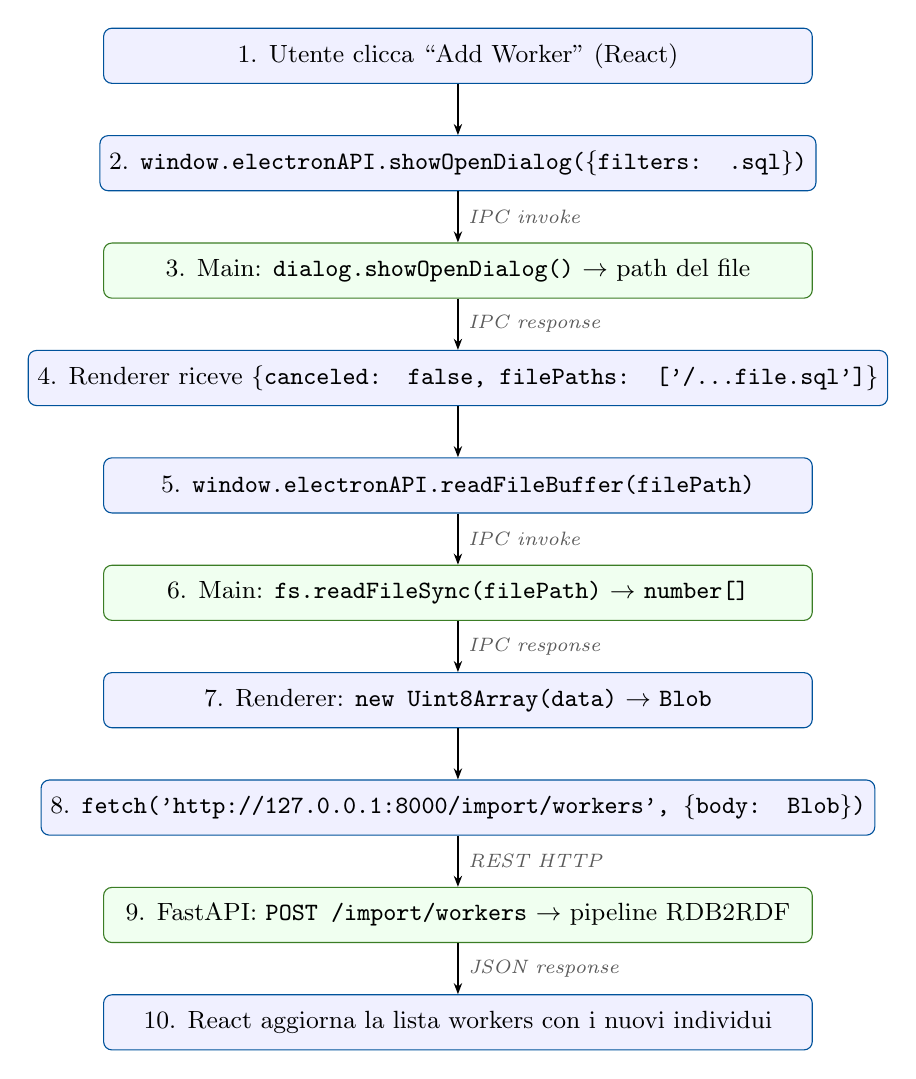
\begin{tikzpicture}[scale=0.85,
  node distance=0.65cm,
  box/.style={rectangle, rounded corners=3pt, draw=rientraBlue,
              fill=blue!6, minimum width=9cm, minimum height=0.7cm,
              align=center, font=\small},
  proc/.style={rectangle, rounded corners=3pt, draw=OliveGreen,
               fill=green!6, minimum width=9cm, minimum height=0.7cm,
               align=center, font=\small},
  arrow/.style={-{Stealth[length=4pt]}, thick},
  note/.style={right, font=\scriptsize\itshape, rientraGray},
]
  \node[box] (b1) {1. Utente clicca ``Add Worker'' (React)};
  \node[box, below=of b1] (b2)
    {2. \texttt{window.electronAPI.showOpenDialog(\{filters: .sql\})}};
  \node[proc, below=of b2] (b3)
    {3. Main: \texttt{dialog.showOpenDialog()} $\rightarrow$ path del file};
  \node[box, below=of b3] (b4)
    {4. Renderer riceve \texttt{\{canceled: false, filePaths: ['/...file.sql']\}}};
  \node[box, below=of b4] (b5)
    {5. \texttt{window.electronAPI.readFileBuffer(filePath)}};
  \node[proc, below=of b5] (b6)
    {6. Main: \texttt{fs.readFileSync(filePath)} $\rightarrow$ \texttt{number[]}};
  \node[box, below=of b6] (b7)
    {7. Renderer: \texttt{new Uint8Array(data)} $\rightarrow$ \texttt{Blob}};
  \node[box, below=of b7] (b8)
    {8. \texttt{fetch('http://127.0.0.1:8000/import/workers', \{body: Blob\})}};
  \node[proc, below=of b8] (b9)
    {9. FastAPI: \texttt{POST /import/workers} $\rightarrow$ pipeline RDB2RDF};
  \node[box, below=of b9] (b10)
    {10. React aggiorna la lista workers con i nuovi individui};

  \draw[arrow] (b1) -- (b2);
  \draw[arrow] (b2) -- (b3) node[note, pos=0.5] {IPC invoke};
  \draw[arrow] (b3) -- (b4) node[note, pos=0.5] {IPC response};
  \draw[arrow] (b4) -- (b5);
  \draw[arrow] (b5) -- (b6) node[note, pos=0.5] {IPC invoke};
  \draw[arrow] (b6) -- (b7) node[note, pos=0.5] {IPC response};
  \draw[arrow] (b7) -- (b8);
  \draw[arrow] (b8) -- (b9) node[note, pos=0.5] {REST HTTP};
  \draw[arrow] (b9) -- (b10) node[note, pos=0.5] {JSON response};
\end{tikzpicture}%
}% end resizebox
\caption{Flusso end-to-end dell'import dataset SQL da ``Add Worker''.}
\end{figure}

% ============================================================
\subsection{Ciclo di vita dell'applicazione Electron}
% ============================================================

\begin{figure}[htbp]
\centering
\resizebox{\linewidth}{!}{%
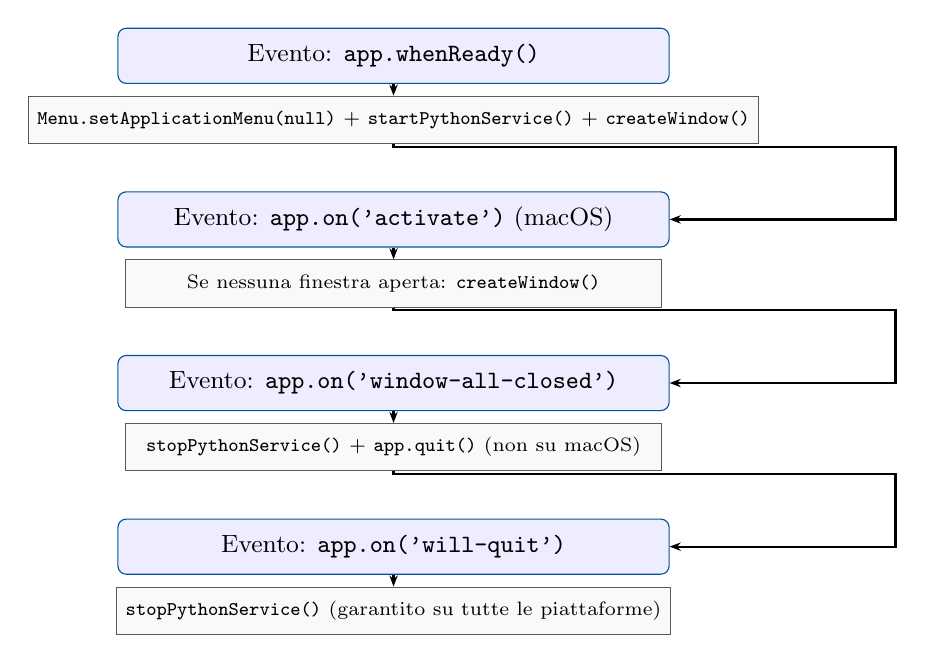
\begin{tikzpicture}[scale=0.85,
  node distance=0.8cm,
  ev/.style={rectangle, rounded corners=3pt, draw=rientraBlue,
             fill=blue!7, minimum width=7cm, minimum height=0.7cm,
             align=center, font=\small},
  act/.style={rectangle, draw=rientraGray, fill=gray!5,
              minimum width=6.8cm, minimum height=0.6cm,
              align=center, font=\scriptsize},
  arrow/.style={-{Stealth[length=4pt]}, thick},
]
  \node[ev] (e1) {Evento: \texttt{app.whenReady()}};
  \node[act, below=0.15cm of e1] (a1)
    {\texttt{Menu.setApplicationMenu(null)} + \texttt{startPythonService()} + \texttt{createWindow()}};

  \node[ev, below=0.6cm of a1] (e2) {Evento: \texttt{app.on('activate')} (macOS)};
  \node[act, below=0.15cm of e2] (a2)
    {Se nessuna finestra aperta: \texttt{createWindow()}};

  \node[ev, below=0.6cm of a2] (e3) {Evento: \texttt{app.on('window-all-closed')}};
  \node[act, below=0.15cm of e3] (a3)
    {\texttt{stopPythonService()} + \texttt{app.quit()} (non su macOS)};

  \node[ev, below=0.6cm of a3] (e4) {Evento: \texttt{app.on('will-quit')}};
  \node[act, below=0.15cm of e4] (a4)
    {\texttt{stopPythonService()} (garantito su tutte le piattaforme)};

  \draw[arrow] (e1) -- (a1);
  \draw[arrow] (a1) -- ++(0,-0.4) -- ++(7.5,0) |- (e2);
  \draw[arrow] (e2) -- (a2);
  \draw[arrow] (a2) -- ++(0,-0.4) -- ++(7.5,0) |- (e3);
  \draw[arrow] (e3) -- (a3);
  \draw[arrow] (a3) -- ++(0,-0.4) -- ++(7.5,0) |- (e4);
  \draw[arrow] (e4) -- (a4);
\end{tikzpicture}%
}% end resizebox
\caption{Ciclo di vita dell'applicazione Electron con gestione del processo Python.}
\end{figure}

La gestione del ciclo di vita macOS merita attenzione particolare:
su macOS le applicazioni non terminano quando si chiude l'ultima
finestra (il processo rimane nel Dock). L'evento \texttt{activate}
permette di riaprire la finestra cliccando sull'icona nel Dock,
mentre \texttt{will-quit} garantisce che il processo Python venga
sempre terminato anche in questo scenario.

% ============================================================
\section{Layer React --- Sorgenti \texttt{src/}}
% ============================================================

\subsection{Struttura della directory \texttt{src/}}

La directory \texttt{src/} contiene l'intera logica del frontend
React/TypeScript dell'applicazione Rientr@. La struttura, visibile
dall'albero del progetto, \`{e} organizzata in quattro livelli:

\begin{table}[H]
\centering
\caption{Struttura della directory \texttt{src/} con contenuto.}
\begin{tabular}{L{5.5cm} L{7cm}}
\toprule
\textbf{Path} & \textbf{Contenuto} \\
\midrule
\texttt{src/main.tsx} &
  Entry point React: monta \texttt{<App/>} in \texttt{\#root}. \\[3pt]
\texttt{src/App.tsx} &
  Root component: routing client-side tra \texttt{HomePage}
  e \texttt{WorkersPage}, gestione dello stato di navigazione. \\[3pt]
\texttt{src/index.css} &
  Reset CSS globale, font, user-select, drag prevention. \\[3pt]
\texttt{src/App.css} &
  Stili legacy del template Vite (contatore, hero, next-steps).
  Presente ma non attivamente usato dall'UI di produzione. \\[3pt]
\texttt{src/api/} &
  Layer di accesso al microservizio Python. \\[3pt]
\texttt{src/api/\allowbreak{}semanticService.ts} &
  Tutte le chiamate REST al microservizio FastAPI (porta 8000). \\[3pt]
\texttt{src/assets/} &
  Asset statici importati da Vite: \texttt{hero.png},
  \texttt{react.svg}, \texttt{vite.svg}. \\[3pt]
\texttt{src/components/} &
  Componenti React principali dell'applicazione. \\[3pt]
\texttt{src/\allowbreak{}components/\allowbreak{}HomePage.tsx} / \texttt{.css} &
  Schermata di benvenuto con navigazione ai moduli. \\[3pt]
\texttt{src/components/\allowbreak{}WorkersPage.tsx} / \texttt{.css} &
  Dashboard principale: lista workers, matching, dettaglio. \\[3pt]
\texttt{src/\allowbreak{}components/\allowbreak{}JobAnalysis\allowbreak{}View.tsx} / \texttt{.css} &
  Vista analisi job: scatter plot, importanza skill, profilo. \\[3pt]
\texttt{src/\allowbreak{}components/\allowbreak{}HealthCondition\allowbreak{}Wizard.tsx} / \texttt{.css} &
  Procedura guidata per la modifica delle condizioni ICF. \\
\bottomrule
\end{tabular}
\end{table}

\begin{figure}[htbp]
\centering
\resizebox{\linewidth}{!}{%
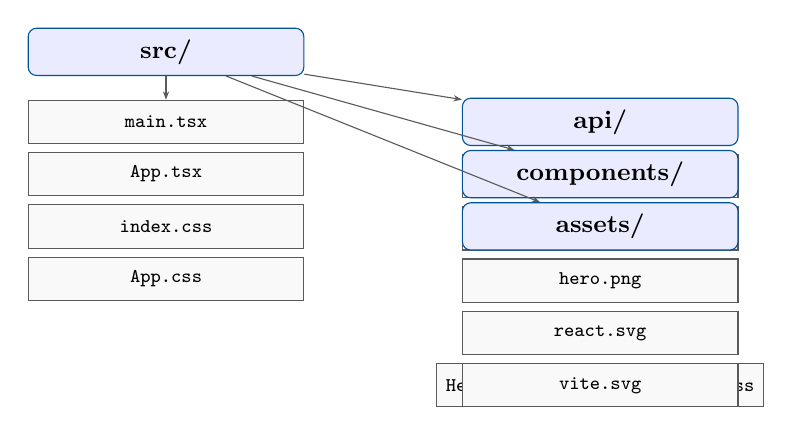
\begin{tikzpicture}[scale=0.85,
  node distance=0.55cm and 1.6cm,
  dir/.style={rectangle, rounded corners=3pt, draw=rientraBlue,
              fill=blue!8, minimum width=3.5cm, minimum height=0.6cm,
              align=center, font=\small\bfseries},
  file/.style={rectangle, draw=rientraGray, fill=gray!5,
               minimum width=3.5cm, minimum height=0.55cm,
               align=center, font=\ttfamily\scriptsize},
  arrow/.style={-{Stealth[length=3pt]}, thin, rientraGray},
]
  \node[dir] (src) {src/};

  \node[file, below=0.3cm of src] (main) {main.tsx};
  \node[file, below=0.1cm of main] (app) {App.tsx};
  \node[file, below=0.1cm of app] (icss) {index.css};
  \node[file, below=0.1cm of icss] (acss) {App.css};

  \node[dir, right=2cm of main] (api) {api/};
  \node[file, below=0.1cm of api] (svc) {semanticService.ts};

  \node[dir, right=2cm of app] (comp) {components/};
  \node[file, below=0.1cm of comp] (hp) {HomePage.tsx/.css};
  \node[file, below=0.1cm of hp] (wp) {WorkersPage.tsx/.css};
  \node[file, below=0.1cm of wp] (ja) {JobAnalysisView.tsx/.css};
  \node[file, below=0.1cm of ja] (hcw) {HealthConditionWizard.tsx/.css};

  \node[dir, right=2cm of icss] (assets) {assets/};
  \node[file, below=0.1cm of assets] (hero) {hero.png};
  \node[file, below=0.1cm of hero] (rsvg) {react.svg};
  \node[file, below=0.1cm of rsvg] (vsvg) {vite.svg};

  \draw[arrow] (src) -- (main);
  \draw[arrow] (src) -- (api);
  \draw[arrow] (src) -- (comp);
  \draw[arrow] (src) -- (assets);
\end{tikzpicture}%
}% end resizebox
\caption{Struttura ad albero della directory \texttt{src/}.}
\end{figure}

% ============================================================
\subsection{\texttt{src/main.tsx} --- Entry point React}
% ============================================================

\begin{lstlisting}[caption={\texttt{main.tsx} --- montaggio dell'applicazione React.}]
import { StrictMode } from 'react'
import { createRoot } from 'react-dom/client'
import './index.css'
import App from './App.tsx'

createRoot(document.getElementById('root')!).render(
  <StrictMode>
    <App />
  </StrictMode>,
)
\end{lstlisting}

\noindent \texttt{main.tsx} \`{e} il punto di ingresso del renderer React.
Vite lo individua tramite la dichiarazione \texttt{<script type="module"
src="/src/main.tsx">} in \texttt{index.html}.

\subsubsection{Scelte implementative}

\paragraph{\texttt{StrictMode}}
Il wrapping in \texttt{React.StrictMode} attiva controlli aggiuntivi
di React in fase di sviluppo:
\begin{itemize}[noitemsep]
  \item Rileva side effect impuri nei componenti (doppia invocazione
        intenzionale dei render in dev).
  \item Segnala l'uso di API deprecate.
  \item Evidenzia componenti che non gestiscono correttamente il cleanup
        degli effect.
\end{itemize}
In produzione (\texttt{vite build}), \texttt{StrictMode} non ha impatto
sulle prestazioni: i comportamenti extra vengono rimossi dal tree-shaking.

\paragraph{\texttt{createRoot} e React 18}
L'uso di \texttt{createRoot} (anzich\'{e} il legacy \texttt{ReactDOM.render})
abilita il \textbf{Concurrent Mode} di React 18, che permette al
motore di rendering di interrompere e riprendere i render per mantenere
l'interfaccia reattiva durante operazioni costose (es.\ aggiornamenti
lista workers, rendering scatter plot).

\paragraph{Asserzione non-null \texttt{!}}
\texttt{document.getElementById('root')!} usa l'operatore TypeScript
di asserzione non-null. L'elemento \texttt{\#root} \`{e} garantito
presente dall'\texttt{index.html} generato da Vite; il \texttt{!}
evita un controllo \texttt{null} ridondante che TypeScript
richiederebbe altrimenti.

\paragraph{Import di \texttt{index.css}}
L'import del CSS globale in \texttt{main.tsx} (anzich\'{e} in
\texttt{App.tsx}) garantisce che il reset e il font siano applicati
\textbf{prima} del render del primo componente, eliminando
il flash di stile non stilizzato (FOUC).

% ============================================================
\subsection{\texttt{src/App.tsx} --- Root component e routing}
% ============================================================

\begin{lstlisting}[caption={\texttt{App.tsx} --- routing client-side e gestione navigazione.}]
import { useState } from 'react'
import './index.css'
import HomePage from './components/HomePage'
import WorkersPage from './components/WorkersPage'

type Page = 'home' | 'workers'
export type NavTarget = 'workers' | 'jobs-analysis' | 'jobs-positions'

function App() {
  const [page, setPage]           = useState<Page>('home')
  const [initialNav, setInitialNav] = useState<NavTarget>('workers')

  if (page === 'workers') {
    return <WorkersPage
      onNavigateHome={() => setPage('home')}
      initialNav={initialNav}
    />
  }

  return <HomePage onNavigate={(id) => {
    if (id === 'worker-information') {
      setInitialNav('workers'); setPage('workers');
    } else if (id === 'job-analysis') {
      setInitialNav('jobs-analysis'); setPage('workers');
    } else if (id === 'job-positions') {
      setInitialNav('jobs-positions'); setPage('workers');
    }
  }} />
}

export default App
\end{lstlisting}

\noindent \subsubsection{Pattern di routing senza React Router}

\texttt{App.tsx} implementa un routing client-side \textbf{custom}
basato su \texttt{useState} anzich\'{e} una libreria dedicata come
React Router. Questa scelta \`{e} motivata da:

\begin{itemize}
  \item \textbf{Semplicit\`{a} strutturale}: l'applicazione ha solo
        due pagine principali (\texttt{HomePage} e \texttt{WorkersPage}).
        React Router introdurrebbe overhead di configurazione e dipendenze
        per un caso d'uso cos\`{\i} lineare.
  \item \textbf{Applicazione desktop Electron}: non essendo un'app web
        con URL navigabili, non c'`{e} bisogno di sincronizzare lo stato
        della navigazione con la URL del browser. Il concetto di
        ``deep link'' e ``back button del browser'' non si applica.
  \item \textbf{Stato di navigazione trasparente}: il parametro
        \texttt{initialNav} permette di aprire \texttt{WorkersPage}
        direttamente in una delle sue tre sotto-viste
        (\texttt{workers}, \texttt{jobs-analysis}, \texttt{jobs-positions})
        senza ulteriori livelli di routing.
\end{itemize}

\subsubsection{Tipi esportati}
\vspace{2pt}
\begin{lstlisting}[caption={Tipi TypeScript esportati da \texttt{App.tsx}.}]
type Page = 'home' | 'workers'           // privato ad App
export type NavTarget =
  | 'workers'
  | 'jobs-analysis'
  | 'jobs-positions'
\end{lstlisting}

\noindent \texttt{NavTarget} \`{e} esportato (\texttt{export type}) perch\'{e}
viene usato come tipo del prop \texttt{initialNav} di
\texttt{WorkersPage}. Definirlo in \texttt{App.tsx} (l'unico posto
che lo istanzia) anzich\'{e} in un file \texttt{types.ts} separato
mantiene la dipendenza vicina al suo utilizzo principale, riducendo
l'accoppiamento tra file.

\subsubsection{Flusso di navigazione}

\begin{figure}[htbp]
\centering
\resizebox{\linewidth}{!}{%
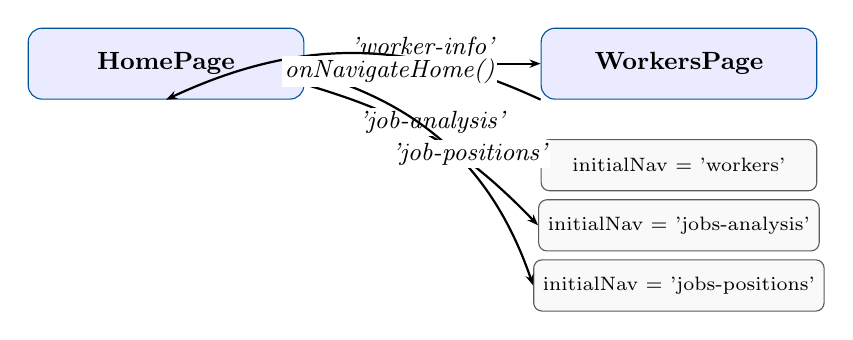
\begin{tikzpicture}[scale=0.85,
  node distance=1cm and 2.2cm,
  page/.style={rectangle, rounded corners=5pt, draw=rientraBlue,
               fill=blue!8, minimum width=3.5cm, minimum height=0.9cm,
               align=center, font=\small\bfseries},
  nav/.style={rectangle, rounded corners=3pt, draw=rientraGray,
              fill=gray!5, minimum width=3.5cm, minimum height=0.65cm,
              align=center, font=\scriptsize},
  arrow/.style={-{Stealth[length=4pt]}, thick},
  lab/.style={font=\scriptsize\itshape, above},
  labd/.style={font=\scriptsize\itshape, below},
]
  \node[page] (home) {HomePage};

  \node[page, right=3cm of home] (workers) {WorkersPage};
  \node[nav, below=0.5cm of workers] (nav1) {initialNav = 'workers'};
  \node[nav, below=0.1cm of nav1] (nav2) {initialNav = 'jobs-analysis'};
  \node[nav, below=0.1cm of nav2] (nav3) {initialNav = 'jobs-positions'};

  \draw[arrow] (home) -- node[lab, above, fill=white, inner sep=1pt]
    {\small\textit{'worker-info'}} (workers);
  \draw[arrow, bend left=15] (home) to
    node[lab, above, pos=0.5, fill=white, inner sep=1pt]
    {\small\textit{'job-analysis'}} (nav2.west);
  \draw[arrow, bend left=28] (home) to
    node[lab, above, pos=0.6, fill=white, inner sep=1pt]
    {\small\textit{'job-positions'}} (nav3.west);
  \draw[arrow, bend right=25] (workers.south west) to
    node[labd, pos=0.4, fill=white, inner sep=1pt]
    {\small\textit{onNavigateHome()}} (home.south);
\end{tikzpicture}%
}% end resizebox
\caption{Flusso di navigazione gestito da \texttt{App.tsx}.}
\end{figure}

\texttt{WorkersPage} riceve \texttt{initialNav} come prop e lo usa
per impostare la sotto-vista attiva al momento del montaggio.
La navigazione inversa (\texttt{onNavigateHome}) imposta \texttt{page}
a \texttt{'home'}, smontando \texttt{WorkersPage} e rimontando
\texttt{HomePage}, con reset automatico di tutto lo stato locale
(lista workers caricata, worker selezionato, cache delle query).

\subsubsection{Tre punti di ingresso alla \texttt{WorkersPage}}

I tre ID di navigazione corrispondono alle sezioni della \texttt{WorkersPage}:

\begin{table}[H]
\centering
\caption{Mapping ID navigazione $\rightarrow$ vista iniziale in \texttt{WorkersPage}.}
\begin{tabular}{L{4cm} L{3.5cm} L{5cm}}
\toprule
\textbf{ID (da HomePage)} & \textbf{NavTarget} & \textbf{Vista aperta} \\
\midrule
{\small\texttt{'worker-information'}} & {\small\texttt{'workers'}} &
  Tab workers: lista pazienti, selezione, condizioni ICF. \\
\texttt{'job-analysis'} & \texttt{'jobs-analysis'} &
  Vista analisi job: scatter plot GCS/AISA, importanza skill. \\
\texttt{'job-positions'} & \texttt{'jobs-positions'} &
  Vista posizioni job: profilo O*NET, radar chart. \\
\bottomrule
\end{tabular}
\end{table}

% ============================================================
\subsection{\texttt{src/index.css} --- Reset e stili globali}
% ============================================================

\begin{lstlisting}[caption={\texttt{index.css} --- CSS globale dell'applicazione.}]
@import url('https://fonts.googleapis.com/css2?
  family=Inter:wght@300;400;500;600;700;800&display=swap');

*, *::before, *::after {
  box-sizing: border-box;
  margin: 0;
  padding: 0;
}
html, body, #root { height: 100%; width: 100%; }
body {
  font-family: 'Inter', sans-serif;
  -webkit-font-smoothing: antialiased;
  -webkit-user-select: none;
  user-select: none;
}
input, textarea { -webkit-user-select: auto; user-select: auto; }
img { -webkit-user-drag: none; }
\end{lstlisting}

\noindent \subsubsection{Scelte implementative}

\paragraph{Font Inter via Google Fonts}
Il font \textbf{Inter} (pesi 300--800) \`{e} importato via CDN Google
Fonts. Inter \`{e} un typeface sans-serif ottimizzato per la leggibilit\`{a}
su schermo a basse risoluzioni, ideale per interfacce desktop con
dense tabelle di dati come quelle di Rientr@. L'import via CDN \`{e}
accettabile in un'app desktop con accesso internet garantito; per deploy
completamente offline andrebbe bundlato localmente.

\paragraph{Box model universale}
\texttt{box-sizing: border-box} su tutti gli elementi (\texttt{*},
\texttt{::before}, \texttt{::after}) garantisce che \texttt{padding}
e \texttt{border} siano inclusi nelle dimensioni dichiarate, eliminando
la fonte pi\`{u} comune di layout inconsistenti in CSS.

\paragraph{Full-height layout}
\texttt{height: 100\%} e \texttt{width: 100\%} su \texttt{html},
\texttt{body} e \texttt{\#root} permettono ai componenti React di
usare \texttt{height: 100\%} o \texttt{min-height: 100vh} per occupare
l'intera area della finestra Electron senza scrollbar verticali
indesiderate.

\paragraph{User-select disabilitato globalmente}
\texttt{-webkit-user-select: none} e \texttt{user-select: none}
sul \texttt{body} impediscono la selezione accidentale del testo
nell'interfaccia, comportamento atteso nelle applicazioni desktop
(vs.\ web). Viene ri-abilitato selettivamente su \texttt{input} e
\texttt{textarea}, dove la selezione del testo \`{e} funzionale.

\paragraph{Drag prevention sulle immagini}
\texttt{-webkit-user-drag: none} su \texttt{img} impedisce il
trascinamento nativo delle immagini fuori dall'applicazione,
che in un contesto Electron causerebbe comportamenti imprevedibili
(apertura del file nel sistema operativo).

\paragraph{Font smoothing}
\texttt{-webkit-font-smoothing: antialiased} e
\texttt{-moz-osx-font-smoothing: grayscale} attivano il rendering
subpixel del font su macOS e Firefox, producendo testo pi\`{u}
nitido. Particolarmente rilevante per Inter che \`{e} progettato
per funzionare bene con l'antialiasing.

\subsection{\texttt{src/App.css} --- Stili legacy del template Vite}

\texttt{App.css} contiene gli stili del template di default generato
da \texttt{npm create vite@latest} con il preset
\texttt{react-ts}. Include classi per il contatore interattivo
(\texttt{.counter}), l'hero image animata (\texttt{.hero}),
la sezione ``next steps'' (\texttt{\#next-steps}) e il separatore
(\texttt{\#spacer}).

Questi stili \textbf{non sono attivamente usati} dall'interfaccia
di produzione di Rientr@: il file \`{e} presente come eredit\`{a}
del bootstrap del progetto con Vite. L'import di \texttt{App.css}
in \texttt{App.tsx} \`{e} stato rimosso (si vede che \texttt{App.tsx}
importa solo \texttt{index.css}), rendendo di fatto le classi
inutilizzate. Il file pu\`{o} essere eliminato in una futura pulizia
del progetto senza impatto funzionale.

\begin{infobox}[Nota sulle CSS Nesting Rules in \texttt{App.css}]
\texttt{App.css} usa la sintassi di \textbf{CSS Nesting} nativa
(es.\ \texttt{\&:hover \{ ... \}} dentro \texttt{.counter}) che
\`{e} supportata nativamente da Vite/PostCSS senza plugin aggiuntivi
nei browser moderni (Chrome 112+, Firefox 117+, Safari 16.5+).
In Electron (basato su Chromium), questa sintassi \`{e} garantita
funzionante dalla versione di Chromium bundlata.
\end{infobox}


% ============================================================
\subsection[\texttt{src/components/HomePage.tsx} e \texttt{HomePage.css}]{\texttt{src/components/HomePage.tsx}\\[2pt]e \texttt{HomePage.css}}
% ============================================================

\subsubsection{Struttura del file e responsabilit\`{a}}

\texttt{HomePage.tsx} (133 righe) \`{e} il componente di landing
dell'applicazione. Importa esclusivamente il proprio CSS
(\texttt{HomePage.css}) e non dipende da nessun hook React di stato,
n\'{e} da API esterne: \`{e} un componente \textbf{puramente presentazionale}.

La sua interfaccia TypeScript \`{e} minimale per design:

\begin{lstlisting}
interface HomePageProps {
  onNavigate?: (cardId: string) => void;
}
\end{lstlisting}

\noindent \texttt{onNavigate} \`{e} opzionale (\texttt{?}): il componente pu\`{o}
renderizzarsi in isolamento per test o Storybook senza prop obbligatorie.
Il callback riceve l'\texttt{id} della card cliccata come stringa e lo
propaga a \texttt{App.tsx} che esegue il routing.

\subsubsection{Il tipo \texttt{NavCard} e l'array \texttt{cards}}

\begin{lstlisting}
interface NavCard {
  id:          string;
  icon:        React.ReactNode;
  title:       string;
  description: string[];
}

const cards: NavCard[] = [
  { id: 'worker-information', icon: <WorkerIcon />, title: 'Worker Information',
    description: ['Add new worker,', 'Check current health conditions,',
                  'Modify health conditions'] },
  { id: 'job-analysis', icon: <JobAnalysisIcon />, title: 'Job Analysis',
    description: ['Check and compare job opportunities for workers,',
                  'List possible work improving aids'] },
  { id: 'job-positions', icon: <JobPositionsIcon />, title: 'Job Positions',
    description: ['Check jobs, Import new jobs'] },
];
\end{lstlisting}

\noindent L'array \texttt{cards} \`{e} dichiarato \textbf{a livello di modulo},
fuori dal corpo del componente. Questa scelta \`{e} intenzionale: in React
ogni variabile dichiarata dentro un componente viene ricreata ad ogni
render. Poich\'{e} ogni elemento \texttt{icon} \`{e} un
\texttt{React.ReactNode} (JSX), il runtime React creerebbe nuovi oggetti
a ogni render senza alcuna utilit\`{a}. Dichiararli fuori dalla funzione
li rende costanti condivise nell'intera vita del modulo.

Il tipo \texttt{description: string[]} anzich\'{e} una singola stringa
permette di spezzare ogni card in pi\`{u} righe di testo senza markup
HTML inline, rendendo il contenuto modificabile direttamente nell'array
senza toccare il template JSX.

\subsubsection{Icone SVG inline --- componenti funzionali}

Le tre icone (\texttt{WorkerIcon}, \texttt{JobAnalysisIcon},
\texttt{JobPositionsIcon}) sono componenti funzionali React che
restituiscono SVG puro. La scelta di SVG inline rispetto a immagini
\texttt{<img src=".svg">} \`{e} motivata da quattro ragioni:

\begin{enumerate}
  \item \textbf{Nessuna richiesta HTTP}: in un contesto Electron con
        possibile modalit\`{a} offline, eliminare fetch di asset \`{e}
        preferibile. Vite bundla le importazioni statiche, ma il pattern
        \texttt{mask-image: url(/file.png)} usato altrove nel progetto
        richiede comunque che il file esista in \texttt{/public}.
        SVG inline non ha questa dipendenza.
  \item \textbf{Renderizzazione nitida a qualsiasi DPI}: il \texttt{viewBox}
        dell'SVG garantisce scaling vettoriale perfetto su display Retina
        e HiDPI senza pixelazione, a differenza dei PNG.
  \item \textbf{Colorabilit\`{a} via props}: le forme usano colori hardcoded
        semanticamente significativi (\texttt{\#4DD9C0} teal principale,
        \texttt{white}, \texttt{\#60C8B0} variante) che possono essere
        parametrizzati tramite prop in futuro senza modificare file esterni.
  \item \textbf{Composizione semantica}: ogni icona \`{e} costruita da primitive
        SVG (\texttt{circle}, \texttt{path}, \texttt{rect}, \texttt{line})
        che documentano visivamente la struttura
        (es.\ \texttt{WorkerIcon}: due cerchi (persone) + \texttt{rect}
        (tessera ID); \texttt{JobAnalysisIcon}: persona + lavagna con
        chart; \texttt{JobPositionsIcon}: persona + valigetta con badge ``+'').
\end{enumerate}

\subsubsection{Layout e struttura JSX}

Il componente \`{e} strutturato in tre aree semantiche HTML:

\begin{lstlisting}
<div className="home-page">         {/* wrapper radice */}
  {/* 1. Background animato */}
  <div className="bg-blob bg-blob-1" />
  <div className="bg-blob bg-blob-2" />
  <div className="bg-blob bg-blob-3" />

  {/* 2. Header brand */}
  <header className="home-header">
    <div className="brand">
      <img src="/logo-rientra.png" ... className="brand-logo" />
      <div className="brand-text">
        <span className="brand-title">RIENTR@ returns</span>
        <span className="brand-subtitle">Decision Support System</span>
      </div>
    </div>
  </header>

  {/* 3. Grid delle card */}
  <main className="home-main">
    <div className="cards-grid">
      {cards.map((card) => (
        <button key={card.id} className="nav-card"
          id={card.id} aria-label={card.title}
          onClick={() => onNavigate?.(card.id)}>
          <div className="card-icon-wrapper">{card.icon}</div>
          <div className="card-body">
            <h2 className="card-title">{card.title}</h2>
            <div className="card-divider" />
            <ul className="card-description">
              {card.description.map((line, i) => <li key={i}>{line}</li>)}
            </ul>
          </div>
          <div className="card-hover-shine" />
        </button>
      ))}
    </div>
  </main>

  {/* 4. Footer istituzionale */}
  <footer className="home-footer">
    <div className="footer-logos">
      <img src="/logo-stiima.png" ... className="footer-logo footer-logo-stiima" />
      <img src="/logo-inail.png"  ... className="footer-logo footer-logo-inail" />
    </div>
  </footer>
</div>
\end{lstlisting}

\noindent \paragraph{Card come \texttt{<button>} HTML}
Le card sono \texttt{<button>} e non \texttt{<div>} cliccabili. Questo
garantisce accessibilit\`{a} nativa senza attributi aggiuntivi:
focalizzazione con \texttt{Tab}, attivazione con \texttt{Enter}/\texttt{Space},
\texttt{role="button"} implicito letto dagli screen reader.
L'\texttt{aria-label} trasmette il nome della destinazione (es.\
\textit{``Worker Information''}) che \`{e} pi\`{u} informativo del
contenuto testuale della card.

\paragraph{Optional chaining su \texttt{onNavigate?.()}}
L'invocazione \texttt{onNavigate?.(card.id)} usa l'optional chaining
di TypeScript: se la prop non viene passata (rendering isolato), la
chiamata viene saltata silenziosamente senza errore runtime.

\paragraph{Footer: filtro CSS per loghi monocromatici}
I loghi STIIMA-CNR e INAIL vengono resi bianchi tramite
\texttt{filter: brightness(0) invert(1)} CSS, indipendentemente dal
colore originale del file PNG. Questo evita di dover mantenere versioni
bianche separate degli asset.

\subsubsection{\texttt{HomePage.css} --- sistema visivo}

\paragraph{Sfondo gradient fisso}
\vspace{2pt}
\begin{lstlisting}[language={}]
.home-page {
  background: linear-gradient(135deg,
    #1a2a4a 0%, #1e3a5f 25%, #1a4a5a 50%,
    #163860 75%, #102840 100%);
}
\end{lstlisting}
Il gradiente diagonale (135deg) usa quattro stop di blu-petrolio che
definiscono la palette cromatica dell'intera applicazione. Lo stesso
sfondo di base (\texttt{\#1a2a4a}) \`{e} usato come \texttt{backgroundColor}
in \texttt{BrowserWindow} di Electron, evitando il ``flash bianco''
durante il caricamento iniziale del renderer.

\paragraph{Blob animati}
\vspace{2pt}
\begin{lstlisting}[language={}]
.bg-blob { filter: blur(80px); opacity: 0.35;
  animation: blobDrift 12s ease-in-out infinite alternate; }

@keyframes blobDrift {
  0%   { transform: translate(0,0) scale(1); }
  33%  { transform: translate(30px,-20px) scale(1.05); }
  66%  { transform: translate(-20px,30px) scale(0.95); }
  100% { transform: translate(20px,20px) scale(1.02); }
}
\end{lstlisting}

\noindent Tre ellissi radiali con colori diversi (teal \texttt{\#4a90b8},
viola \texttt{\#6a5acd}, verde-acqua \texttt{\#20b2aa}) vengono
sfocate a 80px e animate con \texttt{blobDrift}. Le tre istanze
hanno durate diverse (14s, 10s, 16s) e \texttt{animation-delay}
sfasati (-4s, -8s), rendendo il movimento non ciclico e ``organico''.
\texttt{infinite alternate} inverte la direzione a ogni ciclo evitando
i salti visivi che si avrebbero con \texttt{infinite normal}.

\paragraph{Effetto frosted glass sulle card}
\vspace{2pt}
\begin{lstlisting}[language={}]
.nav-card {
  background: rgba(255,255,255,0.08);
  border: 1px solid rgba(255,255,255,0.2);
  backdrop-filter: blur(10px);
  -webkit-backdrop-filter: blur(10px);
  min-height: 420px;
}
\end{lstlisting}

\noindent \texttt{backdrop-filter: blur(10px)} richiede il prefisso
\texttt{-webkit-} per le versioni di Chromium bundlate in Electron
precedenti alla 76. L'effetto \`{e} visibile dove le card si sovrappongono
ai blob colorati retrostanti: il vetro smerigliato sfuma il colore del
blob mantenendo leggibilit\`{a} del testo sovrapposto.

\paragraph{Hover multi-layer con spring curve}
\vspace{2pt}
\begin{lstlisting}[language={}]
.nav-card {
  transition: transform 0.25s cubic-bezier(0.34,1.56,0.64,1),
              box-shadow 0.25s ease, background 0.25s ease,
              border-color 0.25s ease;
}
.nav-card:hover {
  transform: translateY(-6px) scale(1.02);
  background: rgba(255,255,255,0.14);
  border-color: rgba(255,255,255,0.4);
  box-shadow:
    0 12px 40px rgba(0,0,0,0.35),
    0 0 0 1px rgba(255,255,255,0.15),
    inset 0 1px 0 rgba(255,255,255,0.2);
}
.card-hover-shine { opacity: 0; transition: opacity 0.3s; }
.nav-card:hover .card-hover-shine { opacity: 1; }
\end{lstlisting}

\noindent La curva \texttt{cubic-bezier(0.34, 1.56, 0.64, 1)} \`{e} una
\textit{spring curve} con overshooting (il secondo valore $> 1$): la
card sale leggermente oltre la posizione finale prima di assestarsi,
simulando un molla. Il \texttt{box-shadow} usa tre livelli: ombra
principale sotto la card, outline esterno sottile, evidenziazione
interna sul bordo superiore (luce simulata dall'alto). Il
\texttt{card-hover-shine} \`{e} un div \texttt{absolute} con gradiente
diagonale che simula un riflesso di luce superficiale.

% ============================================================
\subsection[\texttt{src/components/WorkersPage.tsx} e \texttt{WorkersPage.css}]{\texttt{src/components/WorkersPage.tsx}\\[2pt]e \texttt{WorkersPage.css}}
% ============================================================

\subsubsection{Ruolo, dimensioni e dipendenze}

\texttt{WorkersPage.tsx} (1243 righe) \`{e} il componente pi\`{u} complesso
del frontend. Dipende da:
\begin{itemize}[noitemsep]
  \item Hook React: \texttt{useState} (15 istanze), \texttt{useEffect} (6),
        \texttt{useCallback} (1), \texttt{useRef} (2).
  \item API layer: 6 funzioni da \texttt{semanticService.ts}
        (\texttt{fetchStatus}, \texttt{fetchWorkers},
        \texttt{fetchHealthConditions}, \texttt{fetchCoreSets},
        \texttt{selectWorker}, \texttt{importWorkers}).
  \item Componenti figlio: \texttt{JobAnalysisView} e
        \texttt{HealthConditionWizard}.
  \item API nativa Electron: \texttt{window.electronAPI}
        (\texttt{showOpenDialog}, \texttt{readFileBuffer}).
\end{itemize}

\subsubsection{Icone SVG inline del componente}

\texttt{WorkersPage} definisce 10 componenti icona inline:
\texttt{SearchIcon}, \texttt{ListIcon}, \texttt{PlusIcon},
\texttt{EditIcon}, \texttt{DotsIcon}, \texttt{PdfIcon},
\texttt{RefreshIcon}, \texttt{FilterIcon}, \texttt{ArrowRightIcon},
\texttt{XIcon}. Le icone SVG seguono lo stesso pattern di
\texttt{HomePage}: stroke-based su \texttt{currentColor}, dimensioni
fisse in pixel, zero dipendenze da librerie esterne.

\texttt{ArchiveIcon} adotta invece il pattern CSS \texttt{maskImage}:
\begin{lstlisting}
const ArchiveIcon = () => (
  <span style={{
    backgroundColor: 'currentColor',
    maskImage: 'url(/Archive.png)',
    WebkitMaskImage: 'url(/Archive.png)',
    maskSize: 'contain', maskRepeat: 'no-repeat',
    maskPosition: 'center', width: 16, height: 16,
  }} />
);
\end{lstlisting}
Il quadrato colorato con \texttt{backgroundColor: 'currentColor'}
viene ritagliato dalla forma del PNG di archivio tramite CSS mask.
Questo permette di ricolorare l'icona via CSS \texttt{color} ereditato
dal genitore. Il pattern \`{e} usato anche per le icone empty-state
(\texttt{Vector.png}, \texttt{User\_scan\_fill.png}) con dimensioni
maggiori (64px).

\subsubsection{Parser \texttt{parseConditionDescription}}

\begin{lstlisting}
function parseConditionDescription(description: string): ParsedDescription {
  const normalized = (description || '').replace(/\r\n/g, '\n').trim();
  const inclusionMatch = normalized.match(/\bInclusions?:/i);
  const exclusionMatch = normalized.match(/\bExclusions?:/i);

  const firstMarkerIndex = [inclusionMatch?.index, exclusionMatch?.index]
    .filter((index): index is number => index != null)
    .sort((a, b) => a - b)[0];

  const main = (firstMarkerIndex == null
    ? normalized
    : normalized.slice(0, firstMarkerIndex)).trim();

  let inclusion = '';
  if (inclusionMatch?.index != null) {
    const start = inclusionMatch.index + inclusionMatch[0].length;
    const end = exclusionMatch?.index != null && exclusionMatch.index > inclusionMatch.index
      ? exclusionMatch.index : normalized.length;
    inclusion = normalized.slice(start, end).trim();
  }
  // ...
}
\end{lstlisting}

\noindent Le descrizioni ICF nell'ontologia seguono un formato testuale con
sezioni opzionali. La normalizzazione \texttt{replace(/\textbackslash r\textbackslash n/g, '\textbackslash n')} \`{e}
necessaria perch\'{e} il testo proveniente dall'ontologia RDF pu\`{o}
usare terminatori di riga Windows (\texttt{CR+LF}) a seconda del
sistema che ha generato il file. La regex \texttt{/\textbackslash bInclusions?:/i} usa:
\begin{itemize}[noitemsep]
  \item \texttt{\textbackslash b}: word boundary, evita match parziali dentro altre parole.
  \item \texttt{s?}: gestisce sia ``Inclusion'' che ``Inclusions''.
  \item \texttt{i}: case-insensitive.
\end{itemize}
La logica di slicing gestisce tutti i casi limite: marker assenti,
marker in ordine inverso (exclusion prima di inclusion), marker
consecutivi senza testo intermedio. Il tipo \texttt{ParsedDescription}
ha campi stringa sempre definiti (mai \texttt{undefined}), semplificando
il rendering JSX a valle.

\begin{warningbox}[Duplicazione in \texttt{HealthConditionWizard}]
\texttt{parseConditionDescription} \`{e} definita identicamente sia in
\texttt{WorkersPage.tsx} che in \texttt{HealthConditionWizard.tsx}.
Questa duplicazione \`{e} un refactoring pendente: la funzione andrebbe
estratta in un modulo utility (es.\ \texttt{src/utils/icfParser.ts})
e importata da entrambi i componenti.
\end{warningbox}

\subsubsection{Componente \texttt{LoadingScreen} --- schermata di warm-up}

\texttt{LoadingScreen} \`{e} un sottocomponente interno definito nel
file ma fuori dal corpo di \texttt{WorkersPage}. Ha il proprio stato
locale (\texttt{dots}, \texttt{elapsed}) e due \texttt{useEffect} con
interval:

\begin{lstlisting}
useEffect(() => {
  const t = setInterval(
    () => setDots(d => d.length >= 3 ? '' : d + '.'), 500);
  return () => clearInterval(t);
}, []);

useEffect(() => {
  const t = setInterval(() => setElapsed(e => e + 1), 1000);
  return () => clearInterval(t);
}, []);
\end{lstlisting}

\noindent L'animazione dei puntini usa l'updater funzionale
(\texttt{setDots(d => ...)}) anzich\'{e} la variabile di stato diretta:
questo evita la cattura stale del valore precedente nella closure
del \texttt{setInterval}, garantendo che ogni tick legga sempre il
valore corrente dello stato.

Il componente renderizza tre viste condizionali:
\begin{enumerate}[noitemsep]
  \item \textbf{Error}: icona \texttt{\texttt{\textbackslash u26A0}} + messaggio + pulsante Retry.
  \item \textbf{Loading} (nessuno status): ``Connecting to semantic service\ldots''
  \item \textbf{Loading} (status presente): statistiche ontologia
        (classi, individui, propriet\`{a}) + progress bar indeterminata
        + timer elapsed + elapsed Pellet se disponibile.
\end{enumerate}

Il separare \texttt{LoadingScreen} in un sottocomponente ha il vantaggio
che i suoi due \texttt{setInterval} vengono montati e smontati
automaticamente insieme al componente: quando \texttt{WorkersPage}
imposta \texttt{isReady = true} e smonta \texttt{LoadingScreen}, i
timer vengono cancellati senza alcuna gestione esplicita.

\subsubsection{Inventario dello stato di \texttt{WorkersPage}}

\begin{table}[H]
\centering\small
\caption{Tutte le variabili di stato di \texttt{WorkersPage} con tipo e scopo.}
\begin{tabular}{L{4.8cm} L{3.5cm} L{4.7cm}}
\toprule
\textbf{Variabile} & \textbf{Tipo} & \textbf{Scopo} \\
\midrule
\texttt{serviceStatus} & \texttt{ServiceStatus|null} & Risposta corrente di \texttt{GET /status} \\
\texttt{serviceError} & \texttt{string|null} & Errore di connessione al microservizio \\
\texttt{isReady} & \texttt{boolean} & Pellet completato, UI operativa \\
\texttt{pollRef} & \texttt{useRef<Timeout>} & Handle del timeout del polling \\
\texttt{workers} & \texttt{Worker[]} & Lista completa workers dall'ontologia \\
\texttt{loadingWorkers} & \texttt{boolean} & Spinner sidebar durante fetch \\
\texttt{selectedWorker} & \texttt{Worker|null} & Worker correntemente visualizzato \\
\texttt{archivedWorkerIds} & \texttt{Set<string>} & IDs archiviati (localStorage) \\
\texttt{conditions} & \texttt{HealthCondition[]} & Condizioni ICF del worker selezionato \\
\texttt{loadingConditions} & \texttt{boolean} & Spinner tabella condizioni \\
\texttt{searchQuery} & \texttt{string} & Testo ricerca nella sidebar workers \\
\texttt{conditionSearchQuery} & \texttt{string} & Testo ricerca nella tabella ICF \\
\texttt{dotsMenuOpen} & \texttt{boolean} & Menu overflow aperto/chiuso \\
\texttt{coreSetFilterOpen} & \texttt{boolean} & Dropdown filtro core set \\
\texttt{selectedCoreSets} & \texttt{string[]} & Core set selezionati per filtro \\
\texttt{allCoreSets} & \texttt{string[]} & Tutti i core set dall'API \\
\texttt{expandedConditionCode} & \texttt{string|null} & Riga ICF espansa nella tabella \\
\texttt{activeTab} & {\footnotesize\texttt{'active'|'archived'}} & Tab attiva nella sidebar \\
\texttt{isSearchFocused} & \texttt{boolean} & Focus sulla search box (mostra freccia) \\
\texttt{switchingWorkerId} & \texttt{string|null} & Worker in attesa di selezione API \\
\texttt{isWizardOpen} & \texttt{boolean} & Wizard HC visibile \\
\texttt{healthWizardStep} & \texttt{Step} & Step corrente della wizard \\
\texttt{isSidebarOpen} & \texttt{boolean} & Sidebar collassata o visibile \\
\texttt{importPhase} & \texttt{ImportPhase} & Fase del flusso di import \\
\texttt{importResult} & {\tiny\texttt{ImportWorkersResult|null}} & Risultato ultimo import \\
\texttt{importError} & \texttt{string|null} & Errore ultimo import \\
\texttt{importModalOpen} & \texttt{boolean} & Modale import visibile \\
\texttt{sortRules} & \texttt{SortRule[]} & Regole di sort attive sulla tabella \\
\bottomrule
\end{tabular}
\end{table}

\subsubsection{Strategia di polling adattivo}
\vspace{2pt}
\begin{lstlisting}
const poll = useCallback(async () => {
  try {
    const s = await fetchStatus();
    setServiceStatus(s);
    setServiceError(null);
    if (s.status === 'ready') { setIsReady(true); return; }
    if (s.status === 'error') { setServiceError(s.message); return; }
    pollRef.current = setTimeout(poll, 2500);   // Pellet in corso
  } catch {
    pollRef.current = setTimeout(poll, 1500);   // servizio non raggiungibile
  }
}, []);

useEffect(() => {
  poll();
  return () => { if (pollRef.current) clearTimeout(pollRef.current); };
}, [poll]);
\end{lstlisting}

\noindent Il polling usa \texttt{setTimeout} ricorsivo invece di
\texttt{setInterval} per due ragioni fondamentali:
\begin{enumerate}
  \item \textbf{Intervallo adattivo}: 1500ms quando il servizio non risponde
        ancora (avvio Electron), 2500ms quando il servizio risponde ma
        Pellet \`{e} in corso. Riduce l'attesa percepita nella fase critica
        di avvio.
  \item \textbf{Nessun overlap}: il tick successivo viene schedulato solo
        dopo la risposta del precedente. Con \texttt{setInterval}, se
        la risposta tardasse pi\`{u} dell'intervallo, le chiamate si
        accumulerebbero. Con \texttt{setTimeout} ricorsivo ci \`{e} sempre
        al massimo una richiesta in volo.
\end{enumerate}
\texttt{useCallback} con array vuoto garantisce che \texttt{poll}
abbia un'identit\`{a} stabile tra render (necessario perch\'{e}
\`{e} nella dependency array del \texttt{useEffect}). Il \texttt{useRef}
(\texttt{pollRef}) conserva il riferimento al timeout per il cleanup.

\subsubsection{Selezione del worker --- sequenza critica}
\vspace{2pt}
\begin{lstlisting}
const handleSelectWorker = async (w: Worker) => {
  if (w.id === selectedWorker?.id || switchingWorkerId) return;
  setSwitchingWorkerId(w.id);     // mostra "switching..." nella sidebar
  try {
    await selectWorker(w.id);     // POST /workers/select
    // Aggiornamento ottimistico: flip is_selected nella lista locale
    setWorkers(prev =>
      prev.map(x => ({ ...x, is_selected: x.id === w.id })));
    setSelectedWorker({ ...w, is_selected: true });
  } catch {
    // Fallback: mostra il worker anche se l'API ha fallito
    // (tabella ICF funziona; Job Analysis mostrera' il proprio errore)
    setSelectedWorker(w);
  } finally {
    setSwitchingWorkerId(null);
  }
};
\end{lstlisting}

\noindent La guardia \texttt{if (w.id === selectedWorker?.id || switchingWorkerId)}
previene doppi clic e click paralleli su worker diversi mentre la
chiamata \`{e} in volo. \texttt{switchingWorkerId} viene impostato
prima della \texttt{await}: questo garantisce che il render intermedio
mostri l'indicatore di switching nella lista prima della risposta.

Il \textbf{perch\'{e} attendere l'API} prima di impostare
\texttt{selectedWorker}: \texttt{JobAnalysisView} viene montato subito
dopo e lancia \texttt{GET /match/\{workerId\}} al mount. Se il flag
\texttt{isSelected} nell'ontologia non fosse ancora aggiornato,
la query SPARQL \texttt{FILTER(?selected = true)} restituirebbe i
risultati del worker precedente.

\subsubsection{Sistema di ordinamento multi-colonna}
\vspace{2pt}
\begin{lstlisting}
type SortCol = 'icf_code' | 'name' | 'eff_qualifier';
type SortDir = 'asc' | 'desc' | 'b-first' | 'd-first';
type SortRule = { col: SortCol; dir: SortDir };
const [sortRules, setSortRules] = useState<SortRule[]>([]);

const handleSort = (col: SortCol) => {
  setSortRules(prev => {
    const cycle = col === 'icf_code'
      ? ['b-first', 'd-first', null] as const
      : ['asc', 'desc', null] as const;
    const existing = prev.find(rule => rule.col === col);
    const currentIndex = existing ? cycle.indexOf(existing.dir as any) : -1;
    const next = cycle[(currentIndex + 1) % cycle.length];
    if (next === null) return prev.filter(rule => rule.col !== col);
    return [{ col, dir: next },
            ...prev.filter(rule => rule.col !== col)];
  });
};
\end{lstlisting}

\noindent L'ordinamento implementa un sistema tri-state per colonna (ciclo di
tre stati con rimozione automatica) e multi-colonna stabile (array
di regole ordinate per priorit\`{a}):
\begin{itemize}
  \item \textbf{\texttt{icf\_code}}: ciclo \texttt{b-first} $\rightarrow$
        \texttt{d-first} $\rightarrow$ rimosso. Porta in cima i codici
        con prefisso \texttt{b} (Body Functions) o \texttt{d} (Activities).
        L'ordinamento su \texttt{icf\_code} attiva anche un \textbf{filtro}:
        \texttt{filteredConditions} esclude le righe che non corrispondono
        al prefisso attivo, non solo le riordina.
  \item \textbf{\texttt{name}} e \textbf{\texttt{eff\_qualifier}}:
        ciclo \texttt{asc} $\rightarrow$ \texttt{desc} $\rightarrow$ rimosso.
        Il qualifier effettivo (\texttt{eff}) \`{e} \texttt{Math.max(bf\_\allowbreak{}qualifier, ap1\_\allowbreak{}qualifier)}:
        prende il massimo tra i due qualificatori ICF disponibili.
\end{itemize}

Quando una colonna viene (ri)cliccata, viene portata in testa all'array
(\texttt{[{ col, dir: next }, ...prev.filter(...)]}), scalando le
colonne precedenti di priorit\`{a}. Il badge numerico nel sortIcon
(\texttt{b1}, \texttt{d2}, \texttt{asc3}) mostra sia la direzione
che la posizione gerarchica.

\subsubsection{Tabella ICF --- rendering a doppia riga}

La tabella delle condizioni ICF usa un pattern non standard di React:
ogni riga espandibile genera \textbf{un array di due \texttt{<tr>}}:

\begin{lstlisting}
{filteredConditions.map((c, i) => {
  const isExpanded = expandedConditionCode === c.icf_code;
  return [
    <tr key={`${c.icf_code}-${i}`}
      className={`wp-condition-row${isExpanded ? ' is-expanded' : ''}`}
      onClick={() => setExpandedConditionCode(
        prev => prev === c.icf_code ? null : c.icf_code)}>
      {/* Colonne: ICF Code, Name, Core Set, Qualifier */}
    </tr>,
    isExpanded ? (
      <tr key={`${c.icf_code}-${i}-detail`}
          className="wp-condition-detail-row">
        <td />{/* cella vuota per allineamento */}
        <td colSpan={1}>
          {/* Descrizione parsata: main, inclusion, exclusion */}
        </td>
        <td /><td />
      </tr>
    ) : null,
  ];
})}
\end{lstlisting}

\noindent \texttt{Array.map} pu\`{o} restituire array annidati che React appiattisce
automaticamente nel DOM (da React 16). Il toggle usa l'updater
funzionale del toggle-accordion: \texttt{prev === c.icf\_\allowbreak{}code ? null : c.icf\_\allowbreak{}code}
implementa il collasso della riga precedentemente espansa quando se
ne apre una nuova.

La cella \texttt{<td />} vuota nella prima colonna della detail-row
\`{e} intenzionale per mantenere l'allineamento visivo dell'indicatore
di espansione. Il \texttt{colSpan={1}} sulla seconda cella limita la
descrizione alla colonna ``Code Name'', lasciando Core Set e Qualifier
vuoti nella riga di dettaglio.

\subsubsection{Il qualificatore effettivo}
\vspace{2pt}
\begin{lstlisting}
const eff = Math.max(c.bf_qualifier ?? 0, c.ap1_qualifier ?? 0);
\end{lstlisting}

\noindent Ogni codice ICF pu\`{o} avere \texttt{BFqual} (Body Function qualifier)
o \texttt{AP1qual} (Activities qualifier) o entrambi. La colonna
``Qualifier'' mostra il \textit{massimo} dei due: la gravit\`{a}
effettiva. Il \texttt{?? 0} sostituisce \texttt{null}/\texttt{undefined}
con 0 prima di \texttt{Math.max}, evitando che \texttt{NaN} si propaghi.
Questo valore \`{e} anche usato per applicare la classe CSS
\texttt{wp-qualifier-badge--eff wp-eff-\{0..4\}} che colora il badge.

\subsubsection{Gestione import --- flusso completo con stati}
\vspace{2pt}
\begin{lstlisting}
type ImportPhase = 'idle' | 'picking' | 'uploading' | 'done' | 'error';

const handleAddWorker = async () => {
  // 1. Verifica disponibilita' Electron API
  const electronAPI = (window as any).electronAPI;
  if (!electronAPI?.showOpenDialog) {
    setImportError('File dialog not available (Electron API missing).');
    setImportModalOpen(true); return;
  }
  // 2. Apre file dialog nativo
  setImportPhase('picking'); setImportModalOpen(true);
  const dialogResult = await electronAPI.showOpenDialog({
    title: 'Select SQL Dataset',
    filters: [{ name: 'SQL Files', extensions: ['sql'] }],
    properties: ['openFile'],
  });
  if (dialogResult.canceled) {
    setImportPhase('idle'); setImportModalOpen(false); return;
  }
  // 3. Legge il file via IPC
  setImportPhase('uploading');
  const readResult = await electronAPI.readFileBuffer(filePath);
  if (!readResult.ok) {
    setImportError(`Cannot read file: ${readResult.error}`);
    setImportPhase('error'); return;
  }
  // 4. Invia al microservizio
  const result = await importWorkers(readResult.data as number[], fileName);
  setImportResult(result);
  setImportPhase('done');
  // 5. Ricarica la lista workers se sono stati aggiunti nuovi
  if (result.persons_added > 0)
    fetchWorkers().then(setWorkers).catch(console.error);
};
\end{lstlisting}

\noindent Il type \texttt{ImportPhase} modella la macchina a stati del flusso
di import. Ogni fase corrisponde a una vista diversa della modale:
\texttt{picking} mostra ``Opening file dialog\ldots'',
\texttt{uploading} mostra uno spinner con il messaggio della pipeline
R2RML, \texttt{done} mostra le statistiche dettagliate (persone aggiunte,
skipped, ICF validi, job validi), \texttt{error} mostra il messaggio
di errore in rosso.

\texttt{(window as any).electronAPI} usa il cast TypeScript esplicito
perch\'{e} \texttt{electronAPI} non \`{e} dichiarato nel tipo globale
\texttt{Window}. Il guard \texttt{!electronAPI?.showOpenDialog} gestisce
il caso in cui il componente venga eseguito fuori da Electron
(es.\ browser web durante sviluppo): in tal caso mostra un errore
descrittivo anzich\'{e} crashare.

\subsubsection{Navigazione a tre modalit\`{a} e sidebar collassabile}

La \texttt{WorkersPage} renderizza condizionalmente in base a
\texttt{activeNav} (fissato al mount da \texttt{initialNav}):

\begin{lstlisting}
{activeNav === 'jobs-analysis' ? (
  <div className="wp-section">
    <JobAnalysisView
      workerId={selectedWorker.id}
      workerDisplayName={...}
    />
  </div>
) : (
  /* Worker nav: header worker + tabella ICF o Wizard */
  <>
    {!isWizardOpen && <div className="wp-worker-header">...</div>}
    {isWizardOpen
      ? <HealthConditionWizard ... />
      : <div className="wp-section">...</div>
    }
  </>
)}
\end{lstlisting}

\noindent \texttt{activeNav} viene letto con \texttt{useState(initialNav)} ma
\textbf{mai aggiornato}: funge da costante di configurazione al mount.
La scelta di non renderizzare tab di navigazione tra le modalit\`{a}
\`{e} intenzionale: la navigazione avviene tornando alla HomePage e
riselezionando una card diversa.

La sidebar collassabile (\texttt{isSidebarOpen}) viene chiusa tramite
il button con \texttt{ListIcon} nell'header della sidebar e riaperta
tramite un button in navbar che appare solo quando la sidebar \`{e}
chiusa. La classe CSS \texttt{wp-sidebar--closed} nasconde la sidebar
con una transizione CSS.

% ============================================================
\subsection[\texttt{src/components/JobAnalysisView.tsx} e \texttt{JobAnalysisView.css}]{\texttt{src/components/JobAnalysisView.tsx}\\[2pt]e \texttt{JobAnalysisView.css}}
% ============================================================

\subsubsection{Ruolo, dimensioni e dipendenze}

\texttt{JobAnalysisView.tsx} (924 righe) implementa la dashboard
di analisi del matching semantico. Dipende da:
\begin{itemize}[noitemsep]
  \item Hook React: \texttt{useState} (15), \texttt{useEffect} (6),
        \texttt{useMemo} (5), \texttt{useRef} (3), \texttt{useCallback} (2).
  \item API layer: \texttt{fetchMatchResults}, \texttt{fetchSkillDetail},
        \texttt{fetchAllJobs}, \texttt{updateWorkerJobs}.
  \item Browser API: \texttt{ResizeObserver}.
\end{itemize}

Il componente \`{e} ricevuto da \texttt{WorkersPage} con due soli props:
\begin{lstlisting}
interface JobAnalysisViewProps {
  workerId: string;
  workerDisplayName: string;
}
\end{lstlisting}

\noindent Tutta la gestione dello stato \`{e} interna, inclusa la cache di sessione
per-worker.

\subsubsection{Costanti e mappe di critica}
\vspace{2pt}
\begin{lstlisting}
const CRIT_COLOR: Record<string, string> = {
  'not critical':       'rgba(255,255,255,0.4)',
  'SLIGHTLY CRITICAL':  '#9ab87a',
  'MODERATELY CRITICAL':'#c4a83a',
  'RELEVANTLY CRITICAL':'#c47e45',
  'EXTREMELY CRITICAL': '#c04040',
};
const CRIT_RANK: Record<string, number> = {
  'not critical': 0, 'SLIGHTLY CRITICAL': 1,
  'MODERATELY CRITICAL': 2, 'RELEVANTLY CRITICAL': 3,
  'EXTREMELY CRITICAL': 4,
};
const ANCHOR_ICON = ['---', 'up', 'upup', 'upupup'];
\end{lstlisting}

\noindent \texttt{CRIT\_COLOR} mappa ogni etichetta di criticit\`{a} a un colore
hex/rgba. I colori seguono una scala dal bianco (non critico) al rosso
(estremamente critico), passando per verde-giallo-arancione. Sono usati
per colorare sia il testo delle celle (\texttt{color: col}) che le
barre progress (\texttt{background: col}), mantenendo la coerenza
visiva tra le due rappresentazioni.

\texttt{CRIT\_RANK} assegna un ordine numerico alle etichette,
necessario per l'ordinamento della colonna ``Criticality'' che non
\`{e} ordinabile alfabeticamente (le etichette non seguono l'ordine
lessicale). Usato in \texttt{doSort} quando \texttt{col === 'criticality\_label'}.

\texttt{ANCHOR\_ICON} mappa gli anchor [0--3] a simboli Unicode di
frecce (anzich\'{e} valori numerici) per rendere immediatamente visivo
il livello di importanza della skill nella tabella.

\subsubsection{Componente \texttt{ScatterPlot} --- SVG responsive con ResizeObserver}

\begin{lstlisting}
const PAD = { l: 62, r: 24, t: 20, b: 50 };

function ScatterPlot({ matchResults, jobA, jobB, onSelect }) {
  const wrapRef = useRef<HTMLDivElement>(null);
  const [size, setSize] = useState({ w: 600, h: 300 });
  const [tooltip, setTooltip] = useState<{
    dataX: number; dataY: number; result: MatchResult
  } | null>(null);

  useEffect(() => {
    const el = wrapRef.current;
    const ro = new ResizeObserver(entries => {
      const { width, height } = entries[0].contentRect;
      if (width > 10 && height > 10)
        setSize({ w: Math.round(width), h: Math.round(height) });
    });
    ro.observe(el!);
    return () => ro.disconnect();
  }, []);

  const toX = (a: number) => PAD.l + (a / X_MAX) * (w - PAD.l - PAD.r);
  const toY = (g: number) => PAD.t + PH - (g / Y_MAX) * PH;
\end{lstlisting}

\noindent \texttt{PAD} \`{e} dichiarato fuori dal componente come costante di
modulo: i valori di padding in SVG user-units sono fissi e non dipendono
dal tema o da props. Il padding sinistro (62) \`{e} maggiore per
ospitare le etichette dell'asse Y.

Le funzioni \texttt{toX} e \texttt{toY} convertono valori nei domain
dei dati (AISA\% e GCS\%) in coordinate SVG. La Y \`{e} invertita
(\texttt{PH - (g / Y\_MAX) * PH}) perch\'{e} in SVG l'asse Y cresce
verso il basso, mentre sul grafico GCS\% cresce verso l'alto.

Il tooltip viene mostrato sugli eventi \texttt{onMouseEnter} dei dot
SVG e contiene le coordinate dati (\texttt{dataX, dataY}) per poter
calcolare la posizione del tooltip SVG indipendentemente dalla posizione
del DOM.

\subsubsection{Assi dinamici: \texttt{axisMax} e \texttt{makeTicks}}

\begin{lstlisting}
function axisMax(v: number, step: number, min: number): number {
  return Math.max(min, Math.ceil(v / step) * step);
}
const X_MAX = useMemo(() => {
  const dataMax = matchResults.length
    ? Math.max(...matchResults.map(r => r.aisa_pct)) : 0;
  return axisMax(dataMax + 2, 10, 55);
}, [matchResults]);
const Y_MAX = useMemo(() => {
  const dataMax = matchResults.length
    ? Math.max(...matchResults.map(r => r.gcs_pct)) : 0;
  return axisMax(dataMax + 1, 5, 25);
}, [matchResults]);
\end{lstlisting}

\noindent \texttt{axisMax} arrotonda \textit{v} al multiplo di \texttt{step}
superiore, con un minimo garantito. Il margine (+2 per X, +1 per Y)
evita che i punti pi\`{u} alti tocchino il bordo del grafico. I minimi
(55 per X, 25 per Y) garantiscono che le rette di soglia siano sempre
completamente visibili: la soglia ``NOT SUITABLE'' tocca l'asse X a
AISA=42, quindi X\_MAX deve essere almeno 55 per mostrare l'intera retta.

\subsubsection{Rette di soglia SVG clippate}
\vspace{2pt}
\begin{lstlisting}
<defs>
  <clipPath id="ja-clip">
    <rect x={PAD.l} y={PAD.t} width={PW} height={PH} />
  </clipPath>
</defs>
<g clipPath="url(#ja-clip)">
  {/* NOT SUITABLE: GCS = -0.5*AISA + 21, x-intercetta AISA=42 */}
  <line x1={toX(0)} y1={toY(21)}
        x2={toX(Math.min(42, X_MAX))}
        y2={toY(Math.max(0, 21 - 0.5 * Math.min(42, X_MAX)))}
        stroke="rgba(210,80,80,0.30)" strokeDasharray="6,4" />
  {/* WITH PRECAUTIONS: GCS = -0.5*AISA + 15.5, x-intercetta AISA=31 */}
  <line x1={toX(0)} y1={toY(15.5)}
        x2={toX(Math.min(31, X_MAX))}
        y2={toY(Math.max(0, 15.5 - 0.5 * Math.min(31, X_MAX)))}
        stroke="rgba(190,145,55,0.30)" strokeDasharray="6,4" />
</g>
\end{lstlisting}

\noindent Le rette sono calcolate da (AISA=0, GCS=intercetta) a (AISA=x-intercetta).
Il clamp \texttt{Math.min(42, X\_MAX)} evita che le rette si estendano
oltre i dati visibili. Il \texttt{<clipPath>} taglia la retta al plot area,
evitando sconfinamenti nei padding degli assi. L'opacit\`{a} 0.30
rende le soglie visibili ma non dominanti rispetto ai punti dati.

\subsubsection{Sidebar dei job ordinata per idoneit\`{a}}

\begin{lstlisting}
[...matchResults].sort((a, b) => {
  const rank: Record<string, number> = {
    'NOT SUITABLE': 0, 'SUITABLE WITH PRECAUTIONS': 1, 'SUITABLE': 2
  };
  if (rank[a.suitability] !== rank[b.suitability])
    return rank[a.suitability] - rank[b.suitability];
  return a.job_id.localeCompare(b.job_id);
})
\end{lstlisting}

\noindent I job nella sidebar del tab ``Suitability Map'' sono ordinati per
idoneit\`{a} crescente (NOT SUITABLE prima, SUITABLE alla fine) e
poi alfabeticamente per parit\`{a} di idoneit\`{a}. L'operatore spread
\texttt{[...matchResults]} crea una copia prima del sort per non mutare
lo stato originale (Array.sort \`{e} in-place).

\subsubsection{Funzione \texttt{renderSkillsTable} --- render helper con parametri completi}

\begin{lstlisting}
const renderSkillsTable = (
  panelId: 'A' | 'B',
  jobId, setJobId, skillData, loading,
  open, setOpen, sorts, setSorts,
  search, setSearch, showSearch, setShowSearch,
  expandedSkill, setExpandedSkill,
) => { ... };
\end{lstlisting}

\noindent Questa funzione (non un componente React) renderizza la tabella dettaglio
skill per un pannello (A o B in split view). Riceve stato e setter come
parametri anzich\'{e} usare state interno, permettendo al componente
padre di possedere tutto lo stato per la persistenza nella session cache.

La funzione controlla \texttt{!splitMode} per mostrare/nascondere le
colonne ``Importance'', ``CS'' e ``CS bar'': in split view queste colonne
vengono omesse per risparmiare spazio orizzontale, mantenendo solo
Score, Qualifier e Criticality.

La colonna ``Skill / Ability'' usa un'header interattivo: cliccando
sull'icona lente si trasforma in un input di ricerca \texttt{autoFocus}.
Quando l'input perde il focus senza testo, torna al label originale.

Ogni riga \`{e} espandibile se la skill ha una definizione O*NET
(\texttt{s.description.trim().length > 0}): il click apre una riga
di dettaglio con la definizione testuale. La barra di criticit\`{a}
(\texttt{ja-cs-bar-track}) ha larghezza proporzionale a
\texttt{(s.cs / 12) * 100}\%, riflettendo il CS normalizzato.

\subsubsection{Cache di sessione anti-stale-closure}
\vspace{2pt}
\begin{lstlisting}
type WorkerSession = {
  jobA: string|null; jobB: string|null; splitMode: boolean;
  sortsA: SortState; sortsB: SortState;
  skillSearchA: string; skillSearchB: string;
};
const sessionCache = useRef<Record<string, WorkerSession>>({});
const liveState    = useRef<WorkerSession>({
  jobA: null, jobB: null, splitMode: false,
  sortsA: [], sortsB: [], skillSearchA: '', skillSearchB: '',
});
liveState.current = { jobA, jobB, splitMode, sortsA,
                      sortsB, skillSearchA, skillSearchB };

useEffect(() => {
  return () => {
    sessionCache.current[workerId] = { ...liveState.current };
  };
}, [workerId]);
\end{lstlisting}

\noindent Il problema dello \textit{stale closure} in React: quando il cleanup
di un \texttt{useEffect} viene eseguito (al cambio di \texttt{workerId}),
le variabili catturate nella closure hanno i valori del render al momento
del \textbf{mount}, non del render corrente. Se si scrivesse direttamente
\texttt{sessionCache.current[workerId] = \{ jobA, jobB, ... \}} nel
cleanup, si salverebbero sempre i valori iniziali (\texttt{null}).

La soluzione \texttt{liveState.current = \{ jobA, ... \}} aggiorna
il ref \textbf{in modo sincrono ad ogni render} (al di fuori di un
\texttt{useEffect}). Il cleanup legge da \texttt{liveState.current}
che \`{e} sempre aggiornato. Questo pattern \`{e} raccomandato dalla
documentazione React ufficiale per accedere a valori correnti in
effect cleanup.

Il restore avviene in un \texttt{useEffect} separato che dipende da
\texttt{workerId}:
\begin{lstlisting}
useEffect(() => {
  const saved = sessionCache.current[workerId];
  if (saved) {
    skipAutoSelectRef.current = true;   // non auto-selezionare il primo job
    setJobA(saved.jobA); setJobB(saved.jobB);
    setSplitMode(saved.splitMode); ...
  } else {
    skipAutoSelectRef.current = false;  // prima visita: auto-selezione
    setJobA(null); setJobB(null); ...
  }
  // Sempre: cancella i dati fetchati (verranno ri-fetchati)
  setMatchResults([]); setSkillDataA(null); setSkillDataB(null);
}, [workerId]);
\end{lstlisting}

\noindent \texttt{skipAutoSelectRef} segnala al successivo effect di fetch
di non auto-selezionare il primo job (perch\'{e} la sessione salvata
gi\`{a} contiene la selezione corretta). \`{E} un \texttt{useRef}
(non \texttt{useState}) perch\'{e} il suo cambio non deve triggherare
un re-render.

\subsubsection{Salvataggio job e re-reasoning}
\vspace{2pt}
\begin{lstlisting}
const saveJobAssignment = useCallback(async () => {
  setSavingJobs(true);
  await updateWorkerJobs(workerId, Array.from(draftJobIds));
  // Ricarica i match results (Pellet e' rieseguito lato server)
  setLoadingMatch(true);
  const results = await fetchMatchResults(workerId);
  setMatchResults(results);
  if (results.length) setJobA(results[0].job_id);
  // Reset split view
  setJobB(null); setSplitMode(false);
  setSkillDataA(null); setSkillDataB(null);
  setEditJobsOpen(false);
}, [workerId, draftJobIds]);
\end{lstlisting}

\noindent Dopo \texttt{updateWorkerJobs}, il backend (reasoner.py) salva il file
RDF, riesegue Pellet e aggiorna la cache JSON. La sequenza di chiamate
frontend attende il completamento prima di ricaricare i match results,
garantendo che il nuovo reasoning sia gi\`{a} disponibile. Il label
del pulsante ``Saving \& Re-running Pellet\ldots'' comunica all'utente
che l'operazione include un'esecuzione del reasoner.

\subsubsection{Modale ``Edit Jobs'' --- checkbox accessibili}
\vspace{2pt}
\begin{lstlisting}
<label key={job.id} className={`ja-modal-job-row${checked ? ' checked' : ''}`}
       htmlFor={`job-cb-${job.id}`}>
  <span className="ja-modal-checkbox" aria-hidden="true">
    {checked && <svg>...</svg>}  {/* checkmark SVG custom */}
  </span>
  <input id={`job-cb-${job.id}`} type="checkbox"
    checked={checked} onChange={toggle}
    style={{ position: 'absolute', opacity: 0, pointerEvents: 'none' }} />
  <span className="ja-modal-job-label">{job.label}</span>
  <span className="ja-modal-job-id">{job.id}</span>
</label>
\end{lstlisting}

\noindent Il pattern \texttt{<label htmlFor> + <input hidden> + span custom}
\`{e} il modo standard per creare checkbox custom visivamente senza
perdere l'accessibilit\`{a}: l'input nativo \`{e} nascosto visivamente
ma rimane nel DOM, permettendo l'attivazione da tastiera (\texttt{Space})
e la corretta lettura da screen reader. \texttt{aria-hidden="true"}
sul span custom evita che il SVG venga letto due volte.

% ============================================================
\subsection[\texttt{src/components/HealthConditionWizard.tsx} e \texttt{HealthConditionWizard.css}]{\texttt{src/components/HealthConditionWizard.tsx}\\[2pt]e \texttt{HealthConditionWizard.css}}
% ============================================================

\subsubsection{Ruolo, dimensioni e props}

\texttt{HealthConditionWizard.tsx} (1126 righe) implementa la procedura
guidata per la modifica delle condizioni ICF. Viene montato dentro
\texttt{WorkersPage} quando l'utente clicca ``Modify Health Conditions''
e smontato alla chiusura.

\begin{lstlisting}
interface HealthConditionWizardProps {
  workerId:          string;
  currentConditions: HealthCondition[];
  allCoreSets:       string[];    // passato da WorkersPage (gia' fetchato)
  onClose:           () => void;
  onSaved:           () => void;
  onStepChange?:     (step: Step) => void;
}
\end{lstlisting}

\noindent \texttt{allCoreSets} viene passato come prop da \texttt{WorkersPage}
(anzich\'{e} fetchato internamente) perch\'{e} \texttt{WorkersPage} lo
ha gi\`{a} caricato per il proprio filtro. Passarlo come prop evita
una richiesta API duplicata al momento dell'apertura della wizard.

\texttt{onStepChange} \`{e} opzionale (\texttt{?}): permette a
\texttt{WorkersPage} di aggiornare il breadcrumb di navigazione
senza dover gestire lo stato dello step internamente.

\subsubsection{La macchina a stati della wizard}
\vspace{2pt}
\begin{lstlisting}
type Step = 'select' | 'review' | 'saving' | 'done';
const [step, setStep] = useState<Step>('select');

useEffect(() => { onStepChange?.(step); }, [onStepChange, step]);
\end{lstlisting}

\noindent La wizard \`{e} una macchina a stati esplicita con quattro stati e
transizioni unidirezionali: \texttt{select} $\rightarrow$ \texttt{review}
$\rightarrow$ \texttt{saving} $\rightarrow$ \texttt{done} (con possibilit\`{a}
di tornare a \texttt{review} in caso di errore di salvataggio).

Le transizioni sono gestite in \texttt{handleConfirm}:
\begin{lstlisting}
const handleConfirm = async () => {
  if (step === 'select') { setStep('review'); return; }
  if (step === 'review') {
    // Validazione: tutti i codici selezionati hanno un qualifier
    const hasMissing = Array.from(selectedCodes)
      .some(code => assignedQualifiers[code] == null);
    if (hasMissing) {
      // Scroll automatico all'errore + toast
      const firstErrorEl = document.querySelector('.hc-row-error');
      container.scrollTo({ top: offsetTop, behavior: 'smooth' });
      return;
    }
    setStep('saving');
    // ... build changes, POST API, setStep('done')
  }
};
\end{lstlisting}

\noindent \subsubsection{Inventario completo dello stato interno}

\begin{table}[H]
\centering\small
\caption{Variabili di stato di \texttt{HealthConditionWizard}.}
\begin{tabular}{L{5cm} L{3cm} L{5cm}}
\toprule
\textbf{Variabile} & \textbf{Tipo} & \textbf{Scopo} \\
\midrule
\texttt{step} & \texttt{Step} & Stato corrente della macchina \\
\texttt{allIcfCodes} & \texttt{IcfCodeEntry[]} & Catalogo ICF dall'API \\
\texttt{loading} & \texttt{boolean} & Spinner durante fetch catalogo \\
\texttt{error} & \texttt{string|null} & Errore fetch o salvataggio \\
\texttt{search} & \texttt{string} & Ricerca nel catalogo (step select) \\
\texttt{reviewSearch} & \texttt{string} & Ricerca nello step review \\
\texttt{isSearchFocused} & \texttt{boolean} & Freccia nella search box \\
\texttt{isReviewSearchFocused} & \texttt{boolean} & idem nello step review \\
\texttt{coreSetFilterOpen} & \texttt{boolean} & Dropdown Core Set aperto \\
\texttt{wizardSelectedCoreSets} & \texttt{string[]} & Filtri core set attivi \\
\texttt{categoryFilterOpen} & \texttt{boolean} & Dropdown categoria ICF \\
\texttt{selectedCategories} & \texttt{string[]} & Prefissi ICF filtrati (b, d) \\
\texttt{expandedReviewCode} & \texttt{string|null} & Riga espansa in review \\
\texttt{showScrollToast} & \texttt{boolean} & Toast ``scroll down'' \\
\texttt{showMissingValueToast} & \texttt{boolean} & Toast qualifier mancante \\
\texttt{showSavedToast} & \texttt{boolean} & Toast salvataggio riuscito \\
\texttt{showDiscardPopup} & \texttt{boolean} & Popup conferma abbandono \\
\texttt{scrollToastDismissedStep} & \texttt{Step|null} & Step in cui il toast \`{e} stato chiuso \\
\texttt{selectedCodes} & \texttt{Set<string>} & Codici ICF selezionati \\
\texttt{assignedQualifiers} & \texttt{Record<string, int|null>} & Qualifier assegnato per codice \\
\bottomrule
\end{tabular}
\end{table}

\subsubsection{Inizializzazione dallo stato attuale del worker}
\vspace{2pt}
\begin{lstlisting}
useEffect(() => {
  // Preseleziona i codici ICF gia' presenti nel profilo del worker
  const current = new Set(currentConditions.map(c => c.icf_code));
  setSelectedCodes(current);

  // Pre-popola i qualifier dai valori correnti
  const initialQuals: Record<string, number | null> = {};
  currentConditions.forEach(c => {
    const q = c.bf_qualifier ?? c.ap1_qualifier ?? null;
    if (q !== null) initialQuals[c.icf_code] = q;
  });
  setAssignedQualifiers(initialQuals);

  // Carica il catalogo ICF completo
  fetchAllIcfCodes()
    .then(codes => { setAllIcfCodes(codes); setError(null); })
    .catch(e => setError(e.message))
    .finally(() => setLoading(false));
}, [currentConditions]);
\end{lstlisting}

\noindent Questo effetto gira al mount (e ogni volta che \texttt{currentConditions}
cambia). La pre-selezione dei codici correnti garantisce che la wizard
parta con lo stato del worker gi\`{a} riflesso nel catalogo, rendendo
immediatamente visibile cosa \`{e} selezionato. Il qualifier pre-popolato
usa \texttt{bf\_\allowbreak{}qualifier ?? ap1\_\allowbreak{}qualifier}: la stessa logica di fallback
usata nel display della tabella ICF.

\subsubsection{Normalizzazione del catalogo con \texttt{useMemo}}

\begin{lstlisting}
const normalizedIcfCodes = useMemo(() => {
  const byCode = new Map<string, IcfCodeEntry>();
  allIcfCodes.forEach(code => {
    const existing = byCode.get(code.icf_code);
    if (!existing) {
      byCode.set(code.icf_code, {
        ...code, description: code.description || '',
        core_sets: [...new Set(code.core_sets || [])],
      });
      return;
    }
    // Fusione: first-non-empty wins per nome e descrizione;
    // union per core_sets
    byCode.set(code.icf_code, {
      ...existing,
      icf_name:    existing.icf_name    || code.icf_name,
      description: existing.description || code.description || '',
      category:    existing.category !== 'Other' ? existing.category
                                                 : code.category,
      core_sets: [...new Set([...existing.core_sets, ...code.core_sets])],
    });
  });
  return Array.from(byCode.values())
    .sort((a, b) => a.icf_code.localeCompare(b.icf_code));
}, [allIcfCodes]);
\end{lstlisting}

\noindent Il catalogo ICF dall'API pu\`{o} contenere pi\`{u} entry con lo stesso
codice ICF ma IRI diversi (varianti ontologiche dello stesso codice).
La normalizzazione produce una entry unica per codice:
\begin{itemize}[noitemsep]
  \item \textbf{icf\_name e description}: prima stringa non vuota vince
        (\textit{first-non-empty wins}).
  \item \textbf{category}: preferisce qualsiasi valore diverso da
        \texttt{'Other'}.
  \item \textbf{core\_sets}: unione deduplicata con \texttt{new Set([...a, ...b])}.
\end{itemize}
Il sort finale per \texttt{icf\_code} usa \texttt{localeCompare} anzich\'{e}
il sort lessicale standard (\texttt{a < b}) per una ragione specifica
dei codici ICF: i codici usano ordinamento alfanumerico misto (b1, b110,
b1100, b114) che un sort lessicale disporrebbe correttamente solo per
caso. \texttt{localeCompare} con la locale corrente tratta le cifre come
numeri nelle sequenze alfanumeriche, garantendo b1 $<$ b110 $<$ b1100
e d175 $<$ d330, che corrisponde all'ordine gerarchico della
classificazione ICF.

\subsubsection{Filtro multi-criterio con \texttt{useMemo}}

\begin{lstlisting}
const filteredCodes = useMemo(() => {
  const q = search.toLowerCase();
  const matchesText = (c: IcfCodeEntry) =>
    c.icf_code.toLowerCase().includes(q) ||
    c.icf_name.toLowerCase().includes(q) ||
    (c.core_sets || []).join(' ').toLowerCase().includes(q);

  const matchesFilter = (c: IcfCodeEntry) =>
    wizardSelectedCoreSets.length === 0 ||
    wizardSelectedCoreSets.every(cs => (c.core_sets || []).includes(cs));

  // selectedCategories contiene prefissi ICF ('b', 'd'), non label
  const matchesCategory = (c: IcfCodeEntry) =>
    selectedCategories.length === 0 ||
    selectedCategories.includes(c.icf_code.toLowerCase().charAt(0));

  return normalizedIcfCodes.filter(
    c => matchesText(c) && matchesFilter(c) && matchesCategory(c));
}, [normalizedIcfCodes, search, wizardSelectedCoreSets, selectedCategories]);
\end{lstlisting}

\noindent Il filtro combina tre predicati con \textbf{AND} --- non OR.
La scelta della congiunzione \`{e} deliberata: un OR produrrebbe un insieme
troppo ampio (tutti i codici che corrispondono a \textit{qualsiasi} criterio),
rendendo difficile trovare i codici rilevanti per il caso clinico specifico.
L'AND implementa una logica di \textit{raffinamento progressivo}: ogni filtro
aggiuntivo restringe l'insieme, permettendo al clinico di arrivare rapidamente
ai codici pertinenti (es.\ solo codici b* del core set Stroke con testo
``attention''). Per il filtro core set in particolare, l'AND su pi\`{u}
core set selezionati simultaneamente trova i codici che coprono condizioni
multi-patologiche --- caso frequente nei pazienti di Rientr@.
\begin{enumerate}[noitemsep]
  \item \textbf{Text search}: cerca nel codice, nel nome, e nei core set
        (es.\ cercare ``stroke'' trova tutti i codici del core set Stroke).
  \item \textbf{Core set filter}: AND su tutti i core set selezionati
        (\texttt{every}): un codice deve appartenere a \textit{tutti}
        i core set selezionati simultaneamente.
  \item \textbf{Category filter}: filtra per prefisso ICF (b o d), non
        per label. La const \texttt{CATEGORIES} mappa label $\rightarrow$
        prefisso per la UI, ma il confronto avviene sul carattere iniziale.
\end{enumerate}

\subsubsection{Sistema di diff per il batch di modifiche}
\vspace{2pt}
\begin{lstlisting}
// Costruisce il payload minimo di modifiche
const currentMap = new Map(currentConditions.map(c => [c.icf_code, c]));
const changes: HcChangeItem[] = [];

// REMOVE: era presente, non e' piu' selezionato
for (const c of currentConditions)
  if (!selectedCodes.has(c.icf_code))
    changes.push({ icf_code: c.icf_code, action: 'remove', qualifier: null });

// ADD / MODIFY: e' selezionato
for (const code of Array.from(selectedCodes)) {
  const isNew   = !currentMap.has(code);
  const oldQual = currentMap.get(code)?.bf_qualifier
               ?? currentMap.get(code)?.ap1_qualifier ?? null;
  const newQual = assignedQualifiers[code] ?? null;

  if (isNew && newQual !== null)
    changes.push({ icf_code: code, action: 'add', qualifier: newQual });
  else if (!isNew && oldQual !== newQual && newQual !== null)
    changes.push({ icf_code: code, action: 'modify', qualifier: newQual });
}

if (changes.length === 0) { onSaved(); onClose(); return; } // nulla da fare
\end{lstlisting}

\noindent Il diff calcola il minimo numero di operazioni necessarie:
solo i codici \textit{effettivamente} modificati vengono inclusi nel
batch. Un codice presente con lo stesso qualifier non genera nessuna
modifica. Il caso \texttt{changes.length === 0} viene cortocircuitato:
se non c'`{e} nulla da salvare, la wizard si chiude immediatamente senza
chiamata API.

\subsubsection{Toast system: visibilit\`{a} overflow-safe}

\begin{lstlisting}
import { createPortal } from 'react-dom';
// ...
{showScrollToast && createPortal(
  <div className="hc-toast hc-toast--info">
    Scroll down to see more ICF codes
    <ArrowDownIcon />
  </div>,
  document.body
)}
\end{lstlisting}

\noindent I toast vengono renderizzati nel \texttt{document.body} tramite
\texttt{createPortal}, uscendo dal flusso del DOM della wizard.
Questo \`{e} necessario per due ragioni:
\begin{enumerate}[noitemsep]
  \item La wizard ha \texttt{overflow: hidden} per contenere gli scroll
        interni: i toast resi dentro la wizard verrebbero ritagliati.
  \item Il \texttt{z-index} della wizard potrebbe non essere sufficiente
        per superare altri layer globali dell'applicazione.
\end{enumerate}

\subsubsection{Toast di scroll: rilevamento overflow dinamico}
\vspace{2pt}
\begin{lstlisting}
useEffect(() => {
  const activeContainer = step === 'select'
    ? selectScrollRef.current
    : step === 'review' ? reviewScrollRef.current : null;
  if (!activeContainer || scrollToastDismissedStep === step) return;

  const updateScrollToast = () => {
    const hasOverflow =
      activeContainer.scrollHeight - activeContainer.clientHeight > 8;
    const hasMoreBelow =
      activeContainer.scrollTop + activeContainer.clientHeight
      < activeContainer.scrollHeight - 8;
    setShowScrollToast(hasOverflow && hasMoreBelow);
  };

  updateScrollToast();
  activeContainer.addEventListener('scroll', updateScrollToast);
  window.addEventListener('resize', updateScrollToast);
  return () => {
    activeContainer.removeEventListener('scroll', updateScrollToast);
    window.removeEventListener('resize', updateScrollToast);
  };
}, [step, loading, filteredCodes.length, toModify.length,
    toAdd.length, toRemove.length, expandedReviewCode,
    scrollToastDismissedStep]);
\end{lstlisting}

\noindent Il toast ``Scroll down'' appare quando il contenitore ha overflow
verticale \textit{e} ci sono ancora contenuti sotto la viewport.
La soglia di 8px evita falsi positivi da pixel di rounding. L'effetto
dipende da molte variabili (\texttt{filteredCodes.length},
\texttt{expandedReviewCode}, ecc.) perch\'{e} qualsiasi di questi cambi
pu\`{o} alterare l'altezza del contenuto e quindi la visibilit\`{a}
del toast. \texttt{scrollToastDismissedStep} registra in quale step
l'utente ha chiuso il toast, evitando che riappaia immediatamente al
primo render successivo dello stesso step.

\subsubsection{Rilevamento modifiche non salvate (\texttt{hasUnsavedChanges})}

\begin{lstlisting}
const hasUnsavedChanges = () => {
  const currentMap = new Map(currentConditions.map(c => [c.icf_code, c]));
  // Rimossi?
  for (const c of currentConditions)
    if (!selectedCodes.has(c.icf_code)) return true;
  // Aggiunti o modificati?
  for (const code of Array.from(selectedCodes)) {
    if (!currentMap.has(code)) return true;
    const oldQual = currentMap.get(code)?.bf_qualifier
                 ?? currentMap.get(code)?.ap1_qualifier ?? null;
    if (oldQual !== (assignedQualifiers[code] ?? null)) return true;
  }
  return false;
};

const handleCloseClick = () => {
  if (step !== 'saving' && step !== 'done' && hasUnsavedChanges())
    setShowDiscardPopup(true);  // popup conferma
  else
    onClose();
};
\end{lstlisting}

\noindent Prima di chiudere la wizard, viene verificato se ci sono modifiche
non salvate. Il popup di conferma (\texttt{showDiscardPopup}) appare
solo se \texttt{hasUnsavedChanges()} ritorna \texttt{true} e il salvataggio
non \`{e} gi\`{a} in corso o completato. Questo previene la perdita
accidentale di lavoro durante step lunghi come la revisione dei qualifier.

\subsubsection{Chiusura automatica post-salvataggio}
\vspace{2pt}
\begin{lstlisting}
try {
  await updateHealthConditions(workerId, changes);
  setShowSavedToast(true);
  setStep('done');
  setTimeout(() => {
    onSaved();   // ricarica le condizioni in WorkersPage
    onClose();   // smonta la wizard
  }, 1800);      // lascia il tempo di leggere il toast
} catch (err: any) {
  setError(err.message || 'Failed to save changes.');
  setStep('review');   // torna allo step precedente
}
\end{lstlisting}

\noindent Dopo il salvataggio riuscito, la wizard mostra il toast di conferma
per 1800ms prima di chiamare \texttt{onSaved()} e \texttt{onClose()}.
Questo intervallo \`{e} sufficiente per leggere il messaggio senza
essere eccessivo. In caso di errore, lo step torna a \texttt{'review'}
(non a \texttt{'select'}) perch\'{e} le selezioni sono ancora valide;
solo il tentativo di salvataggio \`{e} fallito.


% ============================================================
\subsection{Sistema di design CSS --- Token, convenzioni e componenti}
% ============================================================

\subsubsection{Paletta cromatica e token impliciti}

I tre file CSS (\texttt{WorkersPage.css}, \texttt{JobAnalysisView.css},
\texttt{HealthConditionWizard.css}) condividono una paletta cromatica
coerente definita da token impliciti (valori ricorrenti) piuttosto che
da variabili CSS globali, ad eccezione di \texttt{HealthConditionWizard.css}
che usa \texttt{var()} per alcuni colori semantici.

\begin{table}[H]
\centering\small
\caption{Token cromatici impliciti condivisi tra tutti i CSS.}
\begin{tabular}{L{3.5cm} L{2.5cm} L{6.5cm}}
\toprule
\textbf{Ruolo} & \textbf{Valore} & \textbf{Uso} \\
\midrule
Brand teal primario & \texttt{\#4DD9C0} &
  Selezionato attivo, accenti interattivi, border selected, bar fill. \\[2pt]
Brand teal hover & \texttt{\#5de8d0} &
  Hover sui pulsanti primari (CTA). \\[2pt]
Sfondo applicazione & \texttt{\#1a2a4a} &
  Gradiente base di HomePage e WorkersPage. \\[2pt]
Sfondo tabelle sticky & \texttt{\#1a2e4a} &
  Header sticky di tabelle (leggermente pi\`{u} chiaro del fondo). \\[2pt]
Sfondo sidebar & \texttt{\#234365} &
  Sidebar di WorkersPage. \\[2pt]
Sfondo modale & \texttt{\#162540} / \texttt{\#0f1e35} &
  Gradient modale Edit Jobs. \\[2pt]
Critico verde & \texttt{\#4ade80} &
  \texttt{.wp-eff-1} qualifier; \texttt{.ja-anchor-3} anchor. \\[2pt]
Critico ambra & \texttt{\#fbbf24} &
  \texttt{.wp-eff-2} qualifier. \\[2pt]
Critico arancio & \texttt{\#fb923c} &
  \texttt{.wp-eff-3} qualifier. \\[2pt]
Critico rosso & \texttt{\#f87171} &
  \texttt{.wp-eff-4} qualifier; errori. \\[2pt]
Testo su teal & \texttt{\#0f2233} / \texttt{\#111e30} &
  Testo scuro sui pulsanti CTA teal (contrasto WCAG). \\[2pt]
Discard rosso & \texttt{\#A33F39} &
  Titolo e bordi del popup discard (unico elemento light-mode). \\
\bottomrule
\end{tabular}
\end{table}

\begin{infobox}[Coerenza cromatica tra sfondo e Electron]
Il valore \texttt{\#1a2a4a} usato in \texttt{.home-page} e
\texttt{.wp-page} come stop iniziale del gradiente \`{e} lo stesso
impostato in \texttt{backgroundColor} della \texttt{BrowserWindow}
di Electron. Questa coerenza \`{e} intenzionale: durante il caricamento
del renderer, Electron mostra prima il colore nativo della finestra
e poi il DOM React. Con colori corrispondenti, la transizione \`{e}
impercettibile.
\end{infobox}

\subsubsection{Convenzioni di naming CSS}

I tre file usano prefissi BEM-like per namespace delle classi:

\begin{table}[H]
\centering\small
\caption{Prefissi CSS e namespace corrispondenti.}
\begin{tabular}{L{2.5cm} L{3.5cm} L{6.5cm}}
\toprule
\textbf{Prefisso} & \textbf{File} & \textbf{Motivazione} \\
\midrule
\texttt{wp-} & {\small\texttt{WorkersPage.css}} &
  Workers Page. Evita collisioni con classi globali o di terze parti. \\
\texttt{ja-} & {\small\texttt{JAView.css}} &
  Job Analysis. Stessa motivazione. \\
\texttt{hc-} & {\footnotesize\texttt{HCWizard.css}} &
  Health Condition. Coerente con i prefissi API (\texttt{BFqual},
  \texttt{AP1qual}). \\
\texttt{bg-blob-} & entrambi &
  Condiviso: stesso keyframe \texttt{blobDrift} riutilizzato in
  \texttt{WorkersPage} senza ridefinire il gradiente. \\
\bottomrule
\end{tabular}
\end{table}

\subsubsection{\texttt{WorkersPage.css} --- analisi approfondita}

\paragraph{Navbar con \texttt{backdrop-filter: blur(16px)}}
\begin{lstlisting}[language={}]
.wp-navbar {
  z-index: 20;
  background: rgba(255,255,255,0.06);
  backdrop-filter: blur(16px);
  border-bottom: 1px solid rgba(255,255,255,0.12);
  box-shadow: 0 2px 16px rgba(0,0,0,0.2);
}
\end{lstlisting}
La navbar usa 16px di blur (pi\`{u} del frosted glass delle card che
usano 10px) perch\'{e} deve rimanere leggibile anche quando i blob
animati le passano sotto ad alta velocit\`{a}. Il bordo inferiore e
l'ombra creano una separazione visiva netta tra navbar e contenuto,
necessaria quando il contenuto scorre sotto di essa. \texttt{z-index: 20}
la posiziona sopra la sidebar (\texttt{z-index: 10}) ma non sopra
le modali (\texttt{z-index: 200+}).

\paragraph{Breadcrumb --- design pill con stati di opacit\`{a}}
\begin{lstlisting}[language={}]
.wp-breadcrumb-text         { color: rgba(255,255,255,0.60); }
.wp-breadcrumb-text.last-before-current { color: rgba(255,255,255,0.95); font-weight: 500; }
.wp-breadcrumb-text.current { color: #4DD9C0; font-weight: 600; }
\end{lstlisting}
Tre livelli di visibilit\`{a} comunicano la gerarchia di navigazione
senza colori diversi: antenati lontani in grigio, genitore diretto
quasi bianco, nodo corrente teal. Questo \`{e} il pattern di breadcrumb
standard usato in Google, GitHub e Figma.

\paragraph{Sidebar collassabile --- transizione multi-propriet\`{a}}
\begin{lstlisting}[language={}]
.wp-sidebar {
  width: 240px; min-width: 240px; max-width: 240px;
  transition:
    width 0.35s cubic-bezier(0.2,0.8,0.2,1),
    min-width 0.35s cubic-bezier(0.2,0.8,0.2,1),
    max-width 0.35s cubic-bezier(0.2,0.8,0.2,1),
    padding 0.35s cubic-bezier(0.2,0.8,0.2,1),
    margin 0.35s cubic-bezier(0.2,0.8,0.2,1),
    opacity 0.35s ease;
}
.wp-sidebar--closed {
  width: 0 !important; min-width: 0 !important; max-width: 0 !important;
  padding-left: 0 !important; padding-right: 0 !important;
  margin-left: 0 !important; border: none !important;
  opacity: 0; pointer-events: none;
}
\end{lstlisting}
Animare solo \texttt{width} non \`{e} sufficiente: se \texttt{min-width}
rimane a 240px la sidebar non si contrae mai. Animare anche
\texttt{min-width} e \texttt{max-width} con la stessa curva garantisce
che il collapse avvenga uniformemente. Il \texttt{padding} deve essere
azzerato per evitare che il bordo della sidebar rimanga visibile come
spazio vuoto. \texttt{pointer-events: none} disabilita i click durante
e dopo il collapse, evitando interazioni accidentali con elementi nascosti.

Il \texttt{!important} \`{e} necessario perch\'{e} i valori di base
(\texttt{width: 240px}) sono dichiarati direttamente sul selettore
\texttt{.wp-sidebar} senza classi di media query: la specificit\`{a} CSS
di \texttt{.wp-sidebar--closed} sarebbe uguale e il collasso vincerebbe
solo a seconda dell'ordine nel file. Usare \texttt{!important} rende
lo stato \texttt{closed} sempre prevalente.

\paragraph{Spinner CSS puro}
\vspace{2pt}
\begin{lstlisting}[language={}]
.wp-spinner {
  width: 20px; height: 20px;
  border: 2px solid rgba(77,217,192,0.2);
  border-top-color: #4DD9C0;
  border-radius: 50%;
  animation: spin 0.8s linear infinite;
}
@keyframes spin { to { transform: rotate(360deg); } }
\end{lstlisting}
Il pattern del cerchio con un solo bordo colorato (\texttt{border-top-color})
\`{e} il modo standard per creare uno spinner CSS senza SVG o immagini.
\texttt{border-radius: 50\%} rende il rettangolo circolare. La velocit\`{a}
0.8s \`{e} pi\`{u} rapida dello standard (1s) per trasmettere senso di
attivit\`{a} intensa durante il caricamento dei dati SPARQL.

\paragraph{Sistema badge qualificatori --- scala semantica 5 livelli}
\vspace{2pt}
\begin{lstlisting}[language={}]
.wp-eff-0 { background: rgba(255,255,255,0.06); color: rgba(255,255,255,0.4); }  /* nessun problema */
.wp-eff-1 { background: rgba(34,197,94,0.15);   color: #4ade80; }                /* lieve */
.wp-eff-2 { background: rgba(245,158,11,0.15);  color: #fbbf24; }                /* moderato */
.wp-eff-3 { background: rgba(249,115,22,0.15);  color: #fb923c; }                /* grave */
.wp-eff-4 { background: rgba(239,68,68,0.18);   color: #f87171; }                /* completo */
\end{lstlisting}
I cinque livelli usano i colori semantici della classificazione ICF
(verde=sano, rosso=grave), con opacit\`{a} ridotta sullo sfondo
(\texttt{0.15/0.18}) per non appesantire visivamente le righe della
tabella. I colori corrispondono ai valori Tailwind CSS standard
(\texttt{green-400}, \texttt{amber-400}, \texttt{orange-400},
\texttt{red-400}), coerenti con i colori di idoneit\`{a} in
\texttt{MatchResult} (\texttt{CRIT\_COLOR} in \texttt{JobAnalysisView}).

\paragraph{Skeleton loading --- shimmer effect}
\vspace{2pt}
\begin{lstlisting}[language={}]
.wp-skeleton-line {
  background: linear-gradient(90deg,
    rgba(255,255,255,0.07) 25%,
    rgba(255,255,255,0.14) 50%,
    rgba(255,255,255,0.07) 75%
  );
  background-size: 200% 100%;
  animation: skeletonShimmer 1.4s linear infinite;
}
@keyframes skeletonShimmer {
  0%   { background-position: 200% 0; }
  100% { background-position: -200% 0; }
}
\end{lstlisting}
L'effetto shimmer \`{e} implementato animando la posizione di un
gradiente lineare pi\`{u} largo del contenitore (\texttt{background-size:
200\%}): il gradiente scorre da destra a sinistra simulando un riflesso
di luce che attraversa il placeholder. \`{E} preferito a un fade
semplice perch\'{e} comunica visivamente ``caricamento in corso'' con
direzione, non solo presenza.

\paragraph{Switching state --- animazione API in-flight}
\vspace{2pt}
\begin{lstlisting}[language={}]
.wp-worker-item--switching {
  opacity: 0.6;
  pointer-events: none;
  animation: workerSwitchPulse 0.9s ease-in-out infinite alternate;
}
@keyframes workerSwitchPulse { from { opacity:0.45; } to { opacity:0.75; } }

.wp-worker-switching-dot {
  background: #4DD9C0;
  animation: switchDotBlink 0.7s ease-in-out infinite alternate;
}
@keyframes switchDotBlink {
  from { opacity:0.3; transform:scale(0.7); }
  to   { opacity:1;   transform:scale(1.2); }
}
\end{lstlisting}
Mentre \texttt{POST /workers/select} \`{e} in volo, il worker in
attesa viene reso con due indicatori simultanei: il pulsante intero
pulsa in opacit\`{a} (\texttt{workerSwitchPulse}) e un dot teal
lampeggia con scala (\texttt{switchDotBlink}). La doppia animazione
garantisce visibilit\`{a} anche su display con refresh rate ridotto
o con daltonismo. \texttt{pointer-events: none} previene un secondo
click sullo stesso worker durante l'attesa.

\paragraph{Barra di caricamento indeterminata}
\vspace{2pt}
\begin{lstlisting}[language={}]
@keyframes barFill {
  0%   { width: 0%;   opacity: 1; }
  85%  { width: 100%; opacity: 1; }
  95%  { width: 100%; opacity: 0; }
  100% { width: 0%;   opacity: 0; }
}
\end{lstlisting}
La barra di caricamento Pellet non conosce il progresso reale (Pellet
non espone una API di avanzamento), quindi simula un avanzamento
indeterminato: cresce rapidamente fino al 100\% nei primi 85\% del
tempo, poi svanisce e riparte. Il reset a larghezza 0 con opacit\`{a} 0
(frame 95--100\%) evita il salto visivo da 100\% a 0\%.

\paragraph{Modale import --- animazione spring}
\vspace{2pt}
\begin{lstlisting}[language={}]
.wp-modal { animation: modalSlideIn 0.25s cubic-bezier(0.2,0.8,0.2,1); }
@keyframes modalSlideIn {
  from { opacity:0; transform:translateY(20px) scale(0.97); }
  to   { opacity:1; transform:translateY(0) scale(1); }
}
\end{lstlisting}
La modale entra con una combinazione di fade, slide (20px verso l'alto)
e leggero scale-up (da 0.97 a 1). La curva
\texttt{cubic-bezier(0.2, 0.8, 0.2, 1)} \`{e} una \textit{ease-out}
accentuata: l'animazione \`{e} rapida all'inizio e si stabilizza dolcemente.
Questo \`{e} il pattern Material Design 3 per le modali.

% -----------------------------------------------------------------------------
\subsubsection{\texttt{JobAnalysisView.css} --- analisi approfondita}
% -----------------------------------------------------------------------------

\paragraph{Architettura flex a doppio livello --- fill disponibile}
\vspace{2pt}
\begin{lstlisting}[language={}]
.ja-root        { display:flex; flex-direction:column; flex:1; min-height:0; }
.ja-tab-content { flex:1; min-height:0; overflow:hidden; }
.ja-skills-wrap { flex:1; overflow:auto; min-height:0; }
\end{lstlisting}
Il pattern \texttt{flex: 1; min-height: 0} \`{e} necessario in ogni
livello dell'albero flex quando il figlio deve occupare lo spazio
rimanente \textit{e} scorrere internamente. Senza \texttt{min-height: 0},
un figlio flex ignora l'altezza del genitore e si espande oltre il
viewport. La regola CSS dice che il comportamento di default di un
elemento flex \`{e} \texttt{min-height: auto} (che \`{e} la dimensione
del contenuto), non 0. Questa \`{e} la fonte pi\`{u} comune di bug di
layout in applicazioni React con scroll nidificato.

\paragraph{KPI strip --- \texttt{font-variant-numeric: tabular-nums}}
\begin{lstlisting}[language={}]
.ja-kpi-val { font-variant-numeric: tabular-nums; }
\end{lstlisting}
\texttt{tabular-nums} impone che tutte le cifre abbiano la stessa
larghezza, evitando che i valori numerici nelle KPI card ``ballino''
visivamente quando cambiano (es.\ da ``5'' a ``12'' a ``9'').
\`{E} particolarmente rilevante per GCS\% e AISA\% che sono float
con variabilit\`{a} a due cifre.

\paragraph{Tab attivo --- border-bottom pixel-perfect}
\vspace{2pt}
\begin{lstlisting}[language={}]
.ja-tab {
  border-bottom: 2px solid transparent;
  position: relative;
  bottom: -1px;    /* copre il bordo del tab-bar */
}
.ja-tab.active { border-bottom-color: #ffffff; }
\end{lstlisting}
Il trick \texttt{bottom: -1px} sposta il tab di un pixel verso il basso
in modo che il suo bordo inferiore bianco si sovrapponga esattamente al
bordo inferiore della tab-bar, creando l'effetto ``tab selezionato che
si fonde con il contenuto''. Senza questo offset il bordo della tab-bar
e il bordo del tab sarebbero adiacenti ma non sovrapposti, producendo
una doppia linea.

\paragraph{Dot selezionato nel scatter plot --- animazione pulse}
\vspace{2pt}
\begin{lstlisting}[language={}]
.ja-ring-pulse {
  animation: jaRingPulse 2s ease-in-out infinite;
  transform-origin: center;
}
@keyframes jaRingPulse {
  0%,100% { opacity:0.45; transform:scale(0.88); }
  50%     { opacity:0.10; transform:scale(1.12); }
}
\end{lstlisting}
Il dot selezionato mostra un anello SVG che pulsa verso l'esterno
(\texttt{scale: 0.88 $\rightarrow$ 1.12}). L'\texttt{opacity} cala
a 0.10 al massimo di scala (quasi trasparente), simulando un'onda
che si propaga e si dissolve. \texttt{transform-box: fill-box}
garantisce che l'origine della trasformazione sia il centro del
cerchio SVG, non l'angolo superiore-sinistro del viewport SVG.

\paragraph{Tabella skill --- header sticky con sfondo solido}
\vspace{2pt}
\begin{lstlisting}[language={}]
.ja-skills-tbl th {
  position: sticky; top: 0; z-index: 2;
  background: #1a2e4a;   /* solido, non rgba */
}
\end{lstlisting}
L'header della tabella usa un colore solido (\texttt{\#1a2e4a}) anzich\'{e}
\texttt{rgba} perch\'{e} con \texttt{position: sticky} il colore
semi-trasparente permetterebbe alle righe che scorrono sotto di apparire
in trasparenza. Il valore \texttt{\#1a2e4a} \`{e} scelto come
approssimazione opaca dello sfondo medio della tabella.

\paragraph{Freccia espansore skill --- posizionamento absoluto a sinistra}
\vspace{2pt}
\begin{lstlisting}[language={}]
.ja-row-expander-arrow {
  position: absolute;
  left: -22px;    /* fuori dalla cella, nello spazio del padding */
  transition: transform 0.2s ease, opacity 0.2s ease;
}
.ja-row-expander-arrow.is-expanded { transform: rotate(180deg); opacity:1; }
\end{lstlisting}
La freccia di espansione \`{e} posizionata a sinistra della prima colonna,
nel padding della cella (\texttt{padding-left: 36px} per le celle dati,
\texttt{left: -22px} per la freccia). Questo evita di aggiungere una
colonna dedicata alla tabella, preservando lo spazio per i dati. La
rotazione di 180deg al click ruota la freccia da ``gi\`{u}'' a ``su''
senza cambio di icona.

\paragraph{Barra CS --- transizione fluida sui dati}
\vspace{2pt}
\begin{lstlisting}[language={}]
.ja-cs-bar-fill { transition: width 0.45s ease; }
\end{lstlisting}
La transizione CSS sulla \texttt{width} della barra del CS produce
un'animazione fluida quando i dati cambiano (es.\ cambiando il job
selezionato). Non richiede gestione JavaScript dell'animazione: il
browser interpola automaticamente tra il valore vecchio e il nuovo.

\paragraph{Modale Edit Jobs --- spring curve e z-index stratificato}
\vspace{2pt}
\begin{lstlisting}[language={}]
.ja-modal-backdrop { z-index: 1000; background: rgba(6,15,32,0.72); backdrop-filter: blur(8px); }
.ja-modal { animation: jaModalIn 0.2s cubic-bezier(0.34,1.56,0.64,1); }
@keyframes jaModalIn {
  from { opacity:0; transform:scale(0.94) translateY(12px); }
  to   { opacity:1; transform:scale(1) translateY(0); }
}
\end{lstlisting}
Il backdrop della modale Edit Jobs usa \texttt{z-index: 1000}
(vs.\texttt{200} della modale import di WorkersPage): questo garantisce
che sovrasti qualsiasi altro elemento compreso il dropdown picker del job
(\texttt{z-index: 100}). La curva \texttt{cubic-bezier(0.34, 1.56, 0.64, 1)}
\`{e} la stessa spring curve con overshooting usata nelle card di HomePage,
mantenendo coerenza percettiva tra le animazioni dell'applicazione.

% -----------------------------------------------------------------------------
\subsubsection{\texttt{HealthConditionWizard.css} --- analisi approfondita}
% -----------------------------------------------------------------------------

\paragraph{CSS custom properties (\texttt{var()}) nella wizard}

\texttt{HealthConditionWizard.css} \`{e} l'unico file tra i tre a usare
variabili CSS (\texttt{var()}) estensivamente. Le variabili usate
(\texttt{--border-color}, \texttt{--text-base}, \texttt{--text-muted},
\texttt{--brand-teal}, \texttt{--bg-surface-1}) non sono dichiarate
nel file stesso ma sono ereditate dal DOM genitore (WorkersPage).

\begin{infobox}[Perch\'{e} \texttt{var()} solo nella wizard]
La wizard \`{e} stata sviluppata in una fase del progetto in cui si
prevedeva un sistema di theming globale con variabili CSS dichiarate
in \texttt{:root}. Gli altri componenti (\texttt{WorkersPage},
\texttt{JobAnalysisView}) usano valori hardcoded per le stesse ragioni
per cui \texttt{App.css} \`{e} legacy: il design system si \`{e}
stabilizzato prima che le variabili venissero uniformate. Il misto
\texttt{var()} + hardcoded \`{e} un debito tecnico: le variabili
della wizard ricevono i valori di fallback (es.\
\texttt{var(--brand-teal, \#4DD9C0)}) per evitare il caso in cui le
variabili non siano definite, ma il sistema non \`{e} pienamente coerente.
\end{infobox}

\paragraph{Wizard montata in-page, non come modale globale}
\vspace{2pt}
\begin{lstlisting}[language={}]
.hc-wizard-overlay { width:100%; height:100%; display:flex; align-items:center; }
.hc-wizard-modal {
  width:100%; height:100%; max-width:none;
  /* No background/border/shadow: displayed inside wp-panel */
}
\end{lstlisting}
La wizard non \`{e} un \texttt{position: fixed} che copre tutta la
finestra: occupa il pannello principale di \texttt{WorkersPage} al posto
della tabella ICF. Questo \`{e} visibile nel commento del CSS:
\textit{``No background/border/shadow since it's displayed directly inside
the page .wp-panel now''}.

La motivazione di questa scelta \`{e} UX: mantenere la sidebar con la
lista workers visibile durante la modifica permette di vedere quale
worker si sta modificando e il breadcrumb aggiornato in tempo reale.
Una modale full-screen avrebbe oscurato queste informazioni contestuali.

\paragraph{Tabella catalogo --- \texttt{table-layout: fixed}}
\begin{lstlisting}[language={}]
.hc-wizard-table { table-layout: fixed; }
\end{lstlisting}
\texttt{table-layout: fixed} fa s\`{\i} che le larghezze delle colonne
siano determinate dalla prima riga (o da larghezze esplicite sul
\texttt{<col>}) invece di calcolarle adattivamente sul contenuto.
Questo \`{e} necessario perch\'{e}: (1) il catalogo ICF ha 400+ righe
e il calcolo adattivo richiederebbe di leggere tutte prima del render;
(2) con \texttt{fixed}, il testo lungo viene troncato con \texttt{text-overflow:
ellipsis} invece di allargare la colonna; (3) le transizioni di scroll
sono pi\`{u} performanti con colonne di larghezza fissa.

\paragraph{Header sticky con sfondo solido}
\vspace{2pt}
\begin{lstlisting}[language={}]
.hc-wizard-table th {
  position: sticky; top: 0; z-index: 10;
  background: #1a2e4a;  /* solido per evitare bleed-through */
}
.hc-review-table-header {
  position: sticky; top: 0; z-index: 10;
  background: #1a2e4a;
}
\end{lstlisting}
Stessa motivazione della tabella skill: colore solido obbligatorio per
gli header sticky. Il commento nel CSS lo conferma esplicitamente:
\textit{``solid to prevent row bleed-through''}. \texttt{z-index: 10}
\`{e} superiore a quello degli elementi della riga (che non hanno
z-index esplicito) ma inferiore al toast (\texttt{z-index: 1200}).

\paragraph{Checkbox custom --- outline-only}
\vspace{2pt}
\begin{lstlisting}[language={}]
.hc-checkbox {
  border: 2px solid rgba(255,255,255,0.3);
  border-radius: 6px; color: transparent;
  pointer-events: none; /* click sulla riga */
}
.hc-checkbox.checked {
  background: transparent;
  border-color: #ffffff;
  color: #ffffff;
}
\end{lstlisting}
La checkbox della wizard usa un design \textit{outline-only}: quando
selezionata, solo il bordo e la spunta (SVG figlio) diventano bianchi,
senza riempimento colorato. Questo \`{e} diverso dal design
\texttt{background: \#4DD9C0} della modale Edit Jobs.

La differenza di design \`{e} motivata dal contesto: nella wizard le
righe selezionate hanno gi\`{a} uno sfondo verde (\texttt{.selected-row:
background: rgba(77, 217, 192, 0.08)}), quindi aggiungere anche un
checkbox colorato sarebbe ridondante. Nella modale Edit Jobs lo sfondo
\`{e} trasparente, quindi il checkbox teal \`{e} l'unico indicatore di
stato.

\paragraph{Qualifier selector --- segmented control}
\vspace{2pt}
\begin{lstlisting}[language={}]
.hc-qualifier-group {
  background: rgba(255,255,255,0.04);
  border-radius: 20px;
  overflow: hidden;
  border: 1px solid rgba(255,255,255,0.08);
}
.hc-qualifier-btn { flex:1; border-right:1px solid rgba(255,255,255,0.05); }
.hc-qualifier-btn:last-child { border-right:none; }
.hc-qualifier-btn.active {
  background: var(--brand-teal, #4DD9C0);
  color: #111e30; pointer-events:none;
}
\end{lstlisting}
Il selettore del qualifier usa il pattern \textit{segmented control}:
un container con \texttt{border-radius} e \texttt{overflow: hidden}
che ospita pulsanti flex con separatori interni. \texttt{pointer-events:
none} sul bottone attivo previene un click accidentale sul qualifier
gi\`{a} selezionato, che ricreerebbe inutilmente il state.

\paragraph{Sistema toast --- posizionamento e animazione}
\vspace{2pt}
\begin{lstlisting}[language={}]
.hc-toast-stack {
  position: fixed; bottom: 28px; left: 50%;
  transform: translateX(-50%);
  z-index: 1200; pointer-events:none;
}
.hc-toast {
  animation: hc-toast-in 0.22s cubic-bezier(0.22,1,0.36,1);
}
@keyframes hc-toast-in {
  from { opacity:0; transform:translateY(11px) scale(0.97); }
  to   { opacity:1; transform:translateY(0) scale(1); }
}
\end{lstlisting}
Il container dei toast \`{e} \texttt{position: fixed} centrato
orizzontalmente (\texttt{left:50\%; transform: translateX(-50\%)}).
\texttt{z-index: 1200} \`{e} il pi\`{u} alto dell'applicazione:
supera le modali (\texttt{z-index: 1000}) garantendo visibilit\`{a}
assoluta. \texttt{pointer-events: none} sul container (ma
\texttt{auto} sui singoli toast tramite override) permette al click
di passare attraverso lo stack quando nessun toast \`{e} visibile.

I tre tipi di toast (\texttt{--info}, \texttt{--success}, \texttt{--error})
usano colori \textbf{light-mode} (sfondo bianco, testo scuro):
\begin{lstlisting}[language={}]
.hc-toast--info    { background: #E8F0FE; color: #1967D2; }  /* Google Blue */
.hc-toast--success { background: #E6F4EA; color: #137333; }  /* Google Green */
.hc-toast--error   { background: #FCE8E6; color: #C5221F; }  /* Google Red  */
\end{lstlisting}
Questa \`{e} l'unica eccezione al tema dark dell'applicazione.
La motivazione \`{e} il contrasto e la leggibilit\`{a}: i toast
devono essere immediatamente distinguibili dallo sfondo scuro. I colori
Material Design (Google) per i toast sono stati scelti perch\'{e}
ben testati su accessibilit\`{a} (rapporto di contrasto WCAG AA) e
immediatamente riconoscibili come messaggi di sistema.

\paragraph{Popup Discard --- unico elemento light-mode}
\vspace{2pt}
\begin{lstlisting}[language={}]
.hc-discard-popup { background: #F8F9FA; border-radius: 12px; }
.hc-discard-title { color: #A33F39; }
.hc-discard-btn-discard { background: #A33F39; color: #fff; }
\end{lstlisting}
Il popup di conferma abbandono usa un design completamente \textbf{light}
(\texttt{background: \#F8F9FA}, testo scuro), in netto contrasto con
il tema dark dell'applicazione. Questa scelta \`{e} intenzionale:
la rottura del tema segnala visivamente all'utente che sta per
compiere un'azione \textit{distruttiva} e irreversibile (perdere le
modifiche). Il rosso \texttt{\#A33F39} (un bordeaux scuro ad alta
leggibilit\`{a} su bianco) \`{e} usato sia per il titolo che per il
pulsante ``Discard'', creando coerenza semantica interna al popup.

\paragraph{Pulsante primario --- gradient con \texttt{filter: brightness}}
\begin{lstlisting}[language={}]
.hc-btn-primary {
  background: linear-gradient(135deg, #2aa8c8 0%, #1a8ba8 100%);
}
.hc-btn-primary:hover:not(:disabled) { filter:brightness(1.1); transform:translateY(-1px); }
.hc-btn-primary:disabled { filter:grayscale(0.5); }
\end{lstlisting}
Il pulsante ``Confirm / Save'' usa \texttt{filter: brightness} per
l'hover anzich\'{e} un secondo gradiente: questo permette di calcolare
il colore di hover automaticamente dal gradiente base, senza dover
dichiarare un secondo gradiente leggermente pi\`{u} chiaro. La stessa
tecnica \`{e} usata per lo stato disabilitato: \texttt{filter: grayscale(0.5)}
riduce la saturazione del gradiente teal senza cambiare colore.


% ============================================================
\section{Configurazione del progetto frontend}
% ============================================================

\subsection{\texttt{src/api/\allowbreak{}semanticService.ts} --- Layer di accesso al microservizio}

\subsubsection{Ruolo e posizione architetturale}

\texttt{semanticService.ts} \`{e} l'\textbf{unico punto di accesso} del
frontend al microservizio Python. Tutti i componenti React che hanno
bisogno di dati (WorkersPage, JobAnalysisView, HealthConditionWizard)
importano le funzioni da questo modulo anzich\'{e} chiamare \texttt{fetch}
direttamente. Questa centralizzazione \`{e} motivata da tre ragioni:

\begin{enumerate}
  \item \textbf{Single point of change}: se l'URL base, la porta o
        l'autenticazione cambia, si modifica solo \texttt{BASE\_URL}
        in questo file, non ogni componente che fa fetch.
  \item \textbf{Type safety}: ogni funzione \`{e} tipizzata con i tipi
        corrispondenti ai modelli Pydantic del backend, documentati in
        \texttt{models.py}. TypeScript segnala immediatamente se un
        componente accede a un campo inesistente o con tipo sbagliato.
  \item \textbf{Gestione errori centralizzata}: la funzione generica
        \texttt{apiFetch} traduce gli errori HTTP in eccezioni JavaScript
        con \texttt{status} e \texttt{body} strutturati, senza ripetere
        questa logica in ogni componente.
\end{enumerate}

\subsubsection{Costante \texttt{BASE\_URL} e protocollo}

\begin{lstlisting}
const BASE_URL = 'http://127.0.0.1:8000';
\end{lstlisting}

\noindent L'indirizzo usa \texttt{127.0.0.1} (loopback IPv4 esplicito) anzich\'{e}
\texttt{localhost} per una ragione tecnica precisa: su sistemi con IPv6
abilitato, \texttt{localhost} si risolve in \texttt{::1} (loopback IPv6),
mentre il microservizio Python \`{e} avviato con \texttt{--host 127.0.0.1}
(IPv4). La mancata corrispondenza causerebbe un errore di connessione
silenzioso. Usare esplicitamente \texttt{127.0.0.1} garantisce che il
protocollo di rete corrisponda sempre.

La porta 8000 \`{e} la costante \texttt{PYTHON\_PORT} di
\texttt{electron/\allowbreak main.js}. Le due costanti non sono sincronizzate
automaticamente: se la porta cambia in \texttt{main.js}, va aggiornata
anche qui. Un miglioramento futuro sarebbe usare il canale IPC
\texttt{get-python-port} per leggerla dinamicamente.

\subsubsection{Tipi TypeScript --- specchio dei modelli Pydantic}

Il file dichiara un'interfaccia TypeScript per ogni modello Pydantic
rilevante del backend. La corrispondenza \`{e} esatta per design:

\begin{table}[H]
\centering\small
\caption{Corrispondenza tipi TypeScript $\leftrightarrow$ modelli Pydantic.}
\begin{tabular}{L{5.5cm} L{6.5cm}}
\toprule
\textbf{TypeScript (\texttt{semanticService.ts})} & \textbf{Pydantic (\texttt{models.py})} \\
\midrule
\texttt{ServiceStatus} & \texttt{StatusResponse} \\
\texttt{Worker} & \texttt{WorkerSummary} \\
\texttt{HealthCondition} & \texttt{HealthCondition} \\
\texttt{HealthConditionsResponse} & \texttt{HealthConditionsResponse} \\
\texttt{MatchResult} & \texttt{MatchResult} \\
\texttt{SkillDetail} & \texttt{SkillDetail} \\
\texttt{SkillDetailResponse} & \texttt{SkillDetailResponse} \\
\texttt{JobSkillEntry} & \texttt{JobSkillProfileEntry} \\
\texttt{SelectWorkerResponse} & \texttt{SelectWorkerResponse} \\
\texttt{IcfCodeEntry} & \texttt{IcfCodeEntry} \\
\texttt{HcChangeItem} & \texttt{HcChangeItem} \\
\texttt{UpdateHcResponse} & \texttt{UpdateHealthConditionsResponse} \\
\texttt{ImportWorkersResult} & \texttt{ImportResult} (dataclass importer) \\
\texttt{JobEntry} & \texttt{JobSummary} \\
\texttt{UpdateWorkerJobsResponse} & \texttt{UpdateWorkerJobsResponse} \\
\bottomrule
\end{tabular}
\end{table}

Il tipo \texttt{MatchResult.suitability} \`{e} dichiarato come union
letterale TypeScript:
\begin{lstlisting}
suitability: 'SUITABLE' | 'SUITABLE WITH PRECAUTIONS' | 'NOT SUITABLE';
\end{lstlisting}
Anzich\'{e} \texttt{string}, l'union letterale permette al compilatore
TypeScript di verificare staticamente ogni accesso al campo: se il
backend aggiungesse un quarto valore, TypeScript segnalerebbe tutti i
\texttt{switch/if} che non lo gestiscono.

\subsubsection{Helper generico \texttt{apiFetch<T>}}

\begin{lstlisting}
async function apiFetch<T>(path: string, options?: RequestInit): Promise<T> {
  const res = await fetch(`${BASE_URL}${path}`, {
    headers: { 'Content-Type': 'application/json' },
    ...options,
  });
  if (!res.ok) {
    const body = await res.json().catch(() => ({ detail: res.statusText }));
    throw Object.assign(
      new Error(body?.detail?.message ?? body?.detail ?? res.statusText),
      { status: res.status, body }
    );
  }
  return res.json() as Promise<T>;
}
\end{lstlisting}

\noindent \paragraph{Header \texttt{Content-Type: application/json}}
L'header \`{e} impostato di default per tutte le richieste tramite lo
spread \texttt{...options} che sovrascrive solo le opzioni fornite
esplicitamente. L'eccezione \`{e} \texttt{importWorkers} che bypassa
\texttt{apiFetch} completamente (usa \texttt{fetch} direttamente) perch\'{e}
deve impostare \texttt{application/octet-stream} e aggiungere
\texttt{X-Filename}: l'header \texttt{Content-Type: application/json}
di default di \texttt{apiFetch} sarebbe errato per un upload binario.

\paragraph{Gestione errori strutturata}
FastAPI restituisce gli errori HTTP come JSON con campo \texttt{detail}
(stringa o oggetto). La catena:
\begin{lstlisting}
body?.detail?.message ?? body?.detail ?? res.statusText
\end{lstlisting}
gestisce tre casi: (1) \texttt{detail} \`{e} un oggetto con campo
\texttt{message} (errori applicativi di \texttt{reasoner.py});
(2) \texttt{detail} \`{e} una stringa (errori HTTP standard di FastAPI);
(3) il body non \`{e} JSON valido (fallback a \texttt{statusText}).
L'\texttt{Object.assign} aggiunge \texttt{status} e \texttt{body} come
propriet\`{a} dell'\texttt{Error}, permettendo ai componenti di
distinguere tra un 404 (worker non trovato) e un 503 (Pellet non pronto)
senza parsing del messaggio di testo.

\subsubsection{Funzioni API --- analisi per gruppo}

\paragraph{Polling: \texttt{fetchStatus()}}
\begin{lstlisting}
export function fetchStatus(): Promise<ServiceStatus> {
  return apiFetch<ServiceStatus>('/status');
}
\end{lstlisting}
Funzione di polling senza parametri. Il tipo di ritorno include
\texttt{elapsed\_pellet: number | null} (null prima che Pellet completi)
e \texttt{stats: \{...\} | null} (stessa ragione). Il commento JSDoc
\textit{``Poll this until status === 'ready' before calling other endpoints''}
documenta esplicitamente il contratto d'uso.

\paragraph{Selezione worker: \texttt{selectWorker()}}
\begin{lstlisting}
export function selectWorker(workerId: string): Promise<SelectWorkerResponse> {
  return apiFetch<SelectWorkerResponse>('/workers/select', {
    method: 'POST',
    body: JSON.stringify({ worker_id: workerId }),
  });
}
\end{lstlisting}
Il commento JSDoc di questa funzione \`{e} il pi\`{u} critico del file:
\textit{``Must be awaited BEFORE fetching match results so the SPARQL
FILTER(?selected = true) sees the correct worker.''} Documenta
esplicitamente il vincolo di ordinamento che \texttt{WorkersPage}
rispetta nella sequenza \texttt{handleSelectWorker}.

\paragraph{Dettaglio skill: \texttt{fetchSkillDetail()}}
\begin{lstlisting}
export function fetchSkillDetail(workerId: string, jobId: string) {
  return apiFetch<SkillDetailResponse>('/match/detail', {
    method: 'POST',
    body: JSON.stringify({ worker_id: workerId, job_id: jobId }),
  });
}
\end{lstlisting}
Unica funzione che usa POST non per una mutazione ma per una query.
Il commento JSDoc della classe Pydantic (\texttt{MatchDetailRequest})
spiega la ragione: la coppia (worker, job) \`{e} un ``oggetto di ricerca''
non adatto ai query parameters GET.

\paragraph{Import file binario: \texttt{importWorkers()}}
\begin{lstlisting}
export async function importWorkers(
  fileBytes: number[], fileName: string
): Promise<ImportWorkersResult> {
  const body = new Uint8Array(fileBytes);

  const res = await fetch(`${BASE_URL}/import/workers`, {
    method: 'POST',
    headers: {
      'Content-Type': 'application/octet-stream',
      'X-Filename': fileName,
    },
    body,
  });
  ...
}
\end{lstlisting}

\noindent Questa funzione bypassa \texttt{apiFetch} perch\'{e} l'upload binario
ha tre requisiti incompatibili con il helper generico:
\begin{enumerate}[noitemsep]
  \item \texttt{Content-Type: application/octet-stream} anzich\'{e}
        \texttt{application/json}.
  \item Header aggiuntivo \texttt{X-Filename} per trasmettere il nome
        del file (il backend lo usa per il logging e per il backup).
  \item Body come \texttt{Uint8Array} anzich\'{e} stringa JSON.
\end{enumerate}

La conversione \texttt{new Uint8Array(fileBytes)} trasforma il
\texttt{number[]} ricevuto da Electron IPC (\texttt{readFileBuffer})
in un buffer binario che \texttt{fetch} accetta come body.
Questo chiude il ciclo del flusso import: Electron legge il file
come \texttt{Buffer} Node.js $\rightarrow$ serializzato come
\texttt{number[]} attraverso IPC $\rightarrow$ ricostruito come
\texttt{Uint8Array} $\rightarrow$ inviato come body HTTP binario.

\paragraph{Mutazione job: \texttt{updateWorkerJobs()}}
\begin{lstlisting}
export function updateWorkerJobs(workerId: string, jobIds: string[]) {
  return apiFetch<UpdateWorkerJobsResponse>(
    `/workers/${encodeURIComponent(workerId)}/jobs/update`,
    { method: 'POST', body: JSON.stringify({ job_ids: jobIds }) }
  );
}
\end{lstlisting}
Il commento JSDoc specifica: \textit{``Triggers a full Pellet re-run
on the backend so match results are refreshed.''}. Questo allinea
la documentazione TS con il comportamento di
\texttt{\_\allowbreak{}refresh\_\allowbreak{}reasoning\_\allowbreak{}artifacts()} in \texttt{reasoner.py},
rendendo esplicito il costo dell'operazione.

\subsubsection{Uso di \texttt{encodeURIComponent}}

Tutte le funzioni che inseriscono ID utente negli URL usano
\texttt{encodeURIComponent}:
\begin{lstlisting}
`/health-conditions/${encodeURIComponent(workerId)}`
`/workers/${encodeURIComponent(workerId)}/jobs/update`
`/jobs/${encodeURIComponent(jobId)}/profile`
\end{lstlisting}
I local name degli individui OWL (es.\ \texttt{Job\_AssemblyWorker},
\texttt{des\_MarioBianchi\_b110}) possono contenere caratteri che hanno
significato speciale negli URL (\texttt{\_}, \texttt{/}, \texttt{\#}).
Sebbene i nomi correnti non richiedano encoding, l'uso sistematico di
\texttt{encodeURIComponent} \`{e} una misura preventiva: se un futuro
dataset importasse worker con apostrofi o caratteri accentati (come
gestisce gi\`{a} \texttt{\_sanitize\_id()} in \texttt{importer.py}),
il frontend non produrrebbe URL malformati.

% ============================================================
\subsection{\texttt{package.json} --- Dipendenze e configurazione build}
% ============================================================

\subsubsection{Metadata e entry point}
\vspace{2pt}
\begin{lstlisting}[language={}]
{
  "name": "rientra-app",
  "version": "1.0.0",
  "main": "electron/main.js",
  "description": "RIENTR@ returns -- Decision Support System desktop application"
}
\end{lstlisting}

\noindent Il campo \texttt{"main": "electron/main.js"} \`{e} il campo che Electron
usa per trovare il processo principale. Questo campo \`{e} specifico
di Electron: npm lo ignora per applicazioni web normali, ma
\texttt{electron .} lo legge per avviare il processo.

\subsubsection{Script npm --- flusso di sviluppo e build}

\begin{table}[H]
\centering\small
\caption{Script npm con motivazione di ogni scelta.}
\begin{tabular}{L{3.5cm} L{8.5cm}}
\toprule
\textbf{Script} & \textbf{Comando e motivazione} \\
\midrule
\texttt{dev:vite} & \texttt{vite} --- avvia il dev server Vite su
  porta 5173 con Hot Module Replacement. \\[3pt]
\texttt{dev:electron} & \texttt{cross-env NODE\_\allowbreak{}ENV=development electron .}
  --- avvia Electron con la variabile d'ambiente che attiva
  \texttt{win.loadURL('http://localhost:5173')} anzich\'{e} \texttt{loadFile}. \\[3pt]
\texttt{dev} & \texttt{concurrently -k "dev:vite" "wait-on ... \&\& dev:electron"}
  --- avvia entrambi i processi in parallelo. \texttt{wait-on} attende
  che Vite sia pronto (risponda su porta 5173) prima di avviare Electron,
  evitando che Electron tenti di caricare una pagina non ancora servita.
  \texttt{-k} termina entrambi i processi quando uno esce. \\[3pt]
\texttt{build} & \texttt{tsc -b \&\& vite build} --- type-checking
  completo (\texttt{tsc -b} per build references) seguito dal bundle
  di produzione. Il flag \texttt{-b} (build mode) gestisce i riferimenti
  tra \texttt{tsconfig.app.json} e \texttt{tsconfig.node.json}. \\[3pt]
\texttt{build:app} & \texttt{npm run build \&\& electron-builder}
  --- crea il bundle React poi lo impacchetta con electron-builder
  in un installer nativo (DMG, NSIS, AppImage). \\[3pt]
\texttt{lint} & \texttt{eslint .} --- controllo qualit\`{a} del codice
  su tutti i file TypeScript. \\[3pt]
\texttt{preview} & \texttt{vite preview} --- serve il bundle di
  produzione localmente per verificarlo prima del packaging. \\
\bottomrule
\end{tabular}
\end{table}

\begin{infobox}[Perch\'{e} \texttt{cross-env} e \texttt{wait-on}]
\textbf{cross-env}: il comando \texttt{NODE\_\allowbreak{}ENV=development electron .}
fallisce su Windows perch\'{e} CMD non supporta la sintassi
\texttt{VAR=value}. \texttt{cross-env} normalizza il comportamento su
tutte le piattaforme.

\textbf{wait-on}: senza l'attesa, Electron si avvia prima che Vite
abbia completato la compilazione iniziale. Il renderer tenterebbe di
caricare \texttt{http://localhost:5173} ricevendo un errore di
connessione rifiutata, con conseguente schermata bianca. \texttt{wait-on}
esegue un polling HTTP su \texttt{http://localhost:5173} ogni 250ms
fino alla risposta, poi sblocca il comando successivo.
\end{infobox}

\subsubsection{Dipendenze di produzione}

\begin{table}[H]
\centering\small
\caption{Dipendenze di produzione e motivazioni.}
\begin{tabular}{L{5cm} L{2.5cm} L{5cm}}
\toprule
\textbf{Pacchetto} & \textbf{Versione} & \textbf{Motivazione} \\
\midrule
\texttt{react} & \texttt{\^{}19.2.4} &
  React 19 con Concurrent Mode; versione pi\`{u} recente al momento
  dello sviluppo. \\[3pt]
\texttt{react-dom} & \texttt{\^{}19.2.4} &
  Renderer DOM di React; deve sempre corrispondere alla versione
  di \texttt{react}. \\[3pt]
\texttt{d3-force} & \texttt{\^{}3.0.0} &
  Simulazione fisica per grafi di forza (layout automatico dei nodi).
  Presente ma non visibile nei file analizzati: potrebbe essere
  usata da \texttt{react-force-graph-2d} o per future viste a grafo
  dell'ontologia. \\[3pt]
\texttt{react-force-graph-2d} & \texttt{\^{}1.29.1} &
  Visualizzazione interattiva di grafi 2D. Non appare nei componenti
  documentati: verosimilmente una vista ontologia in sviluppo o
  un'esplorazione prototipale. \\
\bottomrule
\end{tabular}
\end{table}

\begin{warningbox}[Nota --- dipendenze non usate nei file analizzati]
\texttt{d3-force} e \texttt{react-force-graph-2d} sono nelle dipendenze
di produzione ma non importate nei componenti documentati
(\texttt{HomePage}, \texttt{WorkersPage}, \texttt{JobAnalysisView},
\texttt{HealthConditionWizard}). Potrebbero essere usate in componenti
non ancora inviati, oppure sono residui di una funzionalit\`{a} in
sviluppo. In entrambi i casi, se non usate in produzione, andrebbero
spostate in \texttt{devDependencies} o rimosse per ridurre le dimensioni
del bundle.
\end{warningbox}

\subsubsection{Dipendenze di sviluppo chiave}

\begin{table}[H]
\centering\small
\caption{DevDependencies chiave con motivazioni.}
\begin{tabular}{L{4.5cm} L{2cm} L{6cm}}
\toprule
\textbf{Pacchetto} & \textbf{Versione} & \textbf{Motivazione} \\
\midrule
\texttt{electron} & \texttt{\^{}41.1.0} &
  Electron 41 bundla Chromium 130 e Node.js 22. La versione
  determina le API CSS e JavaScript disponibili nel renderer. \\[3pt]
\texttt{electron-builder} & \texttt{\^{}26.8.1} &
  Packaging per distribuzione: crea DMG (macOS), NSIS installer
  (Windows), AppImage (Linux). \\[3pt]
\texttt{vite} & \texttt{\^{}8.0.1} &
  Bundler con HMR. Versione 8 (ultima al momento). \\[3pt]
\texttt{typescript} & \texttt{\~{}5.9.3} &
  Il tilde (\texttt{\~{}}) anzich\'{e} il caret (\texttt{\^{}}) fissa
  la patch version: aggiorna solo bug fix, non feature. TypeScript \`{e}
  un compilatore: una feature di minor version potrebbe cambiare il
  comportamento del type checker, causando errori inattesi. \\[3pt]
\texttt{@vitejs/plugin-react} & \texttt{\^{}6.0.1} &
  Integra Babel/SWC per la trasformazione JSX e Fast Refresh in Vite. \\[3pt]
\texttt{concurrently} & \texttt{\^{}9.2.1} &
  Esecuzione parallela di processi npm. \\[3pt]
\texttt{wait-on} & \texttt{\^{}9.0.4} &
  Polling HTTP/TCP per sincronizzazione processi. \\[3pt]
\texttt{cross-env} & \texttt{\^{}10.1.0} &
  Variabili d'ambiente cross-platform. \\
\bottomrule
\end{tabular}
\end{table}

\subsubsection{Configurazione electron-builder}
\vspace{2pt}
\begin{lstlisting}[language={}]
"build": {
  "appId": "it.cnr.stiima.rientra",
  "productName": "RIENTR@ returns",
  "files": ["dist/**", "electron/**", "package.json"],
  "mac":   { "target": "dmg", "category": "public.app-category.productivity" },
  "win":   { "target": "nsis" },
  "linux": { "target": "AppImage" }
}
\end{lstlisting}

\noindent L'\texttt{appId} segue la convenzione DNS inverso (\texttt{it.cnr.stiima.rientra}),
necessaria per identificare univocamente l'applicazione nei sistemi
operativi (macOS App Store, Windows Registry, Linux desktop file).

I \texttt{files} specificano cosa viene incluso nel pacchetto:
\texttt{dist/**} (bundle React), \texttt{electron/**} (main + preload),
\texttt{package.json} (necessario per \texttt{"main": "electron/main.js"}).
\textbf{Non} include \texttt{src/**}, \texttt{node\_modules/**}
(le dipendenze di produzione vengono ri-installate), \texttt{python-service/}
(da distribuire separatamente o tramite installer dedicato).

\begin{warningbox}[Nota --- python-service non nel bundle]
La directory \texttt{python-service/} non \`{e} nei \texttt{files} di
electron-builder. Questo significa che la distribuzione dell'app
\textbf{non include} il microservizio Python: l'utente finale deve
installarlo separatamente. Per una distribuzione \textit{self-contained}
occorrerebbe aggiungere \texttt{python-service/**} e gestire il
venv/Python bundlato tramite la sezione \texttt{extraResources} di
electron-builder.
\end{warningbox}

% ============================================================
\subsection{\texttt{vite.config.ts} --- Configurazione del bundler}
% ============================================================

\begin{lstlisting}
import { defineConfig } from 'vite'
import react from '@vitejs/plugin-react'

export default defineConfig({
  plugins: [react()],
  base: './',                    // path relativo per file:// protocol
  build: { outDir: 'dist', emptyOutDir: true },
  server: { port: 5173 },
})
\end{lstlisting}

\noindent \paragraph{\texttt{base: './'} --- la scelta pi\`{u} critica}
Il campo \texttt{base} controlla come Vite genera i percorsi degli
asset nel bundle di produzione. Con il default (\texttt{base: '/'}),
Vite genera percorsi assoluti come \texttt{<script src="/assets/index.js">}.
Questi percorsi funzionano su un server HTTP ma \textbf{falliscono}
con il protocollo \texttt{file://} di Electron, perch\'{e} il browser
interpreterebbe \texttt{/assets/index.js} come radice del filesystem.

\texttt{base: './'} genera percorsi relativi (\texttt{./assets/index.js})
che funzionano sia con \texttt{file://} (produzione Electron) sia con
\texttt{http://} (dev server). Il commento nel codice lo documenta
esplicitamente: \textit{``Use './' so Electron can load assets with
file:// protocol in production''.}

\paragraph{\texttt{emptyOutDir: true}}
Svuota la directory \texttt{dist/} ad ogni build prima di scrivere i
nuovi file. Previene la presenza di file obsoleti da build precedenti
che potrebbero essere inclusi nel pacchetto electron-builder.

\paragraph{\texttt{port: 5173}}
Porta fissa per il dev server, coerente con le origini CORS di
\texttt{main.py} (\texttt{http://localhost:5173}) e con il comando
\texttt{wait-on} in \texttt{package.json}.

\paragraph{\texttt{plugins: [react()]}}
Il plugin \texttt{@vitejs/plugin-react} abilita: trasformazione JSX
tramite Babel, Fast Refresh (HMR per React senza perdita di stato),
decoratori se configurati. Non viene usato \texttt{@vitejs/plugin-react-swc}
(versione SWC pi\`{u} veloce) perch\'{e} la compatibilit\`{a} con le
versioni attuali di Electron e TypeScript \`{e} pi\`{u} consolidata
con Babel.

% ============================================================
\subsection{\texttt{tsconfig.json} --- Configurazione TypeScript}
% ============================================================

\begin{lstlisting}[language={}]
{
  "files": [],
  "references": [
    { "path": "./tsconfig.app.json" },
    { "path": "./tsconfig.node.json" }
  ]
}
\end{lstlisting}

\noindent Il file radice \texttt{tsconfig.json} \`{e} intenzionalmente vuoto
(\texttt{"files": []}) e funge solo da aggregatore di riferimenti.
Questo \`{e} il pattern TypeScript \textbf{Project References} (introdotto
in TypeScript 3.0): separa la configurazione del codice browser
(\texttt{tsconfig.app.json}: JSX, React, DOM types, moduli ESNext)
da quella del codice Node.js (\texttt{tsconfig.node.json}: CommonJS
o ESM, tipi Node.js, nessun DOM).

\begin{infobox}[Perch\'{e} Project References per Electron]
In un progetto Electron coesistono due ambienti JavaScript radicalmente
diversi:
\begin{itemize}[noitemsep]
  \item \textbf{Renderer} (\texttt{src/}): browser API, JSX, ESM,
        \texttt{@types/react}, DOM types.
  \item \textbf{Main process} (\texttt{electron/}): Node.js API, CommonJS,
        \texttt{@types/node}, nessun DOM.
\end{itemize}
Usare un unico \texttt{tsconfig.json} con entrambi i tipi (DOM + Node)
causa falsi positivi: TypeScript vedrebbe \texttt{process} e
\texttt{require} come globali nel codice React, e \texttt{window}
e \texttt{document} nel codice Electron. I Project References risolvono
questo isolando la type-checking per contesto.
Il comando \texttt{tsc -b} nello script \texttt{build} compila
entrambi i riferimenti in sequenza, rispettando le dipendenze tra
progetti.
\end{infobox}

% ============================================================
\subsection{\texttt{eslint.config.js} --- Qualit\`{a} del codice}
% ============================================================

\begin{lstlisting}
export default defineConfig([
  globalIgnores(['dist']),
  {
    files: ['**/*.{ts,tsx}'],
    extends: [
      js.configs.recommended,
      tseslint.configs.recommended,
      reactHooks.configs.flat.recommended,
      reactRefresh.configs.vite,
    ],
    languageOptions: { ecmaVersion: 2020, globals: globals.browser },
  },
])
\end{lstlisting}

\noindent Il file usa il \textbf{nuovo formato flat config} di ESLint 9 (introdotto
in ESLint 8.21 come sperimentale, default da ESLint 9). Rispetto al
formato legacy (\texttt{.eslintrc.json}), il flat config \`{e} un modulo
JavaScript puro: pi\`{u} componibile, senza magia di caricamento e
compatibile con ESM.

\begin{table}[H]
\centering\small
\caption{Plugin ESLint configurati e motivazioni.}
\begin{tabular}{L{5.5cm} L{7cm}}
\toprule
\textbf{Plugin / Config} & \textbf{Motivazione} \\
\midrule
\texttt{js.configs.recommended} &
  Regole JavaScript base (no \texttt{==}, no \texttt{var}, ecc.). \\[3pt]
\texttt{tseslint.configs.recommended} &
  Regole TypeScript: no \texttt{any} implicito, no non-null assertion
  non necessarie, tipi corretti su funzioni. \\[3pt]
{\small\texttt{reactHooks.\allowbreak{}configs.flat.\allowbreak{}recommended}} &
  Regole critiche per React Hooks: \texttt{rules-of-hooks} (hooks
  solo al top level), \texttt{exhaustive-deps} (tutte le dipendenze
  dichiarate negli array di effect). Quest'ultima regola previene
  i bug di stale closure documentati nella sezione
  \texttt{JobAnalysisView}. \\[3pt]
\texttt{reactRefresh.configs.vite} &
  Verifica che i componenti siano compatibili con Fast Refresh:
  solo export default per componente, nessun export misto di
  componenti e non-componenti nello stesso file. \\
\bottomrule
\end{tabular}
\end{table}

\texttt{globalIgnores(['dist'])} esclude il bundle di produzione
dalla linting: i file generati da Vite non devono essere analizzati
(contengono codice minificato non leggibile) e includono import
transforms che ESLint interpreterebbe come errori.

% ============================================================
\subsection{\texttt{start.sh} --- Script di avvio rapido}
% ============================================================

\begin{lstlisting}[language=bash, caption={\texttt{start.sh} --- contenuto completo.}]
#!/bin/bash
set -e

DIR="$(cd "$(dirname "$0")" && pwd)"
cd "$DIR"

# Installa le dipendenze se mancanti
if [ ! -d "node_modules/electron" ]; then
  npm install
fi

export NPM_CONFIG_CACHE=/tmp/npm-cache-rientra
export NODE_ENV=development
npm run dev
\end{lstlisting}

\noindent \texttt{start.sh} \`{e} uno script di convenienza per avviare
l'ambiente di sviluppo con un singolo comando da terminale o da
iTerm2. Analisi delle scelte:

\begin{itemize}
  \item \texttt{set -e}: termina lo script immediatamente se qualsiasi
        comando fallisce (es.\ \texttt{npm install} con errore di rete).
        Senza questo flag, lo script continuerebbe ad eseguire
        \texttt{npm run dev} anche con dipendenze incomplete.
  \item \texttt{DIR="\$(cd "\$(dirname "\$0")" \&\& pwd)"}: calcola
        il percorso assoluto della directory dello script, indipendentemente
        da dove viene invocato. Questo permette di eseguire
        \texttt{./start.sh} da qualsiasi directory senza che i percorsi
        relativi a \texttt{node\_modules} risultino errati.
  \item \texttt{if [ ! -d "node\_\allowbreak{}modules/electron" ]}: verifica la
        presenza di Electron (pacchetto pi\`{u} grande e indicativo
        di un'installazione completa) invece di controllare
        l'intera \texttt{node\_modules}. Un check su
        \texttt{node\_modules} esisterebbe sempre dopo il primo
        install parziale.
  \item \texttt{NPM\_\allowbreak{}CONFIG\_\allowbreak{}CACHE=/tmp/npm-cache-rientra}: usa una
        cache npm dedicata in \texttt{/tmp} per evitare conflitti con
        la cache globale di npm e per garantire che la cache venga
        ripulita al riavvio del sistema.
\end{itemize}

% ============================================================
\subsection{Script di utilit\`{a} --- \texttt{replace.js}, \texttt{fix\_box.py}, \texttt{restructure.py}}
% ============================================================

Questi tre file sono \textbf{script di patch una-tantum} usati durante
lo sviluppo per applicare modifiche strutturali ai componenti React.
Non fanno parte del processo di build n\'{e} di runtime.

\subsubsection{\texttt{replace.js} --- patch dell'espansore skill}

\begin{lstlisting}[language=Java, caption={\texttt{replace.js} --- obiettivo della patch.}]
// PRIMA (struttura piatta):
<td className="ja-td-skill" style={{ color: col }}>
  <span className="ja-skill-name">{s.id.replace(/_/g, ' ')}</span>
  {hasDesc && (<span className={`ja-desc-toggle...`}>...</span>)}
</td>

// DOPO (struttura con div e freccia SVG assoluta):
<td className="ja-td-skill" style={{ color: col }}>
  <div className="ja-skill-name-cell">
    {hasDesc && (
      <span className="ja-row-expander-arrow ...">
        <svg>...</svg>   {/* chevron animato */}
      </span>
    )}
    <span className="ja-skill-name">{s.id.replace(/_/g, ' ')}</span>
  </div>
</td>
\end{lstlisting}

\noindent Lo script sostituisce il vecchio toggle testuale (\texttt{$\blacktriangle$}/\texttt{$\blacktriangledown$})
con una freccia SVG animata posizionata in \texttt{absolute} a sinistra
della cella, come documentato nella sezione CSS di
\texttt{JobAnalysisView.css}. Gestisce entrambi i terminatori di riga
(CRLF e LF) perch\'{e} il file sorgente potrebbe avere terminatori
misti a seconda del sistema su cui \`{e} stato modificato.

La motivazione di usare uno script Node.js invece di modificare
il file manualmente \`{e} la riproducibilit\`{a}: lo script \`{e}
deterministico e pu\`{o} essere rieseguito dopo un merge che ripristina
la versione precedente.

\subsubsection{\texttt{fix\_box.py} --- ristrutturazione layout wizard}

Lo script rimuove un wrapper \texttt{<div className="hc-wizard-box">}
che conteneva sia la toolbar che il contenitore scrollabile, e lo
sposta a racchiudere \textit{solo} il contenitore scrollabile. La
motivazione \`{e} un bug di layout: con il box che avvolgeva anche
la toolbar, la toolbar veniva inclusa nel calcolo dello scroll interno,
causando un comportamento visivo scorretto (la toolbar spariva durante
lo scroll del catalogo ICF).

La patch usa regex Python sul testo del file TSX piuttosto che
un AST parser come Babel, per semplicit\`{a}: la struttura da modificare
\`{e} abbastanza unica nel file da non rischiare false corrispondenze.

\subsubsection{\texttt{restructure.py} --- spostamento header wizard}

Lo script estrae il blocco \texttt{hc-wizard-header} dalla posizione
originale (fuori dalla toolbar) e lo reinserisce all'interno della
toolbar di ogni step (select e review), aggiungendo anche il pulsante
di chiusura. L'obiettivo \`{e} avere header specifici per step
(\textit{``Choose New Codes''} / \textit{``Review Changes''}) invece
di un header generico condiviso.

Entrambi gli script Python usano \texttt{re.sub} con pattern che
includono \texttt{re.DOTALL} per attraversare i newline, necessario
per i blocchi JSX multi-riga. Il pattern \texttt{\\1} nei replacement
string mantiene i gruppi catturati (\texttt{(...)}) consentendo di
inserire nuovo markup intorno all'elemento esistente senza riscriverlo.


% ============================================================
\section*{Appendice A --- Struttura sintetica di \texttt{main.py}}
% ============================================================
\addcontentsline{toc}{section}{Appendice A --- Struttura sintetica di \texttt{main.py}}

\begin{lstlisting}[caption={Pseudo-outline di \texttt{main.py}.}, numbers=none]
main.py
|-- Docstring modulo (architettura, run command)
|-- Import (stdlib + fastapi + moduli interni)
|
|-- lifespan()                  # @asynccontextmanager
|   |-- ensure_mapping()        # genera rientra_mapping.ttl
|   |-- load_snapshot_cache()   # pre-carica cache
|   \-- Thread(load_and_reason) # avvia Pellet in background
|
|-- app = FastAPI(...)          # istanza principale
|-- app.add_middleware(CORS)    # origini consentite
|
|-- _require_ready()            # guard 503/500
|
|-- GET  /status
|-- GET  /workers
|-- GET  /workers/{id}
|-- GET  /jobs
|-- GET  /health-conditions/{id}
|-- GET  /jobs/{id}/importance
|-- GET  /match
|-- GET  /match/{id}
|-- POST /match/detail
|-- GET  /jobs/{id}/profile
|-- POST /workers/select
|-- GET  /icf-codes
|-- GET  /core-sets
|-- POST /health-conditions/{id}/update
|-- POST /workers/{id}/jobs/update
|-- POST /import/workers
|
\-- if __name__ == "__main__": uvicorn.run(...)
\end{lstlisting}

% ============================================================
\section*{Appendice B --- Struttura sintetica di \texttt{models.py}}
% ============================================================
\addcontentsline{toc}{section}{Appendice B --- Struttura sintetica di \texttt{models.py}}

\begin{lstlisting}[caption={Pseudo-outline di \texttt{models.py}.}, numbers=none]
models.py
|-- Import: __future__, typing, pydantic
|
|-- [Status]
|   |-- OntologyStats
|   \-- StatusResponse        <-- contiene OntologyStats
|
|-- [Workers]
|   |-- WorkerSummary
|   |-- WorkerDetail
|   |-- SelectWorkerRequest
|   |-- SelectWorkerResponse
|   |-- UpdateWorkerJobsRequest
|   \-- UpdateWorkerJobsResponse
|
|-- [Jobs]
|   |-- JobSummary
|   |-- JobSkillProfileEntry
|   |-- SkillScore            <-- ausiliario di ImportanceEntry
|   \-- ImportanceEntry       <-- contiene list[SkillScore]
|
|-- [Matching]
|   |-- MatchResult
|   |-- SkillDetail
|   |-- SkillDetailResponse   <-- contiene list[SkillDetail]
|   \-- MatchDetailRequest
|
|-- [ICF Catalogue]
|   \-- IcfCodeEntry
|
|-- [Health Conditions Update]
|   |-- HealthCondition
|   |-- HealthConditionsResponse  <-- contiene list[HealthCondition]
|   |-- HcChangeItem
|   |-- UpdateHealthConditionsRequest  <-- contiene list[HcChangeItem]
|   \-- UpdateHealthConditionsResponse
|
\-- [Worker Jobs Update]
    |-- UpdateWorkerJobsRequest
    \-- UpdateWorkerJobsResponse
\end{lstlisting}

% ============================================================
\section*{Appendice C --- Struttura sintetica di \texttt{reasoner.py}}
% ============================================================
\addcontentsline{toc}{section}{Appendice C --- Struttura sintetica di \texttt{reasoner.py}}

\begin{lstlisting}[caption={Pseudo-outline di \texttt{reasoner.py}.}, numbers=none]
reasoner.py
|-- Import stdlib + owlready2 (con ImportError guard)
|-- Silenziamento log (warnings, logging, owlready2)
|
|-- [Costanti IRI ontologia Rientra@]
|   |-- IRI_IS_VERY_IMP / IRI_IS_IMP / IRI_IS_SOMEWHAT / IRI_IS_LESS
|   |-- IRI_HAS_CRIT, IRI_REQUIRES, IRI_CONCERNS, IRI_HAS_SCORE
|   |-- IRI_IS_EVAL_JOB, IRI_IS_IN_HC, IRI_IS_SELECTED, IRI_IS_TRANSL
|   |-- IRI_BFQUAL, IRI_AP1QUAL, IRI_FIRST_NAME, IRI_SURNAME
|   |-- IRI_IS_DESCRIBED_BY, IRI_INVOLVES_ICF
|   |-- IRI_ICF_DESCRIPTION, IRI_ONET_DEFINITION
|   |-- JS_RED_INTERCEPT, JS_YELLOW_INTERCEPT, JS_SLOPE (soglie idoneit.)
|   |-- IMPORTANCE_IRIS: dict label -> IRI
|   \-- SUITABILITY_COLORS: dict label -> hex color
|
|-- [Stato globale]
|   |-- class ReasonerState           # singleton thread-safe
|   |   |-- set_ready()
|   |   |-- set_ready_from_cache()
|   |   |-- set_loading()
|   |   |-- set_error()
|   |   \-- is_ready()
|   |-- state = ReasonerState()       # singleton esposto a main.py
|   |-- _selection_lock               # threading.Lock
|   |-- _icf_core_set_map             # dict[str, list[str]]
|   |-- _snapshot_cache               # dict | None
|   |-- _live_reasoner_ready          # bool
|   |-- _pending_selected_worker_id   # Optional[str]
|   \-- _loaded_ontology              # oggetto owlready2 | None
|
|-- [Mappa ICF -> Core Set]
|   |-- IRI_ICF_CORE_SET
|   |-- _build_icf_core_set_map()     # SPARQL subClassOf+
|   \-- get_all_core_sets()           # API pubblica
|
|-- [Utility]
|   |-- local_name(entity)            # frammento IRI
|   |-- criticality_label(cs)         # Fig. 2 paper
|   |-- job_suitability(gcs, aisa)    # Fig. 4 paper -> (label, color)
|   |-- _score_to_anchor(score)       # Tab. 2 paper: O*NET -> [0-3]
|   |-- _sparql(query)                # wrapper default_world.sparql
|   |-- _find_rdf_file()              # auto-detection
|   |-- _resolve_rdf_path(rdf_path)   # arg | env | autodetect
|   |-- _ontology_fingerprint(path)   # SHA-256 size+mtime
|   |-- _snapshot_cache_path(path)    # percorso file cache
|   |-- _use_snapshot_cache()         # bool: usa cache?
|   \-- is_live_reasoner_ready()      # bool pubblico
|
|-- [Cache snapshot]
|   |-- load_snapshot_cache()         # carica cache JSON da disco
|   |-- _save_snapshot_cache()        # precalcola tutto, salva JSON
|   |-- _save_live_ontology()         # owlready2 -> file RDF
|   \-- inject_imported_workers()     # rdflib inject + cache refresh
|
|-- _refresh_reasoning_artifacts()    # salva RDF, riesegue Pellet,
|                                     # ricalcola cache
|-- [Fase 1: Load]
|   \-- _load_ontology(path)          # get_ontology().load()
|
|-- [Fase 2: Pellet]
|   \-- _run_pellet(onto)             # sync_reasoner_pellet con
|                                     # monkey-patch anti-ciclo
|
|-- load_and_reason(rdf_path)         # entry point pubblico (thread)
|
|-- [Query Q0]
|   |-- get_workers()                 # Person con isEvaluatedForJob
|   \-- get_jobs()                    # Job con requires
|
|-- [Query HC]
|   |-- get_health_conditions(id)     # ICF + qualificatori per worker
|   \-- get_all_icf_codes()           # catalogo ICF completo (wizard)
|
|-- [Query Q4]
|   |-- get_importance_summary(job)   # is*ImportantFor (SWRL 9-12)
|   \-- get_job_skill_profile(job)    # profilo O*NET puro
|
|-- [Query Q1+Q2]
|   |-- get_match_results(worker)     # GCS% + AISA%
|   |-- _match_results_fallback()     # via hasSpecificCriticality
|   \-- _compute_metrics(agg)         # aggregazione -> risultati
|
|-- [Query Q3]
|   \-- get_skill_detail(worker, job) # CS dettaglio per coppia
|
|-- [Mutazione: selezione]
|   \-- set_selected_worker(id)       # flip isSelected (thread-safe)
|
|-- [Mutazione: HC]
|   |-- _hc_lock                      # threading.Lock
|   |-- _icf_ind_cache                # dict[str, object]
|   |-- _build_icf_ind_cache()        # popola cache ICF individuals
|   |-- _resolve_icf_individual(code) # cache -> wildcard -> scan
|   |-- _is_ap1_code(code)            # d-prefix -> AP1qual
|   \-- update_health_conditions()    # batch ADD/REMOVE/MODIFY
|
\-- [Mutazione: job]
    |-- _job_lock                      # threading.Lock
    \-- update_worker_jobs()           # sostituisce isEvaluatedForJob
\end{lstlisting}

% ============================================================
\section*{Appendice D --- Tabella delle query SPARQL}
% ============================================================
\addcontentsline{toc}{section}{Appendice D --- Tabella delle query SPARQL}

\begin{longtable}{L{1.5cm} L{4cm} L{4.5cm} L{3cm}}
  \toprule
  \textbf{Query} & \textbf{Funzione} & \textbf{Propriet\`{a} chiave} & \textbf{Output} \\
  \midrule
  \endhead
  Q0-W & \texttt{get\_workers()} &
    \texttt{isEvaluatedForJob} &
    Lista Person \\[3pt]
  Q0-J & \texttt{get\_jobs()} &
    \texttt{requires} &
    Lista Job \\[3pt]
  Q-HC & \texttt{get\_health\-\_conditions()} &
    \texttt{isInHealthCondition,\allowbreak{} isDescribedBy,\allowbreak{} involvesICFCode,\allowbreak{} BFqual, AP1qual} &
    Condizioni ICF per worker \\[3pt]
  Q-ICF & \texttt{get\_all\_icf\_codes()} &
    \texttt{involvesICFCode, description} &
    Catalogo ICF \\[3pt]
  Q-CS & {\small\texttt{\_build\_icf\_\allowbreak{}core\_set\_map()}} &
    \texttt{rdfs:subClassOf+} &
    Mappa ICF $\rightarrow$ core set \\[3pt]
  Q4 & \texttt{get\_importance\-\_summary()} &
    \texttt{is*ImportantFor\allowbreak{} (SWRL 9-12),\allowbreak{} concerns, hasScore} &
    Skill per livello imp. \\[3pt]
  Q-SP & \texttt{get\_job\_skill\-\_profile()} &
    \texttt{requires, concerns, hasScore} &
    Profilo O*NET job \\[3pt]
  Q1+Q2 & \texttt{get\_match\_results()} &
    {\footnotesize\texttt{isSelected, isEvaluated\-ForJob, isTranslated\-WithICFCode, BFqual, AP1qual}} &
    GCS\%, AISA\%, idoneit\`{a} \\[3pt]
  Q1+Q2b & {\small\texttt{\_match\_results\-\_fallback()}} &
    {\small\texttt{hasSpecific\-Criticality}} &
    GCS\%, AISA\% (fallback) \\[3pt]
  Q3 & \texttt{get\_skill\_detail()} &
    {\footnotesize\texttt{hasSpecificCriticality,\allowbreak{} concerns,\allowbreak{} hasScore,\allowbreak{} ONet\_def}} &
    CS dettaglio per (w,j) \\[3pt]
  Q-ICF-I & {\small\texttt{\_build\_icf\_\allowbreak{}ind\_cache()}} &
    \texttt{involvesICFCode} &
    Cache ind. ICF \\
  \bottomrule
\end{longtable}

% ============================================================
\section*{Appendice E --- Namespace IRI dell'ontologia}
% ============================================================
\addcontentsline{toc}{section}{Appendice E --- Namespace IRI dell'ontologia}

\begin{longtable}{L{2.3cm} L{7.5cm} L{2.7cm}}
  \toprule
  \textbf{Prefisso} & \textbf{IRI base} & \textbf{Contenuto} \\
  \midrule
  \endhead
  (default) & {\scriptsize\texttt{.../RientraReturns\#}} & Box principale \\
  \texttt{SkAb} & {\scriptsize\texttt{.../SkAb\#}} & Skills \& Abilities O*NET \\
  \texttt{ICF-} & {\scriptsize\texttt{.../ICF-exc-coreset\#}} & Estratto ICF + core set \\
  \texttt{JobL} & {\scriptsize\texttt{.../JobList\#}} & Profili lavorativi \\
  \texttt{JobD} & {\scriptsize\texttt{.../JobDescription\#}} & Descrizioni job \\
  \texttt{Rien} & {\scriptsize\texttt{.../RientraOnt3\#}} & Ontologia Rientr@ v3 \\
  \texttt{Rien2} & {\scriptsize\texttt{.../RientraOnt3Merged\#}} & Core set aggiuntivi \\
  \texttt{Rien3} & {\scriptsize\texttt{.../RientraHC\#}} & Health Condition \\
  \texttt{FOAF} & {\scriptsize\texttt{.../FOAF-excerpt\#}} & Estratto FOAF (Person) \\
  \texttt{swrl} & {\scriptsize\texttt{.../swrl\#}} & SWRL standard W3C \\
  \texttt{owl} & {\scriptsize\texttt{.../owl\#}} & OWL 2 standard W3C \\
  \texttt{rdf} & {\scriptsize\texttt{.../rdf-syntax-ns\#}} & RDF standard W3C \\
  \texttt{rdfs} & {\scriptsize\texttt{.../rdf-schema\#}} & RDFS standard W3C \\
  \texttt{xsd} & {\scriptsize\texttt{.../XMLSchema\#}} & Tipi XSD \\
  \bottomrule
\end{longtable}
% ============================================================
\addcontentsline{toc}{section}{Appendice F --- Struttura sintetica di \texttt{importer.py}}

\begin{lstlisting}[caption={Pseudo-outline di \texttt{importer.py}.}, numbers=none]
importer.py  (package: import_workers/)
|
|-- [Import condizionale con _DEPS_OK guard]
|   |-- morph_kgc, rdflib, rdflib.namespace
|   \-- stub _SAFE_ANY se ImportError
|
|-- [Namespace rdflib]
|   |-- NS_FOAF    (.../FOAF-excerpt#)
|   |-- NS_HC      (.../RientraHC#)
|   |-- NS_ICF     (.../ICF-exc-coreset#)
|   |-- NS_PERSON  (.../Person-CommonBox#)
|   |-- NS_JOB     (.../JobList#)
|   \-- NS_RIEONT3 (.../RientraOnt3#)
|
|-- [Costanti di modulo]
|   |-- CLOSING_TAG = "</rdf:RDF>"
|   \-- QUALIFIER_MAP = {b: BFqual, d: AP1qual, s: BS1qual}
|
|-- @dataclass ImportResult
|   |-- persons_added, persons_skipped
|   |-- icf_valid, icf_skipped
|   |-- jobs_valid, jobs_skipped
|   |-- backup_path, new_person_ids, skipped_ids
|   \-- error: Optional[str]
|
|-- [Utility]
|   |-- _sanitize_id(name)              # regex [^A-Za-z0-9_-] -> _
|   |-- _person_exists(rdf_text, id)    # ricerca IRI nel testo grezzo
|   |-- _extract_known_icf(rdf_text)    # regex sul testo -> set[str]
|   \-- _extract_known_jobs(onto_path)  # rdflib, 3 pattern (punning)
|
|-- [Database SQLite in-memory]
|   |-- _load_sql(sql_path)             # connect(":memory:") + executescript
|   |-- _export_db_to_file(conn)        # iterdump() -> file .db temporaneo
|   \-- _create_views(conn, icf, jobs)  # VIEW ausiliarie + tabelle controllo
|       |-- CREATE TABLE _known_icf     # codici ICF validi (da ontologia)
|       |-- CREATE TABLE _known_jobs    # job validi (da ontologia)
|       |-- CREATE VIEW v_desc_b        # codici b* -> BFqual
|       |-- CREATE VIEW v_desc_d        # codici d* -> AP1qual
|       |-- CREATE VIEW v_desc_s        # codici s* -> BS1qual
|       |-- CREATE VIEW v_hc_links      # UNION b+d+s -> isDescribedBy
|       \-- CREATE VIEW v_job_valid     # job nel SQL che esistono nell'onto
|
|-- [Mapping R2RML]
|   |-- _generate_mapping(onto, map)    # scoperta auto prop. OWL -> .ttl
|   |   |-- Parsing rdflib dell'ontologia
|   |   |-- Classificazione prop: plain / typed / boolean
|   |   |-- Correzione alias ZIPcode -> zip_code
|   |   |-- Scrittura PersonMap, HealthConditionMap
|   |   |-- Scrittura DescriptorMapB/D/S, DescriptorLinkMap
|   |   \-- Scrittura JobEvaluationMap
|   \-- _run_r2rml(mapping_path, db_file)  # morph_kgc.materialize()
|
|-- [Conversione triple -> RDF/XML]
|   \-- _triples_to_rdfxml_blocks(graph, ids) -> list[str]
|       |-- Blocchi HC_Descriptor (uno per ICF valido)
|       |-- Blocco Health_Condition (con isDescribedBy)
|       \-- Blocco Person (anagrafica + isInHealthCondition
|                         + isEvaluatedForJob + isSelected=false)
|           \-- xml_escape() su tutti i valori stringa
|
|-- [Entry point pubblico per FastAPI]
|   \-- import_sql_dataset(sql, onto, mapping) -> ImportResult
|       |-- _load_sql()
|       |-- read_text(onto) + _extract_known_icf() + _extract_known_jobs()
|       |-- Calcolo new_ids (pazienti non ancora in ontologia)
|       |-- Early exit se new_ids e' vuoto
|       |-- _create_views()
|       |-- _export_db_to_file() -> _run_r2rml()  [finally: unlink .db]
|       |-- _triples_to_rdfxml_blocks()
|       |-- shutil.copy2() backup .bak
|       |-- str.replace(CLOSING_TAG) + write_text()
|       \-- return ImportResult (con contatori, ids, backup_path)
|
\-- [Entry point pubblico per lifespan FastAPI]
    \-- ensure_mapping(onto_path, map_path) -> None
        |-- Se mapping esiste: no-op (idempotente)
        \-- Altrimenti: _generate_mapping()
\end{lstlisting}

% ============================================================
\section*{Appendice G --- Schema SQL del dataset di import}
% ============================================================
\addcontentsline{toc}{section}{Appendice G --- Schema SQL del dataset di import}

\begin{lstlisting}[language=SQL, caption={Schema completo del dataset SQL di import (v0.1-test).}]
-- ============================================================
-- Rientr@ Import Dataset Schema
-- Versione: 0.1-test | Aprile 2026 | STIIMA-CNR
-- ============================================================

-- TABELLA 1: Dati anagrafici del paziente (OBBLIGATORIA)
CREATE TABLE IF NOT EXISTS person (
    person_id  TEXT    PRIMARY KEY,   -- frammento IRI (es. MarioBianchi)
    first_name TEXT    NOT NULL,
    surname    TEXT    NOT NULL,
    TIN        TEXT,                  -- codice fiscale (opzionale)
    birthday   TEXT,                  -- formato YYYY-MM-DDTHH:MM:SS
    city       TEXT,
    country    TEXT,
    zip_code   INTEGER                -- xsd:int (NULL ammesso)
);

-- TABELLA 2: Profilo ICF del paziente (OBBLIGATORIA, anche vuota)
-- I codici e* vengono automaticamente ignorati.
-- I codici non presenti nell'ontologia vengono ignorati.
CREATE TABLE IF NOT EXISTS hc_descriptor (
    person_id TEXT    NOT NULL REFERENCES person(person_id),
    icf_code  TEXT    NOT NULL,       -- es. b110, d175, s710 (non e*)
    qualifier INTEGER NOT NULL CHECK (qualifier BETWEEN 0 AND 4),
    PRIMARY KEY (person_id, icf_code)
);

-- TABELLA 3: Job da valutare per il matching (OPZIONALE)
-- Se assente, nessun link isEvaluatedForJob viene creato.
-- I job_id non presenti nell'ontologia vengono ignorati.
CREATE TABLE IF NOT EXISTS job_evaluation (
    person_id TEXT NOT NULL REFERENCES person(person_id),
    job_id    TEXT NOT NULL,          -- es. Carpenter, FileClerk
    PRIMARY KEY (person_id, job_id)
);

-- ESEMPIO DI POPOLAMENTO
INSERT INTO person VALUES (
    'MarioBianchi', 'Mario', 'Bianchi',
    'BNCMRA80A01H501Z', '1980-01-01T00:00:00',
    'Milano', 'Italia', 20100
);
INSERT INTO hc_descriptor VALUES
    ('MarioBianchi', 'b130', 2),
    ('MarioBianchi', 'd175', 1),
    ('MarioBianchi', 'b280', 3);
INSERT INTO job_evaluation VALUES
    ('MarioBianchi', 'Carpenter'),
    ('MarioBianchi', 'FileClerk');
\end{lstlisting}



% ============================================================
\section*{Appendice H --- Struttura sintetica dei file Electron}
% ============================================================
\addcontentsline{toc}{section}{Appendice H --- Struttura sintetica dei file Electron}

\begin{lstlisting}[language=Java, caption={Pseudo-outline di \texttt{electron/\allowbreak main.js}.}, numbers=none]
electron/main.js                        (Node.js -- Main Process)
|
|-- [Dipendenze]
|   |-- electron: app, BrowserWindow, ipcMain, dialog, Menu
|   |-- child_process: spawn
|   \-- fs, path (stdlib Node.js)
|
|-- [Costanti]
|   |-- isDev = (NODE_ENV === 'development')
|   |-- PYTHON_PORT = 8000
|   |-- SERVICE_DIR = __dirname/../python-service
|   |-- VENV_PYTHON  (cross-platform: Scripts/ o bin/)
|   \-- FALLBACK_PYTHON  ('python' o 'python3')
|
|-- [Stato]
|   \-- pythonProcess = null
|
|-- startPythonService()
|   |-- Risolve pythonExe (venv > system fallback)
|   |-- spawn('-m','uvicorn','main:app',\n|              '--host','127.0.0.1','--port','8000')
|   |-- Pipe stdout  -> console.log('[Python]')
|   \-- Pipe stderr  -> console.error('[Python ERR]')
|
|-- stopPythonService()
|   \-- pythonProcess.kill('SIGTERM') + null
|
|-- createWindow()
|   |-- BrowserWindow({1280x800, min 900x600, '#1a2a4a',
|   |      contextIsolation:true, nodeIntegration:false, preload})
|   |-- isDev ? loadURL('localhost:5173') : loadFile('dist/index.html')
|
|-- [Ciclo di vita app]
|   |-- whenReady: setApplicationMenu(null) + start + createWindow
|   |-- activate (macOS): ricrea finestra se assente
|   |-- window-all-closed: stop + quit (non darwin)
|   \-- will-quit: stop (garantito tutte le piattaforme)
|
\-- [IPC handlers]
    |-- 'get-python-port'    -> PYTHON_PORT (8000)
    |-- 'show-open-dialog'   -> dialog.showOpenDialog -> {canceled, filePaths}
    \-- 'read-file-buffer'   -> fs.readFileSync -> {ok, data: number[]}
\end{lstlisting}

\noindent \begin{lstlisting}[language=Java, caption={Pseudo-outline di \texttt{electron/\allowbreak preload.js}.}, numbers=none]
electron/preload.js                     (Bridge -- Contesto isolato)
|
|-- require: contextBridge, ipcRenderer
|
\-- contextBridge.exposeInMainWorld('electronAPI', {
    |-- platform: process.platform
    |-- showOpenDialog(options)
    |      -> ipcRenderer.invoke('show-open-dialog', options)
    \-- readFileBuffer(filePath)
           -> ipcRenderer.invoke('read-file-buffer', filePath)
    })
\end{lstlisting}


% ============================================================
\section*{Glossario dei termini tecnici e di dominio}
% ============================================================
\addcontentsline{toc}{section}{Glossario}

Il presente glossario raccoglie i termini tecnici, clinici e informatici
usati nel documento, organizzati per area tematica.

% - Terminologia ICF / clinica -
\subsection*{Classificazione ICF e dominio clinico}
\addcontentsline{toc}{subsection}{Classificazione ICF e dominio clinico}

\begin{description}[leftmargin=4cm, labelwidth=3.8cm, labelsep=0.2cm]

\item[\textbf{ICF}]
  \textit{International Classification of Functioning, Disability and Health}.
  Classificazione internazionale dell'OMS (2001) per descrivere e misurare
  la salute e la disabilit\`{a}. Organizza le sue componenti in codici
  gerarchici con prefisso b (Body Functions), s (Body Structures),
  d (Activities \& Participation), e (Environmental Factors).

\item[\textbf{Qualifier ICF}]
  Valore intero [0--4] che quantifica la gravit\`{a} di una limitazione per
  un codice ICF: 0 = nessun problema, 1 = lieve (5--24\%), 2 = moderato
  (25--49\%), 3 = grave (50--95\%), 4 = completo (96--100\%).

\item[\textbf{ICF Core Set}]
  Sottoinsieme selezionato di codici ICF rilevanti per una condizione
  clinica specifica (es.\ Stroke, Low Back Pain, Hearing Loss). L'ontologia
  Rientr@ include 8 core set.

\item[\textbf{BFqual}]
  Body Function qualifier: propriet\`{a} datatype OWL del descriptor ICF
  per codici di tipo \texttt{b*} (funzioni corporee).

\item[\textbf{AP1qual}]
  Activities \& Participation qualifier: propriet\`{a} datatype OWL
  per codici di tipo \texttt{d*} (attivit\`{a} e partecipazione).

\item[\textbf{Health\_Condition (HC)}]
  Individuo OWL che aggrega tutti i descrittori ICF di un paziente.
  Funge da nodo intermedio tra la classe \texttt{FOAF:Person} e i
  singoli \texttt{HC\_Descriptor}.

\item[\textbf{HC\_Descriptor}]
  Individuo OWL che rappresenta la valutazione di un singolo codice ICF
  per un paziente specifico, contenendo il codice e il qualifier.

\item[\textbf{O*NET}]
  Occupational Information Network: database del Dipartimento del Lavoro
  USA che classifica le competenze (Skills), abilit\`{a} (Abilities) e
  requisiti delle mansioni lavorative con punteggi 0--100.

\item[\textbf{SOC}]
  Standard Occupational Classification: sistema di classificazione
  delle professioni usato per organizzare i profili lavorativi nell'ontologia.

\item[\textbf{SkAb}]
  Skills e Abilities: entit\`{a} OWL che rappresentano le competenze e
  abilit\`{a} cognitive e motorie richieste da un job (da O*NET).

\item[\textbf{Job\_Descriptor}]
  Individuo OWL che collega un Job a una SkAb con il relativo punteggio
  O*NET (\texttt{hasScore}). Preesistente nell'ontologia, non creato dall'import.

\item[\textbf{isSelected}]
  Propriet\`{a} booleana OWL di \texttt{FOAF:Person} che indica il worker
  attivo per il calcolo del matching. Solo un worker pu\`{o} essere
  selezionato alla volta.

\item[\textbf{isEvaluatedForJob}]
  Object property OWL che collega una \texttt{FOAF:Person} a uno o pi\`{u}
  individui \texttt{JobList:Job}, indicando i lavori da valutare per il matching.

\item[\textbf{Matching}]
  Processo centrale di Rientr@: confronto tra il profilo ICF del paziente
  e i requisiti O*NET del job, producendo GCS\% e AISA\% per ogni coppia
  (worker, job).

\end{description}

% - Metriche di matching -
\subsection*{Metriche di matching}
\addcontentsline{toc}{subsection}{Metriche di matching}

\begin{description}[leftmargin=4cm, labelwidth=3.8cm, labelsep=0.2cm]

\item[\textbf{CS}]
  \textit{Criticality Score}: misura dell'impatto di una condizione di salute
  su una specifica Skill/Ability per un job.
  Formula: $CS = \text{qualifier} \times \text{anchor}$, range [0, 12].

\item[\textbf{Anchor}]
  Peso dell'importanza di una SkAb per un job, derivato dal punteggio O*NET
  tramite discretizzazione in 4 livelli: $\leq 24 \rightarrow 0$,
  25--49 $\rightarrow 1$, 50--74 $\rightarrow 2$, $\geq 75 \rightarrow 3$.

\item[\textbf{GCS\%}]
  \textit{General Criticality Score \%}: media normalizzata dei CS di tutte
  le SkAb valutate per una coppia (worker, job).
  Formula: $\text{GCS\%} = \frac{\sum_i CS_i/12}{N} \times 100$.

\item[\textbf{AISA\%}]
  \textit{Amount of Impaired Skill/Abilities \%}: percentuale di SkAb con
  $CS > 0$ sul totale valutato.
  Formula: $\text{AISA\%} = \frac{|\{i : CS_i > 0\}|}{N} \times 100$.

\item[\textbf{Suitability}]
  Classificazione dell'idoneit\`{a} lavorativa basata su GCS\% e AISA\%:
  \texttt{SUITABLE} (GCS $<$ soglia gialla), \texttt{SUITABLE WITH PRECAUTIONS}
  (tra le due soglie), \texttt{NOT SUITABLE} (GCS $>$ soglia rossa).
  Soglie: $\text{GCS} = -0.5 \cdot \text{AISA} + 21$ (rossa),
  $\text{GCS} = -0.5 \cdot \text{AISA} + 15.5$ (gialla).

\end{description}

% - Terminologia ontologica e semantica -
\subsection*{Terminologia ontologica e semantica}
\addcontentsline{toc}{subsection}{Terminologia ontologica e semantica}

\begin{description}[leftmargin=4cm, labelwidth=3.8cm, labelsep=0.2cm]

\item[\textbf{OWL}]
  \textit{Web Ontology Language}: linguaggio W3C per la definizione di
  ontologie formali. Il profilo OWL~2 DL usato da Rientr@ garantisce
  decidibilit\`{a} del ragionamento.

\item[\textbf{OWL~2 DL}]
  Profilo di OWL~2 basato su Description Logic (DL): sottoinsieme
  decidibile di OWL~2 che garantisce completezza e terminazione del
  reasoner. Rientr@ usa questo profilo per compatibilit\`{a} con Pellet.

\item[\textbf{SWRL}]
  \textit{Semantic Web Rule Language}: linguaggio per regole Horn su
  ontologie OWL. Pellet esegue le regole SWRL e materializza le conclusioni
  come nuove triple RDF nell'ontologia.

\item[\textbf{RDF}]
  \textit{Resource Description Framework}: modello di dati W3C basato su
  triple (soggetto, predicato, oggetto). Il file \texttt{Rientra.rdf}
  serializza l'ontologia in formato RDF/XML.

\item[\textbf{SPARQL}]
  \textit{SPARQL Protocol and RDF Query Language}: linguaggio di query
  per grafi RDF. Il modulo \texttt{reasoner.py} usa SPARQL tramite
  \texttt{owlready2.default\_\allowbreak{}world.sparql()} per estrarre i risultati
  dell'inferenza Pellet.

\item[\textbf{IRI}]
  \textit{Internationalized Resource Identifier}: identificatore univoco
  di un'entit\`{a} nel grafo RDF (es.\
  \texttt{http://www.stiima.cnr.it/Person-CommonBox\#Patient1}).

\item[\textbf{Local name}]
  Frammento identificativo di un IRI dopo il carattere \texttt{\#} o
  l'ultimo \texttt{/}. Usato dal microservizio come chiave nei JSON
  di risposta (es.\ \texttt{Patient1}, \texttt{Job\_Carpenter}).

\item[\textbf{Pellet}]
  Reasoner OWL~2 DL con supporto SWRL, sviluppato da Clark \& Parsia.
  Implementato in Java, invocato da owlready2 tramite JVM. Tempi tipici
  di reasoning su Rientra.rdf: 30--120 secondi.

\item[\textbf{owlready2}]
  Libreria Python per il caricamento e la manipolazione di ontologie OWL,
  con interfaccia nativa a Pellet. Mantiene il grafo RDF in memoria
  tramite SQLite interno.

\item[\textbf{Punning (OWL)}]
  Pattern in cui la stessa entit\`{a} OWL \`{e} dichiarata sia come
  \texttt{owl:Class} sia come individuo (\texttt{owl:NamedIndividual}).
  Usato dai job di Rientr@ per essere sia classi (per i Job\_Descriptor)
  sia individui (per \texttt{isEvaluatedForJob}).

\item[\textbf{Materializzazione}]
  Processo di scrittura esplicita delle triple inferite da Pellet/SWRL
  nel grafo RDF in memoria. Dopo la materializzazione, le propriet\`{a}
  inferite (es.\ \texttt{isVeryImportantFor}, \texttt{hasSpecificCriticality})
  sono interrogabili via SPARQL come triple normali.

\end{description}

% - Terminologia RDB2RDF / import -
\subsection*{Terminologia RDB2RDF e pipeline di import}
\addcontentsline{toc}{subsection}{Terminologia RDB2RDF e pipeline di import}

\begin{description}[leftmargin=4cm, labelwidth=3.8cm, labelsep=0.2cm]

\item[\textbf{RDB2RDF}]
  Standard W3C che definisce come trasformare dati relazionali (tabelle SQL)
  in triple RDF. Il progetto usa l'approccio R2RML.

\item[\textbf{R2RML}]
  \textit{RDB to RDF Mapping Language}: linguaggio dichiarativo W3C (formato
  Turtle) che specifica la corrispondenza tra strutture relazionali e
  strutture ontologiche tramite \texttt{TriplesMap}.

\item[\textbf{TriplesMap}]
  Unit\`{a} di mapping R2RML che descrive come generare un insieme di triple
  RDF da una sorgente SQL (tabella o VIEW). Il file
  \texttt{rientra\_mapping.ttl} contiene 5 TriplesMap.

\item[\textbf{Morph-KGC}]
  Engine R2RML scritto in Python (Universidad Polit\'{e}cnica de Madrid).
  Esegue il mapping R2RML su un database SQLite e restituisce un
  oggetto \texttt{rdflib.Graph} in memoria.

\item[\textbf{Iniezione testuale}]
  Tecnica di integrazione dell'ontologia adottata da \texttt{importer.py}:
  i blocchi RDF/XML dei nuovi individui vengono inseriti nel file
  \texttt{Rientra.rdf} tramite sostituzione stringa, anzich\'{e}
  ri-serializzare l'intera ontologia con rdflib (incompatibile con Pellet).

\item[\textbf{Snapshot cache}]
  File JSON pre-calcolato (\texttt{inference\_\{fingerprint\}.json}) che
  contiene i risultati delle query SPARQL principali. Permette al
  microservizio di rispondere in millisecondi durante il warm-up di Pellet.

\item[\textbf{Fingerprint}]
  Hash SHA-256 troncato (16 caratteri) calcolato su percorso, dimensione e
  timestamp del file ontologico. Usato per invalidare automaticamente la
  snapshot cache quando il file RDF cambia.

\end{description}

% - Terminologia Electron / frontend -
\subsection*{Terminologia Electron e frontend}
\addcontentsline{toc}{subsection}{Terminologia Electron e frontend}

\begin{description}[leftmargin=4cm, labelwidth=3.8cm, labelsep=0.2cm]

\item[\textbf{Main Process}]
  Processo principale di Electron: esegue Node.js completo, gestisce
  la finestra, avvia il microservizio Python e registra gli handler IPC.

\item[\textbf{Renderer Process}]
  Processo che esegue il frontend React in un contesto Chromium isolato.
  Non ha accesso diretto a Node.js per ragioni di sicurezza.

\item[\textbf{Preload Script}]
  Script eseguito in un contesto intermedio con accesso sia a Node.js sia
  al DOM del renderer. Usa \texttt{contextBridge} per esporre API native
  controllate al renderer.

\item[\textbf{IPC}]
  \textit{Inter-Process Communication}: meccanismo di comunicazione tra
  Main Process e Renderer Process in Electron. Implementato tramite
  \texttt{ipcMain.handle} (main) e \texttt{ipcRenderer.invoke} (renderer).

\item[\textbf{contextBridge}]
  API Electron che permette al preload script di esporre funzioni al
  renderer in modo sicuro, attraversando il confine di isolamento
  del contesto JavaScript.

\item[\textbf{contextIsolation}]
  Modalit\`{a} Electron (default \texttt{true} da Electron 12) che isola
  il contesto JavaScript del renderer da quello del preload, impedendo
  al codice React di accedere direttamente alle API Node.js.

\item[\textbf{HMR}]
  \textit{Hot Module Replacement}: funzionalit\`{a} di Vite che aggiorna
  i moduli JavaScript nel browser in tempo reale senza ricaricare la pagina,
  preservando lo stato dei componenti React.

\item[\textbf{Session cache}]
  Struttura dati in-memory (non \texttt{localStorage}) usata da
  \texttt{JobAnalysisView} per ricordare la selezione dei job e le
  impostazioni di ordinamento per ogni worker visitato durante la sessione.

\item[\textbf{Stale closure}]
  Bug React in cui una funzione cattura variabili di stato con i valori
  del render al momento del mount, non del render corrente. Risolto in
  \texttt{JobAnalysisView} tramite il pattern \texttt{liveState.current}.

\item[\textbf{Project References (TS)}]
  Funzionalit\`{a} TypeScript 3.0+ che permette di separare la
  type-checking per sottoprogetti distinti (es.\ renderer browser vs.
  main process Node.js) con configurazioni TypeScript dedicate.

\item[\textbf{Flat config (ESLint)}]
  Formato di configurazione ESLint 9 basato su un modulo JavaScript puro
  (\texttt{eslint.config.js}) anzich\'{e} file JSON/YAML legacy
  (\texttt{.eslintrc}). Introdotto come default in ESLint 9.

\end{description}

% - Terminologia API / HTTP -
\subsection*{Terminologia API e protocolli}
\addcontentsline{toc}{subsection}{Terminologia API e protocolli}

\begin{description}[leftmargin=4cm, labelwidth=3.8cm, labelsep=0.2cm]

\item[\textbf{ASGI}]
  \textit{Asynchronous Server Gateway Interface}: interfaccia Python per
  server web asincroni. FastAPI \`{e} un framework ASGI; Uvicorn \`{e}
  il server ASGI che lo esegue.

\item[\textbf{FastAPI}]
  Framework Python ad alte prestazioni per API REST, basato su ASGI.
  Genera automaticamente documentazione OpenAPI/Swagger dalla definizione
  degli endpoint e dei modelli Pydantic.

\item[\textbf{Pydantic v2}]
  Libreria Python per la validazione e la serializzazione dei dati tramite
  annotazioni di tipo. FastAPI usa Pydantic per validare automaticamente
  i request body e serializzare i response model in JSON.

\item[\textbf{Lifespan handler}]
  Pattern FastAPI (da v0.95) basato su \texttt{@asynccontextmanager} per
  gestire l'inizializzazione e il cleanup dell'applicazione in modo
  asincrono. Sostituisce i deprecati \texttt{on\_event("startup")}.

\item[\textbf{CORS}]
  \textit{Cross-Origin Resource Sharing}: meccanismo HTTP che permette a
  pagine web di fare richieste a un dominio diverso da quello di origine.
  Il microservizio configura CORS per accettare richieste da React
  (porta 5173) e Spring Boot (porta 8080).

\item[\textbf{503 Service Unavailable}]
  Codice HTTP restituito dal microservizio mentre Pellet \`{e} in corso.
  Segnala che il servizio esiste ma non \`{e} temporaneamente disponibile,
  incoraggiando il retry da parte del client.

\item[\textbf{OpenAPI}]
  Standard per la documentazione delle API REST. FastAPI genera
  automaticamente la specifica OpenAPI disponibile a
  \texttt{/openapi.json}, \texttt{/docs} (Swagger UI) e
  \texttt{/redoc} (ReDoc).

\item[\textbf{Uvicorn}]
  Server ASGI di produzione per Python, basato su \texttt{uvloop} e
  \texttt{httptools}. Avviato dal Main Process di Electron tramite
  \texttt{spawn('-m', 'uvicorn', 'main:app', ...)}.

\end{description}


% ============================================================
\section{Scenari d'uso e sequenza operativa}
% ============================================================

\subsection{Scenario tipico: valutazione idoneit\`{a} di un nuovo paziente}

Il seguente scenario descrive la sequenza operativa completa dall'avvio
dell'applicazione fino alla lettura dei risultati di matching per un
paziente appena importato.

\begin{enumerate}
  \item \textbf{Avvio applicazione} --- L'utente lancia \texttt{start.sh}
        (o doppio clic sull'app pacchettizzata). Electron avvia il Main
        Process, che lancia il microservizio Python tramite \texttt{spawn}
        e apre la finestra React.

  \item \textbf{Warm-up Pellet} --- La \texttt{WorkersPage} inizia il
        polling su \texttt{GET /status}. La \texttt{LoadingScreen} mostra
        le statistiche dell'ontologia in tempo reale (classi, individui,
        propriet\`{a}) e il timer Pellet. Durata tipica: 30--120 secondi.

  \item \textbf{Importazione paziente} --- L'operatore clicca
        ``Add Worker'' e seleziona il file \texttt{dataset.sql} tramite
        il file dialog nativo. Il flusso Electron IPC legge il file e lo
        invia a \texttt{POST /import/workers}. La pipeline RDB2RDF
        (\texttt{importer.py}) inserisce i nuovi individui nell'ontologia.
        Il microservizio risponde con il riepilogo: persone aggiunte,
        codici ICF validi, job assegnati.

  \item \textbf{Selezione del paziente} --- L'operatore seleziona il
        paziente nella sidebar. \texttt{POST /workers/select} aggiorna
        \texttt{isSelected} nell'ontologia. La sidebar mostra l'indicatore
        ``switching\ldots'' durante l'attesa.

  \item \textbf{Visualizzazione condizioni ICF} --- La tabella ICF mostra
        le condizioni di salute del paziente con i qualifier [0--4]. L'operatore
        pu\`{o} ordinare per codice (b-first/d-first), per nome o per
        gravit\`{a}, ed espandere le righe per leggere le descrizioni ICF.

  \item \textbf{Analisi del matching} --- L'operatore naviga a
        ``Job Analysis''. \texttt{GET /match/\{worker\_id\}} restituisce
        GCS\% e AISA\% per tutti i job assegnati. Lo scatter plot mostra
        la distribuzione dei job nelle tre zone di idoneit\`{a}.

  \item \textbf{Dettaglio skill} --- L'operatore seleziona un job nello
        scatter plot. \texttt{POST /match/detail} restituisce il breakdown
        per skill con CS, anchor, qualifier e label di criticit\`{a}.
        La tabella \`{e} ordinabile per criticit\`{a} decrescente per
        identificare immediatamente le skill pi\`{u} problematiche.

  \item \textbf{Modifica condizioni ICF} --- Se l'operatore vuole simulare
        uno scenario di riabilitazione (miglioramento di alcune condizioni),
        apre la wizard \texttt{Health Condition Wizard}, seleziona i nuovi
        codici ICF, assegna i qualifier aggiornati e salva. Il backend
        applica il batch di modifiche e aggiorna la snapshot cache.

  \item \textbf{Rivalutazione} --- L'operatore torna a ``Job Analysis''
        e rilancia il matching. I risultati riflettono le condizioni ICF
        aggiornate, permettendo un confronto prima/dopo la riabilitazione.
\end{enumerate}

\subsection{Sequenza operativa: aggiornamento dei job di valutazione}

\begin{enumerate}
  \item L'operatore apre la modale ``Edit Jobs'' in \texttt{JobAnalysisView}.
  \item Il catalogo completo dei job (\texttt{GET /jobs}) viene caricato
        la prima volta (lazy loading).
  \item L'operatore seleziona/deseleziona i job con le checkbox.
  \item Salva: \texttt{POST /workers/\{id\}/jobs/update} sostituisce
        atomicamente tutti i link \texttt{isEvaluatedForJob}.
  \item Il backend riesegue Pellet (\texttt{\_refresh\_reasoning\_artifacts}).
        Il microservizio torna temporaneamente a stato \texttt{loading}
        (503) per la durata del re-reasoning (30--120 s).
  \item Al completamento, il frontend ricarica automaticamente i match
        results e reimposta il job A al primo della nuova lista.
\end{enumerate}

\subsection{Diagramma di sequenza UML semplificato}

\begin{figure}[htbp]
\centering
\resizebox{\linewidth}{!}{%
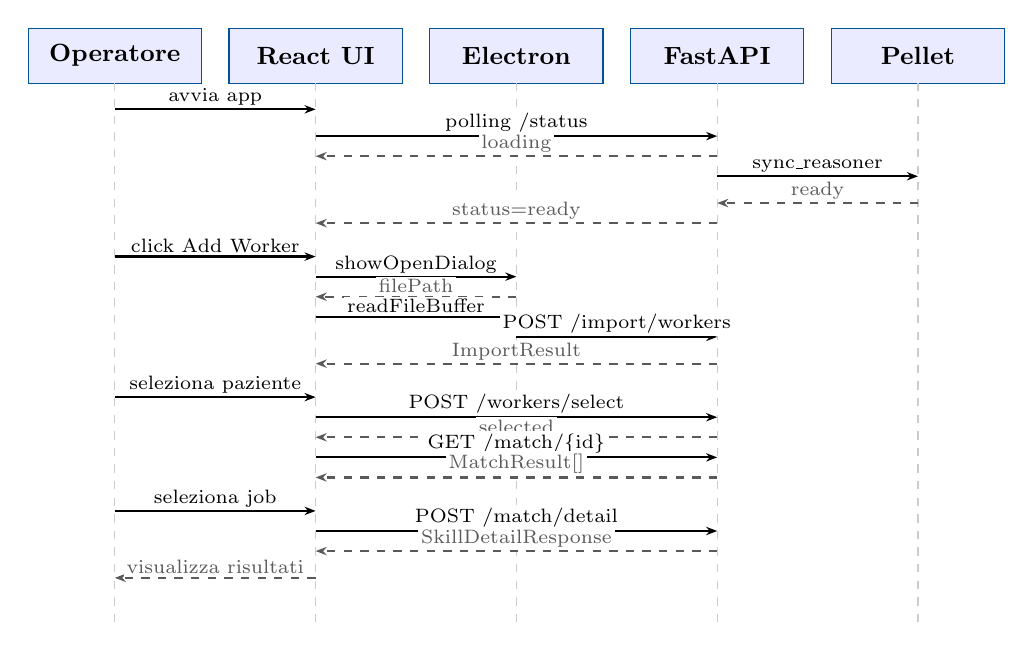
\begin{tikzpicture}[scale=0.85,
  actor/.style={rectangle, draw=rientraBlue, fill=blue!8,
                minimum width=2.2cm, minimum height=0.7cm,
                align=center, font=\small\bfseries},
  lbl/.style={font=\scriptsize, fill=white, inner sep=1pt},
  msg/.style={font=\scriptsize, above, sloped},
  arr/.style={-{Stealth[length=4pt]}, thick},
  ret/.style={-{Stealth[length=4pt]}, thick, dashed, rientraGray},
  node distance=0cm,
]
  % Lifeline headers
  \node[actor] (user)     at (0,0)   {Operatore};
  \node[actor] (react)    at (3,0)   {React UI};
  \node[actor] (electron) at (6,0)   {Electron};
  \node[actor] (api)      at (9,0)   {FastAPI};
  \node[actor] (pellet)   at (12,0)  {Pellet};

  % Lifelines
  \foreach \x in {0,3,6,9,12} {
    \draw[gray!40, dashed] (\x,-0.4) -- (\x,-8.5);
  }

  % Messages
  \draw[arr] (0,-0.8) -- node[msg, fill=white, inner sep=1pt]{avvia app} (3,-0.8);
  \draw[arr] (3,-1.2) -- node[msg, fill=white, inner sep=1pt]{polling /status} (9,-1.2);
  \draw[ret] (9,-1.5) -- node[msg, fill=white, inner sep=1pt]{loading} (3,-1.5);
  \draw[arr] (9,-1.8) -- node[msg, fill=white, inner sep=1pt]{sync\_reasoner} (12,-1.8);
  \draw[ret] (12,-2.2) -- node[msg, fill=white, inner sep=1pt]{ready} (9,-2.2);
  \draw[ret] (9,-2.5) -- node[msg, fill=white, inner sep=1pt]{status=ready} (3,-2.5);

  \draw[arr] (0,-3.0) -- node[msg, fill=white, inner sep=1pt]{click Add Worker} (3,-3.0);
  \draw[arr] (3,-3.3) -- node[msg, fill=white, inner sep=1pt]{showOpenDialog} (6,-3.3);
  \draw[ret] (6,-3.6) -- node[msg, fill=white, inner sep=1pt]{filePath} (3,-3.6);
  \draw[arr] (3,-3.9) -- node[msg, fill=white, inner sep=1pt]{readFileBuffer} (6,-3.9);
  \draw[arr] (6,-4.2) -- node[msg, fill=white, inner sep=1pt]{POST /import/workers} (9,-4.2);
  \draw[ret] (9,-4.6) -- node[msg, fill=white, inner sep=1pt]{ImportResult} (3,-4.6);

  \draw[arr] (0,-5.1) -- node[msg, fill=white, inner sep=1pt]{seleziona paziente} (3,-5.1);
  \draw[arr] (3,-5.4) -- node[msg, fill=white, inner sep=1pt]{POST /workers/select} (9,-5.4);
  \draw[ret] (9,-5.7) -- node[msg, fill=white, inner sep=1pt]{selected} (3,-5.7);
  \draw[arr] (3,-6.0) -- node[msg, fill=white, inner sep=1pt]{GET /match/\{id\}} (9,-6.0);
  \draw[ret] (9,-6.3) -- node[msg, fill=white, inner sep=1pt]{MatchResult[]} (3,-6.3);

  \draw[arr] (0,-6.8) -- node[msg, fill=white, inner sep=1pt]{seleziona job} (3,-6.8);
  \draw[arr] (3,-7.1) -- node[msg, fill=white, inner sep=1pt]{POST /match/detail} (9,-7.1);
  \draw[ret] (9,-7.4) -- node[msg, fill=white, inner sep=1pt]{SkillDetailResponse} (3,-7.4);
  \draw[ret] (3,-7.8) -- node[msg, fill=white, inner sep=1pt]{visualizza risultati} (0,-7.8);

\end{tikzpicture}%
}% end resizebox
\caption{Diagramma di sequenza semplificato per lo scenario di valutazione.}
\end{figure}

% ============================================================
\section{Known issues e debiti tecnici}
% ============================================================

\subsection{Known issues}

\begin{table}[H]
\centering
\small
\caption{Problemi noti e workaround.}
\begin{tabular}{L{3.5cm} L{5.8cm} L{3.2cm}}
\toprule
\textbf{Problema} & \textbf{Descrizione} & \textbf{Workaround} \\
\midrule
Parallelizzazione Morph-KGC su macOS &
  Morph-KGC stampa un warning e disabilita la parallelizzazione quando
  invocato come libreria su darwin. &
  Atteso e ignorabile; non impatta la correttezza. \\[4pt]
Re-reasoning dopo import lento &
  \texttt{POST /import/workers} non riesegue Pellet automaticamente;
  il matching dei nuovi pazienti richiede che l'operatore assegni
  i job e poi aggiorni. &
  Assegnare i job via ``Edit Jobs'' triggera il re-reasoning. \\[4pt]
Datatype hash in mapping.ttl &
  Le TriplesMap B/D/S mostrano un datatype con hash SHA invece di
  \texttt{xsd:integer} per i qualifier. &
  Funzionale; rigenerare il mapping dopo fix in \texttt{\_generate\_mapping()}. \\[4pt]
Duplicazione \texttt{parseConditionDescription} &
  La funzione \`{e} definita identicamente in \texttt{WorkersPage}
  e \texttt{HealthConditionWizard}. &
  Estrarre in \texttt{src/utils/icfParser.ts}. \\[4pt]
Click-outside duplicato &
  Il pattern \texttt{useClickOutside} \`{e} ripetuto in tre componenti. &
  Estrarre in \texttt{src/hooks/useClickOutside.ts}. \\[4pt]
CSS custom properties parziali &
  \texttt{HealthConditionWizard.css} usa \texttt{var()} mentre gli altri
  CSS usano valori hardcoded: sistema di theming incompleto. &
  Uniformare dichiarando variabili in \texttt{:root} di \texttt{index.css}. \\[4pt]
\texttt{python-service} non bundled &
  La distribuzione Electron non include il microservizio Python;
  richiede installazione manuale. &
  Usare \texttt{extraResources} di electron-builder con Python bundled. \\[4pt]
Porta 8000 hardcoded &
  \texttt{BASE\_URL} in \texttt{semanticService.ts} e \texttt{PYTHON\_PORT}
  in \texttt{main.js} non sono sincronizzati automaticamente. &
  Usare IPC \texttt{get-python-port} per leggere la porta dinamicamente. \\
\bottomrule
\end{tabular}
\end{table}

\subsection{Debiti tecnici}

\begin{table}[H]
\centering
\caption{Debiti tecnici identificati con priorit\`{a} e impatto.}
\begin{tabular}{L{4.5cm} L{2cm} L{6cm}}
\toprule
\textbf{Debito tecnico} & \textbf{Priorit\`{a}} & \textbf{Impatto se risolto} \\
\midrule
Estrarre \texttt{useClickOutside} & Media &
  Riduce codice duplicato in 3 componenti; testabilit\`{a} migliorata. \\[3pt]
Estrarre \texttt{useResizeObserver} & Media &
  Rimuove logica \texttt{ResizeObserver} da \texttt{JobAnalysisView}. \\[3pt]
Estrarre \texttt{icfParser.ts} & Alta &
  Elimina duplicazione critica tra WorkersPage e HealthConditionWizard. \\[3pt]
Uniformare CSS custom properties & Bassa &
  Abilita theming coerente e future variazioni di colore. \\[3pt]
Aggiungere \texttt{tsconfig.app.json} / \texttt{tsconfig.node.json} & Media &
  Documentati ma non analizzati; completare la copertura TS. \\[3pt]
Sincronizzare porta via IPC & Media &
  Elimina il rischio di disallineamento \texttt{PYTHON\_PORT}. \\[3pt]
Fix datatype hash in \texttt{mapping.ttl} & Bassa &
  Migliora leggibilit\`{a} del mapping; nessun impatto funzionale. \\[3pt]
Bundling Python in Electron & Alta &
  Abilita distribuzione self-contained senza installazione manuale. \\
\bottomrule
\end{tabular}
\end{table}

% ============================================================
\section{Validazione e testing}
% ============================================================

\subsection{Validazione dell'ontologia}

L'ontologia \texttt{Rientra.rdf} \`{e} stata validata con i seguenti
strumenti, come indicato nella documentazione dell'importer (v0.1-test):

\begin{table}[H]
\centering
\caption{Strumenti di validazione dell'ontologia e risultati.}
\begin{tabular}{L{4cm} L{3cm} L{5.5cm}}
\toprule
\textbf{Strumento} & \textbf{Versione} & \textbf{Risultato} \\
\midrule
Prot\'{e}g\'{e} & 5.6.9 &
  Caricamento e visualizzazione corretti; individui importati
  visibili nel class browser. \\[3pt]
Pellet & 2.2.0 &
  Reasoning completato senza \texttt{InconsistentOntologyException};
  propriet\`{a} SWRL materializzate. \\[3pt]
HermiT & 1.4.3.456 &
  Classificazione corretta; nessuna classe insoddisfacibile. \\[3pt]
owlready2 & $\geq$ 0.46 &
  Caricamento tramite \texttt{get\_ontology().load()}; 1.458 individui. \\
\bottomrule
\end{tabular}
\end{table}

\subsection{Test rapido del microservizio}

Dopo l'avvio e il completamento del warm-up (\texttt{status = "ready"}),
il microservizio pu\`{o} essere verificato con i seguenti comandi
\texttt{curl}:

\begin{lstlisting}[language=bash, caption={Test rapido degli endpoint principali.}]
# 1. Verifica readiness
curl http://127.0.0.1:8000/status

# 2. Lista workers
curl http://127.0.0.1:8000/workers

# 3. Lista job
curl http://127.0.0.1:8000/jobs

# 4. Condizioni ICF di un worker
curl http://127.0.0.1:8000/health-conditions/Patient1

# 5. Seleziona worker
curl -X POST http://127.0.0.1:8000/workers/select \
     -H "Content-Type: application/json" \
     -d '{"worker_id": "Patient1"}'

# 6. Match results
curl http://127.0.0.1:8000/match/Patient1

# 7. Dettaglio skill per coppia (worker, job)
curl -X POST http://127.0.0.1:8000/match/detail \
     -H "Content-Type: application/json" \
     -d '{"worker_id":"Patient1","job_id":"Job_AssemblyWorker"}'

# 8. Documentazione interattiva
open http://127.0.0.1:8000/docs
\end{lstlisting}

\noindent La documentazione interattiva Swagger UI (\texttt{/docs}) permette di
eseguire ogni endpoint direttamente dal browser, con auto-compilazione
dei campi e visualizzazione dello schema JSON. \`{E} lo strumento
raccomandato per la verifica manuale durante lo sviluppo.

% ============================================================
\section{Note su provenienza dati, licenze e privacy}
% ============================================================

\subsection{Provenienza dati O*NET}

I punteggi di importanza delle Skill e Abilities usati nell'ontologia
Rientr@ sono derivati dal database \textbf{O*NET} (\textit{Occupational
Information Network}), mantenuto dal U.S. Department of Labor/Employment
and Training Administration (USDOL/ETA).

\begin{table}[H]
\centering
\caption{Dati O*NET nell'ontologia Rientr@.}
\begin{tabular}{L{4cm} L{8.5cm}}
\toprule
\textbf{Aspetto} & \textbf{Dettaglio} \\
\midrule
Fonte & O*NET OnLine (\texttt{onetonline.org}), USDOL/ETA \\
Licenza & Pubblico dominio (Creative Commons CC-BY 4.0 per i dati aggregati) \\
Utilizzo nell'ontologia & Punteggi \texttt{hasScore} [0--100] per ogni \texttt{Job\_Descriptor} \\
Versione & Incorporata staticamente in \texttt{Rientra.rdf}; aggiornamenti richiedono rigenerazione dell'ontologia \\
Classificazione SOC & Standard Occupational Classification del Bureau of Labor Statistics \\
\bottomrule
\end{tabular}
\end{table}

\subsection{Dati ICF e OMS}

La classificazione ICF \`{e} pubblicata dall'\textbf{Organizzazione
Mondiale della Sanit\`{a}} (OMS/WHO, 2001). I codici e le descrizioni
testuali incluse nell'ontologia sono estratti dalla versione ufficiale
ICF e dai core set clinici sviluppati in collaborazione con il
\textit{ICF Research Branch}. L'uso \`{e} consentito per scopi di
ricerca e applicazioni non commerciali in ambito sanitario.

\subsection{Dati clinici e privacy}

\begin{warningbox}[Dati sensibili --- Note di conformit\`{a}]
I dati importati tramite \texttt{POST /import/workers} includono
informazioni cliniche personali (codici ICF con qualifier, dati
anagrafici). Il sistema nella versione attuale (v0.1-test) \textbf{non
implementa}:
\begin{itemize}[noitemsep]
  \item Autenticazione o autorizzazione degli utenti.
  \item Cifratura dei dati in transito (HTTP, non HTTPS).
  \item Controllo di accesso ai file RDF su disco.
  \item Anonimizzazione o pseudonimizzazione automatica.
\end{itemize}
Per un deploy in ambiente clinico \`{e} obbligatorio valutare la
conformit\`{a} al GDPR (Regolamento UE 2016/679) e alle normative
nazionali sulla protezione dei dati sanitari, introducendo almeno:
autenticazione locale, cifratura TLS, e gestione dei log di accesso.
\end{warningbox}

% ============================================================
\section{Configurazione IDE e ambiente di sviluppo consigliato}
% ============================================================

\subsection{Strumenti consigliati}

\begin{table}[H]
\centering
\caption{Strumenti consigliati per lo sviluppo del progetto Rientr@.}
\begin{tabular}{L{4cm} L{3cm} L{5.5cm}}
\toprule
\textbf{Strumento} & \textbf{Versione} & \textbf{Utilizzo} \\
\midrule
Visual Studio Code & $\geq$ 1.85 &
  IDE principale per TypeScript/React e Python. \\[3pt]
Prot\'{e}g\'{e} & 5.6.x &
  Editor ontologie OWL; validazione e browsing del grafo RDF. \\[3pt]
Insomnia / Postman & qualsiasi &
  Test manuale degli endpoint REST; importazione da \texttt{/openapi.json}. \\[3pt]
Java 11+ (Temurin) &  $\geq$ 11 &
  Runtime richiesto da Pellet; Eclipse Temurin \`{e} la distribuzione
  raccomandata (gratuita, LTS). \\[3pt]
Node.js & $\geq$ 20 LTS &
  Runtime per Electron e Vite. \\[3pt]
Python & 3.11--3.12 &
  Runtime del microservizio; evitare 3.13+ finch\'{e} owlready2 non
  aggiorna il supporto. \\
\bottomrule
\end{tabular}
\end{table}

\subsection{Estensioni VSCode raccomandate}

\begin{table}[H]
\centering
\caption{Estensioni VSCode per il progetto Rientr@.}
\small
\begin{tabular}{L{5.5cm} L{7cm}}
\toprule
\textbf{Estensione} & \textbf{Motivazione} \\
\midrule
\texttt{ms-python.python} &
  IntelliSense, debugging e linting Python. \\[3pt]
\texttt{ms-python.pylance} &
  Type checking Python avanzato; rileva errori di tipo in owlready2. \\[3pt]
\texttt{dbaeumer.vscode-eslint} &
  Integrazione ESLint con flat config; mostra warning inline. \\[3pt]
\texttt{bradlc.vscode-tailwindcss} &
  Autocompletamento classi Tailwind nelle stringhe TypeScript. \\[3pt]
\texttt{esbenp.prettier-vscode} &
  Formattazione automatica TypeScript/JSON/CSS. \\[3pt]
\texttt{ms-vscode.vscode-typescript-next} &
  Supporto TypeScript sperimentale; utile con TS 5.9+. \\[3pt]
\texttt{GraphQL.vscode-graphql-syntax} &
  Syntax highlighting per file Turtle (\texttt{.ttl}) del mapping R2RML. \\[3pt]
\texttt{redhat.vscode-yaml} &
  Validazione YAML per eventuali file di configurazione. \\
\bottomrule
\end{tabular}
\end{table}

\subsection{Configurazione \texttt{.vscode/settings.json} consigliata}

\begin{lstlisting}[language=Java, caption={Impostazioni VSCode raccomandate per Rientr@.}]
{
  "python.defaultInterpreterPath": "./python-service/.venv/bin/python3",
  "python.analysis.typeCheckingMode": "off",  // owlready2 no stubs
  "editor.formatOnSave": true,
  "editor.defaultFormatter": "esbenp.prettier-vscode",
  "[python]": {
    "editor.defaultFormatter": "ms-python.black-formatter"
  },
  "eslint.useFlatConfig": true,
  "files.associations": { "*.ttl": "turtle" },
  "editor.rulers": [88]  // PEP 8 line length
}
\end{lstlisting}

% ============================================================
\section{Changelog versioni del documento}
% ============================================================

{\footnotesize
\begin{longtable}{L{1.4cm} L{2.8cm} L{8.3cm}}
\toprule
\textbf{Vers.} & \textbf{Data} & \textbf{Modifiche principali} \\
\midrule
\endhead
1.0 & Maggio 2026 &
  Prima versione. Documentazione di \texttt{main.py}: entry point
  FastAPI, lifespan, CORS, guard, tutti i 17 endpoint. \\[3pt]
1.1 & Maggio 2026 &
  Aggiunto \texttt{models.py}: 19 modelli Pydantic v2 con motivazioni,
  convenzioni, diagramma relazioni. \\[3pt]
1.2 & Maggio 2026 &
  Aggiunto \texttt{reasoner.py}: caricamento ontologia, Pellet,
  snapshot cache, tutte le query SPARQL (Q0--Q4), mutazioni, lock. \\[3pt]
1.3 & Maggio 2026 &
  Aggiunta ontologia Rientr@ v3.1: struttura, classi, propriet\`{a},
  core set ICF, 13 regole SWRL. Setup e configurazione. \\[3pt]
1.4 & Maggio 2026 &
  Aggiunto \texttt{importer.py}: pipeline RDB2RDF, Morph-KGC,
  VIEW SQL, iniezione testuale, problema boolean Pellet. \\[3pt]
1.5 & Maggio 2026 &
  Aggiunto layer Electron: \texttt{main.js} e \texttt{preload.js}
  con architettura a tre processi. \\[3pt]
1.6 & Maggio 2026 &
  Aggiunto layer React: \texttt{App.tsx}, \texttt{main.tsx},
  \texttt{index.css}, struttura \texttt{src/}. \\[3pt]
1.7 & Maggio 2026 &
  Aggiunta documentazione componenti React: \texttt{HomePage},
  \texttt{WorkersPage}, \texttt{JobAnalysisView},
  \texttt{HealthConditionWizard}. Prima versione. \\[3pt]
1.8 & Maggio 2026 &
  Riscrittura approfondita dei componenti React con stessa profondit\`{a}
  delle sezioni Python. \\[3pt]
1.9 & Maggio 2026 &
  Aggiunta motivazione WHY su 23 sezioni precedentemente prive. \\[3pt]
2.0 & Maggio 2026 &
  Aggiunta documentazione CSS approfondita (WorkersPage, JobAnalysis,
  HealthConditionWizard): token, pattern, animazioni. \\[3pt]
2.1 & Maggio 2026 &
  Aggiunto \texttt{semanticService.ts}, \texttt{package.json},
  \texttt{vite.config.ts}, \texttt{tsconfig.json}, \texttt{eslint.config.js},
  \texttt{start.sh}, script di utilit\`{a}. \\[3pt]
2.2 & Maggio 2026 &
  Aggiunti indici figure/tabelle/listing, glossario 40 termini
  (5 categorie), 8 WHY aggiuntivi. \\[3pt]
2.3 & Maggio 2026 &
  Correzioni tipografiche: TOC overflow, widow sections, 40+ overfull
  hbox risolti, copertina ridisegnata. \\[3pt]
2.4 & Maggio 2026 &
  Aggiunto: scenari d'uso, diagramma sequenza UML, known issues,
  debiti tecnici, validazione ontologia, test curl, O*NET/ICF licenze,
  note GDPR, configurazione IDE e VSCode. \\
\bottomrule
\end{longtable}
}% end footnotesize


\end{document}
